\documentclass{OFbook}
\setcounter{secnumdepth}{4}
% \nofiles

\usepackage[dvipdfmx]{color}
\usepackage[dvipdfmx]{graphicx}
\usepackage{mediabb}
\graphicspath{{./fig/pdf/}}
\usepackage{ltxtable}

\usepackage[deluxe]{otf}
\usepackage{lmodern}
\usepackage[T1]{fontenc}
\usepackage{textcomp}
\usepackage[utf8]{inputenc}
\usepackage{amsmath,amssymb}
\usepackage{bm}

\usepackage[dvipdfm,
 bookmarks=true,
 bookmarksnumbered=true,
 pdftitle={OpenFOAM User Guide},
 pdfsubject={Japanese edition},
 pdfauthor={The Open CAE Society of Japan (www.opencae.jp)},
 pdfkeywords={OpenFOAM},
 colorlinks=true,
 linkcolor=red,
 filecolor=blue,
 urlcolor=blue
 ]{hyperref}[2007/12/08]
\usepackage{atbegshi}
\AtBeginShipoutFirst{\special{pdf:tounicode EUC-UCS2}}

\usepackage{OFmacros}

\usepackage{makeidx}
\makeindex
\def\seename{$\Longrightarrow$}

\title{ユーザガイド和訳}
\author{一般社団法人 オープンCAE学会}
\version{2.3.0}
\def\thepage{U-\arabic{page}}

\begin{document}

\maketitle
\frontmatter

\begin{OFdeclaration}
%#! platex UserGuideJa

Copyright \copyright{} 2006--2012 一般社団法人 オープンCAE学会

\vskip\Cvs

このユーザガイド和訳は,
一般社団法人 オープンCAE学会の責任のもとで公開しております.
本書に関するご意見等がございましたら,
当学会事務局 (\href{mailto:office@opencae.jp}{office@opencae.jp}) までご連絡ください.

\vskip2\Cvs

下記に示した原文の著作権表示に従い,
GNU Free Documentation Licenseのバージョン1.2に基づいて,
本和訳文書の複製・配布・改変が許可されています.

\vskip.5\Cvs

次ページ以降にGNU Free Documentation Licenseを掲載します.

\vskip.5\Cvs

\hfill 一般社団法人 オープンCAE学会\par

\vskip.5\Cvs

\noindent
Typeset in p\LaTeX.


\vskip3\Cvs

\section*{\gtfamily\mdseries 原文著作権表示}
Copyright \copyright{} 2011 OpenFOAM Foundation.

\vskip\Cvs

Permission is granted to copy, distribute and/or modify this document under the terms
of the GNU Free Documentation License, Version 1.2 published by the Free Software
Foundation; with no Invariant Sections, no Back-Cover Texts and one Front-Cover Text:
``Available free from openfoam.org.'' A copy of the license is included in the section
entitled ``GNU Free Documentation License''.

\vskip\Cvs

This document is distributed in the hope that it will be useful, but WITHOUT ANY
WARRANTY; without even the implied warranty of MERCHANTABILITY or FITNESS
FOR A PARTICULAR PURPOSE.

%#! platex UserGuideJa

\section*{Trademarks}
\OFemph{ANSYS} is a registered trademark of ANSYS Inc.\par
\OFemph{CFX} is a registered trademark of AEA Technology Engineering Software Ltd.\par
\OFemph{CHEMKIN} is a registered trademark of Sandia National Laboratories\par
\OFemph{CORBA} is a registered trademark of Object Management Group Inc.\par
\OFemph{openDX} is a registered trademark of International Business Machines Corporation\par
\OFemph{EnSight} is a registered trademark of Computational Engineering International Ltd.\par
\OFemph{AVS}/Express is a registered trademark of Advanced Visual Systems Inc.\par
\OFemph{Fluent} is a registered trademark of Fluent Inc.\par
\OFemph{GAMBIT} is a registered trademark of Fluent Inc.\par
\OFemph{Fieldview} is a registered trademark of Intelligent Light\par
\OFemph{Icem-CFD} is a registered trademark of ICEM Technologies GmbH\par
\OFemph{I-DEAS} is a registered trademark of Structural Dynamics Research Corporation\par
\OFemph{JAVA} is a registered trademark of Sun Microsystems Inc.\par
\OFemph{Linux} is a registered trademark of Linus Torvalds\par
\OFemph{MICO} is a registered trademark of MICO Inc.\par
\OFemph{ParaView} is a registered trademark of Kitware\par
\OFemph{STAR-CD} is a registered trademark of Computational Dynamics Ltd.\par
\OFemph{UNIX} is a registered trademark of The Open Group\par
\vskip.5\Cvs
OpenFOAM\textregistered{} is a registered trademark of OpenCFD Ltd.\par

\end{OFdeclaration}

\tableofcontents

\mainmatter
../../../ProgrammersGuideJa/chapter1.tex
%#! platex UserGuideJa
\chapter{チュートリアル}
\label{chap:2}
この章ではOpenFOAMを動かす基本的な手順をユーザに説明することを主な目標として,
OpenFOAMのいくつかのテストケースで,設定,
シミュレーション,および後処理のプロセスを詳しく記述します.
\OFpath{\$FOAM\_TUTORIALS}のディレクトリには
OpenFOAMが提供するすべてのソルバと
多くのユーティリティを使い方を示す数多くのケースがあります.
チュートリアルを始める前にユーザは最初にOpenFOAMが正しく
インストールされていることを確かめなければなりません.

チュートリアルのケースは\OFtool{blockMesh}の前処理ツールを使用して記述し,
OpenFOAMのソルバで動かし,\OFtool{paraFoam}を使用して後処理を行います.
OpenFOAMのサポートするサードパーティの後処理ツールにアクセスする
ユーザには次の選択肢があります.
\OFtool{paraFoam}を使用しチュートリアルを進めるか,
または後処理が必要な際に
\autoref{chap:6}で述べるサードパーティ製品の使い方を参照するかです.

すべてのチュートリアルのコピーは
OpenFOAMをインストールしたチュートリアルのディレクトリから利用できます.
チュートリアルは,流れのタイプによるディレクトリと
ソルバのサブディレクトリにまとめられています.
例えば
\index{icoFoam@\OFtool{icoFoam}!ソルバ}%
\index{ソルバ!icoFoam@\OFtool{icoFoam}}%
\OFtool{icoFoam}のケースはすべて
\OFpath{incompressible/icoFoam}サブディレクトリの中に置かれています.
ここでincompressibleが流れのタイプを表しています.
ユーザがさまざまな例題を実施するときには,
\index{tutorials@\OFpath{tutorials}!ディレクトリ}%
\index{ディレクトリ!tutorials@\OFpath{tutorials}}%
\OFpath{tutorials}ディレクトリをローカルの実行ディレクトリに
コピーすることをお勧めします.
そのためには,次のようにタイプすることで容易にコピーすることができます.
\begin{OFverbatim}[terminal]
mkdir -p $FOAM_RUN
cp -r $FOAM_TUTORIALS $FOAM_RUN
\end{OFverbatim}%$



\section{天井駆動のキャビティ流れ}
\label{sec:2.1}
\index{てんじょうくどうのキャビティながれ@天井駆動のキャビティ流れ}%
\index{チュートリアル!てんじょうくどうのキャビティながれ@天井駆動のキャビティ流れ}%
\index{キャビティながれ@キャビティ流れ}%
このチュートリアルは2次元正方形領域の等温非圧縮性流れに関して,
前処理,計算,後処理する方法を解説します.
\autoref{fig:2.1}に
正方形のすべての境界が壁面境界とした形状を示します.
上の壁面境界は$x$軸方向に$1\unit{m/s}$の速度ではたらき,
他の三つの壁面境界は静止しています.
チュートリアルにおいてはこれを解くにあたって,まず
\index{ながれ@流れ!そうりゅう@層流}%
層流を仮定し,
層流等温非圧縮性流れのための\OFtool{icoFoam}ソルバを使用し
均一メッシュ上で解きます.
チュートリアルでは,
メッシュの解像度の増加や壁方向への勾配の影響を調べます.
これにより流れの
\index{Reynoldsすう@Reynolds数}%
Reynolds数を増加させ,
\index{pisoFoam@\OFtool{pisoFoam}!ソルバ}%
\index{ソルバ!pisoFoam@\OFtool{pisoFoam}}%
\OFtool{pisoFoam}ソルバを
\index{ながれ@流れ!らんりゅう@乱流}%
乱流,等温,非圧縮性流れに使用します.


\begin{figure}[ht]
 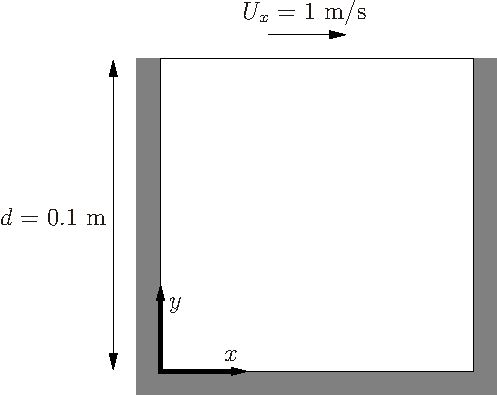
\includegraphics{fig-2-1}
 \caption{天井駆動キャビティのジオメトリ}
 \label{fig:2.1}
\end{figure}


\subsection{前処理}
\label{ssec:2.1.1}
ケースはOpenFOAMでケースファイルを編集することで設定します.
ケースファイルは\OFthirdparty{emacs}や\OFthirdparty{vi},
\OFthirdparty{gedit},\OFthirdparty{kate},\OFthirdparty{nedit}などの
テキストエディタで作成・編集します.
OpenFOAMでは,初心者でも理解できるような
わかりやすいキーワードをもつディクショナリ形式を用いて入出力を行うため,
ファイルを直接編集することが可能です.

解析ケースはメッシュ,物理量,物性,制御パラメータなどの要素を
含んでいますが\autoref{sec:4.1}において示すように,
多くのCFDソフトが一つのファイルにこれらのデータを格納するのに対し,
OpenFOAMは一連のファイルセットとして解析ケースディレクトリに格納します.
解析ケースのディレクトリには,
(最初のチュートリアルの例題が単純にcavityであるように)
わかりやすい名前を与えます.
解析ケースを編集・実行する前の準備として,
まず解析対象のディレクトリに移動します.
\begin{OFverbatim}[terminal]
cd $FOAM_RUN/tutorials/incompressible/icoFoam/cavity
\end{OFverbatim}%$

\subsubsection{メッシュ生成}
\label{sssec:2.1.1.1}
\index{ざひょうじく@座標軸!みぎてけいちょっこうCartesian@右手系直交Cartesian}%
OpenFOAMは常に3次元Cartesian
\index{ざひょうけい@座標系}%
座標系で動くため,
全てのジオメトリを3次元で生成します.
OpenFOAMはデフォルトの設定において問題を3次元として解きますが,
2次元を解く場合は,解決が必要でない(第3)次元方向に垂直な境界に
\textgt{特別な}
\index{empty@\OFboundary{empty}!きょうかいじょうけん@境界条件}%
\index{きょうかいじょうけん@境界条件!empty@\OFboundary{empty}}%
\OFboundary{empty}という境界条件を指定します.

$x$--$y$平面上の一辺の長さの正方形からなるキャビティの領域に,
まず$20 \times 20$セルの均一なメッシュを設定します.
このブロック構造を\autoref{fig:2.2}に示します.


\begin{figure}[ht]
 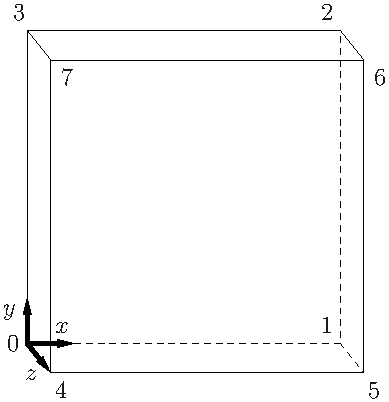
\includegraphics{fig-2-2}
 \caption{キャビティのメッシュのブロック構造}
 \label{fig:2.2}
\end{figure}


OpenFOAMで提供されるメッシュ・ジェネレータ\OFtool{blockMesh}は
\OFpath{constant/polyMesh}ディレクトリにある入力ディクショナリ
\index{blockMeshDict@\OFdictionary{blockMeshDict}!ディクショナリ}%
\index{ディクショナリ!blockMeshDict@\OFdictionary{blockMeshDict}}%
\OFdictionary{blockMeshDict}で指定された
記述からメッシュを生成します.
このケースの\OFdictionary{blockMeshDict}は,以下のとおりです.
\begin{OFverbatim}[file, linenum]
/*--------------------------------*- C++ -*----------------------------------*\
| =========                 |                                                 |
| \\      /  F ield         | OpenFOAM: The Open Source CFD Toolbox           |
|  \\    /   O peration     | Version:  2.3.0                                 |
|   \\  /    A nd           | Web:      www.OpenFOAM.org                      |
|    \\/     M anipulation  |                                                 |
\*---------------------------------------------------------------------------*/
FoamFile
{
    version     2.0;
    format      ascii;
    class       dictionary;
    object      blockMeshDict;
}
// * * * * * * * * * * * * * * * * * * * * * * * * * * * * * * * * * * * * * //

convertToMeters 0.1;

vertices        
(
    (0 0 0)
    (1 0 0)
    (1 1 0)
    (0 1 0)
    (0 0 0.1)
    (1 0 0.1)
    (1 1 0.1)
    (0 1 0.1)
);

blocks          
(
    hex (0 1 2 3 4 5 6 7) (20 20 1) simpleGrading (1 1 1)
);

edges           
(
);

boundary
(
    movingWall 
    {
        type wall;
        faces
        (
            (3 7 6 2)
        );
    }
    fixedWalls 
    {
        type wall;
        faces
        (
            (0 4 7 3)
            (2 6 5 1)
            (1 5 4 0)
        );
    }
    frontAndBack 
    {
        type empty;
        faces
        (
            (0 3 2 1)
            (4 5 6 7)
        );
    }
);

mergePatchPairs 
(
);

// ************************************************************************* //
\end{OFverbatim}
ファイルの最初(1--7行目)にはバナー形式のヘッダ情報があり,
それから波括弧 (\verb|{|\ldots\verb|}|) で囲まれる
\OFsubdictionary{FoamFile}サブディクショナリの中に,
ファイルの情報が記述されています.

簡便化とスペースの都合上,今後ケースファイルを引用する際は,
バナーと\OFsubdictionary{FoamFile}サブディクショナリを含む
ファイルヘッダは省きます.

ファイルの最初には,ブロックの頂点の座標
\index{vertices@\OFkeyword{vertices}!キーワード}%
\index{キーワード!vertices@\OFkeyword{vertices}}%
\OFkeyword{vertices}を指定します.
それから,頂点名とセル番号から
\index{blocks@\OFkeyword{blocks}!キーワード}%
\index{キーワード!blocks@\OFkeyword{blocks}}%
\OFkeyword{blocks}(ここでは一つのみ)を定義します.
そして最後に境界パッチを定義します.
\OFdictionary{blockMeshDict}ファイルの記述の詳細を理解するには
\autoref{sec:5.3}を参照してください.

メッシュは\OFdictionary{blockMeshDict}ファイル上で
\OFtool{blockMesh}を実行すると生成されます.
ケースディレクトリ内から以下をターミナルに入力するだけで実行されます.
\begin{OFverbatim}[terminal]
blockMesh
\end{OFverbatim}
\OFtool{blockMesh}の実行状況はターミナルウィンドウに表示されます.
\index{blockMeshDict@\OFdictionary{blockMeshDict}!ディクショナリ}%
\index{ディクショナリ!blockMeshDict@\OFdictionary{blockMeshDict}}%
\OFdictionary{blockMeshDict}ファイルに誤りがあった場合,
エラーメッセージが表示され,
ファイルのどの行に問題があるかを教えてくれます.
今この段階でエラーメッセージが出ることはないでしょう.

\subsubsection{境界条件と初期条件}
\label{sssec:2.1.1.2}
メッシュの生成が完了すると,物理的条件の初期状態を確認することができます.
このケースは開始時刻がに設定されているので解析領域の初期状態のデータは
\OFpath{cavity}ディレクトリの\OFpath{0}という
サブディレクトリに格納されています.
\OFpath{0}には\OFpath{p}と\OFpath{U}の二つのファイルがあり,
圧力 ($p$) と速度 ($U$) の初期値と境界条件を設定する必要があります.
\OFpath{p}のファイルを例に説明します.
\begin{OFverbatim}[file, linenum=17]
dimensions      [0 2 -2 0 0 0 0];

internalField   uniform 0;

boundaryField
{
    movingWall
    {
        type            zeroGradient;
    }

    fixedWalls
    {
        type            zeroGradient;
    }

    frontAndBack
    {
        type            empty;
    }
}

// ************************************************************************* //
\end{OFverbatim}
物理的条件のデータファイルには三つの主要な項目があります.
\begin{description}
 \item[dimensions]
\index{dimensions@\OFkeyword{dimensions}!キーワード}%
\index{キーワード!dimensions@\OFkeyword{dimensions}}%
            物理量の次元を指定します.ここでは動圧,つまり
            $\unit*{m^{2}s^{-2}}$(\autoref{ssec:4.2.6}に詳述)とします.
 \item[internalField]
\index{internalField@\OFkeyword{internalField}!キーワード}%
\index{キーワード!internalField@\OFkeyword{internalField}}%
            内部の物理量は単一の値で記述すれば一様となり,
            一様でない場合はすべての値を指定する必要があります
            (\autoref{ssec:4.2.8}に詳述).
 \item[boundaryField]
\index{boundaryField@\OFkeyword{boundaryField}!キーワード}%
\index{キーワード!boundaryField@\OFkeyword{boundaryField}}%
            境界面の物理量は境界条件と境界パッチに与えるデータを
            記述します(\autoref{ssec:4.2.8}に詳述).
\end{description}
このキャビティ流れの解析ケースでは境界は壁面のみですが,
二つのパッチに分けて以下のように名付けます.
(1) キャビティの固定された側面と底面用の\OFpatch{fixedwall}と,
(2) キャビティの駆動天井面用の\OFpatch{movingwall}です.
どちらも$p$が\OFkeyword{zeroGradient}ですが,
これは圧力の境界に垂直な方向の勾配が$0$であるということです.
\OFpatch{frontAndBack}は2次元の問題の場合の表裏の平面を示していて,
本ケースでは当然\OFkeyword{empty}となっています.

このケースでは,もっともよく目にするものでありますが,
物理量の初期条件が\OFkeyword{uniform}(一様)になっています.
ここでは圧力は動圧のみの非圧縮ケースであるため,
絶対値は解析と関係ないので便宜上\texttt{uniform 0}としています.

\OFpath{0/U}の速度のファイルにおいても同様です.
\OFkeyword{dimensions}は速度であり,
内部の初期条件はベクトル量で3成分とも$0$を意味する
\texttt{uniform (0 0 0)}になっています(\autoref{ssec:4.2.5}に詳述).

速度の境界条件は\OFpatch{frontAndBack}パッチと同じ条件です.
その他の境界は壁ですが,
\OFpatch{fixedWall}ではすべりなし (no-slip) 条件を仮定するため,
\index{value@\OFkeyword{value}!キーワード}%
\index{キーワード!value@\OFkeyword{value}}%
\OFkeyword{value}が\texttt{uniform (0 0 0)}の\OFkeyword{fixedValue}とします.
上面は$x$方向に$1\unit{m/s}$で移動するので,
こちらも\OFkeyword{fixedValue}ですが,
\OFkeyword{value}は\texttt{uniform (1 0 0)}とします.

\subsubsection{物性値}
\label{sssec:2.1.1.3}
ケースの物理量は,名前に\OFpath{...Properties}という語尾を与えられて
ディクショナリに保存され,\OFpath{Dictionaries}ディレクトリツリーに置かれます.
\index{icoFoam@\OFtool{icoFoam}!ソルバ}%
\index{ソルバ!icoFoam@\OFtool{icoFoam}}%
\OFtool{icoFoam}ケースでは,
\index{transportProperties@\OFdictionary{transportProperties}!ディクショナリ}%
\index{ディクショナリ!transportProperties@\OFdictionary{transportProperties}}%
\OFdictionary{transportProperties}ディクショナリに保存される
動粘性係数を指定するだけです.
\OFdictionary{transportProperties}ディクショナリを開いてその中身を確認したり,
編集することができますので,
\index{ねんせいけいすう@粘性係数!どう@動\jdash}%
動粘性係数が正しくセットされることを確かめてください.
動粘性係数は,\OFkeyword{nu} (数式中で$\nu$と書かれるギリシア文字の音声ラベル)
というキーワードになります.
まず最初に,このケースはReynolds数を$10$で計算します.
\index{Reynoldsすう@Reynolds数}%
Reynolds数は次のように定義されます.
\begin{align}
 \label{eq:2.1}
 \nRe = \frac{d|\bm{U}|}{\nu}
\end{align}
$d$と$\bm{U}$はそれぞれ特性長さと速度を表し,
$\nu$は動粘性係数を表します.
ここで,$d = 0.1\unit{m}$,$|\bm{U}| = 1\unit{m\,s^{-1}}$,
$\nRe = 10$とすると,$\nu = 0.01\unit{m^{2}s^{-1}}$となります.
動粘性係数の適切な設定は以下のようになります.
\begin{OFverbatim}[file, linenum=17]

nu              nu [0 2 -1 0 0 0 0] 0.01;


// ************************************************************************* //
\end{OFverbatim}

\subsubsection{制御}
\label{sssec:2.1.1.4}
計算時間の制御,解のデータの読み書きに関する入力データは,
\index{controlDict@\OFdictionary{controlDict}!ディクショナリ}%
\index{ディクショナリ!controlDict@\OFdictionary{controlDict}}%
\OFdictionary{controlDict}ディクショナリから読み取られます.
これは\OFpath{system}ディレクトリにありますので,
ケースを制御するファイルとして参照してください.

まず最初にスタート・停止時刻と時間ステップを設定しなければなりません.
OpenFOAMは,柔軟性の高い時間制御を提供しますが,
詳しくは\autoref{sec:4.3}で述べます.このチュートリアルでは,
時刻$t = 0$から実行を始めたいと思います.
つまり,OpenFOAMは\OFpath{0}というディレクトリから
場のデータを読む必要があることになります
(ケースファイル構造の詳しい情報に関しては\autoref{sec:4.1}を見てください).
したがって,
\index{startFrom@\OFkeyword{startFrom}!キーワード}%
\index{キーワード!startFrom@\OFkeyword{startFrom}}%
\OFkeyword{startFrom}キーワードを
\index{startTime@\OFkeyword{startTime}!キーワードエントリ}%
\index{キーワードエントリ!startTime@\OFkeyword{startTime}}%
\OFkeyword{startTime}に設定して,
次に
\index{startTime@\OFkeyword{startTime}!キーワード}%
\index{キーワード!startTime@\OFkeyword{startTime}}%
\OFkeyword{startTime}キーワードを0に指定します.

終了時刻には,流れがキャビティ周りを循環している定常解に達することを
目標にするわけですが,概して,流体は層流で定常状態に到達するために
領域を10回通り抜けなければなりません.
このケースでは,入口も出口もないので,流れが解析領域を通り抜けません.
代わりに,ふたがキャビティを10回移動する時刻 (すなわち$1\unit{s}$) を
終了時刻としてセットしてもいいでしょう.
実際は,後の知見により,$0.5\unit{s}$で十分であるとわかるので,
この値を採用しましょう.
この終了時刻を指定するために,\OFkeyword{stopAt}キーワードとして
\OFkeyword{endTime}を指定して,
\index{endTime@\OFkeyword{endTime}!キーワード}%
\index{キーワード!endTime@\OFkeyword{endTime}}%
\OFkeyword{endTime}キーワードを0.5に設定しなければなりません.

次に,時間ステップを設定する必要がありますが,
これはキーワード\OFkeyword{deltaT}によって表されます.
\OFtool{icoFoam}を動かすとき,時間の精度と安定性を達成するために,
$1$未満のCourant数が必要です.
\index{Courantすう@Courant数}%
Courant数は以下のように定義されます.
\begin{align}
 \label{eq:2.2}
  \nCo = \frac{\Delta t|\bm{U}|}{\Delta x}
\end{align}
$\Delta t$は時間ステップ,$|\bm{U}|$はセルを通る流速の大きさ,
そして$\Delta x$は流速方向のセルサイズです.
流速が領域内で変化しても必ず$\nCo < 1$を成り立たせる必要があります.
だから,最も悪い場合(つまり,大きな流速と小さなセルサイズの
組合わせによる最大の$\nCo$)を元に$\Delta t$を決定します.
ここでは,セルサイズは解析領域中全域で固定されているので,
最大$\nCo$はふた付近に生じ,$1\unit{m\,s^{-1}}$に近い流速になるでしょう.
\begin{align}
 \label{eq:2.3}
  \Delta x = \frac{d}{n} = \frac{0.1}{20} = 0.005\unit{m}
\end{align}
したがって,領域中で$1$以下のCourant数を達成するために,
\index{じかんステップ@時間ステップ}%
時間ステップ\OFkeyword{deltaT}を次のように設定しなくてはいけません.
\begin{align}
 \label{eq:2.4}
  \Delta t = \frac{\nCo\Delta x}{|\bm{U}|}
  = \frac{1 \times 0.005}{1} = 0.005\unit{s}
\end{align}
シミュレーションが進行するとき,
後処理パッケージで後から見ることができるように,
ある一定の時間間隔での結果の書き出しをもとめるため,
\index{writeControl@\OFkeyword{writeControl}!キーワード}%
\index{キーワード!writeControl@\OFkeyword{writeControl}}%
\OFkeyword{writeControl}キーワードは結果が書かれる時刻を決めるための
いくつかのオプションを提示します.
\index{timeStep@\OFkeyword{timeStep}!キーワードエントリ}%
\index{キーワードエントリ!timeStep@\OFkeyword{timeStep}}%
\OFkeyword{timeStep}オプションは,
結果が$n$回の時間ステップごとに結果を書き出すということを意味し,
そのときの値は
\index{writeInterval@\OFkeyword{writeInterval}!キーワード}%
\index{キーワード!writeInterval@\OFkeyword{writeInterval}}%
\OFkeyword{writeInterval}キーワードで指定されます.
$0.1, 0.2, \ldots, 0.5\unit{s}$で結果を書きたいとしましょう.
したがって,$0.005\unit{s}$の時間ステップなので,
時間ステップ$20$回ごとに結果を出力する必要があります.
よって\OFkeyword{writeInterval}に20を設定します.

OpenFOAMは\autoref{sec:4.1}で議論するデータセットを
書き込むごとに例えば$0.1\unit{s}$という現在時刻にちなんで名付けられた
新しいディレクトリを作成します.
\index{icoFoam@\OFtool{icoFoam}!ソルバ}%
\index{ソルバ!icoFoam@\OFtool{icoFoam}}%
\OFtool{icoFoam}ソルバでは,
\index{U@\OFkeyword{U}!フィールド}%
\index{フィールド!U@\OFkeyword{U}}%
\OFkeyword{U}や
\index{p@\OFkeyword{p}!フィールド}%
\index{フィールド!p@\OFkeyword{p}}%
\OFkeyword{p}の各項目ごとに結果を時刻ディレクトリに書き込みます.
このケースでは,\OFdictionary{controlDict}の記述内容は以下のとおりです.
\begin{OFverbatim}[file, linenum=17]

application     icoFoam;

startFrom       startTime;

startTime       0;

stopAt          endTime;

endTime         0.5;

deltaT          0.005;

writeControl    timeStep;

writeInterval   20;

purgeWrite      0;

writeFormat     ascii;

writePrecision  6;

writeCompression off;

timeFormat      general;

timePrecision   6;

runTimeModifiable true;


// ************************************************************************* //
\end{OFverbatim}

\subsubsection{離散化と線形ソルバの設定}
\label{sssec:2.1.1.5}
ユーザは\OFdictionary{fvSchemes}ディクショナリ (\OFpath{system}ディレクトリ) 内で
有限体積離散化法を選択するかどうか指定します.
線形方程式ソルバと許容値および他のアルゴリズムコントロールの指定は
\OFdictionary{fvSolution}ディクショナリ内に作られています.
ユーザは自由にこれらのディクショナリを見ることができますが,
\OFdictionary{fvSolution}ディクショナリの
\index{PISO@\OFsubdictionary{PISO}!ディクショナリ}%
\index{ディクショナリ!PISO@\OFsubdictionary{PISO}}%
\OFsubdictionary{PISO}サブディクショナリの
\index{pRefCell@\OFkeyword{pRefCell}!キーワード}%
\index{キーワード!pRefCell@\OFkeyword{pRefCell}}%
\OFkeyword{pRefCell}と
\index{pRefValue@\OFkeyword{pRefValue}!キーワード}%
\index{キーワード!pRefValue@\OFkeyword{pRefValue}}%
\OFkeyword{pRefValue}を除いて,
現在のところ,それらすべての項について議論する必要はありません.
キャビティのような閉じた非圧縮系では,圧力は相対的であり,
重要なのは(絶対値ではなく)圧力範囲です.
このような場合では,ソルバはセル\OFkeyword{pRefCell}に\OFkeyword{pRefValue}による
参照レベルをセットします.この例では,両方が0に設定されます.
しかし,これらの値のどちらかを変えると絶対圧力
(速度と相対圧力ではなく)が変化します.


\subsection{メッシュの確認}
\label{ssec:2.1.2}
解析を実行する前に正しくメッシュができているか確認しましょう.
メッシュはOpenFoamが提供する後処理ソフトの
\index{paraFoam@\OFtool{paraFoam}}%
\OFtool{paraFoam}で確認します.
\OFtool{paraFoam}は解析ケースのディレクトリ上でターミナルから起動します.
\begin{OFverbatim}[terminal]
paraFoam
\end{OFverbatim}
あるいは,オプションに\texttt{-case}をつけることで
他のディレクトリからでも起動することができます.
\begin{OFverbatim}[terminal]
paraFoam -case $FOAM_RUN/tutorials/incompressible/icoFoam/cavity
\end{OFverbatim}%$

\autoref{fig:6.1}に示すように\OFthirdparty{ParaView}のウィンドウが開きます.
\index{Pipeline Browser@\PVwindow{Pipeline Browser}!ウィンドウ}%
\index{ウィンドウ!Pipeline Browser@\PVwindow{Pipeline Browser}}%
\PVwindow{Pipeline Browser}を見ると,\OFthirdparty{ParaView}が\PVkeyword{cavity.OpenFOAM},
つまりキャビティケースのモデュールを開いていることが確認できます.
\emph{\PVbutton{Apply}ボタンをクリックする前に}%
\index{Mesh Parts@\PVpanel{Mesh Parts}!ウィンドウパネル}%
\index{ウィンドウパネル!Mesh Parts@\PVpanel{Mesh Parts}}%
\PVpanel{Mesh Parts}パネルから
表示する要素を選択する必要があります.
解析ケースが単純なので\PVpanel{Mesh Parts}パネルのチェックボックスで
全てのデータを選択することが簡単です.
パネル内の全要素を自動的にチェックすることができます.
\OFthirdparty{ParaView}でジオメトリを読込むためには\PVbutton{Apply}ボタンをクリックします.

\index{Display@\PVpanel{Display}!ウィンドウパネル}%
\index{ウィンドウパネル!Display@\PVpanel{Display}}%
\PVpanel{Display}パネルを開き選択したモジュールの表示形式を調整します.
\autoref{fig:2.3}に示すように,
(1) \PVkeyword{Color by}を\PVkeyword{Solid Color}に設定し,
(2) \PVbutton{Set Solid Color}をクリックし適当な色(背景が白の場合は黒など)を選択,
(3)\ 
\index{Style@\PVpanel{Style}!ウィンドウパネル}%
\index{ウィンドウパネル!Style@\PVpanel{Style}}%
\PVpanel{Style}パネルでは\PVkeyword{Representation}メニューから
\PVkeyword{Wireframe}を選択します.
背景色はトップメニューパネルで\PVkeyword{Edit}から
\index{View Settings...@\PVkeyword{View Settings...}!メニューエントリ}%
\index{メニューエントリ!View Settings...@\PVkeyword{View Settings...}}%
\PVkeyword{View Settings...}を選択して設定します.


\begin{figure}[ht]
 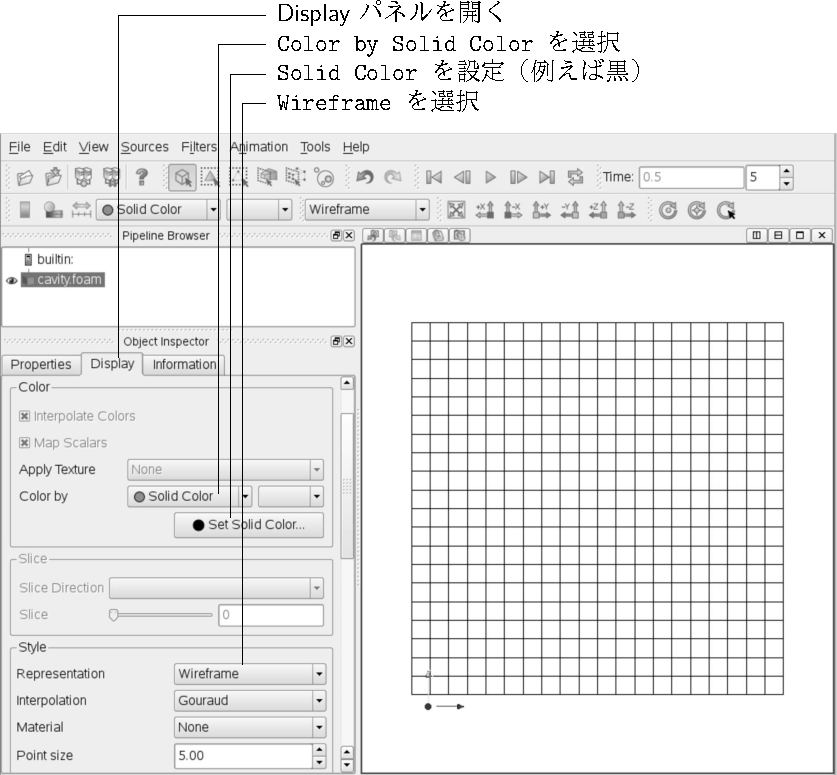
\includegraphics{fig-2-3}
 \caption{paraFoamでのメッシュの表示}
 \label{fig:2.3}
\end{figure}


\OFthirdparty{ParaView}を使うのがはじめてならば,
\autoref{ssec:6.1.5}で述べるように視点操作を試してみることをお勧めします.
特に本ケースは2次元なので\PVkeyword{Edit}メニューの
\index{View Settings@\PVkeyword{View Settings}!メニューエントリ}%
\index{メニューエントリ!View Settings@\PVkeyword{View Settings}}%
\PVkeyword{View Settings}のGeneralパネルで
\index{Use Parallel Projection@\PVbutton{Use Parallel Projection}!ボタン}%
\index{ボタン!Use Parallel Projection@\PVbutton{Use Parallel Projection}}%
\PVbutton{Use Parallel Projection}を
選択するのがよいでしょう.
軸の方向は,
\index{Annotation@\PVpanel{Annotation}!ウィンドウパネル}%
\index{ウィンドウパネル!Annotation@\PVpanel{Annotation}}%
\PVpanel{Annotation}ウィンドウの
\index{Orientation Axes@\PVbutton{Orientation Axes}!ボタン}%
\index{ボタン!Orientation Axes@\PVbutton{Orientation Axes}}%
\PVbutton{Orientation Axes}をオン・オフするか,
マウスのドラッグ\&ドロップによって操作することができます.


\subsection{アプリケーションの実行}
\label{ssec:2.1.3}
あらゆるUNIX/Linuxの実行ファイルと同様に,
OpenFOAMアプリケーションは二つの方法で実行することができます.
一つ目は
\index{フォアグラウンド!プロセス}%
\index{プロセス!フォアグラウンド}%
フォアグラウンドのプロセスで,
コマンドプロンプトを与えるのにシェルが命令終了まで待つものです.
二つ目は
\index{バックグラウンド!プロセス}%
\index{プロセス!バックグラウンド}%
バックグラウンドプロセスで,
シェルがさらなる命令を受け入れるのに命令完了の必要がないものです.

ここでは,フォアグランドで
\index{icoFoam@\OFtool{icoFoam}!ソルバ}%
\index{ソルバ!icoFoam@\OFtool{icoFoam}}%
\OFtool{icoFoam}を動かしましょう.
\OFtool{icoFoam}ソルバはケースディレクトリ内に入って,
コマンドプロンプト上で
\begin{OFverbatim}[terminal]
icoFoam
\end{OFverbatim}
と入力することで実行できますが,

あるいはオプションに\texttt{-case}をつけることで
他のディレクトリからでも起動することができます.
\begin{OFverbatim}[terminal]
icoFoam -case $FOAM_RUN/tutorials/incompressible/icoFoam/cavity
\end{OFverbatim}%$
ジョブの進行過程は,ターミナルウィンドウに表示されます.
現在の時刻,最大Courant数,全てのフィールドの初期値と最終的結果を表示します.


\subsection{後処理}
\label{ssec:2.1.4}
結果が時刻ディレクトリに書かれるとすぐに,
\OFtool{paraFoam}を使って見ることができます.
\OFtool{para\-Foam}ウィンドウに戻って,
\texttt{cavity.OpenFOAM}ケースモジュールの
\index{Properties@\PVpanel{Properties}!ウィンドウパネル}%
\index{ウィンドウパネル!Properties@\PVpanel{Properties}}%
\PVpanel{Properties}パネルを選択してください.
ケースモジュールのパネルが存在していないようならば,
\texttt{cavity.OpenFOAM}が青くハイライトされているか,
それと並んだ目のボタンは表示が有効であることを示しているか,
を確認してください.

見たいデータを表示する\OFtool{paraFoam}を準備するには,
最初に必須の実行時間として$0.5\unit{s}$分のデータを読込まなければなりません.
ケースが実行中で一方\OFthirdparty{ParaView}を開いている場合,
時間ディレクトリの出力データは\OFthirdparty{ParaView}に自動的にロードはされません.
データをロードするためには,\PVwindow{Properties}ウィンドウで
\index{Refresh Times@\PVbutton{Refresh Times}!ボタン}%
\index{ボタン!Refresh Times@\PVbutton{Refresh Times}}%
\PVbutton{Refresh Times}をクリックします.
これで各時刻のデータが\OFthirdparty{ParaView}にロードされます.

\subsubsection{等値面とコンタプロット}
\label{sssec:2.1.4.1}
圧力を見るには
\index{Display@\PVpanel{Display}!ウィンドウパネル}%
\index{ウィンドウパネル!Display@\PVpanel{Display}}%
\PVpanel{Display}パネルを開き,
選択したモジュールの表示形式を調整します.
圧力分布を見るには\autoref{fig:2.4}に示すように
\PVpanel{Style}パネルのRepresentationメニューをsurfaceにして
ColorPanelのSet Color byを 
\includegraphics{icon-point-p},
そして
\index{Rescale to Data Range@\PVbutton{Rescale to Data Range}!ボタン}%
\index{ボタン!Rescale to Data Range@\PVbutton{Rescale to Data Range}}%
\PVbutton{Rescale to Data Range}ボタンをクリックし,
メニューバーの下のツールバーにある
\index{VCR Controls@\PVkeyword{VCR Controls}!メニュー}%
\index{メニュー!VCR Controls@\PVkeyword{VCR Controls}}%
\PVkeyword{VCR Controls}または
\index{Current Time Controls@\PVkeyword{Current Time Controls}!メニュー}%
\index{メニュー!Current Time Controls@\PVkeyword{Current Time Controls}}%
\PVkeyword{Current Time Controls}で現在時刻を0.5にして$t = 0.5\unit{s}$における解析結果を表示します.
それらのパネルは\autoref{fig:6.4}に示すように
\OFthirdparty{ParaView}ウィンドウのトップメニューの下にあります.
圧力場の解析結果は\autoref{fig:2.5}のように左上が低く,
右上が高い圧力分布になるはずです.

圧力分布を作成するには\autoref{fig:2.4}に示すように
StylePanelでRepresentationメニューからSurfaceを選択し,
Colorパネルで 
\includegraphics{icon-point-p},
そしてRescale to Data RangeボタンによってColorを選択します.
メニューバーの下のツールバーにあるVCR Controlsまたは
Current timeを0.5にして$t = 0.5\unit{s}$における解析結果を表示します.


\includegraphics{icon-point-p} のアイコンで圧力分布をセル間を補完した連続分布を表示します.
もしColor byメニューからセルアイコン 
\includegraphics{icon-cell-p} を選択しなければ
各々のセルが等級づけなしで一つの色によって意味されるように,
圧力のための一つの値は各々のセルに起因しています.

Active Variable Controlsツールバーの
Toggle Color Legend Visibilityボタンをクリックするか
\PVkeyword{View}メニューから
\index{Show Color Legend@\PVkeyword{Show Color Legend}!メニューエントリ}%
\index{メニューエントリ!Show Color Legend@\PVkeyword{Show Color Legend}}%
\PVkeyword{Show Color Legend}を選択することで,
カラーバーを表示させることができます.
Active Variable Controls toolbarか\PVpanel{Display}ウィンドウの
Color panelにあるEdit Color Map buttonをクリックすると
フォントの大きさや種類,スケールの番号付けの形式など,
カラーバーの設定を変更することができます.
カラーバーはドラッグアンドドロップによりimageウィンドウに置くことも可能です.

最近のバージョンの\OFthirdparty{ParaView}では,
よく使われる青・緑・赤という(虹色の)カラースケールではなく,
青から白そして赤へと変化するカラースケールがデフォルトになっています.
そこで,はじめて\OFthirdparty{ParaView}を使うユーザはこのカラースケールを変えたいと思うでしょう.
これは,\PVwindow{Color Scale Editor}で\PVbutton{Choose Preset}を選び,
\PVentry{Blue to Red Rainbow}を選択することで変更できます.
\PVbutton{OK}ボタンで確定したあとに,\PVbutton{Make Default}を押せば
\OFthirdparty{ParaView}はいつもこのタイプのカラーバーを使うようになります.

イメージを回転をさせるとすべての表面に圧力分布で色づけされていることが
確認できます.正しいコンタ図を得るために断面を作成するか,
\autoref{sssec:6.1.6.1}に示すsliceフィルタを用いてジオメトリを
スライスします.\autoref{sssec:6.1.6.1}に示すsliceフィルタを用います.
断面の中心座標は$(0.05, 0.05, 0.005)$,
基準点は$(0, 0, 1)$とします (\PVbutton{Z Normal}ボタンをクリックします).
断面を作成後,\autoref{ssec:6.1.6}に示すcontourフィルタによってコンタを描画します.


\begin{figure}[ht]
 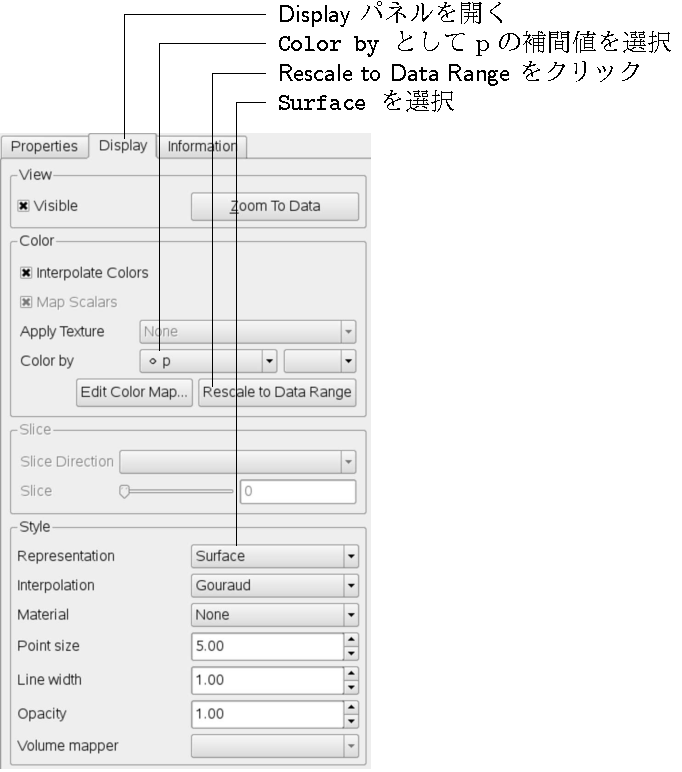
\includegraphics{fig-2-4}
 \caption{キャビティケースでの圧力等圧線の描画}
 \label{fig:2.4}
\end{figure}


\begin{figure}[ht]
 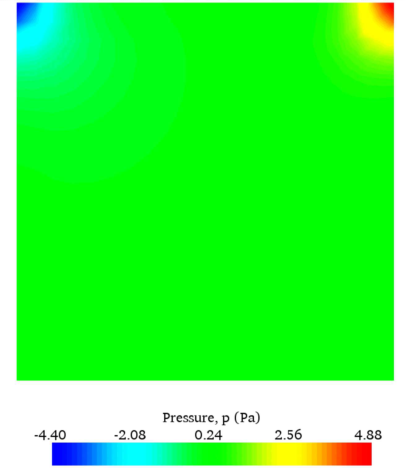
\includegraphics{fig-2-5}
 \caption{キャビティケースでの圧力}
 \label{fig:2.5}
\end{figure}


\subsubsection{ベクトルプロット}
\label{sssec:2.1.4.2}
流速ベクトルを描画する前に,先に作成した断面やコンタなどの
他のモジュールは不要なので取り除きましょう.
\PVwindow{Pipeline Browser}でそれらのモジュールを選択し,
Properties PanelのDeleteをクリックして削除するか,
\PVwindow{Pipeline Browser}で目の形のボタンをクリックして
それらのモジュールを非表示にします.

各格子の中心におけるベクトルグラフを作成することにしましょう.
まず,\autoref{sssec:6.1.7.1}に述べるように
格子の中心のデータのみに絞り込みます.
\PVwindow{Pipeline Browser}上で強調表示されている
cavity.OpenFOAMのモジュールを選択し,
Filter $\rightarrow$ AlphabeticalメニューからCell Centersを選択してApplyをクリックします.

\PVwindow{Pipeline Browser}でCentersが強調表示された状態で,
Filter $\rightarrow$ AlphabeticalメニューからGlyphを選択します.
\autoref{fig:2.6}のような\PVpanel{Properties}ウィンドウが表示されます.
この\PVpanel{Properties}パネルの\PVkeyword{vectors}メニューでは,
ベクトル場は速度のみなので,速度場\OFkeyword{U}が自動的に選択されています.
\PVkeyword{Scale Mode}は速度の\PVkeyword{Vector Magnitude}が初期値として選択されていますが,
領域全体を通る速度の様子を見るために,\PVkeyword{off}を選択し,
\PVentry{Set Scale Factor}に0.005をにします.
\PVbutton{Apply}をクリックするとベクトルが表示されますが,単色,例えば白になっているでしょう.
通常は\PVpanel{Display}パネルで\PVkeyword{Color by U}を選択して速度に応じた色付けをします.
\PVkeyword{Edit Color Map}の中で\PVentry{Show Color Legend}を選択し,
速度の凡例を表示させましょう.出力結果は\autoref{fig:2.7}のようになります.
\index{Color Legend@\PVwindow{Color Legend}!ウィンドウ}%
\index{ウィンドウ!Color Legend@\PVwindow{Color Legend}}%
\PVwindow{Color Legend}(凡例)にはTimes Romanフォントが使用され,
\PVentry{Automatic Label Format}を解除して\PVentry{Label Format}テキストボックスに
\verb|%-#6.2f|を入力することで二つの有効数字でラベルを固定しています.
背景色は,\autoref{sssec:6.1.5.1}で述べるように,
\PVkeyword{View Settings}の\PVpanel{General}パネルで白に設定されています.

左右の壁において,ベトルが壁面を通り抜けるように見えていることに注意してください.
しかし,さらによく調べると,この壁に垂直な方向を向いている速度は$0$であることがわかります.
この少し混乱する状態は,スケーリングが\PVkeyword{off}で速度が$0$のとき,
\OFthirdparty{ParaView}は$x$方向のベクトルで表示するということに起因します.


\begin{figure}[ht]
 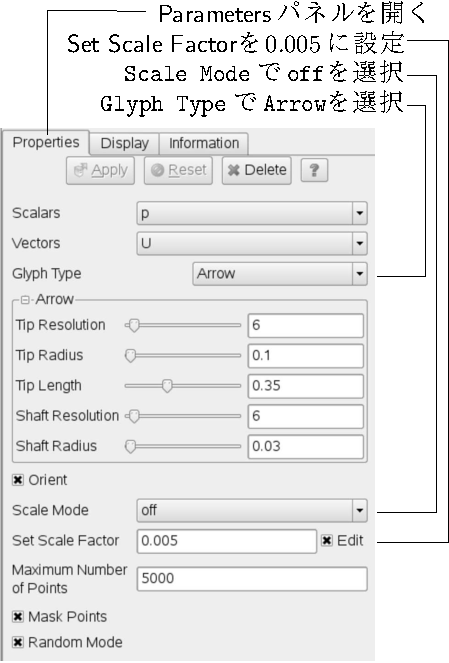
\includegraphics{fig-2-6}
 \caption{Glyphフィルタのパラメータパネル}
 \label{fig:2.6}
\end{figure}


\begin{figure}[ht]
 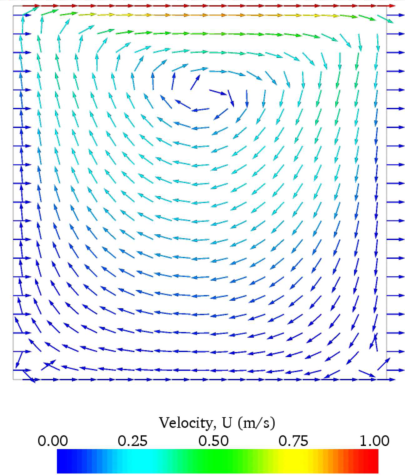
\includegraphics{fig-2-7}
 \caption{キャビティケースの速度}
 \label{fig:2.7}
\end{figure}


\subsubsection{流線プロット}
\label{sssec:2.1.4.3}
\OFthirdparty{ParaView}で後処理を続ける前に,
上述のベクトルプロットのモジュールは不要なので削除しましょう.
そうしたら,\autoref{ssec:6.1.8}の記述のように流速の流線をプロットしましょう.

\PVwindow{Pipeline Browser}で\texttt{cavity.OpenFOAM}モジュールをハイライトした状態で,
\PVmenu{Filter}メニューから\PVfilter{Stream Tracer}を選択し,\PVbutton{Apply}をクリックします.
そうすると,\autoref{fig:2.8}に示すように
\PVpanel{Propaties}ウィンドウが現れます.
\PVentry{Seed}の点は,ジオメトリの中心を垂直に通って,
\PVkeyword{Line Sourse}に沿うように (例えば$(0.05, 0, 0.005)$から
$(0.05, 0.1, 0.005)$まで) 指定しましょう.
このガイドに掲載した図では\PVentry{Point Resolution}を21に,
\PVentry{Max Propagation}を\PVkeyword{Length}で0.5に,
\PVentry{Initial Step Length}を\PVkeyword{Cell Length}で0.01に,
\PVentry{Integration Direction}を\PVkeyword{BOTH}という設定を行いました.
また,\PVkeyword{Runge--Kutta 2} \PVentry{Integrator Type}は
デフォルトパラメータで使いました.

\PVbutton{Apply}をクリックすると,トレーサが生成されます.
そこで\PVmenu{Filter}メニューから\PVkeyword{Tubes}を選択することで,
高品質の流線図を作ることができます.
このレポートでは,次の設定を使いました.
\PVentry{Num.\ sides}を20,\PVentry{Radius}を0.003,\PVentry{Radius factor}を10にしました.
\PVbutton{Accept}を押すことで,\autoref{fig:2.9}ができます.


\begin{figure}[ht]
 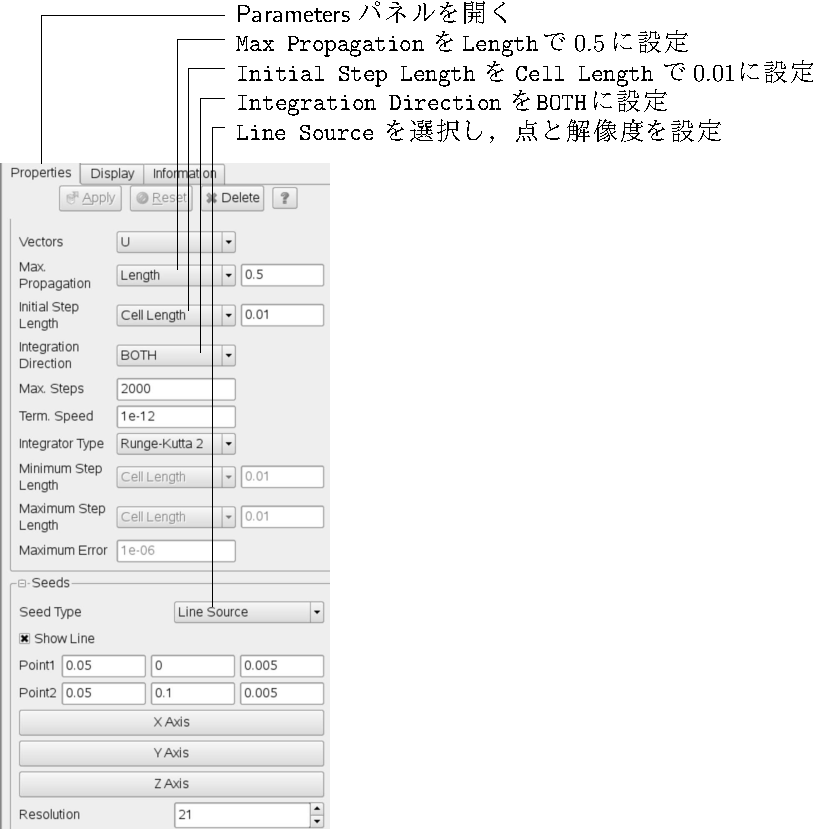
\includegraphics{fig-2-8}
 \caption{Stream Tracerフィルタのパラメータパネル}
 \label{fig:2.8}
\end{figure}


\begin{figure}[ht]
 \includegraphics{fig-2-9}
 \caption{キャビティケースの流線}
 \label{fig:2.9}
\end{figure}


\subsection{メッシュの解像度を増やす}
\label{ssec:2.1.5}
\index{メッシュ!かいぞうど@解像度}%
メッシュの解像度を各々の方向で2倍に増やします.
問題の初期条件として使うために,
粗いメッシュでの結果を,細かいメッシュ上に写像します.
そして,細かいメッシュの解を粗いメッシュの解と比較します.

\subsubsection{既存ケースを用いた新しいケースの作成}
\label{sssec:2.1.5.1}
\OFcase{cavity}をコピーし,
修正することで解析ケース\OFcase{cavityFine}を作成します.
まず\OFpath{cavity}と同じ階層に新しいディレクトリを作成します.
\begin{OFverbatim}[terminal]
cd $FOAM_RUN/tutorials/incompressible/icoFoam
mkdir cavityFine
\end{OFverbatim}%$
基本となる解析ケース\OFpath{cavity}の内容を
解析ケース\OFpath{cavityFine}にコピーし,
\OFpath{cavityFine}に移動します.
\begin{OFverbatim}[terminal]
cp -r cavity/constant cavityFine
cp -r cavity/system cavityFine
cd cavityFine
\end{OFverbatim}

\subsubsection{細かいメッシュの作成}
\label{sssec:2.1.5.2}
\OFtool{blockMesh}を使って計算格子数を増やしましょう.
\OFdictionary{blockMeshDict}ファイルをエディタで開き,
ブロックに関する記述を修正します.
ブロックを特定するには
\index{blocks@\OFkeyword{blocks}!キーワード}%
\index{キーワード!blocks@\OFkeyword{blocks}}%
\OFkeyword{blocks}というキーワードを用いましょう.
ブロック定義の対称性に関しては\autoref{sssec:5.3.1.3}で詳しく述べるので,
ここではhexが最初の頂点リストで,
各方向の計算格子の番号リストがあることを知ればよいでしょう.
これは,先の\OFcase{cavity}ケースでは\texttt{(20 20 1)}になっています.
これを\texttt{(40 40 1)}に変え,保存します.
ここで\OFtool{blockMesh}を実効することで新しい,
より細かいメッシュを生成することができます.

\subsubsection{粗いメッシュの結果を細かなメッシュにマッピングする}
\label{sssec:2.1.5.3}
\index{mapFields@\OFtool{mapFields}!ユーティリティ}%
\index{ユーティリティ!mapFields@\OFtool{mapFields}}%
\OFtool{mapFields}ユーティリティは,他のジオメトリの対応するフィールドの上へ
与えられたジオメトリに関した一つ以上のフィールドをマッピングします.
本チュートリアルの例では,入力フィールドと求める結果のフィールド両方の
ジオメトリ・境界の種類・境界条件が同一であるので,
フィールドは『首尾一貫している』と考えられます.
この例で\OFtool{mapFields}を実行するとき,
\texttt{-consistent}コマンドラインオプションを使います.

mapFields mapsのフィールドデータは,
目的ケース(すなわち結果が図にされている)の
\index{controlDict@\OFdictionary{controlDict}!ディクショナリ}%
\index{ディクショナリ!controlDict@\OFdictionary{controlDict}}%
\OFdictionary{controlDict}内の
startFrom/startTimeで指定される時間ディレクトリから読まれます.
この例では,\OFcase{cavityFine}ケースの細かいメッシュ上に\OFcase{cavity}ケースから
粗いメッシュの最終結果をマッピングしましょう.
これらの結果が\OFpath{cavity}の\OFpath{0.5}のディレクトリに格納されているので,
startTimeを\OFdictionary{controlDict}ディクショナリで$0.5\unit{s}$に,
startFromをstartTimeにセットします.これらの変更を保存しましょう.

\OFtool{mapFields}を実行する準備ができました.
\texttt{mapFields -help}と打ち込むと\OFtool{mapFields}の実行には入力ケースの
ディレクトリを指定する必要があることがわかります.
\texttt{-consistent}オプションを使うので,
次のようにユーティリティは\OFpath{cavityFine}ディレクトリから実行される.
\begin{OFverbatim}[terminal]
mapFields ../cavity -consistent
\end{OFverbatim}
\OFtool{mapFields}が実行され次のように出力されるでしょう.
\begin{OFverbatim}[baselinestretch=0.8, weight=\small]
Source: ".." "cavity"
Target: "." "cavityFine"

Create databases as time

Source time: 0.5
Target time: 0.5
Create meshes

Source mesh size: 400   Target mesh size: 1600

Consistently creating and mapping fields for time 0.5

    interpolating p
    interpolating U

End
\end{OFverbatim}

\subsubsection{設定の調整}
\label{sssec:2.1.5.4}
さて,全てのセルの寸法が半分になったので,
$1$より小さいCourant数を維持するためには\autoref{sssec:2.1.1.4}で述べるように
時間ステップを半分にしなければいけません.
deltaTを\OFdictionary{controlDict}ディクショナリにて$0.0025\unit{s}$に設定しましょう.
いままでは,フィールドデータを固定のステップ回数のもとでの時間間隔で
出力する方法を示してきましたが,
今回は固定の計算時間でデータ出力を指定する方法を示してみましょう.
\OFdictionary{controlDict}の\OFkeyword{writeControl}キーワード下において,
\index{timeStep@\OFkeyword{timeStep}!キーワードエントリ}%
\index{キーワードエントリ!timeStep@\OFkeyword{timeStep}}%
\OFkeyword{timeStep}エントリで固定のステップ回数で出力する代わりに,
\index{runTime@\OFkeyword{runTime}!キーワードエントリ}%
\index{キーワードエントリ!runTime@\OFkeyword{runTime}}%
\OFkeyword{runTime}を使って固定の計算時間を指定して結果を出力することができます.

このケースでは0.1ごとの出力を指定します.
したがって,\OFkeyword{writeControl}を\OFkeyword{runTime}に,
\index{writeInterval@\OFkeyword{writeInterval}!キーワード}%
\index{キーワード!writeInterval@\OFkeyword{writeInterval}}%
\OFkeyword{writeInterval}を0.1に設定しましょう.このようにすることで,
ケースは粗いメッシュでの解を入力条件として計算をはじめるので,
定常状態に収束するには適切な短い時間だけ動かせばよいのです.
したがって,\OFkeyword{endTime}は$0.7\unit{s}$でよいでしょう.
これらの設定が正しいことを確認し,ケースを保存しましょう.

\subsubsection{バックグラウンドプロセスとしてコードを動かす}
\label{sssec:2.1.5.5}
\OFtool{icoForm}をバックグラウンドプロセスとして動かしてみて,
最終的な結果を後で見ることができるように\OFpath{log}ファイルに出力しましょう.
\OFpath{cavitiyFine}ディレクトリにおいて次のコマンドを実行してください.
\begin{OFverbatim}[terminal]
icoFoam > log &
cat log
\end{OFverbatim}

\subsubsection{精密なメッシュによるベクトルプロット}
\label{sssec:2.1.5.6}
各々の新しいケースは本質的には単なるPipeline Browserに現れる
他のモジュールであるので,
\OFthirdparty{ParaView}で同時に複数のケースを開くことができます.
若干不便なことには,\OFthirdparty{ParaView}で新しいケースを開けるときには,
選ばれたデータが拡張子を含むファイル名である必要があります.
しかし,OpenFOAMにおいて,
各々のケースは特定のディレクトリ構造の中に拡張子なしで
複数のファイルに保存されます.
解決方法として,\OFtool{paraFoam}スクリプトが自動的に拡張子
\OFpath{.OpenFOAM}が付いたダミーファイルを作成することになっています.
それゆえに,\OFcase{cavity}ケースモジュールは
\texttt{cavity.OpenFOAM}と名づけられます.

\OFthirdparty{ParaView}内から他のケースディレクトリを開けたいならば,
そのようなダミーファイルを作成する必要があります.
たとえば,\OFcase{cavityFine}ケースを読み込むには,
コマンドプロンプトで次のようにタイプしてファイルを作成します.
\begin{OFverbatim}[terminal]
cd $FOAM_RUN/tutorials/incompressible/icoFoam
touch cavityFine/cavityFine.OpenFOAM
\end{OFverbatim}%$

こうしてFileメニューからOpen Dataを選んでディレクトリツリーをたどり,\break
\texttt{cavityFine.OpenFOAM}を選ぶことで,
cavityFineケースを\OFthirdparty{ParaView}に読み込めるようになりました.
さて,\OFthirdparty{ParaView}で精密なメッシュの結果の
ベクトルプロットを作ることができます.
同時に両方のケースのglyphを見られるようににすることによって,
\OFcase{cavityFine}ケースのプロットを\OFcase{cavity}ケースと比較することができます.


\begin{figure}[ht]
 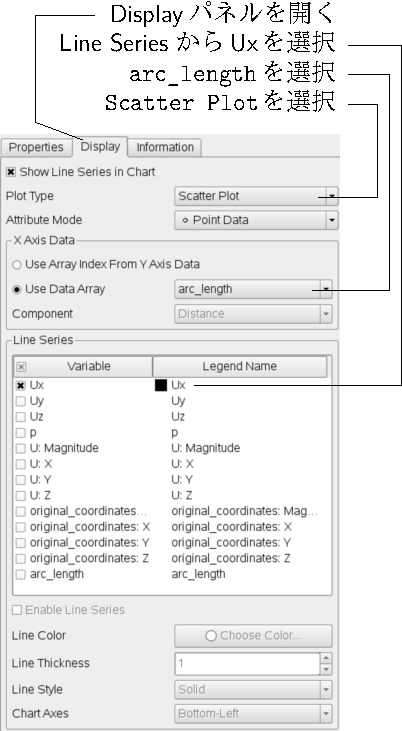
\includegraphics{fig-2-10}
 \caption{グラフ作図のためのフィールド選択}
 \label{fig:2.10}
\end{figure}


\subsubsection{グラフを描く}
\label{sssec:2.1.5.7}
OpenFOAMは,速度のスカラ値を抽出して2次元のグラフに
描画したい場合のデータの取り扱いに長けています.
データを操作するための特別なユーティリティが多数あり,
単純な計算を
\index{foamCalc@\OFtool{foamCalc}!ユーティリティ}%
\index{ユーティリティ!foamCalc@\OFtool{foamCalc}}%
\OFtool{foamCalc}によって組み合わせることができます.
次のようにユーティリティを指定して実行します.
\begin{OFverbatim}[terminal]
foamCalc <calcType> <fieldName1 ... fieldNameN>
\end{OFverbatim}
処理を規定する\texttt{<calcType>}には\texttt{addSubtract},
\texttt{randomise},\texttt{div},\texttt{components},\texttt{mag},
\texttt{magGrad},\texttt{magSqr},\texttt{interpolate}を指定することができます.
\texttt{<calcType>}のリストを見るには,
意図的に無効な処理を要求することでエラーメッセージとともに見ることができます.
\begin{OFverbatim}[baselinestretch=0.8, weight=\small]
>> foamCalc xxxx
Selecting calcType xxxx
unknown calcType type xxxx, constructor not in hash table
Valid calcType selections are:

8
(
randomise
magSqr
magGrad
addSubtract
div
mag
interpolate
components
)
\end{OFverbatim}

\OFkeyword{components}および\OFkeyword{mag}の\OFkeyword{calcType}はスカラ速度を計測するのに有用です.
ケースにて ``\texttt{foamCalc components U}'' を動かすと,
各時刻のディレクトリから速度のベクトル場を読み込み,
各ディレクトリに各軸方向成分のスカラ場
\OFkeyword{Ux},\OFkeyword{Uy},\OFkeyword{Uz}を書き出します.
同様に ``\texttt{foamCalc mag U}'' とは各時刻のディレクトリに
スカラ場\OFkeyword{magU}を書き込みます.

\OFtool{foamCalc}は\OFcase{cavity}と
\OFcase{cavityFine}のどちらに対しても実行することができます.
例えば\OFcase{cavity}に対しては,
以下のように\OFpath{cavity}ディレクトリに移動して\OFtool{foamCalc}を実行します.
\begin{OFverbatim}[terminal]
cd $FOAM_RUN/tutorials/incompressible/icoFoam/cavity
foamCalc components U
\end{OFverbatim}%$
それぞれの成分が\OFthirdparty{ParaView}内でグラフとして描画されます.
簡単に,早く,しかもラベル付けや形式化の調整ができるので,
とても高性能な出力を表示ができます.
しかしながら,出版用にグラフを作成するならばgnuplotやGrace/xmgrなどの
専用のグラフ描画ソフトを使って生データから作画するのがよいでしょう.
これを行うには,\autoref{sec:6.5}や\autoref{ssec:2.2.3}で述べる
\OFtool{sample}ユーティリティを使うとよいでしょう.

描画をする前に,新しく生成された\OFkeyword{Ux},\OFkeyword{Uy},\OFkeyword{Uz}のデータを
\OFthirdparty{ParaView}に読み込ませる必要があります.
これには,\texttt{cavity.OpenFOAM}モジュールのPropertiesパネルの上部にある
Refresh Timesをクリックします.
これにより,\OFthirdparty{ParaView}に新しいフィールドが読み込まれ,
Volume Fieldsウィンドウに現れます.
新しいフィールドを選択し,変更が適用されたことを確認します.
つまり,必要ならApplyを再度クリックします.
また,Mesh Partsパネルで境界領域が選択されているならば,
境界部分のデータ補間が不適切に行われています.
したがって,Mesh Partsパネルで,
\OFpatch{movingwall}や\OFpatch{fixedwall},\OFpatch{frontAndBack}といった
パッチの選択を解除して,変更を適用します.

さて,\OFthirdparty{ParaView}でグラフを表示してみましょう.
まずは描画したいモジュールを選択し,
\index{Plot Over Line@\PVfilter{Plot Over Line}!メニューエントリ}%
\index{メニューエントリ!Plot Over Line@\PVfilter{Plot Over Line}}%
\PVfilter{Plot Over Line}フィルタを\PVmenu{Filter} $\rightarrow$ \PVmenu{Data Analisys}から選択します.
\PVwindow{3D View}ウィンドウの下または横に新しい\PVwindow{XY Plot}ウィンドウが開きます.
\PVpanel{Properties}ウィンドウで線の終点を指定すると
Plobelineモジュールが作成されます.
この例ではPoint1を$(0.05, 0, 0.005)$,
Point2を$(0.05, 0.1, 0.005)$と指定して線を領域の中心の真上におきます.
Resolutionは100まで設定できます.

\PVbutton{Apply}をクリックすると\PVwindow{XY Plot}ウィンドウにグラフが描画されます.
\PVpanel{Display}パネルで,
\index{Attribute Mode@\PVmenu{Attribute Mode}!メニュー}%
\index{メニュー!Attribute Mode@\PVmenu{Attribute Mode}}%
\PVmenu{Attribute Mode}を\PVkeyword{Point Data}に設定します.
\PVkeyword{Use Data Array}オプションを\PVkeyword{X Axis Data}にし,
\verb|arc_length|オプションを加えて,
グラフの$x$軸データがキャビティの底からの距離になるようにできます.

\PVpanel{Display}ウィンドウの\PVpanel{Line Series}パネルから
表示するデータを選択することができます.
表示されているスカラ場のリストから,
ベクトルの大きさや成分を初期値とすることもできます.
つまり,\OFkeyword{Ux}を\OFtool{foamCalc}から計算する必要はありません.
それでも,\OFkeyword{Ux}以外の系列の選択はすべて解除しましょう.
選択した系列の上の四角形の色が線の色です.
この上でダブルクリックをすれば簡単に変更することができます.

グラフの体裁を整えるには,\PVpanel{Line Series}パネルの下にある設定,
\PVkeyword{Line Color},\PVkeyword{Line Thickness},\PVkeyword{Line Style},
\PVkeyword{Marker Style},そして\PVkeyword{Chart Axes}を変更します.

また,\PVwindow{XY Plot}の左上にあるボタンをクリックすることもできます.
例えば,3番目のボタンでは,それぞれの軸のタイトルや凡例などを設定する
\PVentry{View Settings}を制御することができます.
また,軸のタイトルのフォント,色,配置,
値の範囲や線形・対数表示など,様々な設定を行うことができます.

\autoref{fig:2.11}は\OFthirdparty{ParaView}によって作画された図です.
望みどおりのグラフが作成できます.
\autoref{fig:2.11}は軸のオプションとして
Standard type of Notation,Specify Axis Rangeを選択し,
フォントはSans Serifの12ポイントです.
このグラフは点で表示していますが,
\PVpanel{Display}ウィンドウで
\index{Enable Line Series@\PVbutton{Enable Line Series}!ボタン}%
\index{ボタン!Enable Line Series@\PVbutton{Enable Line Series}}%
\PVbutton{Enable Line Series}ボタンを
有効にすれば線で表示できます.
注:もしこのボタンが,グレー表示で無効の状態になっていたら,
\PVpanel{Line Series}パネルでどれか変数を選択すれば有効になります.
\PVbutton{Enable Line Series}ボタンを選択しておけば,
\index{Line Style@\PVmenu{Line Style}!メニュー}%
\index{メニュー!Line Style@\PVmenu{Line Style}}%
\PVmenu{Line Style}や
\index{Marker Style@\PVmenu{Marker Style}!メニュー}%
\index{メニュー!Marker Style@\PVmenu{Marker Style}}%
\PVmenu{Marker Style}もユーザの好みで調整できます.


\begin{figure}[ht]
 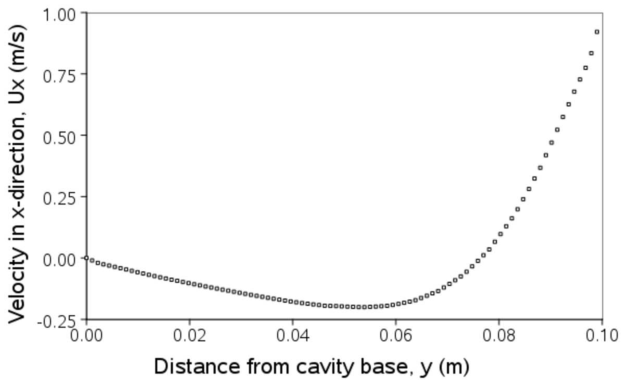
\includegraphics{fig-2-11}
 \caption{\OFtool{paraFoam}でのグラフ作図}
 \label{fig:2.11}
\end{figure}


\subsection{勾配メッシュ}
\label{ssec:2.1.6}
解の誤差は,正しい解の形と選択した数値スキームで想定される形とが
大きく異なる領域で出ます.
例えば,数セルにわたる変数の線形変化に基づく数値スキームは,
正しい解自体が線形の場合にしか正確な解を導くことができません.
例えば勾配の変化が最も大きいところのような正しい解が
線形から一番大きく外れる領域で誤差は最も大きくなります.
セルの大きさに従って,誤差は減少します.

どんな問題も取りかかる前に解の概形の直感的予測ができるといいです.
次に,誤差が最も大きくなるところを予測し,メッシュ幅に勾配をつけ,
最も小さいセルがこれらの領域にくるようにします.
キャビティの場合,壁の近くで速度の大きい変化があることを予想できるので,
チュートリアルのこの部分では,メッシュがこの領域で,
より小さくなるように勾配付けします.
同じ数のセルを使用することによって,
コンピュータの負荷をあまり増加させずに,より精度を上げられます.

lid-drivenキャビティ問題のために壁に向かって勾配を付けた
$20 \times 20$セルのメッシュを作り,
\autoref{sssec:2.1.5.2}の細かいメッシュの結果を初期条件として
勾配付けされたメッシュに適用しましょう.
そして,勾配付けされたメッシュの結果を前のメッシュの結果と
比較してみましょう.
\index{blockMeshDict@\OFdictionary{blockMeshDict}!ディクショナリ}%
\index{ディクショナリ!blockMeshDict@\OFdictionary{blockMeshDict}}%
\OFdictionary{blockMeshDict}ディクショナリの書換えはとても重要であるので,
チュートリアルのこの部分を使ったケース (\OFpath{cavityGrade}) は
\OFpath{\$FOAM\_RUN/tutorials/incompressible/icoFoam}ディレクトリに入れておきました.

\subsubsection{勾配メッシュの作成}
\label{sssec:2.1.6.1}
ここで,四つの異なるメッシュ間隔の計算メッシュが計算領域の
上下左右のブロックに必要となります.
このメッシュのブロック構造を\autoref{fig:2.12}に示します.


\begin{figure}[ht]
 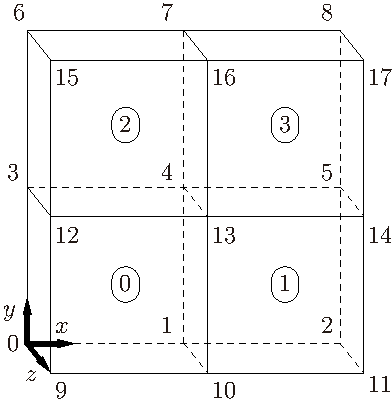
\includegraphics{fig-2-12}
 \caption{キャビティケースの勾配メッシュのブロック構造(ブロック番号)}
 \label{fig:2.12}
\end{figure}


\OFpath{cavityGrade}の\OFpath{constant/polyMesh}サブディレクトリで
\OFdictionary{blockMeshDict}ファイルを見ることができます.
念のため\OFdictionary{blockMeshDict}の重要な要素を以下に述べます.
それぞれのブロックは$x$方向,$y$方向に10セルを有し,
もっとも大きなセルともっとも小さなセルとの大きさの比は2です.
\begin{OFverbatim}[file, linenum=17]
/*--------------------------------*- C++ -*----------------------------------*\
| =========                 |                                                 |
| \\      /  F ield         | OpenFOAM: The Open Source CFD Toolbox           |
|  \\    /   O peration     | Version:  2.3.0                                 |
|   \\  /    A nd           | Web:      www.OpenFOAM.com                      |
|    \\/     M anipulation  |                                                 |
\*---------------------------------------------------------------------------*/
FoamFile
{
    version     2.0;
    format      ascii;
    class       dictionary;
    object      blockMeshDict;
}
// * * * * * * * * * * * * * * * * * * * * * * * * * * * * * * * * * * * * * //

convertToMeters 0.1;

vertices        
(
    (0 0 0)
    (0.5 0 0)
    (1 0 0)
    (0 0.5 0)
    (0.5 0.5 0)
    (1 0.5 0)
    (0 1 0)
    (0.5 1 0)
    (1 1 0)
    (0 0 0.1)
    (0.5 0 0.1)
    (1 0 0.1)
    (0 0.5 0.1)
    (0.5 0.5 0.1)
    (1 0.5 0.1)
    (0 1 0.1)
    (0.5 1 0.1)
    (1 1 0.1)
);

blocks          
(
    hex (0 1 4 3 9 10 13 12) (10 10 1) simpleGrading (2 2 1)
    hex (1 2 5 4 10 11 14 13) (10 10 1) simpleGrading (0.5 2 1)
    hex (3 4 7 6 12 13 16 15) (10 10 1) simpleGrading (2 0.5 1)
    hex (4 5 8 7 13 14 17 16) (10 10 1) simpleGrading (0.5 0.5 1)
);

edges           
(
);

boundary
(
    movingWall
    {
        type wall;
        faces
        (
            (6 15 16 7)
            (7 16 17 8)
        );
    }
    fixedWalls
    {
        type wall;
        faces
        (
            (3 12 15 6)
            (0 9 12 3)
            (0 1 10 9)
            (1 2 11 10)
            (2 5 14 11)
            (5 8 17 14)
        );
    }
    frontAndBack
    {
        type empty;
        faces
        (
            (0 3 4 1)
            (1 4 5 2)
            (3 6 7 4)
            (4 7 8 5)
            (9 10 13 12)
            (10 11 14 13)
            (12 13 16 15)
            (13 14 17 16)
        );
    }
);

mergePatchPairs
(
);

// ************************************************************************* //
\end{OFverbatim}
いったんこのケースの\OFdictionary{blockMeshDict}ファイルを理解しておけば,
後はコマンドラインから\OFtool{blockMesh}を実行できます.
\autoref{ssec:2.1.2}に示した\OFtool{paraFoam}を使用することで
勾配付けされたメッシュを見ることができます.

\subsubsection{計算時間,時間ステップの変更}
\label{sssec:2.1.6.2}
最も速度が速くて最もサイズの小さいセルが上面に隣接するセルであり,
\autoref{sssec:2.1.1.4}で示したように,
この上面のセルにおいてCourant数が最大となります.
このようなことから上面に隣接するセルの大きさを見積もることは,
本ケースにて適当な時間ステップを計算する上で有効です.

一様でないメッシュ勾配を使用している場合,
\index{blockMesh@\OFtool{blockMesh}!ユーティリティ}%
\index{ユーティリティ!blockMesh@\OFtool{blockMesh}}%
\OFtool{blockMesh}は形状に関する数列をもちいてセルの大きさを算出します.
長さ$l$に沿って,最初と最後のセルとの間に,
比$R$の$n$個の計算セルが必要であるならば,
もっとも小さいセルの大きさは,次のように与えられます.
\begin{align}
 \label{eq:2.5}
  \Delta x_{\mathrm{s}} = l\frac{r - 1}{\alpha r - 1}
\end{align}
ここで,$r$はあるセルの大きさとその隣のセルの大きさとの比であり,
次式で表されます.
\begin{align}
 \label{eq:2.6}
  r = R^{\frac{1}{n-1}}
\end{align}
そして,
\begin{align}
 \label{eq:2.7}
  \alpha =
  \begin{cases}
   R & \text{for}\ R > 1, \\
   1 - r^{-1} + r^{-1} & \text{for}\ R < 1.
  \end{cases}
\end{align}
\OFcase{cavityGrade}ケースにおいては,各方向のセルの数は$10$であり,
最大セルと最小セルとの比は$2$,
ブロックの縦横は$0.05\unit{m}$です.
したがって,最小セルサイズは$3.45\unit{mm}$となります.
\autoref{eq:2.2} から時間ステップは,クラーン数を$1$以下に抑えるために
$3.45\unit{ms}$以下にしなければなりません.
有意な解析結果を得るためには,
時間ステップ\OFkeyword{deltaT}を$2.5\unit{ms}$まで小さくし,
\OFkeyword{writeInterval}を40とします.
これより解析結果は$0.1\unit{s}$ごとに書き出されることとなります.

このように,各設定に対応したファイルを編集することにより,
ケースディクショナリの各種条件を変更することができます.
ここで時間ないし計算経過の書き出しを操作したいならば,
\OFpath{/cavityGrade/system/controlDict}ファイル内に
それらのパラメータは納められており,
任意のエディタでこのファイルを開くことができます.
先に述べたように,計算を収束させるための保証として,
このケースでは時間ステップ\OFkeyword{deltaT}は\texttt{0.25e-3}に,
\OFkeyword{writeInterval}は40とします.

\OFkeyword{startTime}はその\OFcase{cavityFine}ケースの最終的な条件,
すなわち$0.7$に設定される必要があります.
\OFcase{cavity}と\OFcase{cavityFine}が規定された実行時間の中でよく収束させるためには,
\OFcase{cavityGrade}ケースのための実行時間を$0.1\unit{s}$に設定,
すなわち\OFkeyword{endTime}を0.8とします.

\subsubsection{解析場のマッピング}
\label{sssec:2.1.6.3}
\autoref{sssec:2.1.5.3}にあるように
\index{mapFields@\OFtool{mapFields}!ユーティリティ}%
\index{ユーティリティ!mapFields@\OFtool{mapFields}}%
\OFtool{mapFields}を使用して,
\OFcase{cavityFine}ケースの最終的な結果を
\OFcase{cavityGrade}ケースのメッシュにマッピングします.
以下のように\OFpath{cavityGrade}ディレクトリに入り,
\OFtool{mapFields}を実行してください.
\begin{OFverbatim}[terminal]
cd $FOAM_RUN/tutorials/incompressible/icoFoam/cavityGrade
mapFields ../cavityFine -consistent
\end{OFverbatim}%$
今度は,ケースディレクトリから\OFtool{icoFoam}を実行して,
計算実行時の情報をモニタリングします.
そして,\autoref{sssec:2.1.5.6}と\autoref{sssec:2.1.5.7}で説明した
後処理ツールを使って,収束した結果を見たり,他の結果と比較します.


\subsection{Reynolds数の増大}
\label{ssec:2.1.7}
これまで解いたケースはReynolds数が$10$でした.
これは大変に低い条件であり,
したがってキャビティの底部中央に小さな二次渦を伴うのみで,
迅速に安定解を導くことができました.
しかし,ここでReynolds数を$100$に上げると,
収束解を得るのにより長い時間を要することになります.
そこで\OFcase{cavity}ケースのメッシュを初期条件として使用することとします.
\OFpath{cavity}ケースディレクトリを\OFpath{cavityHighRe}という名前でコピーします.
\begin{OFverbatim}[terminal]
cd $FOAM_RUN/tutorials/incompressible/icoFoam
cp -r cavity cavityHighRe
\end{OFverbatim}%$

\subsubsection{後処理}
\label{sssec:2.1.7.1}
\OFpath{cavityHighRe}ケースに入り,
\index{transportProperties@\OFdictionary{transportProperties}!ディクショナリ}%
\index{ディクショナリ!transportProperties@\OFdictionary{transportProperties}}%
\OFdictionary{transportProperties}ディクショナリを編集します.
Reynolds数を10倍に増加させるためには,
動粘性係数を10分の1,すなわち$1 \times 10^{-3} \unit{m^{2}s^{-1}}$まで減らす必要があります.
これで\OFcase{cavity}ケースの実行結果から
\index{リスタート}%
リスタートして,このケースを実行できます.
これを実行するために,\OFkeyword{startFrom}キーワードを
\index{latestTime@\OFkeyword{latestTime}!キーワードエントリ}%
\index{キーワードエントリ!latestTime@\OFkeyword{latestTime}}%
\OFkeyword{latestTime}に
オプションを切り替えることにより,
\OFtool{icoFoam}は,最新の時間ディレクトリを初期データとして使用します(例えば0.5).
\OFkeyword{endTime}は$2\unit{s}$に設定し,本ケースを保存します.

\subsubsection{コードの実行}
\label{sssec:2.1.7.2}
まずはケースディレクトリから\OFtool{icoFoam}を実行し,ランタイム情報を見ます.
バックグラウンドでジョブを実行するときには,以下のUNIXコマンドが便利です.
\begin{description}
 \item[\texttt{nohup}]
            ユーザがログアウト後も稼働し続けるコマンド
 \item[\texttt{nice}]
            カーネル・スケジューラのジョブの優先順位を変えるコマンド.
            $-20$が最優先で,$19$は最も低い優先度.
\end{description}
これらのコマンドは,
例えば,ユーザがリモートマシンでケースを実行できるよう設定し,
頻繁にモニタしなくてもいいような場合,
リモートマシンではケース実行をあまり優先させたくないでしょうが,
そのような場合に便利です.
その場合,ユーザは\texttt{nohup}コマンドで稼働しているリモートマシンを
ログアウトしてジョブを実行し続けることができます.
一方,\texttt{nice}は優先度を19に設定します.
試しに,以下のようにコマンドを実行してみましょう.
\begin{OFverbatim}[terminal]
cd $FOAM_RUN/tutorials/incompressible/icoFoam
nohup nice -n 19 icoFoam > log &
cat log
\end{OFverbatim}%$
お気づきかもしれませんが,前述の解析方法では\OFtool{icoFoam}は,
速度\OFkeyword{U}の計算が止まっても,
それよりもずっと長い間もしくは解析が終わるまで
圧力\OFkeyword{p}の計算をし続けていました.
実際には,\OFtool{icoFoam}がいったん\OFkeyword{U}の計算をやめ,
\OFkeyword{p}の初期残差が\OFdictionary{fvSolution}ディクショナリで
設定された許容値(通常は$10^{-6}$)を下回ると
結果が効率的に収束するので,
フィールド・データをいったん時間ディレクトリに書き出して
計算を止めることができます.
例として,\OFcase{cavityHighRen}ケースの
\index{しゅうそく@収束}%
収束の\OFpath{log}ファイルを以下に示します.
示したとおり,$1.62\unit{s}$後に速度はすでに収束し,
初期の圧力残差は小さくなります.
\OFpath{log}において\verb|No Iterations 0|は,
\OFkeyword{U}の計算が止まったことを示しています.
\begin{OFverbatim}[file, linenum, weight=\scriptsize]
Time = 1.43

Courant Number mean: 0.221921 max: 0.839902
smoothSolver: Solving for Ux, Initial residual = 8.73381e-06, Final residual = 8.73381e-06, No Iterations 0
smoothSolver: Solving for Uy, Initial residual = 9.89679e-06, Final residual = 9.89679e-06, No Iterations 0
DICPCG: Solving for p, Initial residual = 3.67506e-06, Final residual = 8.62986e-07, No Iterations 4
time step continuity errors : sum local = 6.57947e-09, global = -6.6679e-19, cumulative = -6.2539e-18
DICPCG: Solving for p, Initial residual = 2.60898e-06, Final residual = 7.92532e-07, No Iterations 3
time step continuity errors : sum local = 6.26199e-09, global = -1.02984e-18, cumulative = -7.28374e-18
ExecutionTime = 0.37 s ClockTime = 0 s

Time = 1.435

Courant Number mean: 0.221923 max: 0.839903
smoothSolver: Solving for Ux, Initial residual = 8.53935e-06, Final residual = 8.53935e-06, No Iterations 0
smoothSolver: Solving for Uy, Initial residual = 9.71405e-06, Final residual = 9.71405e-06, No Iterations 0
DICPCG: Solving for p, Initial residual = 4.0223e-06, Final residual = 9.89693e-07, No Iterations 3
time step continuity errors : sum local = 8.15199e-09, global = 5.33614e-19, cumulative = -6.75012e-18
DICPCG: Solving for p, Initial residual = 2.38807e-06, Final residual = 8.44595e-07, No Iterations 3
time step continuity errors : sum local = 7.48751e-09, global = -4.42707e-19, cumulative = -7.19283e-18
ExecutionTime = 0.37 s ClockTime = 0 s
\end{OFverbatim}


\subsection{高Reynolds数流れ}
\label{ssec:2.1.8}
では,\OFtool{paraFoam}による結果を確認し,速度ベクトルを表示してください.
計算領域の角における二次渦が幾分増大していることがわかります.
このようなとき,ユーザは粘性係数を下げることにより
Reynolds数を増大させた計算ケースを再度実行できます.
渦の数が増加するにともない,より複雑な流れを解くために
当該領域でのメッシュ解像度を上げる必要がでてきます.
さらに,Reynolds数は収束に要する時間を増加させます.
このような場合,残差をモニタし,解を収束させるために
\OFkeyword{endTime}を延長したほうがよいでしょう.

空間および時間解像度の増加を要することは,
流れが乱流域に移行するという非現実的な状態となり,
解法の安定性の問題が生じることとなります.
もちろん,多くの工学的な問題は
極めて高いReynolds数条件となっており,
したがって,乱流挙動を直接解くのに多くのコストを負担することとなり,
実行不可能であります.
そのかわりに,
\index{らんりゅうモデル@乱流モデル!RAS}%
Reynolds平均シミューレション (RAS) 乱流モデルが
平均流れの挙動を解くのに用いられ,
乱れの統計値が計算されています.
壁関数を伴う標準$k$--$\varepsilon$モデルが
本チュートリアルの上面が移動する
キャビティケース(Reynolds数$10^{4}$)を解くのに用いられています.
二つの追加変数が解かれています.
それは,
\index{らんりゅう@乱流!うんどうエネルギ@運動エネルギ}%
乱流エネルギ$k$,
\index{らんりゅう@乱流!しょうさん@消散}%
乱流消散速度$\varepsilon$です.
乱流のための追加の方程式およびモデルは\OFtool{pisoFoam}と呼ばれる
OpenFOAMソルバにおいて実行されます.

\subsubsection{前処理}
\label{sssec:2.1.8.1}
\OFpath{\$FOAM\_RUN/tutorials/incompressible/pisoFoam/ras}ディレクトリの
\OFpath{cavity}ケースに移動します.
これまでと同様に,\OFtool{blockMesh}を走らせ,
メッシュを生成します.
壁関数付き標準$k$--$\varepsilon$モデルを用いる場合は,
壁近傍のセルにおける流れがモデル化されることにより,
壁方向へのメッシュ勾配は必ずしも必要ではありません.

OpenFOAMでは,様々な壁関数モデルを利用することができ,
それぞれのパッチの境界条件として設定します.
これにより,壁面ごとに異なる壁関数モデルを適用することが可能になります.
壁関数の選択は,乱流粘性係数$\nu_{\mathrm{t}}$の
ファイル\OFpath{0/nut}で指定します.
\begin{OFverbatim}[file, linenum=17]

dimensions      [0 2 -1 0 0 0 0];

internalField   uniform 0;

boundaryField
{
    movingWall
    {
        type            nutkWallFunction;
        value           uniform 0;
    }
    fixedWalls
    {
        type            nutkWallFunction;
        value           uniform 0;
    }
    frontAndBack
    {
        type            empty;
    }
}


// ************************************************************************* //
\end{OFverbatim}
このケースでは標準的な壁関数を採用し,
\OFpatch{movingWall}と\OFpatch{fixedWalls}のパッチに対して
\OFkeyword{nutWall\-Function}タイプを指定しています.
これ以外の壁関数モデルとしては,
粗壁面の壁関数\OFkeyword{nutRough\-WallFunction}などがあります.

次に,$k$と$\varepsilon$のファイル (\OFpath{0/k}と\OFpath{0/epsilon}) を開き,
境界条件を確かめます.
壁タイプの境界条件の選択には,
$\varepsilon$については\OFkeyword{epsilonWallFunction}境界条件を,
$k$については\OFkeyword{kqRWallFunction}を指定します.
後者は乱流運動エネルギの表現$k$,$q$,
あるいはReynolds応力$R$のいずれにも適用できる一般的な壁関数です.
$k$,$\varepsilon$の初期条件には,
速度変動$\bm{U}'$と
\index{らんりゅう@乱流!ながさスケール@長さスケール}%
乱流長さスケール$l$から推測した値を設定します.
$k$と$\varepsilon$は,これらのパラメタを用いて次式で表されます.
\begin{align}
 \label{eq:2.8}
  k &= \frac{1}{2}\overline{\bm{U}' \cdot \bm{U}'} \\
 \label{eq:2.9}
 \varepsilon &= \frac{C_{\mu}^{0.75}k^{1.5}}{l}
\end{align}
ここで$C_{\mu}$は$k$--$\varepsilon$モデルの定数であり,
その値は$0.09$です.Cartesian座標系では$k$は,
\begin{align}
 \label{eq:2.10}
 k = \frac{1}{2}({U_{x}'}^{2} + {U_{y}'}^{2} + {U_{z}'}^{2})
\end{align}
で表されます.各項は$x$,$y$,$z$方向速度乱れ成分です.
ここで,初期乱流が等方的であると仮定します.
例えば,${U_{x}'}^{2} = {U_{y}'}^{2} = {U_{z}'}^{2}$となり,
これら速度は上面速度の$5\unit{\%}$に等しく,
また,乱流長さスケール$l$はボックス幅$0.1\unit{m}$の
$20\unit{\%}$に等しいとすると,次のように表されます.
\begin{align}
 \label{eq:2.11}
 U_{x}' &= U_{y}' = U_{z}' = \frac{5}{100}1\unit{m\,s^{-1}} \\
 \label{eq:2.12}
 \Rightarrow k &= \frac{3}{2}\left(\frac{5}{100}\right)^{2}\unit{m^{2}s^{-2}}
 = 3.75 \times 10^{-3}\unit{m^{2}s^{-2}} \\
 \label{eq:2.13}
 \varepsilon &= \frac{C_{\mu}^{0.75}k^{1.5}}{l}
 \approx 7.65 \times 10^{-4}\unit{m^{2}s^{-3}}
\end{align}
上記のとおり$k$,$\varepsilon$を設定してください.
$U$と$p$に対する初期条件は前と同じように,
それぞれ$(0, 0, 0)$と$0$です.

OpenFOAMで提供されている乱流モデルには,
例えばRASやlarge-edy simulation (LES) のような,
さまざまな手法があります.
ほとんどの非定常ソルバでは,乱流のモデリング手法は
実行時に\OFdictionary{turbulenceProperties}ディクショナリの
\OFkeyword{simulationType}キーワードで選択できます.
このファイルは\OFpath{constant}ディレクトリの中に見つかります.
\begin{OFverbatim}[file, linenum=17]

simulationType  RASModel;


// ************************************************************************* //
\end{OFverbatim}
\OFkeyword{simulationType}の選択肢は
\index{laminar@\OFkeyword{laminar}!キーワードエントリ}%
\index{キーワードエントリ!laminar@\OFkeyword{laminar}}%
\OFkeyword{laminar},
\index{RASModel@\OFkeyword{RASModel}!キーワードエントリ}%
\index{キーワードエントリ!RASModel@\OFkeyword{RASModel}}%
\OFkeyword{RASModel},そして
\index{LESModel@\OFkeyword{LESModel}!キーワードエントリ}%
\index{キーワードエントリ!LESModel@\OFkeyword{LESModel}}%
\OFkeyword{LESModel}です.
このケースで選択されている\OFkeyword{RASModel}の場合,
RASモデリングの選択は
\index{RASProperties@\OFdictionary{RASProperties}!ディクショナリ}%
\index{ディクショナリ!RASProperties@\OFdictionary{RASProperties}}%
\OFpath{RASProperties}ファイルに記述します.
このファイルも同じく\OFpath{constant}ディレクトリにあります.
乱流モデルは\autoref{tbl:3.9}に示されている多くの使用可能なモデルから,
\OFkeyword{RASModel}エントリで選択します.
ここでは,標準$k$--$\varepsilon$モデルである\OFkeyword{kEpsilon}を選択します.
\OFkeyword{turbulence}のスイッチが\OFkeyword{on}になっていることも確認します.
乱流モデルに必要な係数には,それぞれのコードの中でデフォルト値が与えられています.
\index{printCoeffs@\OFkeyword{printCoeffs}!キーワード}%
\index{キーワード!printCoeffs@\OFkeyword{printCoeffs}}%
\OFkeyword{printCoeffs}というオプションのスイッチを\OFkeyword{on}にすると,
実行時に乱流モデルが呼ばれたときに,これらのデフォルト値が標準出力,
すなわちターミナルに出力されるようになります.
これらの係数は,モデル名に\OFkeyword{Coeffs}をつけた名前
(たとえば\OFkeyword{kEpsilon}モデルなら\OFkeyword{kEpsilonCoeffs})
のサブディクショナリとして表示されます.
モデルの係数は,必要に応じて\OFdictionary{RASProperties}ディクショナリに
サブディクショナリを追加(コピー\&ペースト)し,値を適宜調整することで変更することができます.

次いで,
\index{transportProperties@\OFdictionary{transportProperties}!ディクショナリ}%
\index{ディクショナリ!transportProperties@\OFdictionary{transportProperties}}%
\OFdictionary{transportProperties}ディクショナリの層流
\index{ねんせいけいすう@粘性係数!どう@動\jdash}%
動粘性係数を設定します.
Reynolds数$10^{4}$を実現するために,
\autoref{eq:2.1} のReynolds数の定義式に示されるように,
動粘性係数を$10^{-5}\unit{m^{2}s^{-1}}$にする必要があります.

最後に,
\index{controlDict@\OFdictionary{controlDict}!ディクショナリ}%
\index{ディクショナリ!controlDict@\OFdictionary{controlDict}}%
\OFdictionary{controlDict}の\OFkeyword{startTime},
\OFkeyword{stopTime},\OFkeyword{deltaT},
そして\OFkeyword{writeInterval}を設定します.
Courant数の制限を満たすために\OFkeyword{deltaT}を$0.005\unit{s}$に設定し,
\OFkeyword{endTime}は$10\unit{s}$とします.

\subsubsection{コードの実行}
\label{sssec:2.1.8.2}
ケースディレクトリに入り,ターミナルで\texttt{pisoFoam}とタイプすることで
\OFtool{pisoFoam}を実行します.
粘性が小さいこの計算ケースでは,
移動している上面近傍の境界層は極めて薄く,
そして,上面に面するセルは比較的大きいことから,
上面速度よりもそれらセル中心の流体速度は極めて小さいです.
事実,100時間ステップ後,上面に隣接したセルにおける速度は,
上限である$0.2\unit{m\,s^{-1}}$程度です.
したがって最大Courant数は$0.2$以上にはなりません.
Courant数がより$1$に近接するように時間ステップを大きくし,
解析時間を増やすことは理にかなっています.
したがって,\OFkeyword{deltaT}を$0.02\unit{s}$にセットしなおし,
これに伴い,\OFkeyword{startFrom}を\OFkeyword{latestTime}にセットします.
本操作は,\OFtool{pisoFoam}が最新のディレクトリ,例えば\OFpath{10.0},
からスタートデータを読み込むように指示するものです.
\OFkeyword{endTime}は層流条件よりも収束に時間を要するため,
$20\unit{s}$にセットします.
従来どおり計算をリスタートし,解析の収束をモニタします.
解析が進行したら,連続した時間における結果を見てください.
そして解析が安定状態に収束するか,
もしくは周期的に振動しているか確認してください.
後者の場合には,収束は決して起こりませんが,
結果が不正確であるという意味ではありません.


\subsection{ケース形状の変更}
\label{ssec:2.1.9}
計算ケースの形状を変更し,新たな解析を行いたい場合,
新たな解析のスタート条件としてオリジナルの解析の全てないし一部を
保持しておくことは有効でしょう.
しかし,これは少し複雑になります.
なぜなら,オリジナルの解析の物理量が,
新しい解析ケースの物理量と一致しないからです.
しかし,
\index{mapFields@\OFtool{mapFields}!ユーティリティ}%
\index{ユーティリティ!mapFields@\OFtool{mapFields}}%
\OFtool{mapFields}ユーティリティは,形状や境界のタイプもしくは
その両者が不一致な場を位置づけることができます.

例であるように,\OFpath{icoFoam}ディレクトリ内にある
\OFpath{cavityClipped}ケースを開きます.
このケースは,標準的な\OFcase{cavity}ケースからなりますが,
底部右側,長さ$0.04\unit{m}$の正方形を除いたものであり,
\OFdictionary{blockMeshDict}は以下のようになっています.
\begin{OFverbatim}[file, linenum=17]
convertToMeters 0.1;

vertices
(
    (0 0 0)
    (0.6 0 0)
    (0 0.4 0)
    (0.6 0.4 0)
    (1 0.4 0)
    (0 1 0)
    (0.6 1 0)
    (1 1 0)

    (0 0 0.1)
    (0.6 0 0.1)
    (0 0.4 0.1)
    (0.6 0.4 0.1)
    (1 0.4 0.1)
    (0 1 0.1)
    (0.6 1 0.1)
    (1 1 0.1)

);

blocks
(
    hex (0 1 3 2 8 9 11 10) (12 8 1) simpleGrading (1 1 1)
    hex (2 3 6 5 10 11 14 13) (12 12 1) simpleGrading (1 1 1)
    hex (3 4 7 6 11 12 15 14) (8 12 1) simpleGrading (1 1 1)
);

edges
(
);

boundary
(
    lid
    {
        type wall;
        faces
        (
            (5 13 14 6)
            (6 14 15 7)
        );
    }
    fixedWalls
    {
        type wall;
        faces
        (
            (0 8 10 2)
            (2 10 13 5)
            (7 15 12 4)
            (4 12 11 3)
            (3 11 9 1)
            (1 9 8 0)
        );
    }
    frontAndBack
    {
        type empty;
        faces
        (
            (0 2 3 1)
            (2 5 6 3)
            (3 6 7 4)
            (8 9 11 10)
            (10 11 14 13)
            (11 12 15 14)
        );
    }
);

mergePatchPairs
(
);

// ************************************************************************* //
\end{OFverbatim}
\OFtool{blockMesh}を実行してメッシュを生成します.
パッチは\OFcase{cavity}ケースと同様に設定されています.
物理量の適用の過程を明確にするために,
元となるケース\OFcase{cavity}で\OFpatch{movingWall}であった
上側の壁は\OFpatch{lid}という名前に変更されています.

パッチが一致しない場合,
すべての物理量のデータが元のケースからマップされるという保証はありません.
残っているデータは元のケースと同一であるべきです.
したがってマッピングする前に時間のディレクトリに物理量のデータが
存在している必要があります.
\OFdictionary{controlDict}の\OFkeyword{startTime}が$0.5\unit{s}$に設定されているので
\OFcase{cavityClipped}ケースにおけるマッピングは
時刻$0.5\unit{s}$に予定されています.
したがって初期状態の物理量のデータ,
たとえば時刻0からをコピーする必要があります.
\begin{OFverbatim}[terminal]
cd $FOAM_RUN/tutorials/incompressible/icoFoam/cavityClipped
cp -r 0 0.5
\end{OFverbatim}%$

データをマッピングする前に$0.5\unit{s}$における形状と
物理量の状況をみておきましょう.

速度場と圧力場を\OFcase{cavity}から\OFcase{cavityClipped}にマップしようとしています.
パッチが一致しないため,
\OFpath{system}ディレクトリの\OFpath{mapFieldsDict}を編集する必要があります.
\OFkeyword{patchMap}と\OFkeyword{cutting\-Patches}という二つの入力項目があります.
\OFkeyword{patchMap}リストは元となる物理量のパッチとマッピング対象となる
物理量のパッチを含みます.対象物理量のパッチに
元となる物理量のパッチの値を引き継ぎたいときに利用します.
\OFcase{cavityClipped}において\OFpatch{lid}の境界値を
\OFcase{cavity}の\OFpatch{movingWall}から
引き継ぎたいので次のように\OFpath{patchMap}に記述します.
\begin{OFverbatim}[file]
patchMap
(
   lid movingWall
);
\end{OFverbatim}


\begin{figure}[ht]
 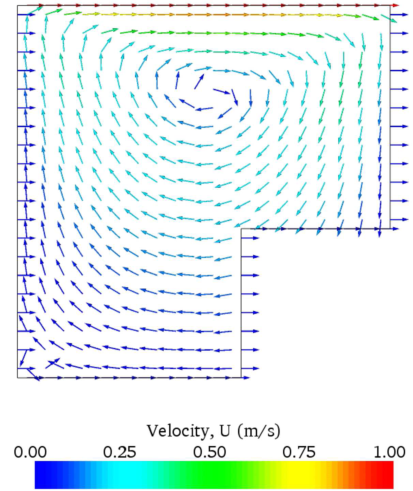
\includegraphics{fig-2-13}
 \caption{\OFcase{cavity}ケースで解いた速度場を
 \OFcase{cavityClipped}上にマッピングした図}
 \label{fig:2.13}
\end{figure}


\begin{figure}[ht]
 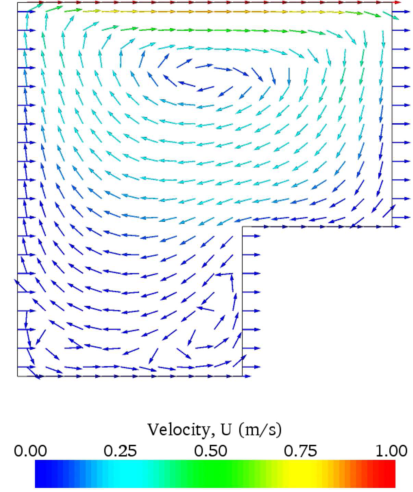
\includegraphics{fig-2-14}
 \caption{速度場の\OFcase{cavityClipped}の解法}
 \label{fig:2.14}
\end{figure}


\OFkeyword{cuttingPatches}リストは,対象パッチを削除した,
元の場の内部の値を写像した対象のパッチを含みます.
本ケースでは,\OFpatch{fixedWalls}を内挿プロセスの実例説明に用いることとします.
\begin{OFverbatim}[file]
cuttingPatches
(
  fixedWalls
);
\end{OFverbatim}
ここで,\OFtool{mapFields}を次のコマンドから実行することができます.
\begin{OFverbatim}[terminal]
mapFields ../cavity
\end{OFverbatim}
\autoref{fig:2.13}に示すような場を確認することができます.
境界パッチは,期待したように元のケースからの値が引き継がれています.
この実例において,\OFpatch{fixedWalls}パッチの速度を$(0, 0, 0)$に
リセットしたい場合があります.このときは,\OFpath{U}をエディタで開き,
\OFpatch{fixedWalls}を\OFkeyword{nonuniform}から
\OFkeyword{uniform (0,0,0)}に変更します.
そして,\OFtool{icoFoam}を実行しましょう.


\subsection{修正した形状の後処理}
\label{ssec:2.1.10}
最初と最後の解析の比較のために,この解析ケースのベクトル図を,
最初の時刻は$0.5\unit{s}$,
次いで$0.6\unit{s}$のように作成することができます.
さらに,幾何形状のアウトラインも示しますが,
これは2次元のケースでは少し注意が必要です.
\PVmenu{Filter}メニューから\PVfilter{Extract Parts}を選択し,
\PVpanel{Parameter}パネルで,興味のあるパッチ,
つまり\OFpatch{lid}と\OFpatch{fixedWalls}をハイライトします.
\PVbutton{Apply}ボタンをクリックし,\PVpanel{Display}パネルで
\PVkeyword{Wireframe}の選択すれば,
ジオメトリのうち選択したものを表示することができます.
\autoref{fig:2.14}は,パッチを黒で表示し,
修正した形状の底部角部分において形成される渦を示しています.



\section{穴あき板の応力解析}
\label{sec:2.2}
\index{あなあきいたのおうりょくかいせき@穴あき板の応力解析}%
\index{チュートリアル!あなあきいたのおうりょくかいせき@穴あき板の応力解析}%
本チュートリアルでは,中央に円形の穴を有する正方形板の
線形弾性定常応力解析における前処理,
実行および後処理の方法を述べます.
板の大きさは,辺長$4\unit{m}$および穴の半径$0.5\unit{m}$です.
さらに\autoref{fig:2.15}に示すように,
板の左右端には$\sigma = 10\unit{kPa}$の一様表面力が負荷されています.
本形状においては二つの対称面が存在するため,
解析領域は\autoref{fig:2.15}のグレーで示した板全体の
4分の1の部分のみをカバーすれば十分です.


\begin{figure}[ht]
 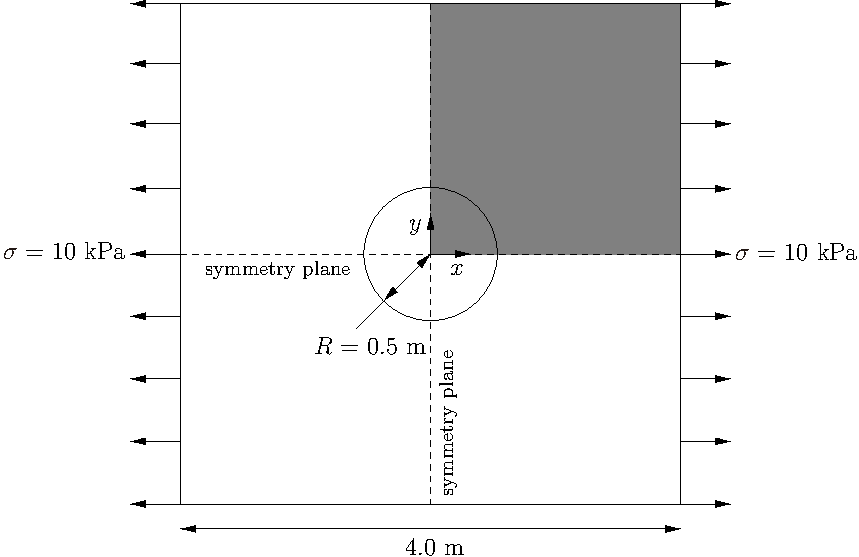
\includegraphics{fig-2-15}
 \caption{穴あき板の形状}
 \label{fig:2.15}
\end{figure}


本問題では,板の面内に応力が負荷されるため,
2次元問題として近似することができます.
Cartesian座標系においては,
この構造の3番目の次元についての振る舞いを考察するにあたって,
以下の二つの仮定をすることができます.
(1) 平面応力条件:2次元平面内以外の方向にはたらく応力成分を無視できるものと仮定します.
(2) 平面ひずみ条件:2次元平面内以外の方向にはたらくひずみ成分を無視できるものと仮定します.
本ケースのように3次元方向に薄い固体に対しては,
平面応力条件が適当です.
なお平面ひずみ条件は,3次元方向に厚い固体に対して適用されます.

円形の穴を有する無限大に大きく薄い板への負荷に対しては,
解析解が存在します.垂直な対称面における法線方向応力の解は以下となります.
\begin{align}
 \label{eq:2.14}
 (\sigma_{xx})_{x=0} =
 \begin{cases}
  \displaystyle
  \sigma\left(1 + \frac{R^{2}}{2y^{2}} + \frac{3R^{4}}{2y^{4}}\right)
  & \text{for}\ |y| \ge R \\
  0 & \text{for}\ |y| < R
 \end{cases}
\end{align}
シミュレーションの実行結果をこの解析解と比較することとしましょう.
チュートリアルの最後に,
メッシュの解像度および非等間隔化に対する解の感度を調べ,
また,穴に対する板の大きさを大きくすることで
無限大板に対する解析解と有限板に対する本問題の解を比較して
誤差を見積もることができるように演習問題を用意しています.


\subsection{メッシュ生成}
\label{ssec:2.2.1}
解析領域は4ブロックからなり,
そのうちのいくつかは円弧形の端部を有します.
$x$--$y$平面におけるメッシュブロックの構造を
\autoref{fig:2.16}に示します.
\autoref{sssec:2.1.1.1}で述べたように,
2次元として扱われるようなケースであっても,
OpenFOAMでは全てのジオメトリが3次元で生成されます.
したがって$z$方向のブロックの大きさを設定しなければなりませんので,
ここでは$0.5\unit{m}$とします.
表面力境界条件は力でなく応力で指定されますので,
断面積すなわち$z$方向の大きさは解に影響を与えません.


\begin{figure}[ht]
 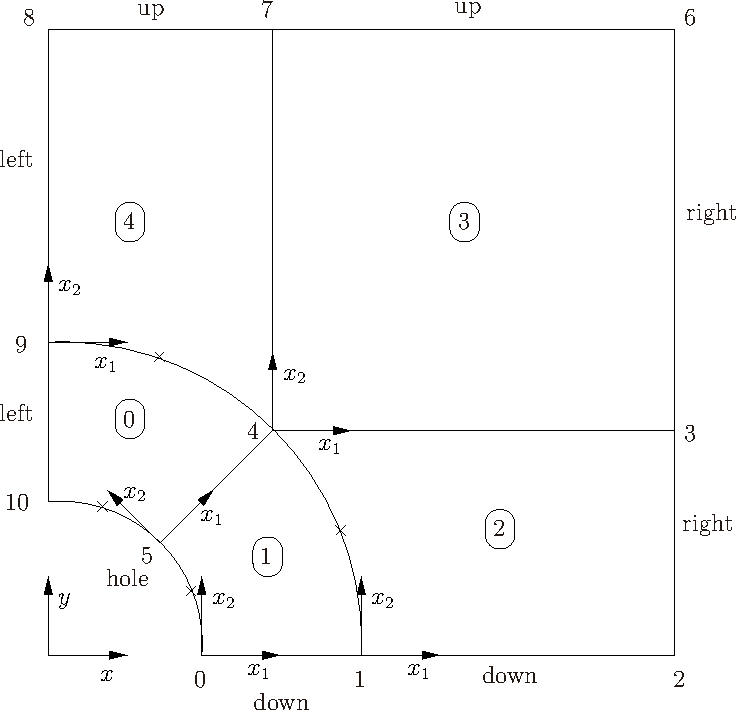
\includegraphics{fig-2-16}
 \caption{穴あき板解析のためのメッシュのブロック構造}
 \label{fig:2.16}
\end{figure}


\OFpath{\$FOAM\_RUN/tutorials/stressAnalysis/solidDisplacementFoam}ディレクトリの
\OFpath{plateHole}ケースに移動し,\OFpath{plateHole}ケースの
\OFpath{constant/polyMesh/blockMeshDict}をエディタで開きます.
\OFdictionary{block\-MeshDict}ディクショナリのエントリを以下に示します.
\begin{OFverbatim}[file, linenum=17]
convertToMeters 1;

vertices
(
    (0.5 0 0)
    (1 0 0)
    (2 0 0)
    (2 0.707107 0)
    (0.707107 0.707107 0)
    (0.353553 0.353553 0)
    (2 2 0)
    (0.707107 2 0)
    (0 2 0)
    (0 1 0)
    (0 0.5 0)
    (0.5 0 0.5)
    (1 0 0.5)
    (2 0 0.5)
    (2 0.707107 0.5)
    (0.707107 0.707107 0.5)
    (0.353553 0.353553 0.5)
    (2 2 0.5)
    (0.707107 2 0.5)
    (0 2 0.5)
    (0 1 0.5)
    (0 0.5 0.5)
);

blocks
(
    hex (5 4 9 10 16 15 20 21) (10 10 1) simpleGrading (1 1 1)
    hex (0 1 4 5 11 12 15 16) (10 10 1) simpleGrading (1 1 1)
    hex (1 2 3 4 12 13 14 15) (20 10 1) simpleGrading (1 1 1)
    hex (4 3 6 7 15 14 17 18) (20 20 1) simpleGrading (1 1 1)
    hex (9 4 7 8 20 15 18 19) (10 20 1) simpleGrading (1 1 1)
);

edges
(
    arc 0 5 (0.469846 0.17101 0)
    arc 5 10 (0.17101 0.469846 0)
    arc 1 4 (0.939693 0.34202 0)
    arc 4 9 (0.34202 0.939693 0)
    arc 11 16 (0.469846 0.17101 0.5)
    arc 16 21 (0.17101 0.469846 0.5)
    arc 12 15 (0.939693 0.34202 0.5)
    arc 15 20 (0.34202 0.939693 0.5)
);

boundary
(
    left
    {
        type symmetryPlane;
        faces
        (
            (8 9 20 19)
            (9 10 21 20)
        );
    }
    right
    {
        type patch;
        faces
        (
            (2 3 14 13)
            (3 6 17 14)
        );
    }
    down
    {
        type symmetryPlane;
        faces
        (
            (0 1 12 11)
            (1 2 13 12)
        );
    }
    up
    {
        type patch;
        faces
        (
            (7 8 19 18)
            (6 7 18 17)
        );
    }
    hole
    {
        type patch;
        faces
        (
            (10 5 16 21)
            (5 0 11 16)
        );
    }
    frontAndBack
    {
        type empty;
        faces
        (
            (10 9 4 5)
            (5 4 1 0)
            (1 4 3 2)
            (4 7 6 3)
            (4 9 8 7)
            (21 16 15 20)
            (16 11 12 15)
            (12 13 14 15)
            (15 14 17 18)
            (15 18 19 20)
        );
    }
);

mergePatchPairs
(
);

// ************************************************************************* //
\end{OFverbatim}
ここまで前のチュートリアルのように
直線的なエッジの形状を対象としてきましたが,
本チュートリアルでは曲線のエッジについて定義する必要があります.
\OFkeyword{edges}のキーワードエントリ(曲線エッジのリスト)内で
曲線エッジが定義されています.
それらのリストの構文では,最初に\OFkeyword{arc},
\OFkeyword{simpleSpline},\OFkeyword{polyLine}などの
曲線タイプが示されていますが,
さらに詳しくは\autoref{ssec:5.3.1}を参照してください.
この例題ではすべてのエッジが円弧なので\OFkeyword{arc}を使用します.
曲線を\OFkeyword{arc}で定義する際は始点と終点および
円弧上の点の3点によって指定します.

この
\index{blockMeshDict@\OFdictionary{blockMeshDict}!ディクショナリ}%
\index{ディクショナリ!blockMeshDict@\OFdictionary{blockMeshDict}}%
\OFdictionary{blockMeshDict}に含まれるブロック全てが
同じ方向を向いているわけではありません.
\autoref{fig:2.16}に示すように,
ブロック0の$x_{2}$方向はブロック4の$-x_{1}$方向と同じになっています.
このためブロック界面でセルが矛盾なく合うよう,
それぞれのブロックにおけるセルの番号および順序を
決定する際には注意を払わねばなりません.

プレートの全側面,穴の面,前後面の六つのパッチが定義されます.
そのうち左の面 (\OFpatch{left}) と下の面 (\OFpatch{down}) は対称面です.
このようなことはジオメトリ上の制限であるため,
ただの場の境界条件とするよりはメッシュの定義の中に組み込んで作ります.
よって,このパッチは\OFdictionary{blockMeshDict}内の
特別な\OFkeyword{SymmetryPlane}タイプを
使って定義するとよいでしょう.
\OFpatch{frontAndBack}パッチは2次元問題の場合は
無視される面を示しています.
これは先ほども言ったようにジオメトリ上の制限なので,
\OFdictionary{blockMeshDict}内の\OFkeyword{empty}タイプを使って定義しましょう.
境界条件に関してさらに詳しくは\autoref{ssec:5.2.1}を参照してください.
そのほかのパッチは通常の\OFkeyword{patch}タイプです.
メッシュは\OFtool{blockMesh}を使って生成し,
\autoref{ssec:2.1.2}に述べたようにして\OFtool{paraFoam}で見ることができます.
メッシュは\autoref{fig:2.17}のようになります.


\begin{figure}[ht]
 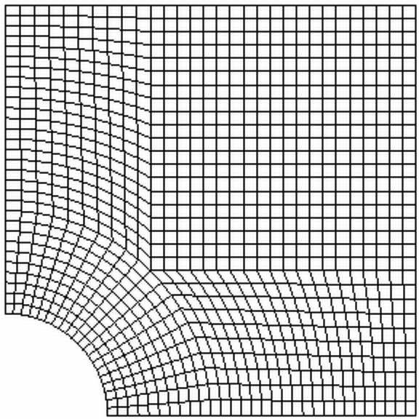
\includegraphics{fig-2-17}
 \caption{穴あき板問題のための解析メッシュ}
 \label{fig:2.17}
\end{figure}


\subsubsection{境界および初期条件}
\label{sssec:2.2.1.1}
メッシュの生成ができたら初期条件と境界条件を設定します.
熱抵抗を考慮しない応力解析では,
変位\OFkeyword{D}のみ設定する必要があります.
\OFpath{0/D}のファイルは以下のようになります.
\begin{OFverbatim}[file, linenum=17]
dimensions      [0 1 0 0 0 0 0];

internalField   uniform (0 0 0);

boundaryField
{
    left
    {
        type            symmetryPlane;
    }
    right
    {
        type            tractionDisplacement;
        traction        uniform ( 10000 0 0 );
        pressure        uniform 0;
        value           uniform (0 0 0);
    }
    down
    {
        type            symmetryPlane;
    }
    up
    {
        type            tractionDisplacement;
        traction        uniform ( 0 0 0 );
        pressure        uniform 0;
        value           uniform (0 0 0);
    }
    hole
    {
        type            tractionDisplacement;
        traction        uniform ( 0 0 0 );
        pressure        uniform 0;
        value           uniform (0 0 0);
    }
    frontAndBack
    {
        type            empty;
    }
}

// ************************************************************************* //
\end{OFverbatim}
まず,変位の初期条件が$(0, 0, 0)\unit{m}$になっています.
\OFpath{Constant/polyMesh/boundaries}のメッシュの記述にあるように,
\OFpatch{left}と\OFpatch{down}のパッチは
\OFkeyword{type}が\OFkeyword{symmetryPlane}である必要があります.
同様に\OFpatch{frontAndBack}は\OFkeyword{empty}になります.

その他のパッチは表面力境界条件です.表面力境界条件は,
(1) キーワード
\index{traction@\OFkeyword{traction}!キーワード}%
\index{キーワード!traction@\OFkeyword{traction}}%
\OFkeyword{traction}で表される,境界面における表面力ベクトル,
(2) キーワード
\index{pressure@\OFkeyword{pressure}!キーワード}%
\index{キーワード!pressure@\OFkeyword{pressure}}%
\OFkeyword{pressure}で表される,
境界面の法線方向に働く表面力となる(外向きの場合は負値となる)圧力,
の線形結合で指定されます.
\OFpatch{up}および\OFpatch{hole}パッチは表面力ゼロであるため,
表面力ベクトルおよび圧力ともにゼロが設定されます.
\OFpatch{right}パッチについては,\autoref{fig:2.24}に示すように,
表面力ベクトルは$(1\mathrm{e}4, 0, 0)\unit{Pa}$,
圧力は$0\unit{Pa}$が設定されます.
変位の初期条件は全て$(0, 0, 0)\unit{m}$が設定されます.

\subsubsection{機械的性質}
\label{sssec:2.2.1.2}
本ケースにおける物性値は
\index{mechanicalProperties@\OFdictionary{mechanicalProperties}!ディクショナリ}%
\index{ディクショナリ!mechanicalProperties@\OFdictionary{mechanicalProperties}}%
\OFdictionary{mechanicalProperties}ディクショナリによって設定します.
本問題においては,\autoref{tbl:2.1}に示す
鋼の機械的性質を指定する必要があります.
さらに本ディクショナリで\OFkeyword{planeStress}を\OFkeyword{yes}に設定しなければなりません.


\begin{table}[ht]
 %#! platex UserGuideJa
\begin{tabular}{lccc}
 物性 & 単位 & キーワード & 値 \\
 \hline
 密度 & $\unit*{kg\,m^{-3}}$ & \OFkeyword{rho} & 7854 \\
 ヤング率 & $\unit*{Pa}$ & \OFkeyword{E} & $2 \times 10^{11}$ \\
 ポアソン比 & --- & \OFkeyword{nu} & 0.3 \\
 \hline
\end{tabular}

 \caption{鋼の機械的性質}
 \label{tbl:2.1}
\end{table}


\subsubsection{熱的性質}
\label{sssec:2.2.1.3}
運動によって発生する熱応力によって
運動方程式と連成した熱方程式を解くことができるよう,
\index{solidDisplacementFoam@\OFtool{solidDisplacementFoam}!ソルバ}%
\index{ソルバ!solidDisplacementFoam@\OFtool{solidDisplacementFoam}}%
\OFtool{solidDisplacementFoam}ソルバには温度場を表す変数\OFkeyword{T}が存在します.
\index{thermalProperties@\OFdictionary{thermalProperties}!ディクショナリ}%
\index{ディクショナリ!thermalProperties@\OFdictionary{thermalProperties}}%
\OFdictionary{thermalProperties}ディクショナリの\OFkeyword{thermalStress}スイッチによって,
OpenFOAMが熱方程式を解くべきかどうかを実行時に指定します.
また本ディクショナリによって,
本ケースすなわち\autoref{tbl:2.2}に示す
鋼の熱的性質を指定します.


\begin{table}[ht]
 %#! platex ProgrammersGuideJa
\begin{tabular}{|cccc|}
 \hline
 \tblstrut
 項の記述 & 陰的・陽的 & 記述 & \OFclass{fvm::}または\OFclass{fvc::}の関数 \\
 \hline\hline
 \tblstrut
 ラプラシアン & 陰的・陽的 & $\nabla^{2}\phi$ & \texttt{laplacian(phi)} \\
 &  & $\nabla \inProd \varGamma \nabla \phi$ & \texttt{laplacian(Gamma, phi)} \\
 \hline
 \tblstrut
 時間微分 & 陰的・陽的 & $\frac{\partial\phi}{\partial t}$ & \texttt{ddt(phi)} \\
 &  & $\frac{\partial\rho\phi}{\partial t}$ & \texttt{ddt(rho, phi)} \\
 \hline
 \tblstrut
 時間の2階微分 & 陰的・陽的 & $\frac{\partial}{\partial t}\left(\rho\frac{\partial\phi}{\partial t}\right)$ & \texttt{d2dt2(rho, phi)} \\
 \hline
 \tblstrut
 移流 & 陰的・陽的 & $\nabla \inProd (\psi)$ & \verb|div(psi, scheme)*| \\
 &  & $\nabla \inProd (\psi\phi)$ & \verb|div(psi, phi, word)*| \\
 &  &  & \verb|div(psi, phi)| \\
 \hline
 \tblstrut
 発散 & 陽的 & $\nabla \inProd \chi$ & \texttt{div(chi)} \\
 \hline
 \tblstrut
 勾配 & 陽的 & $\nabla \chi$ & \texttt{grad(chi)} \\
 &  & $\nabla \phi$ & \texttt{gGrad(phi)} \\
 &  &  & \texttt{lsGrad(phi)} \\
 &  &  & \texttt{snGrad(phi)} \\
 &  &  & \texttt{snGradCorrection(phi)} \\
 \hline
 \tblstrut
 勾配の勾配の二乗 & 陽的 & $|\nabla\nabla\phi|^{2}$ & \texttt{sqrGradGrad(phi)} \\
 \hline
 \tblstrut
 回転 & 陽的 & $\nabla \times \phi$ & \texttt{curl(phi)} \\
 \hline
 \tblstrut
 湧き出し & 陰的 & $\rho\phi$ & \texttt{Sp(rho, phi)} \\
 & 陰的・陽的\textsuperscript{\dag} &  & \texttt{SuSp(rho, phi)} \\
 \hline
 \multicolumn{4}{l}{\tblstrut\dag\ 湧き出し\OFkeyword{fvm::SuSp}は
 \OFkeyword{rho}の符号に依存して,陰的または陽的に離散化されます.} \\
 \multicolumn{4}{l}{\dag\ 陽的な湧き出しは単純に
 \OFclass{vol<Type>Field}で指定されます.例:\texttt{rho*phi}} \\
 \multicolumn{4}{l}{関数の引数は以下のようなクラスです.} \\
 \multicolumn{4}{l}{\OFkeyword{phi}: \OFclass{vol<Type>Field}} \\
 \multicolumn{4}{l}{\OFkeyword{Gamma}: \OFclass{scalar},\OFclass{volScalarField},
 \OFclass{volTensorField},\OFclass{surfaceTensorField}.} \\
 \multicolumn{4}{l}{\OFkeyword{rho}: \OFclass{scalar},\OFclass{volScalarField}} \\
 \multicolumn{4}{l}{\OFkeyword{psi}: \OFclass{surfaceTensorField}} \\
 \multicolumn{4}{l}{\OFkeyword{chi}: \OFclass{surface<Type>Field},\OFclass{vol<Type>Field}} \\
\end{tabular}

 \caption{鋼の熱的性質}
 \label{tbl:2.2}
\end{table}


本ケースにおいては熱の方程式は解きません.
したがって\OFdictionary{thermalProperties}ディクショナリにおける
\OFkeyword{thermalStress}キーワードエントリは\OFkeyword{no}に設定します.

\subsubsection{制御}
\label{sssec:2.2.1.4}
通常どおり,解法の制御に関する情報は\OFdictionary{controlDict}ディクショナリから
読み込まれます.本ケースでは,\OFkeyword{startTime}は0です.
本ケースは定常状態ですので,時間刻みは重要ではありません.
このような状況では,
定常状態のケースにおける反復回数カウンタとして働くよう,
時間刻み\OFkeyword{deltaT}を1に設定するのが最善です.
このようにした場合,本ケースで100に設定した\OFkeyword{endTime}は
反復回数の上限として働きます.\OFkeyword{writeInterval}は20に設定します.

\index{controlDict@\OFdictionary{controlDict}!ディクショナリ}%
\index{ディクショナリ!controlDict@\OFdictionary{controlDict}}%
\OFdictionary{controlDict}のエントリは以下のようになります.
\begin{OFverbatim}[file, linenum=17]

application     solidDisplacementFoam;

startFrom       startTime;

startTime       0;

stopAt          endTime;

endTime         100;

deltaT          1;

writeControl    timeStep;

writeInterval   20;

purgeWrite      0;

writeFormat     ascii;

writePrecision  6;

writeCompression off;

timeFormat      general;

timePrecision   6;

graphFormat     raw;

runTimeModifiable true;


// ************************************************************************* //
\end{OFverbatim}

\subsubsection{離散化スキームおよび線形方程式ソルバ制御}
\label{sssec:2.2.1.5}
次は\OFdictionary{fvSchemes}ディクショナリについて見てみましょう.
まず,この問題は定常状態ですので,
\OFkeyword{timeScheme}における時間微分としては\OFkeyword{steadyState}を選択します.
これによって時間微分項がオフの状態になります.
全てのソルバが定常状態および過渡的状態の双方に対して
適用可能な訳ではありませんが,
\OFtool{solidDisplacementFoam}は基本的なアルゴリズムが
双方のシミュレーションともに共通であるため,
双方に適用可能となっています.

線形弾性応力解析における運動方程式には,
変位の勾配を含む陽な項がいくつか存在します.
この勾配を正確かつ滑らかに評価できれば,良い計算結果が得られます.
通常,有限体積法における離散化は,
\index{こうばい@勾配!Gaussのていり@Gaussの定理}%
Gaussの定理に基づいています.
Gauss法は大抵の目的においては十分に正確ですが,
本ケースにおいては
\index{こうばい@勾配!さいしょうにじょうフィット@最小二乗フィット}%
\index{こうばい@勾配!さいしょうにじょうほう@最小二乗法}%
最小二乗法を使用することとします.
したがって
\index{fvSchemes@\OFdictionary{fvSchemes}!ディクショナリ}%
\index{ディクショナリ!fvSchemes@\OFdictionary{fvSchemes}}%
\OFdictionary{fvSchemes}ディクショナリを開き,
\OFkeyword{grad(U)}勾配離散化スキームとして
\index{leastSquares@\OFkeyword{leastSquares}!キーワード}%
\index{キーワード!leastSquares@\OFkeyword{leastSquares}}%
\OFkeyword{leastSquares}を選択してください.
\begin{OFverbatim}[file, linenum=17]

d2dt2Schemes
{
    default         steadyState;
}

ddtSchemes
{
    default         Euler;
}

gradSchemes
{
    default         leastSquares;
    grad(D)         leastSquares;
    grad(T)         leastSquares;
}

divSchemes
{
    default         none;
    div(sigmaD)     Gauss linear;
}

laplacianSchemes
{
    default         none;
    laplacian(DD,D) Gauss linear corrected;
    laplacian(DT,T) Gauss linear corrected;
}

interpolationSchemes
{
    default         linear;
}

snGradSchemes
{
    default         none;
}

fluxRequired
{
    default         no;
    D               yes;
    T               no;
}


// ************************************************************************* //
\end{OFverbatim}
\OFpath{system}ディレクトリにある
\OFdictionary{fvSolution}ディクショナリでは,
求解に使用される線形方程式のソルバおよびアルゴリズムを設定します.
まず\OFsubdictionary{solvers}サブディクショナリを見ると,
\OFkeyword{D}の
\index{solver@\OFkeyword{solver}!キーワード}%
\index{キーワード!solver@\OFkeyword{solver}}%
\OFkeyword{solver}が
\index{GAMG@\OFkeyword{GAMG}!キーワードエントリ}%
\index{キーワードエントリ!GAMG@\OFkeyword{GAMG}}%
\OFkeyword{GAMG}になっていることがわかります.
\index{tolerance@\OFkeyword{tolerance}!キーワード}%
\index{キーワード!tolerance@\OFkeyword{tolerance}}%
\OFkeyword{tolerance}で表される
ソルバ許容値(ソルバ名の次の数値)は,本問題では$10^{-6}$を設定します.
\index{relTol@\OFkeyword{relTol}!キーワード}%
\index{キーワード!relTol@\OFkeyword{relTol}}%
\OFkeyword{relTol}で表される
ソルバの相対許容値(さらにその次の数値)には
各反復ごとの残差の所要低減量を設定します.
本問題においては多くの項が陽であり,
また個別の反復的手順の一部としてアップデートされるため,
各反復において厳しい相対許容値を設定することは非効率的です.
したがって相対許容値として合理的な値は$0.01$,
もしくはさらに高めの$0.1$,
あるいはせいぜいこのケースのように$0.9$程度にしておきます.
\begin{OFverbatim}[file, linenum=17]

solvers
{
    "(D|T)"
    {
        solver          GAMG;
        tolerance       1e-06;
        relTol          0.9;
        smoother        GaussSeidel;
        cacheAgglomeration true;
        nCellsInCoarsestLevel 20;
        agglomerator    faceAreaPair;
        mergeLevels     1;
    }
}

stressAnalysis
{
    compactNormalStress yes;
    nCorrectors     1;
    D               1e-06;
}


// ************************************************************************* //
\end{OFverbatim}
\OFdictionary{fvSolution}ディクショナリは,
アプリケーションソルバに特有の制御パラメータを含む
\OFsubdictionary{stressAnalysis}サブディクショナリを含みます.
まず,各時刻ステップ内での表面力境界条件処理を含めた,
全方程式系に関する外側ループの数を指定する\OFkeyword{nCorrectors}があります.
本問題は定常状態を扱いますので,
「時刻ステップ」を反復回数カウンタとして使い収束解へと向かう
反復を実行することになります.
したがって\OFkeyword{nCorrectors}を1に設定します.

\OFkeyword{D}キーワードには外側反復ループにおける収束許容値,
すなわち初期残差に対して反復計算によって消去されるべき
レベルを設定します.
本問題では前述において設定したソルバ許容値の$10^{-6}$に設定します.


\subsection{コードの実行}
\label{ssec:2.2.2}
以下に示すようなコマンドによって,
実行後にログファイルに記録された収束状況を見ることができるよう,
バックグラウンドでコードを実行します.
\begin{OFverbatim}[terminal]
cd $FOAM_RUN/tutorials/stressAnalysis/solidDisplacementFoam/plateHole
solidDisplacementFoam > log &
\end{OFverbatim}%$
実行後には生成されたログファイルを見て,
反復回数および解を求める各方向変位の初期・最終残差などの
収束状況を確認できます.
本ケースの反復許容回数設定では,
最終残差は必ず初期残差の$0.1$倍以下となるはずです.
いったん両初期残差ともに$10^{-6}$の収束許容残差以下となれば,
その計算は収束したとみなしバッチジョブを\texttt{kill}することによって
止めることができます.


\subsection{後処理}
\label{ssec:2.2.3}
後処理は\autoref{ssec:2.1.4}と
同様に行うことができます.
\OFtool{solidDisplacementFoam}ソルバは,
応力場$\sigma$を対称テンソル場として出力します.
したがって例えば,$\sigma_{xx}$を\OFtool{paraFoam}で見ることができます.
OpenFOAMソルバにおける変数名は通常,
それらを表す数学記号にならって名付けられることは,
ここで再度述べるに値するでしょう.ギリシア記号の場合は,
変数は発音どおりに名付けられます.例えば,
$\sigma_{xx}$は\OFkeyword{sigmaxx}と名付けられます.

独立したスカラ成分の$\sigma_{xx}$や$\sigma_{xy}$などは,
\autoref{sssec:2.1.5.7}で述べた\OFtool{foamCalc}を\OFkeyword{sigma}に関して実行して求めます.
\begin{OFverbatim}[terminal]
foamCalc components sigma
\end{OFverbatim}
\OFkeyword{sigmaxx}や\OFkeyword{sigmaxy}などと名づけられた成分の
ファイルが時間のディレクトリに生成されます.
\autoref{fig:2.18}のように応力を\OFtool{paraFoam}で見ることができます.


\begin{figure}[ht]
 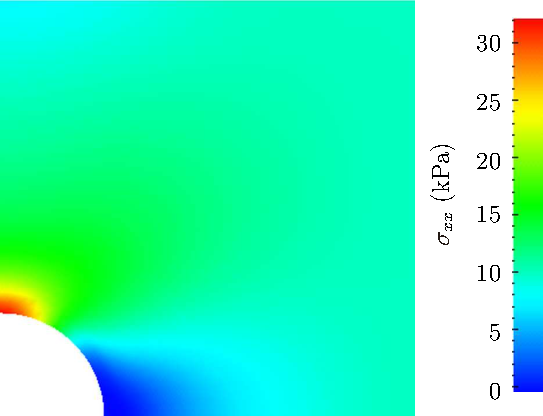
\includegraphics{fig-2-18}
 \caption{穴あき板における応力場}
 \label{fig:2.18}
\end{figure}


\autoref{eq:2.14} の解析解と
ここで得られた数値解を比較しましょう.
そのためには,解析領域左端の対称面に沿ってのデータを
出力しなければなりません.
このようなグラフのために必要なデータは,
\OFtool{sample}ユーティリティによって作成することができます.
\OFtool{sample}の設定は\OFpath{system}ディレクトリ内の\OFpath{sampleDict}で行い
詳細は\autoref{tbl:6.3}に要約しています.
データのサンプリングを行う座標区間は,
\OFkeyword{sets}によって$(0.0, 0.5, 0.25)$から$(0.0, 2.0, 0.25)$に指定されています.
物理量は\OFkeyword{fields}に指定します.
\begin{OFverbatim}[file, linenum=17]

interpolationScheme cellPoint;

setFormat       raw;

sets
(
    leftPatch
    {
        type    uniform;
        axis    y;
        start   ( 0 0.5 0.25 );
        end     ( 0 2 0.25 );
        nPoints 100;
    }
);

fields          ( sigmaxx );


// ************************************************************************* //
\end{OFverbatim}
通常通り\OFtool{sample}を実行してください.
\index{writeFormat@\OFkeyword{writeFormat}!キーワード}%
\index{キーワード!writeFormat@\OFkeyword{writeFormat}}%
\OFkeyword{writeFormat}は\OFkeyword{raw}形式で2列のフォーマットとなっています.
データは\OFpath{postProcessing/sets}ディレクトリの時刻サブディレクトリの中のファイルに書き込まれます.
たとえば,時刻$t = 100\unit{s}$のデータは
\OFpath{postProcessing/sets/100/leftPatch\_sigmaxx.xy}に書き込まれます.
GnuPlotのようなアプリケーションでは,
コマンドプロンプトで以下を入力することで,
数値解および解析解の両方をプロットすることができます.
\begin{OFverbatim}[terminal]
plot [0.5:2] [0:] 'postProcessing/sets/100/leftPatch_sigmaxx.xy',
     1e4*(1+(0.125/(x**2))+(0.09375/(x**4)))
\end{OFverbatim}
プロット例を\autoref{fig:2.19}に示します.


\begin{figure}[ht]
 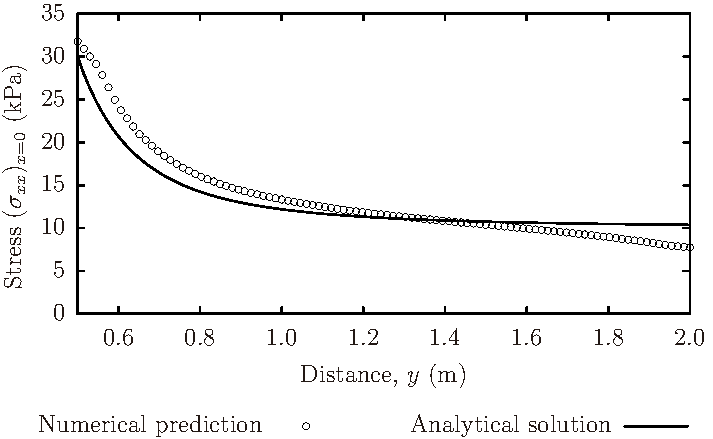
\includegraphics{fig-2-19}
 \caption{垂直方向対称面における法線方向応力}
 \label{fig:2.19}
\end{figure}


\subsection{演習}
\label{ssec:2.2.4}
以下は\OFtool{solidDisplacementFoam}に習熟していただくための演習課題です.

\subsubsection{メッシュ解像度の増加}
\label{sssec:2.2.4.1}
$x$,$y$方向それぞれのメッシュ解像度を増やしてみましょう.
\autoref{ssec:2.2.3}の最終的な粗メッシュの結果を,
\index{mapFields@\OFtool{mapFields}!ユーティリティ}%
\index{ユーティリティ!mapFields@\OFtool{mapFields}}%
\OFtool{mapFields}を使って密メッシュの初期条件にマッピングしてください.

\subsubsection{非等間隔メッシュの導入}
\label{sssec:2.2.4.2}
穴に近いセルが遠いセルより密になるよう,
メッシュ幅を変化させてください.
隣接するセルの大きさの比率が$1.1$以上にならないように,
またブロック間のセルの大きさの比率がブロック内の比率と
同様となるようメッシュを作成してください.
メッシュの非等間隔化については\autoref{ssec:2.1.6}で述べました.
ここでも,\autoref{ssec:2.2.3}の最終的な粗メッシュでの結果を,
\OFtool{mapFields}を使って非等間隔メッシュの初期条件としてマッピングします.
結果を解析解および非等間隔化する前の結果と比較してみましょう.
等間隔メッシュと同一のセル数を使用した場合,
解の精度は改善されるでしょうか?

\subsubsection{板の大きさの変更}
\label{sssec:2.2.4.3}
ここで示されている解析解は,
有限な大きさの穴を有する無限大板におけるものです.
したがって有限な大きさの板においては,
この解析解は必ずしも正確ではありません.
誤差を見積もるために,
穴の大きさを同一に保ったまま板を大きくしてみましょう.



\section{ダムの決壊}
\label{sec:2.3}
\index{ダムのけっかい@ダムの決壊}%
\index{チュートリアル!ダムのけっかい@ダムの決壊}%
このチュートリアルでは,\OFtool{interFoam}を用いて,
単純化したダム決壊の2次元問題を解くことにします.
この問題の特徴は,くっきりとした界面や
\index{じゆうひょうめん@自由表面}%
自由表面によって
隔てられている二つの流体による非定常の流れ場であることです.
\OFtool{interFoam}における2相流体を解くアルゴリズムは,
Volume of fluid (VOF) 法によるものであり,
ここでは特別な輸送方程式を解いて,
計算格子における2相の体積分率,
もしくは相比率$\alpha$を決定します.
各物理量は,この相比率に(各流体の)密度をかけた
平均的な値として算出されます.
個々の物質の界面は,VOF法ではその性質上明示的には解かれず,
相比率場の特性として浮き上がってくるということになります.
相比率は0から1の間の任意の値をとり得るため,
界面は決してくっきりと定義されませんので,
本来のくっきりとした界面が存在するべき領域の周辺を,
(計算上の)界面がぼんやりと占めることになります.

計算条件では,貯水池の左側に,膜で仕切られた水柱が最初存在します.
時刻$t = 0\unit{s}$に,膜が取り除かれて,水柱が崩れだします.
崩壊しながら,水流は貯水槽の底にある出っ張りにぶつかり,
いくつかの気泡を含む,複雑な流れ場の様相を呈します.
計算形状と初期条件は\autoref{fig:2.20}に示しました.


\begin{figure}[ht]
 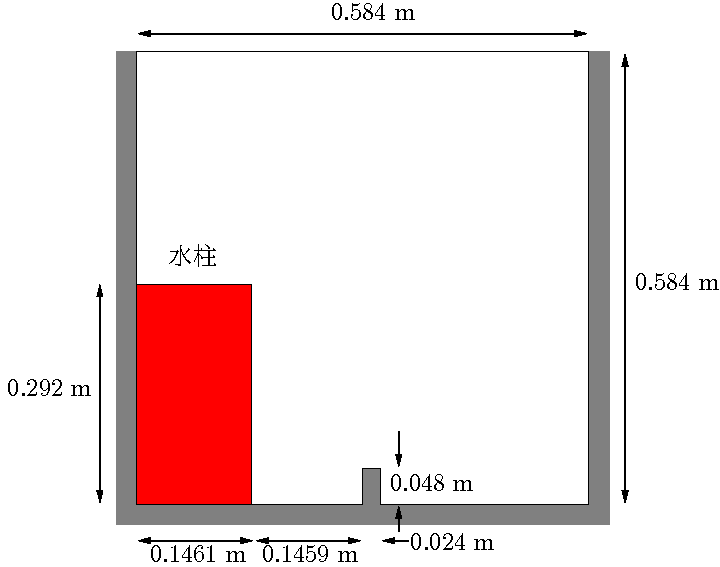
\includegraphics{fig-2-20}
 \caption{ダム決壊の計算形状}
 \label{fig:2.20}
\end{figure}


\subsection{格子の生成}
\label{ssec:2.3.1}
\OFpath{\$FOAM\_RUN/tutorials/multiphase/interFoam/laminar}にある
\OFpath{damBreak}のケースディレクトリに移動しましょう.
前述した方法で\OFtool{blockMesh}を実行して格子を生成してください.
この\OFcase{damBreak}のメッシュは五つのブロックで構成されます.
\OFdictionary{blockMeshDict}の中身を以下に示します.
\begin{OFverbatim}[file, linenum=17]

convertToMeters 0.146;

vertices        
(
    (0 0 0)
    (2 0 0)
    (2.16438 0 0)
    (4 0 0)
    (0 0.32876 0)
    (2 0.32876 0)
    (2.16438 0.32876 0)
    (4 0.32876 0)
    (0 4 0)
    (2 4 0)
    (2.16438 4 0)
    (4 4 0)
    (0 0 0.1)
    (2 0 0.1)
    (2.16438 0 0.1)
    (4 0 0.1)
    (0 0.32876 0.1)
    (2 0.32876 0.1)
    (2.16438 0.32876 0.1)
    (4 0.32876 0.1)
    (0 4 0.1)
    (2 4 0.1)
    (2.16438 4 0.1)
    (4 4 0.1)
);

blocks          
(
    hex (0 1 5 4 12 13 17 16) (23 8 1) simpleGrading (1 1 1)
    hex (2 3 7 6 14 15 19 18) (19 8 1) simpleGrading (1 1 1)
    hex (4 5 9 8 16 17 21 20) (23 42 1) simpleGrading (1 1 1)
    hex (5 6 10 9 17 18 22 21) (4 42 1) simpleGrading (1 1 1)
    hex (6 7 11 10 18 19 23 22) (19 42 1) simpleGrading (1 1 1)
);

edges           
(
);

boundary
(
    leftWall
    {
        type wall;
        faces
        (
            (0 12 16 4)
            (4 16 20 8)
        );
    }
    rightWall
    {
        type wall;
        faces
        (
            (7 19 15 3)
            (11 23 19 7)
        );
    }
    lowerWall
    {
        type wall;
        faces
        (
            (0 1 13 12)
            (1 5 17 13)
            (5 6 18 17)
            (2 14 18 6)
            (2 3 15 14)
        );
    }
    atmosphere
    {
        type patch;
        faces
        (
            (8 20 21 9)
            (9 21 22 10)
            (10 22 23 11)
        );
    }
);

mergePatchPairs
(
);

// ************************************************************************* //
\end{OFverbatim}


\subsection{境界条件}
\label{ssec:2.3.2}
\OFpath{constant/polyMesh}ディレクトリの\OFpath{boundary}ファイルを見ることで
\OFtool{blockMesh}で生成された境界の形状を確認しましょう.
\OFpatch{leftWall},\OFpatch{rightWall},\OFpatch{lowerWall},
\OFpatch{atmosphere},\OFpatch{defaultFaces}の
五つの境界パッチがあります.
パッチの種類について理解しておきましょう.
\OFpatch{atmosphere}は何の属性もなく,
単に境界条件によって規定される標準の\OFboundary{patch}です.
\OFpatch{defaultFaces}は,本ケースでは2次元であるため
パッチの法線方向を解析の対象としないため,\OFboundary{empty}とします.
\OFpatch{leftWall},\OFpatch{rightWall},
\OFpatch{lowerWall}はそれぞれ
\index{wall@\OFboundary{wall}!きょうかいじょうけん@境界条件}%
\index{きょうかいじょうけん@境界条件!wall@\OFboundary{wall}}%
\OFboundary{wall}です.
ただの\OFboundary{patch}と同様に\OFboundary{wall}もメッシュについて形状や位相の情報をもちませんが,
壁として識別することができるので,
アプリケーションに特殊な壁表面のモデリングを明示するために
\OFboundary{wall}と定義しています.

\OFtool{interFoam}のソルバが,界面と壁面との接点における
表面張力に対するモデルを含んでいる,というのがよい例です.
このモデルは\OFkeyword{alpha} ($\alpha$) 場の
\index{alphaContactAngle@\OFboundary{alphaContactAngle}!きょうかいじょうけん@境界条件}%
\index{きょうかいじょうけん@境界条件!alphaContactAngle@\OFboundary{alphaContactAngle}}%
\OFboundary{alphaContactAngle}の境界条件と関連付けられています.
その場合,静的な接触角度\OFkeyword{theta0} $\theta_{0}$や,
前縁や後縁における動的な接触角度である
\OFkeyword{thetaA} $\theta_{\mathrm{A}}$と\OFkeyword{thetaR} $\theta_{\mathrm{R}}$,
そして,動的な接触角度において速度に比例する係数
\OFkeyword{uTheta}を指定する必要があります.

このチュートリアルでは,壁面と界面間の表面張力による効果を
無視することにしたいと思います.
それは,静的な接触角度を$\theta_{0} = 90\degree$に,
速度比例係数を$0$と設定することで可能です.
しかしながら,壁の境界条件として,
通常の\OFkeyword{wall}タイプの境界条件を指定する別なやり方もあります.
この場合,\OFkeyword{alpha}に対して\OFkeyword{alphaContactAngle}の境界条件を設定する代わりに,
\OFkeyword{zeroGradient}に設定します.

\OFpatch{top}の境界は大気に対して開放されていることから,
内部流れに応じて流出・流入のいずれも可能にしておく必要があります.
したがって,以下のような,安定性を維持しながらこれを可能にするような
圧力と速度に対する境界条件の組み合わせを用いることになります.
\begin{itemize}
 \item \OFboundary{totalPressure}は,与えられた全圧\OFkeyword{p0}と
       局所速度\OFkeyword{U}から計算される\OFboundary{fixedValue}条件です.
 \item \OFboundary{pressureInletOutletVelocity}は
       全成分に\OFboundary{zeroGradient}を適用しますが,
       流入がある場合は例外として\OFboundary{fixedValue}が
\OFrevision{法線成分では?}%
       \OFemph{接線}成分に適用されます
 \item \OFboundary{inletOutlet}は,流れが外向きならば\OFboundary{zeroGradient}であり,
       流れが内向きならば\OFboundary{fixedValue}です
\end{itemize}
すべての壁の境界においては,圧力場には\OFboundary{fixedFluxPressure}境界条件を適用しますが,
これは境界のフラックスが速度の境界条件にマッチするように圧力勾配を調整するものです.

2次元問題における前後の面を表している\OFpatch{defaultFaces}パッチは,
通常通り\OFkeyword{empty}タイプにします.


\subsection{初期条件の設定}
\label{ssec:2.3.3}
これまでのケースと異なり,ここでは相比率$\alpha_{\mathrm{water}}$に対して,
以下のような非一様な初期条件を与えます.
\begin{align}
 \label{eq:2.15}
 \alpha_{\mathrm{water}} =
 \begin{cases}
  1 & \text{水の相について} \\
  0 & \text{空気の相について}
 \end{cases}
\end{align}
これは,
\index{setFields@\OFtool{setFields}!ユーティリティ}%
\index{ユーティリティ!setFields@\OFtool{setFields}}%
\OFtool{setFields}ユーティリティを実行することによって行います.
この実行には\OFpath{system}ディレクトリ内の\OFpath{setFieldsDict}を必要とします.
このケースにおける\OFpath{setFieldsDict}ファイルの内容を以下に示します.
\begin{OFverbatim}[file, linenum=17]

defaultFieldValues
(
    volScalarFieldValue alpha.water 0
);

regions
(
    boxToCell
    {
        box (0 0 -1) (0.1461 0.292 1);
        fieldValues
        (
            volScalarFieldValue alpha.water 1
        );
    }
);


// ************************************************************************* //
\end{OFverbatim}
ここで,
\index{defaultFieldValues@\OFkeyword{defaultFieldValues}!キーワード}%
\index{キーワード!defaultFieldValues@\OFkeyword{defaultFieldValues}}%
\OFkeyword{defaultFieldValues}は場の規定値を設定するものであり,
\index{regions@\OFsubdictionary{regions}!キーワード}%
\index{キーワード!regions@\OFsubdictionary{regions}}%
\OFsubdictionary{regions}のサブディクショナリにおいて別途指定されない場合に場に与えられる値です.
\OFsubdictionary{regions}のサブディクショナリは,指定された領域において,
規定値を上書きする
\index{fieldValues@\OFkeyword{fieldValues}!キーワード}%
\index{キーワード!fieldValues@\OFkeyword{fieldValues}}%
\OFkeyword{fieldValues}を含んだサブディクショナリのリストを含んでいます.
領域の定義は,ある位相幾何学的な制約に基づいて,
点や格子,界面等の集合を生成する
\index{topoSetSource@\OFkeyword{topoSetSource}!キーワード}%
\index{キーワード!topoSetSource@\OFkeyword{topoSetSource}}%
\OFkeyword{topoSetSource}によって行います.
ここでは,
\index{boxToCell@\OFkeyword{boxToCell}!キーワード}%
\index{キーワード!boxToCell@\OFkeyword{boxToCell}}%
\OFkeyword{boxToCell}を使って,大きいほうと小さいほうの
二つの座標点で定義されるバウンディング・ボックスを生成し,
水の領域となるセルの集合を定義しています.
また,この領域における相比率$\alpha_{\mathrm{water}}$を$1$と指定しています.

\index{setFields@\OFtool{setFields}!ユーティリティ}%
\index{ユーティリティ!setFields@\OFtool{setFields}}%
\OFtool{setFields}ユーティリティはファイルから場を読み込み,
再計算したうえで,再びファイルに書き込みます.
そのファイルは上書きされてしまうので,
\OFtool{setFields}を実行する前にバックアップをとることをお勧めします.
この\OFcase{damBreak}チュートリアルには,
\OFkeyword{alpha.water}場は最初は\OFkeyword{alpha.water.org}という名前の
バックアップしか置いてありません.\OFtool{setFields}を実行する前に,
まず以下のようにタイプして\OFkeyword{alpha.water.org}を\OFkeyword{alpha.water}にコピーする必要があります.
\begin{OFverbatim}[terminal]
cp 0/alpha.water.org 0/alpha.water
\end{OFverbatim}

さて,それでは
\index{setFields@\OFtool{setFields}!ユーティリティ}%
\index{ユーティリティ!setFields@\OFtool{setFields}}%
\OFtool{setFields}を他のプログラムと同様に起動してください.
そうしたら,\OFtool{paraFoam}を用いて,初期の\OFkeyword{alpha.water}場が
\autoref{fig:2.21}のように望むような分布に
なっているかどうか確かめてください.


\begin{figure}[ht]
 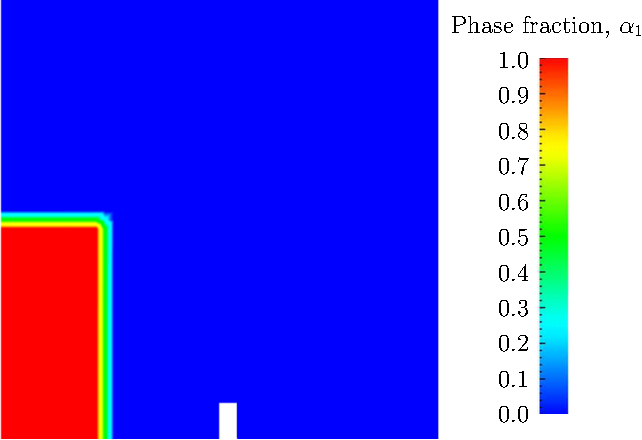
\includegraphics{fig-2-21}
 \caption{相比率\OFkeyword{alpha.water}の初期条件}
 \label{fig:2.21}
\end{figure}


\subsection{流体の物性値}
\label{ssec:2.3.4}
\OFpath{constant}ディレクトリの
\index{transportProperties@\OFpath{transportProperties}!ファイル}%
\index{ファイル!transportProperties@\OFpath{transportProperties}}%
\OFpath{transportProperties}ファイルを確認しましょう.
このディクショナリは各流体の物性値を含んでおり,
二つのディクショナリ\OFsubdictionary{water}と
\OFsubdictionary{air}に分かれています.
各相の輸送モデルは,\OFkeyword{transportModel}によって選択されます.
ここで,動粘性係数が\OFkeyword{nu}というキーワードで指定され,
一定値である
\index{Newtonian@\OFkeyword{Newtonian}!キーワードエントリ}%
\index{キーワードエントリ!Newtonian@\OFkeyword{Newtonian}}%
\OFkeyword{Newtonian}モデルを選んでください.

\index{CrossPowerLaw@\OFkeyword{CrossPowerLaw}!キーワードエントリ}%
\index{キーワードエントリ!CrossPowerLaw@\OFkeyword{CrossPowerLaw}}%
\OFkeyword{CrossPowerLaw}といったその他のモデルにおける粘性係数の指定は,
この例における\OFsubdictionary{CrossPowerLawCoeffs}といったように,
\OFsubdictionary{<model>Coeffs}という名のサブディクショナリの中で行います.

密度の指定は,\OFkeyword{rho}キーワードで行います.

二つの相の間の表面張力は,\OFkeyword{sigma}キーワードで指定します.

このチュートリアルで用いた値を\autoref{tbl:2.3}に挙げます.


\begin{table}
 %#! platex UserGuideJa
\begin{tabular}{lccc}
 \OFkeyword{phase1}の物性 \\
 \hline
 動粘性率 & $\unit*{m^{2}s^{-1}}$ & \OFkeyword{nu} & $1.0 \times 10^{6}$ \\
 密度 & $\unit*{kg\,m^{-3}}$ & \OFkeyword{rho} & $1.0 \times 10^{3}$ \\
 \\
 \OFkeyword{phase2}の物性 \\
 \hline
 動粘性率 & $\unit*{m^{2}s^{-1}}$ & \OFkeyword{nu} & $1.48 \times 10^{-5}$ \\
 密度 & $\unit*{kg\,m^{-3}}$ & \OFkeyword{rho} & $1.0$ \\
 \\
 両相の物性 \\
 \hline
 表面張力 & $\unit*{N\,m^{^1}}$ & \OFkeyword{sigma} & $0.07$ \\
 \hline
\end{tabular}

 \caption{\OFcase{damBreak}チュートリアルにおける流体物性}
 \label{tbl:2.3}
\end{table}


重力加速度は全領域にわたって一様で,
\OFpath{constant}ディレクトリの
\index{g@\OFpath{g}!ファイル}%
\index{ファイル!g@\OFpath{g}}%
\OFpath{g}ファイルで指定されます.
\OFpath{U}や\OFpath{p}のような通常のフィールドのファイルと異なり,
\OFpath{g}は\OFclass{uniformDimensionedVectorField}であり,
単に\OFkeyword{dimensions}と\OFkeyword{value}の組だけを含みます.
このチュートリアルでは$(0, 9.81, 0)\unit{m\,s^{-2}}$です.
\begin{OFverbatim}[file, linenum=17]

dimensions      [0 1 -2 0 0 0 0];
value           ( 0 -9.81 0 );


// ************************************************************************* //
\end{OFverbatim}


\subsection{乱流モデル}
\label{ssec:2.3.5@1.6}
キャビティの例題のように,
\index{turbulenceProperties@\OFdictionary{turbulenceProperties}!ディクショナリ}%
\index{ディクショナリ!turbulenceProperties@\OFdictionary{turbulenceProperties}}%
\OFdictionary{turbulenceProperties}ディクショナリの
\index{simulationType@\OFkeyword{simulationType}!キーワード}%
\index{キーワード!simulationType@\OFkeyword{simulationType}}%
\OFkeyword{simulationType}キーワードで乱流のモデリング手法を選択することができます.
この例題は乱流モデルを使わずに実行したいので\OFkeyword{laminar}と指定します.
\begin{OFverbatim}[file, linenum=17]

simulationType  laminar;


// ************************************************************************* //
\end{OFverbatim}


\subsection{時間ステップの制御}
\label{ssec:2.3.5}
自由界面の捕捉においては,時間ステップの制御は重要です.
というのも,界面捕捉のアルゴリズムは,通常の流体計算に比べ,
Courant数$\nCo$に対してかなり鋭敏だからです.
理想的には,界面がある領域において,
上限値として$\nCo \approx 0.5$を超えないようにすべきです.
伝播速度の予測が容易であるようなケースでは,$\nCo$の制限を守るような
固定した時間ステップを指定することができますが,
より複雑なケースの場合時間ステップの指定はずっと困難になります.
そこで,\OFtool{interFoam}では,\OFdictionary{controlDict}において,
時間ステップの自動修正を指定することをお勧めします.
\index{adjustTimeStep@\OFkeyword{adjustTimeStep}!キーワード}%
\index{キーワード!adjustTimeStep@\OFkeyword{adjustTimeStep}}%
\OFkeyword{adjustTimeStep}を\OFkeyword{on}にして,
$\nCo$の最大値 (相の場については
\index{maxAlphaCo@\OFkeyword{maxAlphaCo}!キーワード}%
\index{キーワード!maxAlphaCo@\OFkeyword{maxAlphaCo}}%
\OFkeyword{maxAlphaCo},その他の場については
\index{maxCo@\OFkeyword{maxCo}!キーワード}%
\index{キーワード!maxCo@\OFkeyword{maxCo}}%
\OFkeyword{maxCo}) を$1.0$にしましょう.
時間ステップの上限
\index{maxDeltaT@\OFkeyword{maxDeltaT}!キーワード}%
\index{キーワード!maxDeltaT@\OFkeyword{maxDeltaT}}%
\OFkeyword{maxDeltaT}は
このシミュレーションでは超えようのない値,
たとえば$1.0$等に設定すればよいでしょう.

ただし,自動時間ステップ制御を用いると,
その時間ステップは必ずしも使いやすい値に丸められるとは限りません.
したがって,固定の時間ステップ間隔でOpenFOAMに結果を出力させた場合,
その時刻はきりの良い値になりません.
ところがこの自動時間ステップ制御を用いていても,
OpenFOAMでは決まった時刻に結果を出力するように指定することが可能です.
この場合,OpenFOAMは,結果の出力に指定された時刻ぴったりに合うように
時間刻みを補正しつつ,自動時間刻みの制御を行います.
これを行うには,\OFdictionary{controlDict}ディクショナリにおける
\index{writeControl@\OFkeyword{writeControl}!キーワード}%
\index{キーワード!writeControl@\OFkeyword{writeControl}}%
\OFkeyword{writeControl}に対して,
\index{adjustableRunTime@\OFkeyword{adjustableRunTime}!キーワードエントリ}%
\index{キーワードエントリ!adjustableRunTime@\OFkeyword{adjustableRunTime}}%
\OFkeyword{adjustableRunTime}オプションを選んでください.
\index{controlDict@\OFdictionary{controlDict}!ディクショナリ}%
\index{ディクショナリ!controlDict@\OFdictionary{controlDict}}%
\OFdictionary{controlDict}ディクショナリの中身は以下のようになります.
\begin{OFverbatim}[file, linenum=17]

application     interFoam;

startFrom       startTime;

startTime       0;

stopAt          endTime;

endTime         1;

deltaT          0.001;

writeControl    adjustableRunTime;

writeInterval   0.05;

purgeWrite      0;

writeFormat     ascii;

writePrecision  6;

writeCompression uncompressed;

timeFormat      general;

timePrecision   6;

runTimeModifiable yes;

adjustTimeStep  yes;

maxCo           1.0;
maxAlphaCo      1.0;

maxDeltaT       1;


// ************************************************************************* //
\end{OFverbatim}


\subsection{離散化スキーム}
\label{ssec:2.3.6}
この\OFtool{interFoam}ソルバは,OpenCFDによって開発された
Multidimensional Universal Limiter for Explicit Solution (MULES) 法を用いており,
基礎を成す数値的スキームやメッシュ構造から
独立な段階分数の有界性を保存するために使います.
したがって,対流項に対するスキームの選択は,
風上差分のように,安定性や有界性の強いものに限定されません.

対流項のスキームは,\OFdictionary{fvSchemes}ディクショナリの
\OFsubdictionary{divSchemes}サブディクショナリで設定します.
この例題では,運動量方程式における対流項$\nabla \cdot (\rho\bm{U}\bm{U})$に対しては,
\OFkeyword{div(rho*phi,U)}キーワードにて,
\OFkeyword{Gauss linearUpwind grad(U)}を使えば良い精度が得られます.
リミッタ付きの線形なスキームでは,
\autoref{ssec:4.4.1}に記述されるように係数$\phi$を必要とします.
ここでは最も安定性が高くなるように$\phi = 1.0$とします%
\footnote{訳注:旧バージョンで\OFkeyword{Gauss limitedLinearV 1.0}が使われていたときの説明が残っているが,
バージョン2.3.0から\OFkeyword{Gauss linearUpwind grad(U)}に変更されたので$\phi = 1.0$は使われない.}%
.
\OFkeyword{div(phi,alpha)}キーワードで表される$\nabla \cdot (\bm{U}\alpha)$項には
\OFkeyword{vanLeer}を使用します.
\OFkeyword{div(phirb,alpha)}キーワードで表される$\nabla \cdot (\bm{U}_{\mathrm{rb}}\alpha)$項には
2次精度の\OFkeyword{linear}(中心)差分を使うと,MULESアルゴリズムによって有界性が保証されます.

その他の離散化項は一般に決ったスキームを使用します.
以上から
\index{fvSchemes@\OFdictionary{fvSchemes}!ディクショナリ}%
\index{ディクショナリ!fvSchemes@\OFdictionary{fvSchemes}}%
\OFdictionary{fvSchemes}ディクショナリのエントリは以下のようになるでしょう.
\begin{OFverbatim}[file, linenum=17]

ddtSchemes
{
    default         Euler;
}

gradSchemes
{
    default         Gauss linear;
}

divSchemes
{
    div(rhoPhi,U)  Gauss linearUpwind grad(U);
    div(phi,alpha)  Gauss vanLeer;
    div(phirb,alpha) Gauss linear;
    div((muEff*dev(T(grad(U))))) Gauss linear;
}

laplacianSchemes
{
    default         Gauss linear corrected;
}

interpolationSchemes
{
    default         linear;
}

snGradSchemes
{
    default         corrected;
}

fluxRequired
{
    default         no;
    p_rgh;
    pcorr;
    alpha.water;
}


// ************************************************************************* //
\end{OFverbatim}


\subsection{線形ソルバの制御}
\label{ssec:2.3.7}
\OFdictionary{fvSolution}では,
\OFsubdictionary{PISO}サブディクショナリが
\OFtool{interFoam}に特化した要素を含んでいます.
ここには,通常と同じく運動量方程式に対する反復数だけでなく,
$\alpha$相方程式のPISOループに対する反復数も指定します.
特に重要なものは\OFkeyword{nAlphaSubCycles}と\OFkeyword{cAlpha}キーワードです.
\index{nAlphaSubCycles@\OFkeyword{nAlphaSubCycles}!キーワード}%
\index{キーワード!nAlphaSubCycles@\OFkeyword{nAlphaSubCycles}}%
\OFkeyword{nAlphaSubCycles}は$\alpha$方程式内の内側反復の数を表してあり,
ここで,内側反復は与えられた時間ステップ内での方程式に対する
付加的な解の点数です.
それは,時間ステップや計算時間の莫大な増加なしで
解を安定させることができるようにするものです.
ここでは,二つのsub-cycleを指定しており,
$\alpha$方程式は実際の各時間ステップ内で2分の1の幅の
時間スッテプで2回解かれていることを意味します.

\index{cAlpha@\OFkeyword{cAlpha}!キーワード}%
\index{キーワード!cAlpha@\OFkeyword{cAlpha}}%
\OFkeyword{cAlpha}キーワードは界面の圧縮を制御する要素です.
つまり,$0$は無圧縮に対応し,$1$は保存的な圧縮に対応し,
$1$以上は拡張された界面の圧縮を意味します.
通常はこの例題で用いられている$1.0$の値が推奨されます.


\subsection{コードの実行}
\label{ssec:2.3.8}
コードの実行方法については,
前述のチュートリアルに詳細に記述しています.
以下のようにして,
標準出力とファイルの両方への書き込みを可能にする
\texttt{tee}コマンドを試してみてください.
\begin{OFverbatim}[terminal]
cd $FOAM_RUN/tutorials/multiphase/interFoam/laminar/damBreak
interFoam | tee log
\end{OFverbatim}%$
このコードは,対話的に実行されつつ,
出力のコピーを\OFpath{log}ファイルに記録してくれます.


\subsection{後処理}
\label{ssec:2.3.9}
結果の後処理は,通常の方法で行えます.
ユーザは参照時間の経過に伴う相比率\OFkeyword{alpha.water}の発達を見ることができます.
例えば\autoref{fig:2.22}をみてください.


\begin{figure}[ht]
 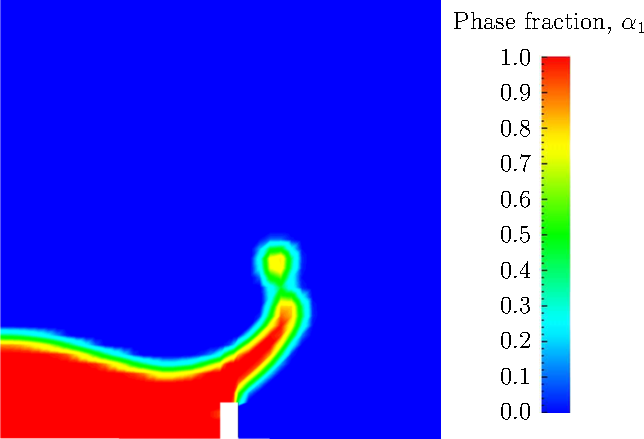
\includegraphics{fig-2-22-a}\par
 (a) $t = 0.25\unit{s}$のとき\par
 \medskip
 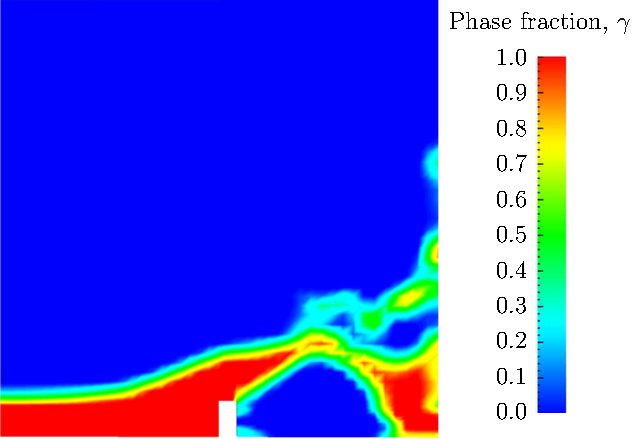
\includegraphics{fig-2-22-b}\par
 (b) $t = 0.50\unit{s}$のとき
 \caption{$\alpha$相のスナップショット}
 \label{fig:2.22}
\end{figure}


\subsection{並列計算}
\label{ssec:2.3.10}
前述の例の結果はかなり目の粗い格子を使って得られました.
ここでは格子の解像度を増やして再計算します.
新しいケースは,一般的に一つのプロセッサでは
計算するのに数時間を要するので,
複数のプロセッサにアクセスしているのであれば,
OpenFOAMの並列計算機能を試してみてもよいでしょう.

まず初めに,\OFcase{damBreak}ケースのコピーをしてください.
\begin{OFverbatim}[terminal]
cd $FOAM_RUN/tutorials/interFoam
mkdir damBreakFine
cp -r damBreak/0 damBreakFine
cp -r damBreak/system damBreakFine
cp -r damBreak/constant damBreakFine
\end{OFverbatim}%$

新しいケースは\OFcase{damBreakFine}と名づけてください.
新しいケースディレクトリを開いて
\OFdictionary{blockMeshDict}ファイル内の
\OFkeyword{blocks}の記述を以下のように変更してください.
\begin{OFverbatim}[file]
blocks
(
    hex (0 1 5 4 12 13 17 16) (46 10 1) simpleGrading (1 1 1)
    hex (2 3 7 6 14 15 19 18) (40 10 1) simpleGrading (1 1 1)
    hex (4 5 9 8 16 17 21 20) (46 76 1) simpleGrading (1 2 1)
    hex (5 6 10 9 17 18 22 21) (4 76 1) simpleGrading (1 2 1)
    hex (6 7 11 10 18 19 23 22) (40 76 1) simpleGrading (1 2 1)
);
\end{OFverbatim}
上記で,入力は\OFdictionary{blockMeshDict}ファイルで表示されているように,
つまりは,格子の密度を変更しなければなりません.
例えば\texttt{46 10 1}という入力や\texttt{1 2 1}という格子幅の勾配の入力のようにです.
正しく入力できたら,メッシュを生成します.

ここで格子が\OFcase{damBreak}の例から変更されると,
時刻\OFpath{0}のディレクトリ内の\OFpath{alpha.water}という相の場を
再初期化しなければなりません.
というのも\OFkeyword{alpha.water}は新しい格子とは合致しない
いくつかの要素を含んでいるからです.
ここで,\OFkeyword{U}や\OFkeyword{p\_rgh}という場は
変更する必要がないことに注意しましょう.
それらは\OFkeyword{uniform}として明記されており
フィールド内の要素の数と独立だからです.
フィールドの初期化はシャープな界面をもつように行いたいものです.
つまり,その要素が$\alpha = 1$または$\alpha = 0$となるようにです.
\OFtool{mapFields}によりフィールドを更新すると,
界面に補間された$0 < \alpha < 1$となる値が生成される可能性があるので,
\OFtool{setFields}ユーティリティを再実行したほうがよいでしょう.
その前に初期条件の一様な$\alpha$のバックアップファイル
\OFpath{0/alpha.water.org}を\OFpath{0/alpha.water}にコピーします.
\begin{OFverbatim}[terminal]
cd $FOAM_RUN/tutorials/interFoam/laminar/damBreakFine
cp -r 0/alpha.water.org 0/alpha.water
setFields
\end{OFverbatim}%$

OpenFOAMで用いられる並列計算の手法はいわゆる領域分割であり,
幾何形状やそれに関連する場が領域ごとに分解されて,
解析のため個々のプロセッサに割り当てられます.
そのため,並列計算を実行するために必要な最初の段階は,
\OFtool{decomposePar}を用いて領域を分解することです.
\OFtool{decomposePar}の設定は\OFpath{system}ディレクトリにある,
\OFdictionary{decomposeParDict}というファイルです.
他のユーティリティ同様,初期状態のファイルが
ユーティリティのソースコードの
ディレクトリ (\OFpath{\$FOAM\_UTILITIES/parallelProcessing/\allowbreak decomposePar}) にあります.

最初の入力の\OFkeyword{numberOfSubdomains}において
何個のサブ領域に分割するかを指定します.
通常はこのケースに利用できるプロセッサの数と対応します.

このチュートリアルでは,分解の手法は\OFkeyword{simple}で,
対応する\OFkeyword{simpleCoeffs}は以下の基準のように編集しましょう.
領域は,$x$,$y$,$z$方向で部分かサブ領域に分けられ,
各方向へのサブ領域の数はベクトル$\bm{n}$として与えられます.
この幾何形状は2次元なので,3番目の方向$z$に分割されることはなく,
それゆえ必ず$n_{z}$は$1$になります.
$n_{x}$と$n_{y}$は$x$,$y$方向の領域の分割数$\bm{n}$を構成し,
$n_{x}$と$n_{y}$の積で表されるサブ領域の数が\OFkeyword{numberOfSubdomain}に指定したものと
等しくなる必要があります.
隣接するサブ領域間のセル面の数を最小にしたほうがよいので,
正方形の幾何形状では,$x$,$y$方向を均等に分割するのが良いでしょう.
\OFkeyword{delta}キーワードは\OFkeyword{0.001}に設定しましょう.

例として,四つのプロセッサで計算を実行するとします.
\OFkeyword{numberOfSubdomain}を4に,$\bm{n} = (2, 2, 1)$に設定します.
\OFdictionary{decomposeParDict}を閉じて,\OFtool{decomposePar}を実行します.
\OFtool{decomposePar}のスクリーンメッセージが確認でき,
分解はプロセッサ間で均等に分配されたと表示されます.

\autoref{sec:3.4}に
並列計算の方法についての詳細があるので参照してください.
このチュートリアルでは並列計算の一例を示しているにすぎません.
openMPIを用いて標準のメッセージパッシングインターフェース (MPI) を
実装しています.
ここでは,テストとしてローカルホストのみの単独ノードで実行します.
\begin{OFverbatim}[terminal]
mpirun -np 4 interFoam -parallel > log &
\end{OFverbatim}
\autoref{ssec:3.4.2}に後述しますが,
ケースが実行されるマシンのホストネームを列記したファイルを作っておけば
ネットワーク上のより多くのノードを使って計算することも可能です.
ケースはバックグラウンドで実行し,
進行状況を\OFpath{log}ファイルで監視するのがよいでしょう.


\begin{figure}[ht]
 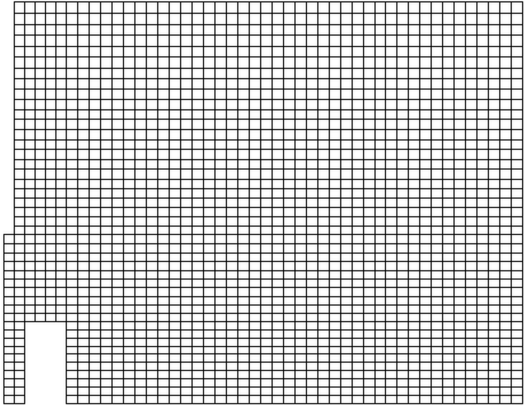
\includegraphics{fig-2-23}
 \caption{並列プロセスケースでのプロセッサ2のメッシュ}
 \label{fig:2.23}
\end{figure}


\begin{figure}[ht]
 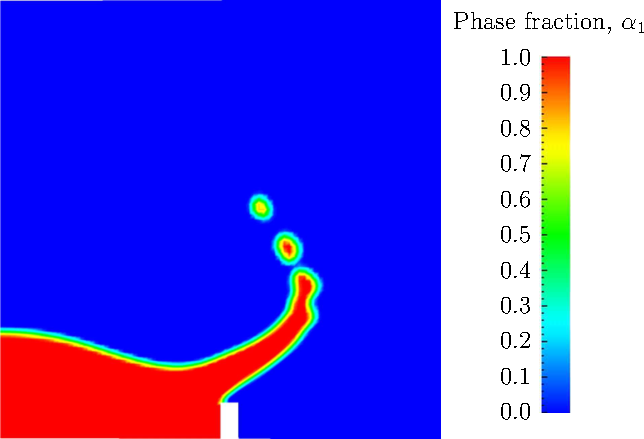
\includegraphics{fig-2-24-a}\par
 (a) $t = 0.25\unit{s}$のとき\par
 \medskip
 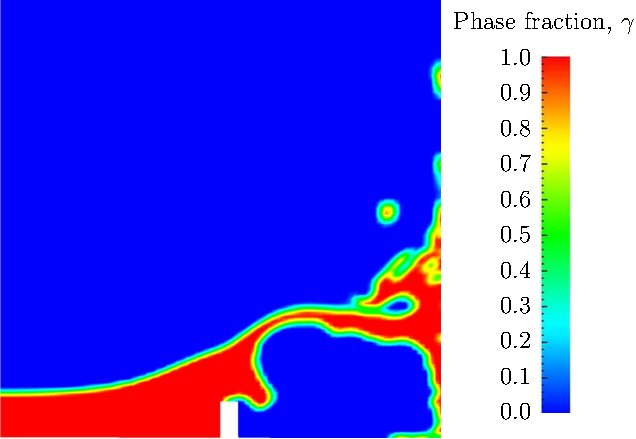
\includegraphics{fig-2-24-b}\par
 (b) $t = 0.50\unit{s}$のとき
 \caption{正確なメッシュの$\alpha$相のスナップショット}
 \label{fig:2.24}
\end{figure}


\subsection{並列計算ケースの後処理}
\label{sssec:2.3.11}
一度ケースの実行が完了したら,
分解されたフィールドとメッシュは\OFtool{reconstructPar}を実行して
後処理のために再統合します.
コマンドラインから容易に実行できます.
細かい格子による結果は\autoref{fig:2.24}に表されます.
インタフェースでの結果は粗い格子のものと比較して
著しく改良されたことがみてとれます.

また,単に個々のプロセッサの領域を一つのケースと扱うことで,
分解された領域の部分を個々に後処理することもできます.

例えば,\OFtool{paraFoam}を以下のように起動します.
\begin{OFverbatim}[terminal]
paraFoam -case processor1
\end{OFverbatim}
すると\OFkeyword{processor1}が\OFthirdparty{ParaView}のケースモジュールとして表れます.
\autoref{fig:2.23}に,\OFkeyword{simple}方式による領域分割を行った際の
\OFkeyword{processor1}のメッシュを示します.

%#! platex UserGuideJa
\chapter{アプリケーションとライブラリ}
\label{chap:3}
\index{OpenFOAM!アプリケーション}%
\index{OpenFOAM!ライブラリ}%
\index{アプリケーション}%
\index{ライブラリ}%
繰り返しいいますが,OpenFOAMは実行のために,
基本的にC++のライブラリを用いています.
OpenFOAMはプリコンパイル済みの数多くのアプリケーションで
構成されていますがユーザが独自に作成したり
従来のものを修正しても構いません.
アプリケーションは大きく二つのカテゴリに分けられています.
\begin{description}
 \item[ソルバ] 数値連続体力学の特定の問題を解くためのもの
 \item[ユーティリティ] 主にデータ操作や代数計算を主に行う
            前後処理を実行するもの
\end{description}
OpenFOAMは一連のプリコンパイル済ライブラリに分けられ,
それらはソルバとユーティリティの集合体をダイナミックにリンクします.
ユーザが適宜独自のモデルをライブラリに追加できるように
物理的モデルのこのようなライブラリはソースコードとして与えられます.

この章ではソルバ,ユーティリティ,ライブラリの概説と
これらの作成,修正,編集,実行方法について述べます.
ソルバとユーティリティのコードの実際の書き方については
ここでは述べませんがプログラマ・ガイドに記載してあります.
なお,プログラマ・ガイドは現在改訂中ですので,
もし何か不明な点がありましたら,
\href{http://www.openfoam.org}{OpenFOAMのウェブサイト}で
新たな情報が得られるかもしれません.



\section{OpenFOAMのプログラミング言語}
\label{sec:3.1}
OpenFOAMライブラリィのはたらきを理解するためには
OpenFOAMの基本言語であるC++の予備知識がいくらか必要となります.
そのために不可欠な知識が本章にあります.
その前に重要なことは,オブジェクト指向プログラミングや
OpenFOAMのメインプログラミング言語としてのC++の選択の背景として
一般論で様々な考えを説明するための言語の概念に着目することです.


\subsection{言語とは}
\label{ssec:3.1.1}
口話と数学が普及には,
特に抽象的な概念を表現する際の効率性が重要でした.

(概念を表現する際の効率性の)例として,流量について,
「速度場 (velocity field)」という言葉を私たちが使うとき,
流れの性質の言及もせず何ら具体的な速度データがなくとも使っています.
その言葉の中には,運動の向きと大きさやその他の
物理的性質との関係の概念が要約されています.
これを数学にすると,「速度場」を$\bm{U}$などの簡易な記号で表し,
また速度場の大きさを表したいときには$|\bm{U}|$として表記します.
数学は口話よりも効率性に優れ,複雑な概念を極めて明快に表現できます.

連続体力学の中で解析しようとしている問題は,
固有の構成要素やタイプとして表現されたものでもなく,
コンピュータの認識する,
いわゆるビット,バイト,数値などの概念とも異なります.
問題はいつも,まず口話で提起され,空間と時間の三次元での
偏微分方程式として表現されます.
それらの方程式はスカラ,ベクトル,テンソル
そしてそれらの場,テンソル代数,テンソル解析,次元の単位などの
概念を含んでおり,これらの解は離散化手法やマトリクス,
ソルバそして解法アルゴリズムを必要とします.
テンソル数学と値計算法については
プログラマ・ガイドの第1\nobreak 章と第2\nobreak 章に記載しています.


\subsection{オブジェクト指向とC++}
\label{ssec:3.1.2}
C++のようなオブジェクト指向のプログラミング言語は,
宣言の型としてクラスという考え方を採用しており,
口語の部分や科学計算や技術計算に用いられる
数学的な言語を取り扱っています.
先に紹介した速度場はプログラミングコードでは記号\texttt{U}で表され,
速度場の大きさは\texttt{mag(U)}で表されます.
速度はベクトル場であり,
オブジェクト指向コードでは\texttt{vectorField}クラスとなります.
速度場\texttt{U}は,オブジェクト指向の項であることから,
この場合\texttt{vectorField}クラスのインスタンス,
あるいはオブジェクトとということになります.

プログラミングの中で,
物理的なオブジェクトと抽象的な構成要素を表現する
オブジェクト指向のもっている明瞭さを過小評価してはいけません.
クラス構造は,クラス自身など,
開発したコードの領域を包含する集合であるから,
容易にコードを管理することができます.
新しいクラスには,他のクラスからのプロパティを
継承させることができることから,
\texttt{vectorField}には\texttt{vector}クラスと
\texttt{Field}クラスを継承させることができます.
C++はテンプレートクラスのメカニズムを備えています.
例えばテンプレートクラス\texttt{Field<Type>}は\texttt{scalar},
\texttt{vector},\texttt{tensor}など
どんな\texttt{<Type>}の\texttt{Field}も表現できます.
テンプレートクラスの一般的な特性はテンプレートから作成される
どんなクラスにも通じます.
テンプレート化や継承はコードの重複を減らし,
コードの全体構造を決めるクラスのヒエラルキを作ります.


\subsection{方程式の説明}
\label{ssec:3.1.3}
OpenFOAMの設計の中心的なテーマは,
OpenFOAMのクラスを用いて書かれたソルバのアプリケーションであり,
偏微分方程式の解法と非常に似た構造をもっています.例えば方程式
\begin{align*}
 \frac{\partial\rho\bm{U}}{\partial t} + \nabla \cdot \phi\bm{U}
 - \nabla \cdot \mu\nabla\bm{U} = -\nabla p
\end{align*}
はコード
\begin{OFverbatim}[file]
solve
(
    fvm::ddt(rho, U)
  + fvm::div(phi, U)
  - fvm::laplacian(mu, U)
    ==
  - fvc::grad(p)
);
\end{OFverbatim}
で表されます.

これらの必要条件として,
OpenFOAMの主たるプログラミング言語が継承やテンプレートクラス,
仮想関数,演算子の多重定義といったオブジェクト指向的特徴を
もっていることが必要です.
これらの特性は,Fortran~90のようにオブジェクト指向と称しつつ
実際には非常に限られたオブジェクト指向の能力しか
もっていない多くの言語では十分に利用できません.
しかし,C++はこれらの特性をすべてもつうえに,
効率性の良い実行ファイルを作り出す信頼性のあるコンパイラを
使えるように標準的な仕様が定められたうえで広く使われている
というさらなる長所をもっています.
ゆえにOpenFOAMの主要言語なのです.


\subsection{ソルバコード}
\label{ssec:3.1.4}
ソルバコードは,解法アルゴリズムと方程式の手続き上の
説明のようなものなので当然のようにほとんど手続きです.
オブジェクト指向やソルバを書くための
C++プログラミングへの深い知識は必要ありませんが,
オブジェクト指向やクラスの原理やいくらかC++コードの
構文の基礎知識は知っておくべきでしょう.
基礎的な方程式やモデルや解法の理解やアルゴリズムは非常に重要です.

ユーザはたいていの場合OpenFOAMクラスのどんなコードでも
深く考える必要はありません.
オブジェクト指向の真髄はユーザが何もしなくてもよいところにあります.
単にクラスの在り方と機能の知識だけでクラスを使うのに十分です.
それぞれのクラスやその機能などの説明は,
OpenFOAMの配布物の中にDoxygenで生成されたHTMLのドキュメントとして
供給されており,
\OFpath{\$WM\_PROJECT\_DIR/doc/\allowbreak Doxygen/html/index.html}にあります.



\section{アプリケーションやライブラリのコンパイル}
\label{sec:3.2}
コンパイルはアプリケーションの開発には必要不可欠の部分であり,
各々のコードのピースがそれ自身,
OpenFOAMのライブラリに依存している
コンポーネントにアクセスすることから,
細心の管理が必要となります.
多くの場合,これらの構築はUNIX/Linuxシステムでは
標準のUNIX
\index{make@\OFtool{make}!スクリプト/エイリアス}%
\index{スクリプト/エイリアス!make@\OFtool{make}}%
\OFtool{make}ユーティティを使ってコンパイルします.
しかしながら,OpenFOAMはより用途が広く簡便性に優れている,
\index{wmake@\OFtool{wmake}!スクリプト/エイリアス}%
\index{スクリプト/エイリアス!wmake@\OFtool{wmake}}%
\OFtool{wmake}でのコンパイルスクリプトを提供しています.
実際,\OFtool{wmake}はOpenFOAMのライブラリだけでなく,
どのコードにも使われています.
コンパイルのプロセスを理解するために,
最初にC++のある側面とそのファイル構成について
\autoref{fig:3.1}で説明します.
クラスとは,オブジェクトの構築様式,
データの格納およびクラスのメンバ関数のような
命令文のセットで定義されるものです.
クラスの定義を含むファイルは\OFpath{.C}の拡張子をもっており,
例えばクラスncであればファイル\OFpath{nc.C}と書かれます.
このファイルは,他のコードとは独立にコンパイルして
\OFpath{nc.so}のような拡張子\OFpath{.so}をもつ
オブジェクトライブラリとして知られる
バイナリ実行ライブラリファイルとすることができます.
コードの一部を,仮に\OFpath{newApp.C}などとしてコンパイルするとき,
ユーザーはncクラスを使うことにより,
\OFpath{nc.C}を再コンパイルしなくても
ランタイムとして\OFpath{newApp.C}で\OFpath{nc.so}を
呼び出せばよいことになります.
これがダイナミックリンクといわれるものです.


\begin{figure}[ht]
 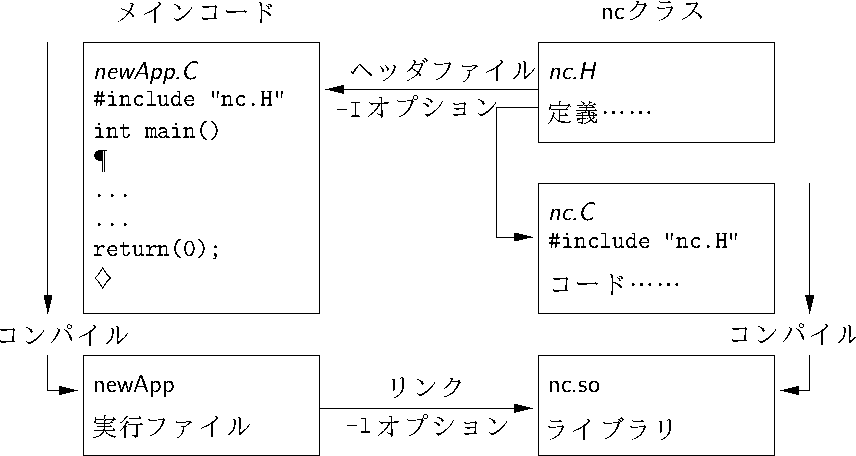
\includegraphics{fig-3-1}
 \caption{ヘッダファイル,ソースファイル,コンパイル,リンク}
 \label{fig:3.1}
\end{figure}


\subsection{ヘッダ\OFpath{.H}ファイル}
\label{ssec:3.2.1}
エラーチェックをおこなうにあたって,
コンパイルするコードの部分がどのクラスで用いられるか,
また実際の操作でどのように振舞うかを認識しなければなりません.
それゆえ,(例えば\OFpath{nc.H}のような) \OFpath{.H}ファイル拡張子をもつ
ヘッダファイルによってクラス宣言が必要です.
このようなヘッダファイルにはクラス名とその機能が記述されています.

このファイルは,クラスを用いるあらゆるコード
(クラス宣言のためのコードも含め)の最初の部分に置きます.
\OFpath{.C}コードではどの部分でいくつのクラスを用いてもかまいませんが,
かならずクラス宣言のために\OFpath{.H}ファイルではじめる必要があります.
クラスは他のクラスのリソースとして使うことができますが,
その場合も関連付けた\OFpath{.H}ファイルではじめます.
クラスヒエラルキを再帰的に検索することで,
結局,上位\OFpath{.C}コードが
\index{いぞん@依存}%
依存しているクラス
(これらの\OFpath{.H}ファイルはdependencyとよばれる) で,
すべてのクラスに関するヘッダファイルのリストを
コンパイルすることができます.
\index{いぞんリスト@依存リスト}%
依存リストがあればコンパイラはソースファイルが
最終コンパイル以来アップデートされているかどうかチェックでき,
選択的に必要な部分だけコンパイルできます.

ヘッダファイルは,例えば
\begin{OFverbatim}[file]
# include "otherHeader.H";
\end{OFverbatim}
のような\ 
\index{# include@\verb+# include+!C++こうぶん@C++構文}%
\index{C++こうぶん@C++構文!# include@\verb+# include+}%
\verb|# include|命令文を使ったコードに含まれていますが,
このようなコードはコンパイラに特定のファイルを読ませるために
現在のファイルの読み込みを一時中断させます.
すべての内蔵コードはヘッダファイルに入れること,
コード可読性を高めるためにメインコードにrelevant locationに
含めることができます.
例えば多くのOpenFOAMアプリケーションでは,
作成フィールドや読み込みフィールドの入力データのコードはコードの始めに
\OFpath{createFields.H}と名づけられたファイルに含まれます.
この方法では,ヘッダファイルは単独でクラスの宣言として
使われるだけではありません.
以下のようなその他の機能とともに依存リストファイルを
維持管理するタスクを実行するのが\OFtool{wmake}なのです.
\begin{itemize}
 \item ソースファイルと,それらが依存しているファイルの
       依存関係リストの自動作成と管理
 \item マルチ・プラットフォームコンパイル適切なディレクトリ構造を通じて
       ハンドルされたマルチプラットフォームでのコンパイルとリンク
 \item マルチ・ランゲージコンパイルとCやC++やJava等のリンケージ
 \item CやC++,Javaのようなマルチ言語でのコンパイルとリンク
 \item デバッグや最適化,並列処理,分析といった
       マルチオプションでのコンパイルとリンク
 \item lex,yacc,IDL,MOCといった,ソースコードの作成プログラムのサポート
 \item ソースファイルリストの簡潔なシンタックス
 \item 新規のコードリストのソースファイルリストの自動生成
 \item 多重分割あるいは静的ライブラリの簡潔なハンドリング
 \item 新しいタイプのマシンへの拡張性
 \item \texttt{make};\texttt{sh},\texttt{ksh}または\texttt{csh};
       \texttt{lex},\texttt{cc}をもついかなるマシンでの
       作業に対する優れた移植性
 \item Apollo,SUN,SGI,HP (HPUX),Compaq (DEC),IBM (AIX),Cray,Ardent,
       Stardent,PC Linux,PPC Linux,NEC,SX4,Fujitsu VP1000での動作確認
\end{itemize}


\subsection{\OFtool{wmake}によるコンパイル}
\label{ssec:3.2.2}
OpenFOAMのアプリケーションは各アプリケーションのソースコードが
そのアプリケーション名のディレクトリに置かれるという
一般的決まりで編成されます.
最上位ソースファイルはアプリケーション名に拡張子\OFpath{.C}をつけます.
例えば,newAppというアプリケーションのソースコードは
\autoref{fig:3.2}に示すようにnewAppのディレクトリに存在し,
最上位ファイルは\OFpath{newApp.C}となります.


\begin{figure}[ht]
 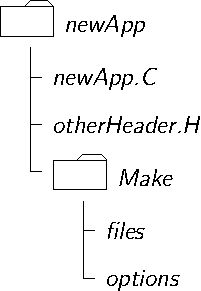
\includegraphics{fig-3-2}
 \caption{アプリケーションのディレクトリ構成}
 \label{fig:3.2}
\end{figure}


ディレクトリは
\index{options@\OFpath{options}!ファイル}%
\index{ファイル!options@\OFpath{options}}%
\OFpath{options}と
\index{files@\OFpath{files}!ファイル}%
\index{ファイル!files@\OFpath{files}}%
\OFpath{files}の二つのファイルを含んだ
\index{Make@\OFpath{Make}!ディレクトリ}%
\index{ディレクトリ!Make@\OFpath{Make}}%
\OFpath{Make}というサブディレクトリももっており,それについては次節で述べます.

\subsubsection{ヘッダの読み込み}
\label{sssec:3.2.2.1}
コンパイラは,以下の順で
\OFtool{wmake}で\verb|−I|オプションが指定されたヘッダファイルを検索します.
\begin{enumerate}
 \item \OFpath{\$WM\_PROJECT\_DIR/src/OpenFOAM/lnInclude}ディレクトリ
 \item \OFpath{newApp/lnInclude}のようなローカルディレクトリ
 \item \OFpath{newApp}のようなローカルディレクトリ
 \item \OFpath{/usr/X11/include}や\OFpath{\$(MPICH\_ARCH\_PATH)/include}のように,
\index{wmake@\OFtool{wmake}!プラットフォーム}%
       プラットフォームに依存する
       \OFpath{\$WM\_PROJECT\_DIR/wmake/rules/\$WM\_ARCH/}ディレクトリの中の
       ファイルに設定されているパス
 \item \verb|-I|オプションをもつ\OFpath{Make/options}ファイルの中で
       明確に指定されている他のディレクトリ
\end{enumerate}
\OFpath{Make/options}ファイルは構文を使っているヘッダファイルを
配置するためのフルディレクトリパスを含みます.
\begin{OFverbatim}[file]
EXE_INC = \
    -I<directoryPath1> \
    -I<directoryPath2> \
    ...                \
    -I<directoryPathN>
\end{OFverbatim}
ディレクトリ名は頭に\verb|-I|をつけ,
各行では\verb|EXE_INC|を続けるために構文は\verb|\|を使い,
最終記入後は\verb|\|をつけないことに注意してください.

\subsubsection{ライブラリへのリンク}
\label{sssec:3.2.2.2}
コンパイラは,以下の\OFtool{wmake}の\verb|-L|オプションで指定された
ディレクトリパスのオブジェクトライブラリファイルにリンクします.
\begin{enumerate}
 \item \OFpath{\$FOAM\_LIBBIN}ディレクトリ
 \item \OFpath{\$WM\_DIR/rules/\$WM\_ARCH/}デイレクトリの中に設定された
       機種に依存するパス,例えば,\OFpath{/usr/X11/}や\OFpath{\$(MPICH\_ARCH\_PATH)/lib}
 \item \OFpath{Make/options}ファイルで指定された他のディレクトリ
\end{enumerate}
リンクされる実際のライブラリファイルは\verb|-l|オプションで指定し,
接頭辞\OFpath{lib},ライブラリファイルの拡張子\OFpath{.so}を
外さなければなりません.
例えばライブラリ\OFpath{libnew.so}はフラグ\verb|-lnew|に含まれます.

デフォルトでは,\OFtool{wmake}は以下のライブラリをロードするようになっています
\begin{enumerate}
 \item \OFpath{\$FOAM\_LIBBIN}ディレクトリからの\OFpath{libOpenFOAM.so}ライブラリ
 \item \OFpath{\$WM\_DIR/rules/\$WM\_ARCH/}ディレクトリの中のファイルに設定された
       機種に依存するライブラリ,
       例えば,\OFpath{/usr/X11/lib}における\OFpath{libm.so}や,
       \OFpath{\$(LAM ARCH PATH)/lib}における\OFpath{liblam.so}
 \item \OFpath{Make/options}ファイルで指定された他のライブラリ
\end{enumerate}
\OFpath{Make/options}ファイルは構文を使っているヘッダファイルを
おくための全ディレクトリパスを含みます.
\begin{OFverbatim}[file]
EXE_LIBS = \
    -L<libraryPath1> \
    -L<libraryPath2> \
    ...              \
    -L<libraryPathN> \
    -l<library1>     \
    -l<library2>     \
    ...              \
    -l<libraryN>
\end{OFverbatim}
繰り返しになりますが,ディレクトリパスは頭に\verb|-L|フラグを付け,
ライブラリ名は頭に\verb|-l|フラグをつけます.

\subsubsection{コンパイルすべきソースファイル}
\label{sssec:3.2.2.3}
コンパイラはコンパイルすべき\OFpath{.C}ソースファイルのリストが必要です.
リストはメインの\OFpath{.C}ファイルだけではなく
特定のアプリケーションのために生成されるがクラスライブラリの中に
含まれない他のソースファイルも含まれなければなりません.
例えば,新しいクラスを作成したり,
特定のアプリケーション用のクラスに
新しい機能をつけくわえることができます.
\OFpath{.C}ソースファイルのフルリストは
\index{Make/files@\OFpath{Make/files}!ファイル}%
\index{ファイル!Make/files@\OFpath{Make/files}}%
\OFpath{Make/files}ファイルに
含む必要があります.当然,アプリケーションは多くなるので,
フルリストには (例えば前述のアプリケーション例における
\OFpath{newApp.C}のような) メイン\OFpath{.C}ファイルの名前だけを入れます.
\OFpath{Make/files}ファイルは\verb|EXE =|構文によって
指定されたコンパイル済み実行ファイルの名前とフルパスも含みます.
一般的な決まりではnewAppのようにアプリケーション名をつけることが
規定されています.
OpenFOAMのリリースにはパスのために便利な二つの選択肢があります.
標準的なリリースではアプリケーションは\OFpath{\$FOAM\_APPBIN}に
保存されますが,ユーザにより開発されたアプリケーションは
\OFpath{\$FOAM\_USER\_APPBIN}に保存されます.

もしアプリケーションを開発したら,
個人のOpenFOAMアプリケーションのためのソースコードを含む
\OFpath{\$WM\_PROJECT\_USER\_DIR}ディレクトリに
アプリケーションサブディレクトリを作ることをお薦めします.
スタンダードアプリケーションと同様に
各OpenFOAMアプリケーションのソースコードも
各ディレクトリ内に保存しておいてください.
ユーザーアプリケーションとスタンダードリリースのものの違いは
\OFpath{Make/files}ファイルが\OFpath{\$FOAM\_USER\_APPBIN}ディレクトリ内に
書き込まれている実行可能ファイルを指定していることだけです.
例としての\OFpath{Make/files}を以下に記載します.
\begin{OFverbatim}[file]
newApp.C

EXE = $(FOAM_USER_APPBIN)/newApp
\end{OFverbatim}%$

\subsubsection{\OFtool{wmake}の実行}
\label{sssec:3.2.2.4}
\OFtool{wmake}のスクリプトは以下のように入力することで実行されます.
\begin{OFverbatim}[terminal]
wmake <optionalArguments> <optionalDirectory>
\end{OFverbatim}
\verb|<optionalDirectory>| はコンパイルしようとしているアプリケーションの
ディレクトリパスです.
通常,\verb|<optionalDirectory>| が省略可能な場合には
\OFtool{wmake}はコンパイル中のアプリケーションのディレクトリ内から実行されます.


アプリケーションファイルを作成したい場合には
\verb|<optionalArguments>|は必要ありません.
しかし\verb|<optionalArguments>|は\autoref{tbl:3.1}に示すように
ライブラリ等の作成の際には指定されることになります.


\begin{table}[ht]
 %#! platex UserGuideJa
\begin{tabular}{ll}
 Argument & コンパイルの種類 \\
 \hline
 \tblstrut
 \texttt{lib} & 静的にリンクされたライブラリの作成 \\
 \texttt{libso} & 動的にリンクされたライブラリの作成 \\
 \texttt{libo} & 静的にリンクされたオブジェクトファイルライブラリの作成 \\
 \texttt{jar} & JAVAアーカイブの作成 \\
 \texttt{exe} & 特定のプロジェクトから独立したアプリケーションの作成 \\
 \hline
\end{tabular}

 \caption{\OFtool{wmake}のコンパイルオプション}
 \label{tbl:3.1}
\end{table}


\subsubsection{\OFtool{wmake}の環境変数}
\label{sssec:3.2.2.5}
参考として,\OFtool{wmake}で使われる環境変数の設定を
\autoref{tbl:3.2}に示します.


\begin{table}[ht]
 %#! platex UserGuideJa
\begin{tabularx}{\textwidth}{lX}
 主なパス & \\
 \hline
\index{WM PROJECT INST DIR@\string\OFenv{WM\_PROJECT\_INST\_DIR}!かんきょうへんすう@環境変数}%
\index{かんきょうへんすう@環境変数!WM PROJECT INST DIR@\string\OFenv{WM\_PROJECT\_INST\_DIR}}%
 \OFenv{\$WM\_PROJECT\_INST\_DIR}
 & インストールディレクトリへのフルパス,例:\OFpath{\$HOME/OpenFOAM} \\
\index{WM PROJECT@\string\OFenv{WM\_PROJECT}!かんきょうへんすう@環境変数}%
\index{かんきょうへんすう@環境変数!WM PROJECT@\string\OFenv{WM\_PROJECT}}%
 \OFenv{\$WM\_PROJECT}
 & コンパイルされたプロジェクトの名前:\texttt{OpenFOAM} \\
\index{WM PROJECT VERSION@\string\OFenv{WM\_PROJECT\_VERSION}!かんきょうへんすう@環境変数}%
\index{かんきょうへんすう@環境変数!WM PROJECT VERSION@\string\OFenv{WM\_PROJECT\_VERSION}}%
 \OFenv{\$WM\_PROJECT\_VERSION}
 & コンパイルされたプロジェクトのバージョン:\texttt{\OFversion} \\
\index{WM PROJECT DIR@\string\OFenv{WM\_PROJECT\_DIR}!かんきょうへんすう@環境変数}%
\index{かんきょうへんすう@環境変数!WM PROJECT DIR@\string\OFenv{WM\_PROJECT\_DIR}}%
 \OFenv{\$WM\_PROJECT\_DIR}
 & OpenFOAMのバイナリ実行ファイル置き場へのフルパス,\hfil\break
     例:\OFpath{\$HOME/OpenFOAM/OpenFOAM-\OFversion} \\
\index{WM PROJECT USER DIR@\string\OFenv{WM\_PROJECT\_USER\_DIR}!かんきょうへんすう@環境変数}%
\index{かんきょうへんすう@環境変数!WM PROJECT USER DIR@\string\OFenv{WM\_PROJECT\_USER\_DIR}}%
 \OFenv{\$WM\_PROJECT\_USER\_DIR}
 & ユーザのバイナリ実行ファイル置き場へのフルパス,\hfil\break
     例:\OFpath{\$HOME/OpenFOAM/\${USER}-\OFversion} \\
 \\
 その他のパスと設定 & \\
 \hline
\index{WM ARCH@\string\OFenv{WM\_ARCH}!かんきょうへんすう@環境変数}%
\index{かんきょうへんすう@環境変数!WM ARCH@\string\OFenv{WM\_ARCH}}%
 \OFenv{\$WM\_ARCH}
 & マシン・アーキテクチャ:
     \texttt{Linux}, \texttt{SunOS} \\
\index{WM ARCH OPTION@\string\OFenv{WM\_ARCH\_OPTION}!かんきょうへんすう@環境変数}%
\index{かんきょうへんすう@環境変数!WM ARCH OPTION@\string\OFenv{WM\_ARCH\_OPTION}}%
 \OFenv{\$WM\_ARCH\_OPTION}
 & \texttt{32}あるいは\texttt{64}ビットのアーキテクチャ \\
\index{WM COMPILER@\string\OFenv{WM\_COMPILER}!かんきょうへんすう@環境変数}%
\index{かんきょうへんすう@環境変数!WM COMPILER@\string\OFenv{WM\_COMPILER}}%
 \OFenv{\$WM\_COMPILER}
 & 使用するコンパイラ:\texttt{Gcc45} - \textsf{gcc} 4.5+, \texttt{ICC} - Intel \\
\index{WM COMPILER DIR@\string\OFenv{WM\_COMPILER\_DIR}!かんきょうへんすう@環境変数}%
\index{かんきょうへんすう@環境変数!WM COMPILER DIR@\string\OFenv{WM\_COMPILER\_DIR}}%
 \OFenv{\$WM\_COMPILER\_DIR}
 & コンパイラインストールディレクトリ \\
\index{WM COMPILER BIN@\string\OFenv{WM\_COMPILER\_BIN}!かんきょうへんすう@環境変数}%
\index{かんきょうへんすう@環境変数!WM COMPILER BIN@\string\OFenv{WM\_COMPILER\_BIN}}%
 \OFenv{\$WM\_COMPILER\_BIN}
 & コンパイラインストールバイナリ:\OFpath{\$WM\_COMPILER\_BIN/bin} \\
\index{WM COMPILER LIB@\string\OFenv{WM\_COMPILER\_LIB}!かんきょうへんすう@環境変数}%
\index{かんきょうへんすう@環境変数!WM COMPILER LIB@\string\OFenv{WM\_COMPILER\_LIB}}%
 \OFenv{\$WM\_COMPILER\_LIB}
 & コンパイラインストールライブラリ:\OFpath{\$WM\_COMPILER\_BIN/lib} \\
\index{WM COMPILE OPTION@\string\OFenv{WM\_COMPILE\_OPTION}!かんきょうへんすう@環境変数}%
\index{かんきょうへんすう@環境変数!WM COMPILE OPTION@\string\OFenv{WM\_COMPILE\_OPTION}}%
 \OFenv{\$WM\_COMPILE\_OPTION}
 & コンパイルオプション:\texttt{Debug} - debugging, \texttt{Opt} optimisation. \\
\index{WM DIR@\string\OFenv{WM\_DIR}!かんきょうへんすう@環境変数}%
\index{かんきょうへんすう@環境変数!WM DIR@\string\OFenv{WM\_DIR}}%
 \OFenv{\$WM\_DIR}
 & wmakeディレクトリのフルパス \\
\index{WM MPLIB@\string\OFenv{WM\_MPLIB}!かんきょうへんすう@環境変数}%
\index{かんきょうへんすう@環境変数!WM MPLIB@\string\OFenv{WM\_MPLIB}}%
 \OFenv{\$WM\_MPLIB}
 & 並列通信ライブラリ:\texttt{LAM},\texttt{MPI},\texttt{MPICH},\texttt{PVM} \\
\index{WM OPTIONS@\string\OFenv{WM\_OPTIONS}!かんきょうへんすう@環境変数}%
\index{かんきょうへんすう@環境変数!WM OPTIONS@\string\OFenv{WM\_OPTIONS}}%
 \OFenv{\$WM\_OPTIONS}
 & $=$ \OFenv{\$WM\_ARCH\$WM\_COMPILER...}\hfill\break
     \null\hfill\OFenv{...\$WM\_COMPILE\_OPTION\$WM\_MPLIB},\break
     例:\texttt{linuxGcc3OptMPICH} \\
\index{WM PRECISION OPTION@\string\OFenv{WM\_PRECISION\_OPTION}!かんきょうへんすう@環境変数}%
\index{かんきょうへんすう@環境変数!WM PRECISION OPTION@\string\OFenv{WM\_PRECISIO\_OPTION}}%
 \OFenv{\$WM\_PRECISION\_OPTION}
 & コンパイルされたバイナリの精度,\texttt{SP}なら単精度,もしくは,\texttt{DP}なら倍精度 \\
 \hline
\end{tabularx}

 \caption{\OFtool{wmake}の環境変数の設定}
 \label{tbl:3.2}
\end{table}


\subsection{依存リストの削除:\OFtool{wclean}と\OFtool{rmdepall}}
\label{ssec:3.2.3}
実行に際して,例題における\OFpath{newApp.dep}のように,
\OFtool{wmake}は拡張子として\OFpath{.dep}をもった依存関係のリストファイルを構築し,
\OFpath{Make/\$WM\_OPTIONS}ディレクトリの中にファイルのリストを格納します.
コードを変更してmakeした後などこれらファイルを除去したい場合には,
\index{wclean@\OFtool{wclean}!スクリプト/エイリアス}%
\index{スクリプト/エイリアス!wclean@\OFtool{wclean}}%
\OFtool{wclean}を入力してスクリプトを実行します.
\begin{OFverbatim}[terminal]
wclean <optionalArguments> <optionalDirectory>
\end{OFverbatim}
さらに,\verb|<optionalDirectory>|はコンパイルされるアプリケーションの
ディレクトリへのパスです.
通常,パスが省略できる場合にはwcleanはアプリケーションの
ディレクトリ範囲内で実行されます.
もし\OFpath{Make}ディレクトリから依存ファイルとファイルを削除したい場合には,
\verb|<optionalArguments>|は必要ありません.
しかしもしlibが\verb|<optionalArguments>|に指定されていたら
ローカルの\OFpath{InInclude}ディレクトリも削除される必要があります.

追加のスクリプト,
\index{rmdepall@\OFtool{rmdepall}!スクリプト/エイリアス}%
\index{スクリプト/エイリアス!rmdepall@\OFtool{rmdepall}}%
\OFtool{rmdepall}は実行時に,
再帰的にディレクトリツリー下の依存関係にあるすべての
\OFpath{.dep}ファイルを除去します.
これはOpenFOAMのライブラリが更新されたときには有効な方法です.


\subsection{コンパイルの例:pisoFoamアプリケーション}
\label{ssec:3.2.4}
アプリケーション\OFtool{pisoFoam}のソースコードは
\OFpath{\$FOAM\_APP/solvers/incompressible/pisoFoam}ディレクトリ内にあり,
最上位ソースファイルは\OFpath{pisoFoam.C}という名前です.
\OFpath{pisoFoam.C}ソースコードは
\begin{OFverbatim}[file, linenum]
/*---------------------------------------------------------------------------*\
  =========                 |
  \\      /  F ield         | OpenFOAM: The Open Source CFD Toolbox
   \\    /   O peration     |
    \\  /    A nd           | Copyright (C) 1991-2009 OpenCFD Ltd.
     \\/     M anipulation  |
-------------------------------------------------------------------------------
License
    This file is part of OpenFOAM.

    OpenFOAM is free software; you can redistribute it and/or modify it
    under the terms of the GNU General Public License as published by the
    Free Software Foundation; either version 2 of the License, or (at your
    option) any later version.

    OpenFOAM is distributed in the hope that it will be useful, but WITHOUT
    ANY WARRANTY; without even the implied warranty of MERCHANTABILITY or
    FITNESS FOR A PARTICULAR PURPOSE.  See the GNU General Public License
    for more details.

    You should have received a copy of the GNU General Public License
    along with OpenFOAM; if not, write to the Free Software Foundation,
    Inc., 51 Franklin St, Fifth Floor, Boston, MA 02110-1301 USA

Application
    pisoFoam

Description
    Transient solver for incompressible flow.

    Turbulence modelling is generic, i.e. laminar, RAS or LES may be selected.

\*---------------------------------------------------------------------------*/

#include "fvCFD.H"
#include "singlePhaseTransportModel.H"
#include "turbulenceModel.H"

// * * * * * * * * * * * * * * * * * * * * * * * * * * * * * * * * * * * * * //

int main(int argc, char *argv[])
{
    #include "setRootCase.H"

    #include "createTime.H"
    #include "createMesh.H"
    #include "createFields.H"
    #include "initContinuityErrs.H"

    // * * * * * * * * * * * * * * * * * * * * * * * * * * * * * * * * * * * //

    Info<< "\nStarting time loop\n" << endl;

    while (runTime.loop())
    {
        Info<< "Time = " << runTime.timeName() << nl << endl;

        #include "readPISOControls.H"
        #include "CourantNo.H"

        // Pressure-velocity PISO corrector
        {
            // Momentum predictor

            fvVectorMatrix UEqn
            (
                fvm::ddt(U)
              + fvm::div(phi, U)
              + turbulence->divDevReff(U)
            );

            UEqn.relax();

            if (momentumPredictor)
            {
                solve(UEqn == -fvc::grad(p));
            }

            // --- PISO loop

            for (int corr=0; corr<nCorr; corr++)
            {
                volScalarField rUA = 1.0/UEqn.A();

                U = rUA*UEqn.H();
                phi = (fvc::interpolate(U) & mesh.Sf())
                    + fvc::ddtPhiCorr(rUA, U, phi);

                adjustPhi(phi, U, p);

                // Non-orthogonal pressure corrector loop
                for (int nonOrth=0; nonOrth<=nNonOrthCorr; nonOrth++)
                {
                    // Pressure corrector

                    fvScalarMatrix pEqn
                    (
                        fvm::laplacian(rUA, p) == fvc::div(phi)
                    );

                    pEqn.setReference(pRefCell, pRefValue);

                    if
                    (
                        corr == nCorr-1
                     && nonOrth == nNonOrthCorr
                    )
                    {
                        pEqn.solve(mesh.solver("pFinal"));
                    }
                    else
                    {
                        pEqn.solve();
                    }

                    if (nonOrth == nNonOrthCorr)
                    {
                        phi -= pEqn.flux();
                    }
                }

                #include "continuityErrs.H"

                U -= rUA*fvc::grad(p);
                U.correctBoundaryConditions();
            }
        }

        turbulence->correct();

        runTime.write();

        Info<< "ExecutionTime = " << runTime.elapsedCpuTime() << " s"
            << "  ClockTime = " << runTime.elapsedClockTime() << " s"
            << nl << endl;
    }

    Info<< "End\n" << endl;

    return 0;
}


// ************************************************************************* //
\end{OFverbatim}
コードはアプリケーションを説明している記述で始まり,
この中で1行の
\index{コメント}%
コメントは\ 
\index{//@\verb+//+!C++こうぶん@C++構文}%
\index{C++こうぶん@C++構文!//@\verb+//+}%
\verb|//| で,
複数行にわたる
\index{コメント}%
コメントは\ 
\index{/*...*/@\verb+/*...*/+!C++こうぶん@C++構文}%
\index{C++こうぶん@C++構文!/*...*/@\verb+/*...*/+}%
\verb|/*...*/| で記述されます.それに続き,
コードはコンパイラに現在のファイルの読み込みを一時停止させ,
\OFpath{pisoFoam.C}に\OFpath{fvCFD.H}を読み込ませるための
例えば\verb|#include "fvCFD.H"|のような
様々な\ 
\index{# include@\verb+# include+!C++こうぶん@C++構文}%
\index{C++こうぶん@C++構文!# include@\verb+# include+}%
\verb|# include|命令文を含んでいます.

\OFtool{pisoFoam}は\OFtool{cfdTools}や\OFtool{incompressibleRASModels}や
\OFemph{incompressibleTransportModels}ライブラリを提供し,
それゆえ\verb|EXE_INC = -I...|オプションとライブラリにリンクする
\verb|EXE_LIBS = -l...|オプションにより
指定されるヘッダファイルが必要となります.
\OFpath{Make/options}はそれゆえ以下のようになります.
\begin{OFverbatim}[file, linenum]
EXE_INC = \
    -I$(LIB_SRC)/turbulenceModels/incompressible/turbulenceModel \
    -I$(LIB_SRC)/transportModels \
    -I$(LIB_SRC)/transportModels/incompressible/singlePhaseTransportModel \
    -I$(LIB_SRC)/finiteVolume/lnInclude

EXE_LIBS = \
    -lincompressibleRASModels \
    -lincompressibleLESModels \
    -lincompressibleTransportModels \
    -lfiniteVolume \
    -lmeshTools
\end{OFverbatim}
\OFtool{pisoFoam}は\OFpath{pisoFoam.C}ソースしか含まず,
実行ファイルはすべての標準的なアプリケーションと同様に
\OFpath{\$FOAM\_APPBIN}に書き込まれます.
\OFpath{Make/files}はそれゆえ以下のようになります.
\begin{OFverbatim}[file, linenum]
pisoFoam.C

EXE = $(FOAM_APPBIN)/pisoFoam
\end{OFverbatim}%$
\OFpath{\$FOAM\_CFD/pisoFoam}ディレクトリで\verb|wmake|とタイプすれば
\OFtool{pisoFoam}をコンパイルできます.

コードはコンパイルされ以下のようなメッセージをが作成されます.
\begin{OFverbatim}[file]
Making dependency list for source file pisoFoam.C
SOURCE DIR=.
SOURCE=pisoFoam.C ;
g++ -DFOAM EXCEPTION -Dlinux -DlinuxOptMPICH
-DscalarMachine -DoptSolvers -DPARALLEL -DUSEMPI -Wall -O2 -DNoRepository
-ftemplate-depth-17 -I.../OpenFOAM/OpenFOAM-1.6/src/OpenFOAM/lnInclude
-IlnInclude
-I.
......
-lmpich -L/usr/X11/lib -lm
-o .../OpenFOAM/OpenFOAM-1.6/applications/bin/linuxOptMPICH/pisoFoam
\end{OFverbatim}
再コンパイルすることも可能ですが,
実行ファイルが最新でコンパイルする必要がないというときには
以下のようなメッセージが返ってきます.
\begin{OFverbatim}[file]
make: Nothing to be done for `allFiles'.
make: `Make/linuxOptMPICH/dependencies' is up to date.
make: `.../OpenFOAM/OpenFOAM-1.6/applications/bin/linuxOptMPICH/pisoFoam'
is up to date.
\end{OFverbatim}

\begin{OFverbatim}[terminal]
wclean
\end{OFverbatim}
を使って依存リストを削除し,
\OFtool{wmake}を起動することでゼロからアプリケーションをコンパイルできます.


\subsection{デバッグメッセージと最適化スイッチ}
\label{ssec:3.2.5}
OpenFOAMは,実行時にメッセージを出力するシステムを提供しており,
これらのメッセージの多くは,OpenFOAMのケースの実行時に遭遇する問題のデバッグに役立ちます.
そのスイッチは\OFpath{\$WM\_PROJECT\_DIR/etc/controlDict}ファイルの
中にあり,設定を変更したい場合には,
\OFpath{\$HOME}ディレクトリに (例えば
\OFpath{\$HOME/.OpenFOAM/1.6/controlDict}ファイルのように) コピーを
作成します.スイッチが可能なリストは非常に多く,
\OFtool{foamDebugSwitches}アプリケーションを実行することにより閲覧できます.
スイッチのほとんどは,クラスまたは機能性のレンジと一致しており,
設定を1にすることにより,
\OFdictionary{controlDict}ファイルの中にあるそれ自身により変更できます.
例えば,OpenFOAMでは,\OFkeyword{dimensionSet}スイッチを1に設定することにより,
すべての計算におけるディメンションをチェックする機能があります.
\autoref{tbl:3.3}に示すものは
より高機能にメッセージをコントロールできるスイッチです.

加えて,いくつかのオペレーションと最適化をコントロールする
スイッチがあります.これらのスイッチについても
\autoref{tbl:3.3}に示します.
特に重要なものは\OFkeyword{fileModificationSkew}であり,
OpenFOAMでは,変更をチェックするために
データファイルの書き込み時間をスキャンしています.
異なるマシンでクロックの設定に不整合が生じた状態で
NFSを実行すると,先駆けしてフィールドデータの修正が表示されます.
このことは,OpenFOAMが新規に修正されたとしてファイルを閲覧する場合と,
このデータを再読み込みしようとする場合には
問題を引き起こすことになります.
キーワード\OFkeyword{fileModificationSkew}は秒単位の時間であり,
OpenFOAMは,ファイルが新しく修正されたかどうか調べるときには,
ファイルの書き込み時間から差し引きます.


\begin{table}[ht]
 %#! platex UserGuideJa
\begin{tabularx}{\textwidth}{lX}
 \multicolumn{2}{l}{ハイレベルデバッグスイッチ - サブディクショナリ \OFdictionary{DebugSwitches}} \\
 \hline
 \texttt{level} & OpenFOAMのデバッグメッセージの全体のレベル - - 0, 1, 2の3レベル \\
 \texttt{lduMatrix} & 実行中のソルバの収束メッセージ - 0, 1, 2の3レベル \\
 \\
 \multicolumn{2}{l}{最適化スイッチ - サブディクショナリ \OFdictionary{OptimisationSwitches}} \\
 \hline
 \index{fileModificationSkew@\texttt{fileModificationSkew}!キーワード}%
 \index{キーワード!fileModificationSkew@\texttt{fileModificationSkew}}%
 \texttt{fileModificationSkew} & NFSの上でNFSのアップデートの最大遅れと
     OpenFOAM実行のための差分クロックより長く設定すべき時間(秒). \\
 \index{fileModificationChecking@\texttt{fileModificationChecking}!キーワード}%
 \index{キーワード!fileModificationChecking@\texttt{fileModificationChecking}}%
 \texttt{fileModificationChecking} & シミュレーション中にファイルが変更されたか
     どうかをチェックする方法であり,
	 \index{timeStamp@\OFkeyword{timeStamp}!キーワードエントリ}%
	 \index{キーワードエントリ!timeStamp@\OFkeyword{timeStamp}}%
	 \OFkeyword{timeStamp}を読む,
     または
	 \index{inotify@\OFkeyword{inotify}!キーワードエントリ}%
	 \index{キーワードエントリ!inotify@\OFkeyword{inotify}}%
	 \OFkeyword{inotify}(通知しない),
     あるいはマスタ・ノードに存在するデータのみを読み込む
	 \index{timeStampMaster@\OFkeyword{timeStampMaster}!キーワードエントリ}%
	 \index{キーワードエントリ!timeStampMaster@\OFkeyword{timeStampMaster}}%
	 \OFkeyword{timeStampMaster},
     \index{inotifyMaster@\OFkeyword{inotifyMaster}!キーワードエントリ}%
     \index{キーワードエントリ!inotifyMaster@\OFkeyword{inotifyMaster}}%
	 \OFkeyword{inotifyMaster}があります. \\
\index{commsType@\texttt{commsType}!キーワード}%
\index{キーワード!commsType@\texttt{commsType}}%
\texttt{commsType} & 並列計算の通信方法.\OFkeyword{nonBlocking},
     \OFkeyword{scheduled},\OFkeyword{blocking}. \\
	 \index{nonBlocking@\OFkeyword{nonBlocking}!キーワードエントリ}%
	 \index{キーワードエントリ!nonBlocking@\OFkeyword{nonBlocking}}%
	 \index{scheduled@\OFkeyword{scheduled}!キーワードエントリ}%
	 \index{キーワードエントリ!scheduled@\OFkeyword{scheduled}}%
	 \index{blocking@\OFkeyword{blocking}!キーワードエントリ}%
	 \index{キーワードエントリ!blocking@\OFkeyword{blocking}}%
\index{floatTransfer@\texttt{floatTransfer}!キーワード}%
\index{キーワード!floatTransfer@\texttt{floatTransfer}}%
\texttt{floatTransfer} & \OFkeyword{1}とすると,
     転送の前に数値を\OFkeyword{float}の精度に丸めます.デフォルトは\OFkeyword{0}です. \\
 \texttt{nProcsSimpleSum} & 並列処理のために全領域の和を最適化します.
     階層和は線形和(デフォルトで16)よりよく機能し,
     プロセッサの数を設定します. \\
 \hline
\end{tabularx}

 \caption{ランタイムメッセージスイッチ}
 \label{tbl:3.3}
\end{table}


\subsection{現在のアプリケーションへの新しいユーザ定義ライブラリのリンク}
\label{ssec:3.2.6}
タイトルのような状況は,
新しいライブラリ (例えば\OFemph{new}) を作成するとき,
新しい宣言およびアプリケーションのレンジを越えて
ライブラリの中に入れ込みたい場合に生じることが考えられます.
例えば,ユーザーが新規の境界条件を作成し,\OFemph{new}の中でコンパイルし,
ソルバのアプリケーションや,
前および後処理用のユーティリティ,
メッシュツール等々の範囲で認識させる必要があることがあります.
通常の環境下では,ユーザはすべてのアプリケーションを,
リンクさせるために\OFemph{new}で再コンパイルする必要があります.

その代わりにOpenFOAMでは,
一つもしくは複数の共有オブジェクトライブラリを
実行時に動的にリンクさせるメカニズムを採用しています.
そのためには,ただ単に\OFpath{controlDict}に
オプションのキーワードである
\index{libs@\OFkeyword{libs}!キーワード}%
\index{キーワード!libs@\OFkeyword{libs}}%
\OFkeyword{libs}を追加し,
ライブラリの完全なファイル名を引用符付き文字列のエントリとして
リストに入力すればすればよいだけです.
たとえば\OFemph{new1}と\OFemph{new2}というライブラリを実行時にリンクしたいなら,
\OFpath{controlDict}に以下を書き加えます.
\begin{OFverbatim}[file]
libs
(
    "libnew1.so"
    "libnew2.so"
);
\end{OFverbatim}



\section{アプリケーションの実行}
\label{sec:3.3}
各アプリケーションは,
ターミナルのコマンドラインから実行されるようになっており,
個別のケースに関連したデータファイルのセットの書き込みと
読み込みが行われるようになっています.
ケースに関するデータファイルは
\autoref{sec:4.1}で述べているように,
ケースの後に名前をつけられたディレクトリの中に格納されており,
ここではフルパスをもつディレクトリ名は
一般名\OFpath{<caseDir>}としています.

どのアプリケーションにおいても,
コマンドラインの入力フォームはコマンドラインで
アプリーション名に\verb|-help|オプションをつけて
入力するだけで見つけられます.例えば
\begin{OFverbatim}[terminal]
blockMesh -help
\end{OFverbatim}
と入力すると以下を含むデータが返ってきます.
\begin{OFverbatim}[terminal]
Usage: blockMesh [-region region name] [-case dir] [-blockTopology]
    [-help] [-doc] [-srcDoc]
\end{OFverbatim}
角括弧\texttt{[ ]}内の引数はオプショナルフラグです.
アプリケーションがケースディレクトリ内で実行されると,
そのケースを作動します.
あるいは,\texttt{-case}~\OFpath{<caseDir>}オプションでは,
直接ファイリングシステムで
どこからでもアプリケーションを実行できるように
ケースを指定することもできます.

すべてのUNIX/Linuxの実行方法と同様に,
アプリケーションは,
\index{バックグラウンド!プロセス}%
\index{プロセス!バックグラウンド}%
バックグラウンドのプロセスで実行しており,
ユーザがシェルに追加コマンドを与える必要はありません.
\OFtool{blockMesh}のサンプルをバックグラウンドのプロセスで実行し,
ケースの進捗をログファイルに出力したい場合には,
以下のように入力します.
\begin{OFverbatim}[terminal]
blockMesh > log &
\end{OFverbatim}



\section{アプリケーションの並列実行}
\label{sec:3.4}
\index{へいれつ@並列!じっこう@実行}%
\index{じっこう@実行!へいれつ@並列}%
この節では複数のプロセッサによる並列処理での
OpenFOAMの実行方法について説明します.
OpenFOAMによる並列処理の方法はドメインの分割として知られており,
ジオメトリと関連したフィールドを解析に用いるプロセッサに合わせて
ピースに分割します.
並列処理には,メッシュとフィールドの分割と,
並列でのアプリケーションの実行がありますが,
分割したケースの前処理については以降の節で説明します.
並列処理には,標準のMPI (message passing interface) の実装である
openMPIというパブリックドメインを使用しています.


\subsection{メッシュの分解と初期フィールド・データ}
\label{ssec:3.4.1}
\index{ぶんかい@分解!フィールドの@フィールドの\jdash}%
\index{フィールド!ぶんかい@分解}%
\index{ぶんかい@分解!メッシュの@メッシュの\jdash}%
\index{メッシュ!ぶんかい@分解}%
メッシュとフィールドは,
\index{decomposePar@\OFtool{decomposePar}!ユーティリティ}%
\index{ユーティリティ!decomposePar@\OFtool{decomposePar}}%
\OFtool{decomposePar}ユーティティを用いて分割します.
この根本的な目的は,最小限の労力でドメインを分割しつつ,
解析の効率性を向上させようとするものです.
ジオメトリとフィールドのデータは,
\index{decomposeParDict@\OFdictionary{decomposeParDict}!ディクショナリ}%
\index{ディクショナリ!decomposeParDict@\OFdictionary{decomposeParDict}}%
\OFdictionary{decomposeParDict}と名前のつけられたディクショナリの中で
指定されたパラメータにより分割されますが,
このディクショナリは対象とするケースの\OFpath{system}ディレクトリの中に
おかれている必要があります.
もしユーザが必要とする場合には,
\OFpath{interFoam/damBreak}チュートリアルから
\OFdictionary{decomposeParDict}ディクショナリをコピーすることができます.
そして,ディクショナリ中のエントリを次のように置き換えます.
\begin{OFverbatim}[file, linenum=17]

numberOfSubdomains 4;

method          simple;

simpleCoeffs
{
    n               ( 2 2 1 );
    delta           0.001;
}

hierarchicalCoeffs
{
    n               ( 1 1 1 );
    delta           0.001;
    order           xyz;
}

metisCoeffs
{
    processorWeights ( 1 1 1 1 );
}

manualCoeffs
{
    dataFile        "";
}

distributed     no;

roots           ( );


// ************************************************************************* //
\end{OFverbatim}
ユーザは,以下に述べる\verb|method|キーワードにより
指定できる四つの分割方法から選択します.
\begin{description}
 \item[\OFkeyword{simple}]
\index{simple@\OFkeyword{simple}!キーワードエントリ}%
\index{キーワードエントリ!simple@\OFkeyword{simple}}%
            簡単なジオメトリの分割:
            ドメインは$x$,$y$方向に,例えば$x$方向に二つに,
            $y$方向一つにというように,ピースが分割されます.
 \item[\OFkeyword{hierarchical}]
\index{hierarchical@\OFkeyword{hierarchical}!キーワードエントリ}%
\index{キーワードエントリ!hierarchical@\OFkeyword{hierarchical}}%
            階層的なジオメトリの分割方法:
            基本的には\OFkeyword{simple}と同じですが,
            ユーザが,最初に$y$方向を,次に$x$方向を,
            というように,各方向の分割する順番を指定する点が異なっています.
 \item[\OFkeyword{scotch}]
\index{scotch@\OFkeyword{scotch}!キーワードエントリ}%
\index{キーワードエントリ!scotch@\OFkeyword{scotch}}%
            Scotch分割はユーザからのジオメトリの入力を必要とせず,
            プロセッサの限界の数値を最小化するよう試みます.
            ユーザは,任意指定の
\index{processorWeights@\OFkeyword{processorWeights}!キーワード}%
\index{キーワード!processorWeights@\OFkeyword{processorWeights}}%
            \OFkeyword{processorWeights}キーワードにより
            プロセッサ間の重み付けを行うことができるため,
            パフォーマンスの異なるマシン同士を有効に使うことができます.
            また,もう一つ
\index{strategy@\OFkeyword{strategy}!キーワード}%
\index{キーワード!strategy@\OFkeyword{strategy}}%
            \OFkeyword{strategy}という任意のキーワードエントリがあり,
            複雑な文字列をScotchに渡すことにより分割の戦略を制御できます.
            さらなる情報を得るには,ソースコードファイル
            \OFpath{\$FOAM\_SRC/decompositionMethods/%
            decompositionMethods/scotchDecomp/scotchDecomp.C}を読んでください.
 \item[\OFkeyword{metis}]
\index{metis@\OFkeyword{metis}!キーワードエントリ}%
\index{キーワードエントリ!metis@\OFkeyword{metis}}%
            METIS分割はScotchと似ていますが,
            このライブラリは商用利用がフリーではないので,
            将来リリースするOpenFOAMではScotchを支持し,
            こちらは廃止していきます.
 \item[\OFkeyword{manual}]
\index{manual@\OFkeyword{manual}!キーワードエントリ}%
\index{キーワードエントリ!manual@\OFkeyword{manual}}%
            マニュアルでの分割:
            個別のプロセッサに対して,各々のセルの割り当てを直接指定します.
\end{description}
これらの各\verb|method|については,
ディクショナリのリストに示すように,
\verb|<method>coeffs|と名前の付けられた\OFpath{decompositionDict}の
サブディクショナリの中で指定された係数のセットがあります.
\OFpath{decompositionDict}ディクショナリの中にある
入力のキーワードのフルセットの説明を,\autoref{tbl:3.4}に示します.


\begin{table}[ht]
 %#! platex UserGuideJa
\begin{tabularx}{\textwidth}{lXp{10zw}}
 \multicolumn{3}{l}{必須入力} \\
 \hline
\index{numberOfSubdomains@\OFkeyword{numberOfSubdomains}!キーワード}%
\index{キーワード!numberOfSubdomains@\OFkeyword{numberOfSubdomains}}%
 \OFkeyword{numberOfSubdomains} & サブドメインの総数 & $N$ \\
\index{method@\OFkeyword{method}!キーワード}%
\index{キーワード!method@\OFkeyword{method}}%
 \OFkeyword{method} & 分割方法 &
\index{simple@\OFkeyword{simple}!キーワードエントリ}%
\index{キーワードエントリ!simple@\OFkeyword{simple}}%
         \OFkeyword{simple}/\hfil\break
\index{hierarchical@\OFkeyword{hierarchical}!キーワードエントリ}%
\index{キーワードエントリ!hierarchical@\OFkeyword{hierarchical}}%
         \OFkeyword{hierarchical}/\hfil\break
\index{metis@\OFkeyword{metis}!キーワードエントリ}%
\index{キーワードエントリ!metis@\OFkeyword{metis}}%
         \OFkeyword{metis}/
\index{manual/@\OFkeyword{manual/}!キーワードエントリ}%
\index{キーワードエントリ!manual/@\OFkeyword{manual/}}%
         \OFkeyword{manual/} \\
 \\
 \multicolumn{3}{l}{\OFkeyword{simpleCoeffs}エントリ} \\
 \hline
\index{n@\OFkeyword{n}!キーワード}%
\index{キーワード!n@\OFkeyword{n}}%
 \OFkeyword{n} & $x$,$y$,$z$のサブドメイン数 & $(n_{x}, n_{y}, n_{z})$ \\
\index{delta@\OFkeyword{delta}!キーワード}%
\index{キーワード!delta@\OFkeyword{delta}}%
 \OFkeyword{delta} & セルのスキュー因数 & 一般的には,$10^{-3}$ \\
 \\
 \multicolumn{3}{l}{\OFkeyword{hierarchicalCoeffs}エントリ} \\
 \hline
 \OFkeyword{n} & $x$,$y$,$z$のサブドメイン数 & $(n_{x}, n_{y}, n_{z})$ \\
 \OFkeyword{delta} & セルのスキュー因数 & 一般的には,$10^{-3}$ \\
\index{order@\OFkeyword{order}!キーワード}%
\index{キーワード!order@\OFkeyword{order}}%
 \OFkeyword{order} & 分割の順序 & \OFkeyword{xyz}/\OFkeyword{xzy}/\OFkeyword{yzx}... \\
 \\
 \multicolumn{3}{l}{%
\index{metisCoeffs@\OFkeyword{metisCoeffs}!キーワード}%
\index{キーワード!metisCoeffs@\OFkeyword{metisCoeffs}}%
 \OFkeyword{metisCoeffs}エントリ} \\
 \hline
\index{processorWeights@\OFkeyword{processorWeights}!キーワード}%
\index{キーワード!processorWeights@\OFkeyword{processorWeights}}%
 \OFkeyword{processorWeights}
 & プロセッサへのセルの割当の重み係数の一覧.
     例:\verb|<wt1>|はプロセッサ1の重み係数.
     重みは規格化され,
     どんな範囲の値も取ることが可能.
     & (\verb|<wt1>|...\verb|<wtN>|) \\
 \\
 \multicolumn{3}{l}{%
\index{manualCoeffs@\OFkeyword{manualCoeffs}!キーワード}%
\index{キーワード!manualCoeffs@\OFkeyword{manualCoeffs}}%
 \OFkeyword{manualCoeffs}エントリ} \\
 \hline
 \OFkeyword{dataFile} & プロセッサへのセルの割当のデータを含むファイル名 & \texttt{"<fileName>"} \\
 \\
 \multicolumn{3}{l}{分散型データの入力(オプション)---\autoref{ssec:3.4.3}参照} \\
 \hline
\index{distributed@\OFkeyword{distributed}!キーワード}%
\index{キーワード!distributed@\OFkeyword{distributed}}%
 \OFkeyword{distributed} & データはいくつかのディスクのに分散しますか? & \OFkeyword{yes}/\OFkeyword{no} \\
\index{roots@\OFkeyword{roots}!キーワード}%
\index{キーワード!roots@\OFkeyword{roots}}%
 \OFkeyword{roots} & ケースディレクトリへのルートパス.
     例:\verb|<rt1>|はノード1へのルートパス
     & (\verb|<rt1>|...\verb|<rtN>|) \\
\end{tabularx}

 \caption{\OFpath{decompositionDict}ディクショナリのキーワード}
 \label{tbl:3.4}
\end{table}


\index{decomposePar@\OFtool{decomposePar}!ユーティリティ}%
\index{ユーティリティ!decomposePar@\OFtool{decomposePar}}%
\OFtool{decomposePar}ユーティリティは
以下のように入力することで正常に実行されます.
\begin{OFverbatim}[terminal]
decomposePar
\end{OFverbatim}
最終的に,ケースディレクトリ内に各プロセッサに一つずつ
一連のサブディレクトリが作成されるでしょう.
そのディレクトリはプロセッサナンバを表す$N = 0, 1, \ldots$を用いて
\index{processorN@\OFpath{processor}$N$!ディレクトリ}%
\index{ディレクトリ!processorN@\OFpath{processor}$N$}%
\OFpath{processor}$N$と名づけられ,
そして分割されたフィールドの説明を含む
タイムディレクトリや分解されたメッシュの説明を含む
\OFpath{constant/polyMesh}ディレクトリをもっています.


\subsection{分解ケースの実行}
\label{ssec:3.4.2}
分解されたOpenFOAMのケースはMPIの
\index{openMPI@\OFemph{openMPI}!メッセージパッシングインターフェイス}%
\index{メッセージパッシングインターフェイス!openMPI@\OFemph{openMPI}}%
\index{openMPI@\OFemph{openMPI}!MPI}%
\index{MPI!openMPI@\OFemph{openMPI}}%
\OFemph{openMPI}を使って並列実行されます.

構成されるLAMマルチコンピュータのホストマシンの名前がある
ファイルを作成する必要があります.
ファイルには名前とパスを与えることができます.
以下の記述では,フルパスを含んだ一般的な名前として
\OFpath{<machines>}としています.

この\OFpath{<machines>}ファイルは,1行ごとに
1台のマシンのリストをもっています.
これらの名前は,LAMのスタート時にマシンの\OFpath{/etc/hosts}ファイルの
中のホスト名と,完全に一致させる必要があります.
リストには,openMPIを実行するマシンの名前をもたせる必要があります.
ここに,マシンのノードは一つ以上のプロセッサをもっており,
ノードの名称は\texttt{cpu=}$n$の登録に依存しますが,
この$n$はノード上でopenMPIが実行されるプロセッサの数です.

例として,\texttt{aaa},二つのプロセッサをもつ\texttt{bbb},
\texttt{ccc}というマシン構成から
マシン\texttt{aaa}をホストとしてopenMPIを実行させるものとします.
\OFpath{<machines>}は次のようにします.
\begin{OFverbatim}[leftskip=3em]
aaa
bbb cpu=2
ccc
\end{OFverbatim}
openMPIはそのとき以下の実行によって起動されます.

あるアプリケーションを\OFtool{mpirun}を使って並列実行します.
\begin{OFverbatim}[terminal]
mpirun --hostfile <machines> -np <nProcs>
    <foamExec> <otherArgs> -parallel > log &
\end{OFverbatim}
ここにあげた\verb|<nProcs>|はプロセッサーの数,
\verb|<foamExec>|は\OFtool{icoFoam}のような実行可能なファイル名であり,
アウトプットは\OFpath{log}と名前の付けられたファイルに変更されています.
例えば,\OFpath{\$FOAM\_RUN/\allowbreak tutorials/incompressible/icoFoam}ディレクトリの中の
\OFpath{cavity}チュートリアルにおいて\OFpath{icoFoam}を四つのノード上で走らせる場合には,
以下のコマンドを実行させる必要があります
\begin{OFverbatim}[terminal]
mpirun --hostfile machines -np 4 icoFoam -parallel > log &
\end{OFverbatim}%$

\subsection{複数のディスクへのデータの分配}
\label{ssec:3.4.3}
例であげたように,ローカルのディスクのみの
パフォーマンスを向上させるために,
データファイルを分配する必要が生じる場合が考えられます.
このようなケースでは,
ユーザは異なるマシン間のケースディレクトリに対する
パスを見つけなければなりません.
その場合には,\OFkeyword{distributed}と\OFkeyword{roots}のキーワードを使って,
パスを\OFdictionary{decomposeParDict}ディクショナリの中に指定する必要があります.
\index{distributed@\OFkeyword{distributed}!キーワード}%
\index{キーワード!distributed@\OFkeyword{distributed}}%
\OFkeyword{distributed}のエントリが以下のように読み込まれなければなりません.
\begin{OFverbatim}[leftskip=3em]
distributed  yes;
\end{OFverbatim}
また,
\index{roots@\OFkeyword{roots}!キーワード}%
\index{キーワード!roots@\OFkeyword{roots}}%
\OFkeyword{roots}のエントリは,各々のノードである,
\verb|<root0>|,\verb|<root1>|,\ldots,
のルートパスのリストとなっています.
\begin{OFverbatim}[leftskip=3em]
roots
<nRoots>
(
   "<root0>"
   "<root1>"
   ...
);
\end{OFverbatim}
\verb|<nRoots>|はルートの数です.

各\OFpath{processor}$N$ディレクトリは,
\OFdictionary{decomposeParDict}ディクショナリの中で指定された
各ルートパスにあるケースディレクトリの中に置かなければなりません.
systemディレクトリや\OFpath{constant}ディレクトリ中のファイルについてもまた,
各々のケースディレクトリの中にある必要があります.
\OFpath{constant}ディレクトリの中のファイル類は必要となりますが,
\OFpath{polyMesh}ディレクトリは必要のないことに注意してください.


\subsection{並列実行されたケースの後処理}
\label{ssec:3.4.4}
並列実行されたケースの後処理時には,
ユーザにふたつのオプションがあります.

完全なドメインとフィールドを再生するために
メッシュとフィールドの再構築を行う.
ここではノーマルとして後処理を行うことができます.
分割されたドメインを個別に引数で後処理を行う.

\subsubsection{メッシュとデータの再構築}
\label{sssec:3.4.4.1}
ケースが並列処理された後に,
後処理によって再構築を行うことができます.
ケースは,時刻ディレクトリの一つのセットの中にある
各\OFpath{processor}$N$ディレクトリから,
時刻ディレクトリのセットを合併操作することにより再構築されます.
\index{reconstructPar@\OFtool{reconstructPar}!ユーティリティ}%
\index{ユーティリティ!reconstructPar@\OFtool{reconstructPar}}%
\OFtool{reconstructPar}ユーティティは,次のように,
コマンドラインから実行することにより機能を発揮します
\begin{OFverbatim}[terminal]
reconstructPar
\end{OFverbatim}
データが異なるディスクに分散されるときには,
最初に,再構築におけるローカルのケースディレクトリに
コピーされる必要があります.

\subsubsection{分解ケースの後処理}
\label{sssec:3.4.4.2}
\autoref{sec:6.1}に示すように\OFtool{paraFoam}ポストプロセッサを使って
分割された各ケースの後処理を行えます.
シミュレーション全体はケースを再構築することで後処理できますし,
またはその代わりに個々のプロセッサディレクトリを
それ自体でひとつのケースとして扱うことで
個々に分解されたドメインのセグメントを後処理することもできます.



\section{標準のソルバ}
\label{sec:3.5}
OpenFOAMのディストリビューションのソルバは
\OFpath{\$FOAM\_SOLVERS}ディレクトリの中にあり,
コマンドラインから\texttt{app}と入力すれば素早く到達できます.
このディレクトリはさらに,非圧縮流体のような連続体力学,
対流および固体応力解析等のカテゴリにより,
いくつかのディレクトリに再分割されています.
各ソルバには,非圧縮性・層流の\OFtool{icoFoam}ソルバ
といったように分かりやすい名前がつけられています.
このOpenFOAMで提供されているソルバのリストを
\autoref{tbl:3.5}に示します.


\vskip\floatsep
\begingroup
 \small
% \begin{table}[ht]
 \LTXtable{\textwidth}{tbl/tbl-3-5}
 \addtocounter{table}{-1}%
 \tblcaption{標準ライブラリソルバ}
 \label{tbl:3.5}
% \end{table}
\endgroup
\vskip\floatsep


\section{標準のユーティリティ}
\label{sec:3.6}
OpenFOAMで提供されているユーティリティは
\OFpath{\$FOAM\_UTILITIES}ディレクトリの中にあり,
コマンドラインで\texttt{util}と打つことにより簡単にアクセスできます.
名称は内容を記述するようになっており,
例えば,\OFtool{ideasToFoam}はI-DEASのフォーマットで書かれたデータを
OpenFOAMのフォーマットに変換します.
OpenFOAMで配布されている最新のユーティリティリストを
\autoref{tbl:3.6}に示しておきます.


\vskip\floatsep
\begingroup
 \small
% \begin{table}[ht]
 \LTXtable{\textwidth}{tbl/tbl-3-6}
 \addtocounter{table}{-1}%
 \tblcaption{標準ライブラリユーティリティ}
 \label{tbl:3.6}
% \end{table}
\endgroup
\vskip\floatsep


\section{標準のライブラリ}
\label{sec:3.7}
OpenFOAM配布のライブラリは
\OFpath{\$FOAM\_LIB/\$WM\_OPTIONS}ディレクトリ内にあり,
コマンド欄に\texttt{lib}と入力すればすぐに見つかります.
一方,名前は\texttt{lib}を前につけて,
例えば\OFtool{incompressibleTransportModels}が非圧縮性の輸送モデルの
ライブラリを含むというように合理的でかつ説明的です.
表現を簡単にするためにライブラリは二つのタイプに分けられます.
\begin{description}
 \item[一般的ライブラリ]
            これらは一般的なクラスや\autoref{tbl:3.7}に
            記載したような関連機能を備えています.
 \item[モデルライブラリ]
            これらは\autoref{tbl:3.8},\autoref{tbl:3.9},\autoref{tbl:3.10}に
            記載した計算連続体力学で使われるモデルを定めます.
\end{description}


\vskip\floatsep
\begingroup
 \small
% \begin{table}[ht]
 \LTXtable{\textwidth}{tbl/tbl-3-7}
 \addtocounter{table}{-1}%
 \tblcaption{一般的使用のための共有オブジェクトライブラリ}
 \label{tbl:3.7}
% \end{table}
\endgroup
\vskip\floatsep


\vskip\floatsep
\begingroup
 \small
% \begin{table}[ht]
 \LTXtable{\textwidth}{tbl/tbl-3-8}
 \addtocounter{table}{-1}%
 \tblcaption{熱物理モデルのライブラリ}
 \label{tbl:3.8}
% \end{table}
\endgroup
\vskip\floatsep


\vskip\floatsep
\begingroup
 \small
% \begin{table}[ht]
 \LTXtable{\textwidth}{tbl/tbl-3-9}
 \addtocounter{table}{-1}%
 \tblcaption{乱流モデルとLESモデルのライブラリ}
 \label{tbl:3.9}
% \end{table}
\endgroup
\vskip\floatsep


\begin{table}[ht]
 %#! platex UserGuideJa
\begin{tabularx}{\textwidth}{lX}
 \multicolumn{2}{l}{非圧縮性流れ用輸送モデル ---
\index{incompressibleTransportModels@\OFemph{incompressibleTransportModels}!ライブラリ}%
\index{ライブラリ!incompressibleTransportModels@\OFemph{incompressibleTransportModels}}%
 \OFemph{incompressibleTransportModels}} \\
 \hline
\index{Newtonian@\OFemph{Newtonian}!モデル}%
\index{モデル!Newtonian@\OFemph{Newtonian}}%
 \OFemph{Newtonian} & 線形粘性流れモデル \\
\index{CrossPowerLaw@\OFemph{CrossPowerLaw}!モデル}%
\index{モデル!CrossPowerLaw@\OFemph{CrossPowerLaw}}%
 \OFemph{CrossPowerLaw} & Cross Power低非線形粘性モデル \\
\index{BirdCarreau@\OFemph{BirdCarreau}!モデル}%
\index{モデル!BirdCarreau@\OFemph{BirdCarreau}}%
 \OFemph{BirdCarreau} & Bird-Carreau非線形粘性モデル
\end{tabularx}

 \caption{移送モデルの共有オブジェクトライブラリ}
 \label{tbl:3.10}
\end{table}

%#! platex UserGuideJa
\chapter{OpenFOAMのケース}
\label{chap:4}
\index{OpenFOAM!ケース}%
\index{ケース}%
本章では,OpenFOAMのケースのファイル構造について説明します.
通常,ユーザはケースに名前を割り当てます (例えばチュートリアルの
キャビティ流れのケースは単純に\OFcase{cavity}と名付けられています).
この名前は,すべてのケースファイルとサブディレクトリが
収納されているディレクトリの名前になります.
このケースディレクトリ自体はどこにでも置くことができますが,
\autoref{chap:2}の冒頭で述べたように,
\OFpath{\$HOME/OpenFOAM/\$\{USER\}-\OFversion}のように,
ユーザのプロジェクトのサブディレクトリ,
\index{run@\OFpath{run}!ディレクトリ}%
\index{ディレクトリ!run@\OFpath{run}}%
\OFpath{run}の中に置くことを推奨します.
この利点の一つは,
\index{FOAM RUN@\OFenv{FOAM\_RUN}!かんきょうへんすう@環境変数}%
\index{かんきょうへんすう@環境変数!FOAM RUN@\OFenv{FOAM\_RUN}}%
\OFenv{\$FOAM\_RUN}の環境変数がデフォルトで
\OFpath{\$HOME/OpenFOAM/\$\{USER\}-\OFversion/run}に設定されていることです.
コマンドラインでプリセットエイリアス,\OFpath{run}を実行することにより,
素早くこのディレクトリに移動することができます.
OpenFOAMをダウンロードする際に添付されているチュートリアルのケースは,
ケースのディレクトリ構造の有用な例を提供しています.
チュートリアルは\OFpath{\$FOAM\_TUTORIALS}のディレクトリに
置かれており,コマンドラインで\texttt{tut}エイリアスを
実行することにより素早くたどり着けます.
この章を読みながら,チュートリアルの例を参照してください.



\section{OpenFOAMのケースのファイル構造}
\label{sec:4.1}
アプリケーションを実行するために必要な最小限のファイルを含む,
OpenFOAMケースの基本的なディレクトリ構造を
\autoref{fig:4.1}に示し,以下で説明します.


\begin{figure}[ht]
 \begin{minipage}{.6\textwidth}
  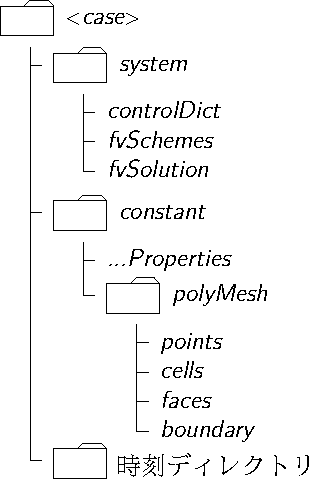
\includegraphics{fig-4-1}
  \hskip10pt
  \begin{minipage}[b]{7zw}
   \def\baselinestretch{1.2}\selectfont
   \autoref{sec:4.3}を参照\par
   \autoref{sec:4.4}を参照\par
   \autoref{sec:4.5}を参照\par
   \vskip28pt
   \autoref{chap:7}を参照\par
   \vskip4pt
   \autoref{ssec:5.1.2}を参照\par
   \vskip81pt
   \autoref{ssec:4.2.8}を参照\par
   \vskip-10pt\null
  \end{minipage}
 \end{minipage}
 \caption{ケースディレクトリの構造}
 \label{fig:4.1}
\end{figure}


\begin{description}
 \item[\OFpath{constant}ディレクトリ]
\index{constant@\OFpath{constant}!ディレクトリ}%
\index{ディレクトリ!constant@\OFpath{constant}}%
            そのケースのメッシュに関する全ての情報を含むサブディレクトリ
\index{polyMesh@\OFpath{polyMesh}!ディレクトリ}%
\index{ディレクトリ!polyMesh@\OFpath{polyMesh}}%
            \OFpath{polyMesh},
            および使おうとしているアプリケーションのための
            物性値を定めるファイル (例えば\OFdictionary{transportProperties}) が
            格納されています.
 \item[\OFpath{system}ディレクトリ]
\index{system@\OFpath{system}!ディレクトリ}%
\index{ディレクトリ!system@\OFpath{system}}%
            解析の手順に関連するパラメータ設定のための
            ディレクトリです.
            少なくとも以下の三つのファイルを含みます.
            パラメータが開始/終了時間や時間ステップ
            およびデータのアウトプットのためのパラメータの設定を行う
\index{controlDict@\OFdictionary{controlDict}!ディクショナリ}%
\index{ディクショナリ!controlDict@\OFdictionary{controlDict}}%
            \OFdictionary{controlDict},
            実行時に選択される解析に使われるスキームを
            記述している
\index{fvSchemes@\OFdictionary{fvSchemes}!ディクショナリ}%
\index{ディクショナリ!fvSchemes@\OFdictionary{fvSchemes}}%
            \OFdictionary{fvSchemes},
            そして実行のために方程式のソルバ,許容誤差およびその他の
            アルゴリズム制御を設定する
\index{fvSolution@\OFdictionary{fvSolution}!ディクショナリ}%
\index{ディクショナリ!fvSolution@\OFdictionary{fvSolution}}%
            \OFdictionary{fvSolution}です.
 \item[時刻ディレクトリ]
            特定のフィールドに関するデータの個別のファイルを含んでいます.
            データは,問題を定義するためにユーザが指定する
            初期値と境界条件,または書き込まれたOpenFOAMのファイルの
            結果が存在します.OpenFOAMのフィールドは,
            定常状態の問題のように厳密に解く必要のない場合であっても,
            常に初期化する必要があることに留意してください.
            各時刻ディレクトリの名称は,
            データが書き込まれた時点のシミュレーションが行われた
            時刻に基づいており,
            詳細については\autoref{sec:4.3}に記述されています.
            私達は通常時間$t = 0$でシミュレーションを始めて,
            初期条件は指定された名前のフォーマットに応じて
\index{0@\OFpath{0}!ディレクトリ}%
\index{ディレクトリ!0@\OFpath{0}}%
            \OFpath{0}または
\index{0.000000e+00@\OFpath{0.000000e+00}!ディレクトリ}%
\index{ディレクトリ!0.000000e+00@\OFpath{0.000000e+00}}%
            \OFpath{0.000000e+00}と名付けられたディレクトリの中に
            通常収納されるため,十分といえます.
            例えば,\OFcase{cavity}のチュートリアルで,
            速度場の$\bm{U}$と圧力場の$p$それぞれファイル
            \OFpath{O/U}と\OFpath{O/p}から初期化されます.
\end{description}



\section{基本的な入出力ファイルのフォーマット}
\label{sec:4.2}
\index{OpenFOAM!ファイルフォーマット}%
\index{ファイルフォーマット}%
OpenFOAMは,文字列,スカラ,ベクトル,テンソル,リスト,
およびフィールド等のデータ構造の範囲を読み込む必要があります.
入出力 (I/O) ファイルのフォーマットはユーザがOpenFOAMの
アプリケーションをできる限り容易に修正できるよう,
非常に柔軟に設計されています.
このI/Oは,ファイルの作成が非常に簡単で理解しやすい
単純なルールに従っているものであり,
ファイルのフォーマットが直観的に理解しづらいばかりか
どこにも公開されていないような,
多くのソフトウェアパッケージとは対照的です.
OpenFOAMのファイルフォーマットについては次節で説明します.


\subsection{一般的な構文規則}
\label{ssec:4.2.1}
フォーマットは以下のC++ソースコードの
いくつかの一般的な原理に従います.
\begin{itemize}
 \item ファイルは,列によって特定の意味が割り当てられることもなく,
       継続行を明示する必要もない,自由形式となっています.
 \item 行は特に意味をもちませんが,
\index{//@\verb+//+!OpenFOAMファイルこうぶん@OpenFOAMファイル構文}%
\index{OpenFOAMファイルこうぶん@OpenFOAMファイル構文!//@\verb+//+}%
       コメント・デリミタ \verb|//| があればOpenFOAMは行の最後までテキストを無視します.
 \item 複数行にわたるコメントは,\verb|/*| と \verb|*/| で囲みます.
\end{itemize}


\subsection{ディクショナリ}
\label{ssec:4.2.2}
OpenFOAMにおいてデータを指定する最も一般的な手段としては\emph{ディクショナリ}を使います.
ディクショナリには,\emph{キーワード}に応じてI/Oから読み出すことのできるデータ項目が含まれています.
キーワード・エントリは以下のような一般的な書式に従います.
\begin{OFverbatim}[file]
<keyword>  <dataEntry1> ... <dataEntryN>;
\end{OFverbatim}
ほとんどの入力項目は単一のデータ入力の書式になっています
\begin{OFverbatim}[file]
<keyword>  <dataEntry>;
\end{OFverbatim}
ほとんどのOpenFOAMのデータファイルはそれ自体1セットの
キーワード入力を含むディクショナリです.
ディクショナリは論理的なカテゴリにエントリを構成するための手段を提供しており,
階層的に指定できるので,
どんなディクショナリもそれ自体が一つ以上のディクショナリエントリを含んでいます.
ディクショナリの書式は,以下のようにディクショナリ名を指定し,
その後に波括弧 \verb|{ }| で囲まれたキーワード・エントリが続きます.
\begin{OFverbatim}[file]
<dictionaryName>
{
    ... keyword entries ...
}
\end{OFverbatim}


\subsection{データファイルヘッダ}
\label{ssec:4.2.3}
OpenFOAMによって読み書きされるすべてのデータファイルは,
\autoref{tbl:4.1}に記載されており,
キーワード入力の標準セットを含む
\index{FoamFile@\OFkeyword{FoamFile}!キーワード}%
\index{キーワード!FoamFile@\OFkeyword{FoamFile}}%
\OFkeyword{FoamFile}と
名付けられたディクショナリから始まります.


\begin{table}[ht]
 %#! platex UserGuideJa
\begin{tabularx}{\textwidth}{lXX}
 キーワード & 説明 & 入力 \\
 \hline
\index{version@\string\OFkeyword{version}!キーワード}%
\index{キーワード!version@\string\OFkeyword{version}}%
 \OFkeyword{version} & 入出力形式のバージョン & 2.0 \\
\index{format@\string\OFkeyword{format}!キーワード}%
\index{キーワード!format@\string\OFkeyword{format}}%
 \OFkeyword{format} & データ形式 & \OFkeyword{ascii} / \OFkeyword{binary} \\
\index{location@\string\OFkeyword{location}!キーワード}%
\index{キーワード!location@\string\OFkeyword{location}}%
 \OFkeyword{location} & ``...''ファイルへのパス & (オプション) \\
\index{class@\string\OFkeyword{class}!キーワード}%
\index{キーワード!class@\string\OFkeyword{class}}%
 \OFkeyword{class} & 関連するデータファイルから構成されたOpenFOAMのクラス &
         一般的に\OFkeyword{dictionary}もしくは領域,\hfil\break
         例:\OFkeyword{volVectorField} \\
\index{object@\string\OFkeyword{object}!キーワード}%
\index{キーワード!object@\string\OFkeyword{object}}%
 \OFkeyword{object} & ファイル名 & 例:\OFpath{controlDict} \\
 \hline
\end{tabularx}

 \caption{データファイルのためのヘッダのキーワード入力}
 \label{tbl:4.1}
\end{table}


この表には各エントリの簡単な説明を載せています.
これは\OFkeyword{class}については多くの例外があるものの,
おそらくほとんどのエントリについては十分な内容でしょう.
\OFkeyword{class}エントリはファイル内のデータから構成される
OpenFOAMライブラリでのC++クラスの名前です.
おそらくユーザは,読み込まれるファイルを呼び出す基礎的なコードの知識や
OpenFOAMクラスの知識なしに,
\OFkeyword{class}の入力を正確に推測することはできません.
しかし,ほとんどのデータファイルは単純なキーワードエントリをもち
内部の\OFclass{dictionary}クラスの中に読み込まれます.
それゆえ,それらの場合では\OFkeyword{class}エントリは\OFkeyword{dictionary}となります.

以下の例はこれまで説明してきたエントリのタイプを使った
ケースへのデータ供給のキーワードの使い方を示しています.
\OFdictionary{fvSolution}ディクショナリファイルを分解すると,
\OFdictionary{solvers}と\OFdictionary{PISO}という二つのディクショナリが含まれています.
\OFdictionary{solvers}ディクショナリは
圧力方程式と速度方程式に対してそれぞれ計算用と収束用に複数のデータ入力があり,
それぞれ\OFkeyword{p}と\OFkeyword{U}のキーワードによって記述されます.
\OFdictionary{PISO}ディクショナリはアルゴリズムの制御パラメータを含みます.
\begin{OFverbatim}[file, linenum=17]

solvers
{
    p
    {
        solver           PCG;
        preconditioner   DIC;
        tolerance        1e-06;
        relTol           0;
    }

    U
    {
        solver           smoothSolver;
        smoother         symGaussSeidel;
        tolerance        1e-05;
        relTol           0;
    }
}

PISO
{
    nCorrectors     2;
    nNonOrthogonalCorrectors 0;
    pRefCell        0;
    pRefValue       0;
}


// ************************************************************************* //
\end{OFverbatim}


\subsection{リスト}
\label{ssec:4.2.4}
OpenFOAMアプリケーションはリストを含んでいます.
例えば,メッシュ記述のための頂点リストがあります.
リストは一般的にI/Oにあり独自のフォーマットをもっていて,
入力は丸括弧 \verb|( )| 内にされます.
また,丸括弧の前のフォーマットの選択もあります.
\begin{description}
 \item[simple]
            キーワードに続いてすぐに丸括弧がくる.
\begin{OFverbatim}[file]
    <listName>
    (
        ... entries ...
    );
\end{OFverbatim}
 \item[numbered]
            キーワードに続いてリスト内の要素数 \verb|<n>| がくる.
\begin{OFverbatim}[file]
    <listName>
    <n>
    (
        ... entries ...
    );
\end{OFverbatim}
 \item[token identifier]
            キーワードに続いてクラス名の識別子ラベル \verb|<Type>| がくる.
            \verb|<Type>| はリストに何が入っているかを記載したもので,
            例えばスカラ要素のリストであれば次のようになる.
\begin{OFverbatim}[file]
    <listName>
    List<scalar>
    <n>        // optional
    (
        ... entries ...
    );
\end{OFverbatim}
\end{description}
ここで留意すべきはリスト \verb|<scalar>| での \verb|<scalar>| は
一般名ではなく入力された実際の文字列です.
単純なフォーマットは,リストを書くときの便利な方法です.
その他のフォーマットはリストのサイズがデータを読み込む前に
メモリに割り当てられるのでコードがより早くデータを読み込めます.
それゆえ単純なフォーマットは読み込み時間が最小の短いリストに適しており,
その他のフォーマットは長いリストに適しています.


\subsection{スカラとベクトル,テンソル}
\label{ssec:4.2.5}
スカラは,データファイルでは一つの数字として記述されます.
\index{vector@\OFclass{vector}!クラス}%
\index{クラス!vector@\OFclass{vector}}%
\OFclass{vector}は,ランク$1$で3\nobreak 次元の\OFemph{VectorSpace}であり,
要素数はいつも$3$に決まっているので単純なリストフォーマットで使われます.
それゆえ,ベクトル$(1.0,\ 1.1,\ 1.2)$は次のように書かれます.
\begin{OFverbatim}[file]
(1.0 1.1 1.2)
\end{OFverbatim}
OpenFOAMでは,テンソルはランク$2$で3\nobreak 次元の\OFemph{VectorSpace}であり,
それゆえデータ入力はいつも九つの実数と決まっています.
それゆえ単位テンソルは以下のように書かれます.
\begin{OFverbatim}[file]
(
    1 0 0
    0 1 0
    0 0 1
)
\end{OFverbatim}
この例は入力が複数の行に上書きできるように
OpenFOAMがその行に戻るのを無視する方法を示しています.
一行に数字を羅列することと扱いは違いません.
\begin{OFverbatim}[file]
( 1 0 0 0 1 0 0 0 1 )
\end{OFverbatim}


\subsection{次元の単位}
\label{ssec:4.2.6}
\index{じげんのたんい@次元の単位}%
連続体力学では,物理量はある決められた単位で表現されます.
例えば,質量ならキログラム ($\unit*{kg}$),体積なら立法メートル ($\unit*{m^{3}}$),
圧力ならパスカル ($\unit*{kg\,m^{-1}\,s^{-2}}$)というように.
代数の演算は統一した
\index{たんい@単位!そくりょう@測量\jdash}%
測量単位を用いて実行されなければなりません.
特に,足し算,引き算,および等式は同じ次元の単位の物理的特性においてのみ
意味があります.無意味な操作を実行することへの安全装置として,
OpenFOAMはフィールドデータと物理的特性に次元を付けて,
どのようなテンソル操作についても次元を
\index{じげん@次元!OpenFOAMにおけるチェック}%
チェックして実行します.
\OFkeyword{dimensionSet}の入出力形式は角括弧内の七つのスカラ量です.
例えば,
\begin{OFverbatim}[file]
[0 2 -1 0 0 0 0]
\end{OFverbatim}

\autoref{tbl:4.2}に記載するように
各値は計測基準単位のそれぞれの物理量に対応しています.
表は
\index{たんい@単位!SI}%
\index{たんい@単位!Syst\`eme International}%
国際単位系 (SI) と
\index{たんい@単位!USCS}%
\index{たんい@単位!United States Customary System}%
\index{USCS!たんい@単位}%
the United States Customary System (USCS) の
\index{たんい@単位!きほん@基本\jdash}%
基本単位ですが
OpenFOAMはどの単位系も使えます.
要求されることは入力データが選択した単位に合っているということです.
特に重要なのは,OpenFOAMがいくつかの次元化された物理定数を必要とする
ということを知っておくことです.
例えば熱力学のモデル化したある計算のための一般気体定数$R$などがいい例です.
これらの次元定数は
OpenFOAMインストール (\OFpath{\$WM\_PROJECT\_DIR/etc/controlDict}) の
メイン\OFdictionary{controlDict}ファイルの
\OFpath{DimensionedConstant}サブディクショナリで指定されます.
デフォルトでは,これらの定数はSIで設定されます.
USCSもしくはその他の単位系を使用したい場合は,
選択した単位系に合わせてこれらの定数を変更してください.


\begin{table}[t]
 %#! platex UserGuideJa
\begin{tabular}{clll}
\index{SIたんい@SI単位}%
 No. & 物理量 & SI単位 & USCS単位 \\
 \hline
 1 & 質量 & キログラム ($\unit*{kg}$) & 質量ポンド ($\unit*{lbm}$) \\
 2 & 長さ & メートル ($\unit*{m}$) & フィート ($\unit*{ft}$) \\
 3 & 時間 & \multicolumn{2}{c}{秒 ($\unit*{s}$)} \\
 4 & 温度 & ケルビン ($\unit*{K}$) & ランキン温度 ($\unit*{\degR}$) \\
 5 & 物質量 & モル ($\unit*{mol}$)\footnotemark & ポンドモル ($\unit*{lbmol}$) \\
 6 & 電流 & \multicolumn{2}{c}{アンペア ($\unit*{A}$)} \\
 7 & 光度 & \multicolumn{2}{c}{カンデラ ($\unit*{cd}$)} \\
 \hline
\end{tabular}

 \caption{SIとUSCSの基本単位}
 \label{tbl:4.2}
\end{table}
\footnotetext{訳注:原文では$\unit*{kgmol}$とされているが,これは誤り.
SIにおける物質量の基本単位は$\unit*{mol}$である.}%


\subsection{次元付きの型}
\label{ssec:4.2.7}
物理量は一般に,それらの関連する次元によって特定されます.
これらの入力は,\break
\OFkeyword{dimensionedScalar}の
以下の例が示すフォーマットをもっています.
\begin{OFverbatim}[file]
nu             nu  [0 2 -1 0 0 0 0]  1;
\end{OFverbatim}
最初の\OFkeyword{nu}はキーワード,2番目の\OFkeyword{nu}はクラスのwordの名前で,
通常キーワードと同じものが選ばれる.
その次の入力は\OFemph{dimensionSet}で最終的な入力はスカラ値です.


\subsection{フィールド}
\label{ssec:4.2.8}
OpenFOAMの入出力データの多くはテンソル場,
例えば速度や圧力のデータにあり,
時刻ディレクトリから読み込み時刻ディレクトリに書き込まれます.
\autoref{tbl:4.3}で説明されるように,
キーワード入力を使って,OpenFOAMはフィールドデータを書きこみます.


\begin{table}[ht]
 %#! platex UserGuideJa
\begin{tabular}{lll}
 キーワード & 説明 & 例 \\
 \hline
 \tblstrut
\index{dimensions@\OFkeyword{dimensions}!キーワード}%
\index{キーワード!dimensions@\OFkeyword{dimensions}}%
 \OFkeyword{dimensions} & 領域の次元 & \texttt{[1 1 -2 0 0 0 0]} \\
\index{internalField@\OFkeyword{internalField}!キーワード}%
\index{キーワード!internalField@\OFkeyword{internalField}}%
 \OFkeyword{internalField} & 内部領域の値 & \texttt{uniform (1 0 0)} \\
\index{boundaryField@\OFkeyword{boundaryField}!キーワード}%
\index{キーワード!boundaryField@\OFkeyword{boundaryField}}%
 \OFkeyword{boundaryField} & 境界領域 & \autoref{ssec:4.2.8}のファイル参照 \\
 \hline
\end{tabular}

 \caption{フィールドディクショナリで使われる主なキーワード}
 \label{tbl:4.3}
\end{table}


データは\OFkeyword{dimensions}エントリから始まります.
その後に続くのは,以下のいずれかの方法で記述される\OFkeyword{internalField}です.
\begin{description}
 \item[一様フィールド]
            ただひとつの値にそのフィールド内で全ての要素が対応していて,
            以下のような書式をとります.
\begin{OFverbatim}[file]
internalField uniform <entry>;
\end{OFverbatim}
 \item[非一様フィールド]
            各フィールドの要素は,固有の値を割り当てられ,
            リストの識別子トークンフォームにある
            以下の書式をとることが推奨されます.
\begin{OFverbatim}[file]
internalField nonuniform <List>;
\end{OFverbatim}
\end{description}
\OFpath{boundaryField}は\OFpath{polyMesh}ディレクトリ内の
\OFpath{boundary}ファイルにある境界パッチの
それぞれの名前に対応する名前の一連の入力を含んだディクショナリである.
各パッチの入力はそれ自体がキーワード入力のリストを含むディクショナリとなります.
必須エントリである\OFkeyword{type}には,
そのフィールドに指定すべきパッチ・フィールド条件を記述します.
残りの入力は選択されたパッチ・フィールド条件のタイプに対応し,
一般的にはパッチフェイスで初期条件を分類するフィールドデータを含みます.
OpenFOAMで使えるパッチ・フィールド条件の選択肢は,
その説明と指定しなければならないデータと併せて,
\autoref{tbl:5.3}と\autoref{tbl:5.4}に記載してあります.
速度\OFkeyword{U}のフィールドのディクショナリ入力の例を以下に示します.
\begin{OFverbatim}[file, linenum=17]
dimensions      [0 1 -1 0 0 0 0];

internalField   uniform (0 0 0);

boundaryField
{
    movingWall
    {
        type            fixedValue;
        value           uniform (1 0 0);
    }

    fixedWalls
    {
        type            fixedValue;
        value           uniform (0 0 0);
    }

    frontAndBack
    {
        type            empty;
    }
}

// ************************************************************************* //
\end{OFverbatim}


\subsection{ディレクティブとマクロ置換}
\label{ssec:4.2.9}
OpenFOAMのケースファイルを柔軟に設定するためのディレクティブや
代替マクロといったオプションのファイル構文があります.
ディレクティブはケースファイル内で \verb|#| から始まるコマンドとして記述されます.
代替マクロは \verb|$| から始まります.%$

OpenFOAMでは現在$4$種類のディレクティブが利用可能できます.
\begin{description}
 \item[\texttt{\char'043include "<fileName>"}]
            または \texttt{\char'043includeIfPresent "<fileName>"}
            \OFpath{<fileName>}という名前のファイルを読み込む
 \item[\texttt{\char'043inputMode}]
            二つのオプションがある.
            \OFkeyword{merge}は連続するディクショナリのキーワードのエントリを統合する.
            つまりある場所で指定されたキーワードのエントリを継承して
            以後の同一キーワードのエントリが指定される.
            \OFkeyword{overwrite}はディクショナリ全体を上書きする.
            通常は\OFkeyword{merge}を使う.
 \item[\texttt{\char'043remove <keywordEntry>}]
            インクルードされた全てのキーワードエントリを削除する.
            単語または正規表現で指定できる.
 \item[\texttt{\char'043codeStream}]
            続けてC++ソースコードを書くと,
            そのコードを即席でコンパイル・ロード・実行し,エントリを生成する.
\end{description}


\subsection{\texttt{\char'043include}および\hskip\xkanjiskip\texttt{\char'043inputMode}ディレクティブ}
\label{ssec:4.2.10@2.0.0}
一度使われた圧力の初期値を,内部フィールドと境界の初期値に設定する例を示します.
以下の記述を含む\OFpath{initialConditions}というファイルを作成していたとします.
\begin{OFverbatim}[file]
pressure 1e+05;
#inputMode merge
\end{OFverbatim}
この圧力をフィールド内部と境界に用いるために,
以下の代替マクロを圧力場のファイル\OFpath{p}に記述します.
\begin{OFverbatim}[file]
#include "initialConditions"
internalField uniform $pressure;
boundaryField
{
    patch1
    {
        type fixedValue;
        value $internalField;
    }
}
\end{OFverbatim}
あくまでもこれは,この機能がどのように働くかを示しただけの単純な例です.
しかしこの機能は,ケースデータをユーザのニーズに合わせて一般化する手段として,
より便利な使い方で多く用いることができます.
例えば同一のRAS乱流モデルの設定を用いるケースがいくつかある場合,
その設定を記述したファイルを一つ作成し,
各ケースの\OFpath{RSAProperties}ファイルに\texttt{include}によって
組み込めばよいのです.代替マクロは単独の値にとどまりません.
例えば,単独のマクロで境界条件のまとまりを事前に定義して,それをよびだすことができます.
この機能はほぼどこでも使えます.


\subsection{\texttt{\char'043codeStream}ディレクティブ}
\label{ssec:4.2.11@2.0.0}
\verb|#codeStream|ディレクティブはC++コードをコンパイル・実行して,
ディクショナリのエントリを生成します.
コードとコンパイル方法は以下のキーワードで指定します.
\begin{itemize}
 \item \texttt{code}: コードを指定します.
       これは\verb|OStream& os|および\verb|dictionary& dict|を引数とし,
       ユーザはコードの中でこれらの引数を使うことができます.
       例えば,当該ケースのディクショナリ(ファイル)から
       キーワード・エントリを取り出すことができます.
 \item \texttt{codeInclude}(オプション): OpenFOAMファイルを読み込むため,
       追加のC++ \verb|#include|文を指定できます.
 \item \texttt{codeOptions}(オプション): \OFpath{Make/options}の中の
       \verb|EXE_INC|に加えて,追加のコンパイル・フラグを指定できます.
 \item \texttt{codeLibs}(オプション): \OFpath{Make/options}の中の
       \verb|LIB_LIBS|に加えて,追加のコンパイル・フラグを指定できます.
\end{itemize}
コードは,ハッシュ・ブラケット記号,
すなわち\hskip\xkanjiskip\verb|#{...#}|\hskip\xkanjiskip で囲むことで,
通常の文字列と同じように複数行にわたって書くことができます.
この二つの記号の間のあらゆるものは,全ての改行・引用符などの予約語とともに,
一つの文字列となります.

以下に\hskip\xkanjiskip\verb|#codeStream|の例を示します.
このコードは\OFpath{controlDict}ファイル内に書かれており,
ディクショナリ・エントリを取り出し,出力間隔を決めるための簡単な計算を施しています.
\begin{OFverbatim}[file]
startTime       0;
endTime         100;
...
writeInterval   #codeStream
{
    code
    #{
        scalar start = readScalar(dict.lookup("startTime"));
        scalar end = readScalar(dict.lookup("endTime"));
        label nDumps = 5;
        os << ((end - start)/nDumps);
    #};
};
\end{OFverbatim}



\section{時間とデータの入出力制御}
\label{sec:4.3}
\index{じかんの@時間の!せいぎょ@制御}%
\index{せいぎょ@制御!じかんの@時間の\jdash}%
OpenFOAMのソルバは全て,
データベースをセットアップすることによって,動き始めます.
データベースは入出力を制御し,またデータの出力は通常実行中,
時間ごとに要求されるので,時間はデータベースにとって不可避の要素です.
\OFdictionary{controlDict}ディクショナリはデータベースの作成に不可欠な
入力パラメータを設定します.
\OFdictionary{controlDict}のキーワード入力項目は
\autoref{tbl:4.4}に記載されています.
時間制御方式と\OFkeyword{writeInterval}入力だけは完全に強制的で,
省略できる任意の項目には\autoref{tbl:4.4}で示された
デフォルト値のデータベースが用いられます.


\vskip\floatsep
\begingroup
 \small
% \begin{table}[ht]
 \LTXtable{\textwidth}{tbl/tbl-4-4}
 \addtocounter{table}{-1}%
 \tblcaption{controlDictディクショナリのキーワード項目}
 \label{tbl:4.4}
% \end{table}
\endgroup
\vskip\floatsep


以下に\OFdictionary{controlDict}ディクショナリの入力例を示します.
\begin{OFverbatim}[file, linenum=17]

application     icoFoam;

startFrom       startTime;

startTime       0;

stopAt          endTime;

endTime         0.5;

deltaT          0.005;

writeControl    timeStep;

writeInterval   20;

purgeWrite      0;

writeFormat     ascii;

writePrecision  6;

writeCompression off;

timeFormat      general;

timePrecision   6;

runTimeModifiable true;


// ************************************************************************* //
\end{OFverbatim}



\section{数値スキーム}
\label{sec:4.4}
\OFpath{system}ディレクトリにある
\index{fvSchemes@\OFdictionary{fvSchemes}!ディクショナリ}%
\index{ディクショナリ!fvSchemes@\OFdictionary{fvSchemes}}%
\OFdictionary{fvSchemes}ディクショナリは,
アプリケーションの実行時に現われる,
方程式における導関数等の項に対する数値スキームを設定します.
この節では,\OFdictionary{fvSchemes}ディクショナリにおいてどのように,
これらのスキームを指定するかを説明します.

\OFdictionary{fvSchemes}において数値スキームを割りあてなければならない典型的な項は,
例えば空間勾配といった導関数項や,
一つの点集合から他の集合へと値を補間する項等です.
OpenFOAMでは,ユーザに制限無くスキームを選択できるようにしたいと思っています.
例えば,線形補間は多くのケースで効率的ですが,
OpenFOAMでは,全ての補間項に対して幅広い補間スキームの中から
自由に選択ができるようになっています.

導関数の項は,このような選択の自由のさらなる好例となります.
ユーザは,まず離散化手法を選択することができますが,
ここではGaussによる有限体積積分を用いるのが一般的です.
Gauss積分は格子の界面における値を足していくことで実現されますが,
界面での値は格子中心での値から補間しなければなりません.
この補間スキームにおいてもユーザは自由に選ぶことができ,
特定の導関数項,特に対流項に用いる発散項には,
特別に設計されたいくつかのスキームが用意されています.
数値スキームを指定しなければならない項はいろいろありますが,
それらは\OFdictionary{fvSchemes}ディクショナリにおいて
\autoref{tbl:4.5}に示すカテゴリに分類されます.
\autoref{tbl:4.5}における各キーワードはサブディクショナリの名前ですが,
それらは各々特定のタイプの項を持っているわけです.
例えば,\OFkeyword{gradSchemes}には\OFkeyword{grad(p)}(と表現される)といった
全ての勾配項があります.
その他の例は,以下に示した
\index{fvSchemes@\OFdictionary{fvSchemes}!ディクショナリ}%
\index{ディクショナリ!fvSchemes@\OFdictionary{fvSchemes}}%
\OFdictionary{fvSchemes}ディクショナリの抜粋をご覧ください.


\begin{table}[ht]
 %#! platex UserGuideJa
\begin{tabular}{ll}
 キーワード & 数学的タームのカテゴリ \\
 \hline
\index{interpolationSchemes@\OFkeyword{interpolationSchemes}!キーワード}%
\index{キーワード!interpolationSchemes@\OFkeyword{interpolationSchemes}}%
 \OFkeyword{interpolationSchemes} & 2点間の値の補間 \\
\index{snGradSchemes@\OFkeyword{snGradSchemes}!キーワード}%
\index{キーワード!snGradSchemes@\OFkeyword{snGradSchemes}}%
 \OFkeyword{snGradSchemes} & 格子界面の法線方向勾配の各要素 \\
\index{gradSchemes@\OFkeyword{gradSchemes}!キーワード}%
\index{キーワード!gradSchemes@\OFkeyword{gradSchemes}}%
 \OFkeyword{gradSchemes} & 勾配$\nabla$ \\
\index{divSchemes@\OFkeyword{divSchemes}!キーワード}%
\index{キーワード!divSchemes@\OFkeyword{divSchemes}}%
 \OFkeyword{divSchemes} & 発散$\nabla \cdot {}$ \\
\index{laplacianSchemes@\OFkeyword{laplacianSchemes}!キーワード}%
\index{キーワード!laplacianSchemes@\OFkeyword{laplacianSchemes}}%
 \OFkeyword{laplacianSchemes} & Laplacian $\Laplacian$ \\
\index{timeScheme@\OFkeyword{timeScheme}!キーワード}%
\index{キーワード!timeScheme@\OFkeyword{timeScheme}}%
 \OFkeyword{timeScheme} & 1次と2次の時間導関数$\partial/\partial t$,$\partial^{2}/\partial^{2}t$ \\
\index{fluxRequired@\OFkeyword{fluxRequired}!キーワード}%
\index{キーワード!fluxRequired@\OFkeyword{fluxRequired}}%
 \OFkeyword{fluxRequired} & フラックスの生成が必要な物理量 \\
 \hline
\end{tabular}

 \caption{fvSchemesで使用する主なキーワード}
 \label{tbl:4.5}
\end{table}


\begin{OFverbatim}[file, linenum=17]

ddtSchemes
{
    default         Euler;
}

gradSchemes
{
    default         Gauss linear;
    grad(p)         Gauss linear;
}

divSchemes
{
    default         none;
    div(phi,U)      Gauss linear;
}

laplacianSchemes
{
    default         Gauss linear orthogonal;
}

interpolationSchemes
{
    default         linear;
}

snGradSchemes
{
    default         orthogonal;
}

fluxRequired
{
    default         no;
    p               ;
}


// ************************************************************************* //
\end{OFverbatim}
この例を見ると\OFdictionary{fvSchemes}ディクショナリは
以下の要素から成り立っていることがわかります.
\begin{itemize}
 \item 六つの\OFsubdictionary{...Schemes}のサブディクショナリには,
       指定した各項に対するキーワードが書いてあり,
       \OFkeyword{default}のキーワードも指定できますが,
       その他にも,例えば$\nabla p$については\OFkeyword{grad(p)}というように,
       特定の項に対して名前を書くことで,
       それに対応するキーワードを指定することができます.
 \item \OFsubdictionary{fluxRequired}のサブディクショナリには,
       例えば\OFkeyword{p}のように,
       アプリケーションの中でフラックスが生成される場が書かれています.
\end{itemize}
もし,\OFkeyword{default}のスキームが
特定の\OFsubdictionary{...Schemes}のサブディクショナリで指定された場合には,
サブディクショナリが参照している全ての項にそのスキームが適用されます.
例えば,\OFsubdictionary{gradSchemes}において
\OFkeyword{default}が指定されている場合には,そのアプリケーションにおける,
$\nabla p$,$\nabla\bm{U}$といった全ての勾配項に対して,
その\OFkeyword{default}のスキームが適用されるわけです.
\OFkeyword{default}が指定されているときには,
そのサブディクショナリにおいて各項のスキームをいちいち指定する必要がなくなります.
この例では,\OFkeyword{grad(p)},\OFkeyword{grad(U)}の行がそれです.
しかしながら,特定の項の行が挿入された場合,
その項に対しては,指定されたスキームが\OFkeyword{default}より優先されます.

かわりに,ユーザは
\index{none@\OFkeyword{none}!キーワードエントリ}%
\index{キーワードエントリ!none@\OFkeyword{none}}%
\OFkeyword{none}エントリにより,
あえて\OFkeyword{default}スキームを使わないようにもできます.
この場合には,ユーザはそのサブディクショナリの中の全ての項を
個々に指定しなければなりません.
\OFkeyword{default}は上書きすることができるのですから,
\OFkeyword{default}に\OFkeyword{none}を設定することはやりすぎかもしれません.
しかしながら,\OFkeyword{none}を指定することは,
ユーザが全ての項を個別に指定しなければならないことから,
そのアプリケーションに実際にどの項が存在するかを認識するという点では有用です.

次の節では,\autoref{tbl:4.5}に示した
それぞれのカテゴリの項について,選択できるスキームを述べます.


\subsection{補間スキーム}
\label{ssec:4.4.1}
\OFsubdictionary{interpolationSchemes}サブディクショナリには,
通常,セル中心から界面中心へ値を内挿する項があります.
OpenFOAMでの内挿スキームの選択肢を
\autoref{tbl:4.6}に示しますが,
これは四つのカテゴリに分けられます.
一つのカテゴリは一般的なスキームが,そして他の三つのカテゴリは,
\autoref{ssec:4.4.5}で説明するように,
主に流体での対流(発散)項のGaussの離散化と一緒に使われるものです.
ユーザが\OFsubdictionary{interpolationSchemes}サブディクショナリにおいて,
対流特有のスキームを一般的なフィールドの内挿に適用することは,
「ほとんどない」のですが,有効な内挿スキームとして
\autoref{ssec:4.4.5}よりもむしろここで説明しておきます.
なお,
\index{UMIST@\OFkeyword{UMIST}!キーワードエントリ}%
\index{キーワードエントリ!UMIST@\OFkeyword{UMIST}}%
\OFkeyword{UMIST}のようなスキームもOpenFOAMでは
利用可能なことに注意すべきですが,
一般的に推奨されるスキームのみを\autoref{tbl:4.6}に示します.

普通のスキームは,単にキーワードとエントリのみを記すことで指定でき,
例えば\OFkeyword{linear}スキームを\OFkeyword{default}として指定するには
以下のようにします.
\begin{OFverbatim}[file]
default linear;
\end{OFverbatim}
対流特有のスキームは,流れの速度による流束に基づいて内挿を行います.
これらのスキームを指定する場合には,
内挿のベースとなる流束場の名前が必要ですが,
ほとんどのOpenFOAMのアプリケーションでは,
これは\OFkeyword{phi}となっており,この名前は,通常,
\OFkeyword{surfaceScalarField}の速度の流束に対応するものです.
このガイドの中では,対流特有のスキームの三つのカテゴリは,
general convection,normalised variable (NV),
そして,total variation diminishing (TVD) と記述されます.
\OFkeyword{blended}スキームを除いて,
general convectionとTVDスキームは,
そのスキーム名と流束場によって指定され,
例えば流束\OFkeyword{phi}に基づく\OFkeyword{upwind}スキームを
\OFkeyword{default}として指定するには以下のようにします.
\begin{OFverbatim}[file]
default upwind phi;
\end{OFverbatim}
いくつかのTVD/NVDスキームには,$0 \le \psi \le 1$の範囲の係数$\psi$が必要ですが,
$\psi = 1$はTVD条件に従うことに対応し,通常最も良い収束性を示すのに対し,
$\psi = 0$は最も良い精度を与えます.通常$\psi = 1$での実行がお勧めです.
流束\OFkeyword{phi}に基づく$\psi = 1.0$での\OFkeyword{limitedLinear}スキームを,
\OFkeyword{default}として指定するには以下のようにします.
\begin{OFverbatim}[file]
default limitedLinear 1.0 phi;
\end{OFverbatim}

\subsubsection{厳密に範囲が限定されるスカラ量に対するスキーム}
\label{sssec:4.4.1.1}
厳密に範囲が限定される必要のあるスカラ量のために,
いくつかの制限付きスキームという拡張版があります.
ユーザが指定した範囲に限定するためには,
スキームの名前には\OFkeyword{limited}という語が頭に付けられ,
下限と上限それぞれを続けて指定します.
例えば,\OFkeyword{vanLeer}スキームを$-2$と$3$の間で
厳密に制限するためには,次のように指定します.
\begin{OFverbatim}[file]
default limitedVanLeer -2.0 3.0;
\end{OFverbatim}
よく使われる$0$と$1$の間で限定されるスカラ場のために
特化された版もあります.
それらは,スキームの名前に\OFkeyword{01}を付けることで選択できます.
例えば,\OFkeyword{vanLeer}スキームを$0$と$1$の間で
厳密に限定するためには,以下のように指定します.
\begin{OFverbatim}[file]
default vanLeer01;
\end{OFverbatim}
厳密に範囲が限定する拡張版は,
\OFkeyword{limitedLinear},\OFkeyword{vanLeer},\OFkeyword{Gamma},
\OFkeyword{limitedCubic},\OFkeyword{MUSCL},\OFkeyword{SuperBee}の
スキームで利用することができます.

\subsubsection{ベクトル場に対するスキーム}
\label{sssec:4.4.1.2}
ベクトル場に対する制限付きスキームについては,
場の方向を考慮にいれて構成された改良版のリミッタがあります.
これらのスキームは,通常のスキームの名前に\OFkeyword{V}を
加えることで選択することができ,
\OFkeyword{limitedLinear}に対しては\OFkeyword{limitedLinearV}といった具合です.
これら\OFkeyword{V}版は\OFkeyword{limitedLinearV},\OFkeyword{vanLeerV},
\OFkeyword{GammaV},\OFkeyword{limitedCubicV},\OFkeyword{SFCDV}といったスキームで
利用することができます.


\begin{table}[ht]
 %#! platex UserGuideJa
\begin{tabular}{ll}
 \multicolumn{2}{l}{中心スキーム} \\
 \hline
 \tblstrut
\index{linear@\OFkeyword{linear}!キーワードエントリ}%
\index{キーワードエントリ!linear@\OFkeyword{linear}}%
 \OFkeyword{linear} & 線形補間(中心差分) \\
\index{cubicCorrection@\OFkeyword{cubicCorrection}!キーワードエントリ}%
\index{キーワードエントリ!cubicCorrection@\OFkeyword{cubicCorrection}}%
 \OFkeyword{cubicCorrection} & キュービックスキーム \\
\index{midPoint@\OFkeyword{midPoint}!キーワードエントリ}%
\index{キーワードエントリ!midPoint@\OFkeyword{midPoint}}%
 \OFkeyword{midPoint} & 均等重み付け線形補間 \\
 \\
 \multicolumn{2}{l}{風上対流スキーム} \\
 \hline
 \tblstrut
\index{upwind@\OFkeyword{upwind}!キーワードエントリ}%
\index{キーワードエントリ!upwind@\OFkeyword{upwind}}%
 \OFkeyword{upwind} & 風上差分 \\
\index{linearUpwind@\OFkeyword{linearUpwind}!キーワードエントリ}%
\index{キーワードエントリ!linearUpwind@\OFkeyword{linearUpwind}}%
 \OFkeyword{linearUpwind} & 線形風上差分 \\
\index{skewLinear@\OFkeyword{skewLinear}!キーワードエントリ}%
\index{キーワードエントリ!skewLinear@\OFkeyword{skewLinear}}%
 \OFkeyword{skewLinear} & ひずみ補正付き線形スキーム \\
\index{filteredLinear2@\OFkeyword{filteredLinear2}!キーワードエントリ}%
\index{キーワードエントリ!filteredLinear2@\OFkeyword{filteredLinear2}}%
 \OFkeyword{filteredLinear2} & 高周波の雑音のフィルタリングを伴う線形スキーム \\
 \\
 \multicolumn{2}{l}{TVDスキーム} \\
 \hline
 \tblstrut
\index{limitedLinear@\OFkeyword{limitedLinear}!キーワードエントリ}%
\index{キーワードエントリ!limitedLinear@\OFkeyword{limitedLinear}}%
 \OFkeyword{limitedLinear} & 有限線形差分 \\
\index{vanLeer@\OFkeyword{vanLeer}!キーワードエントリ}%
\index{キーワードエントリ!vanLeer@\OFkeyword{vanLeer}}%
 \OFkeyword{vanLeer} & van Leerリミッタ \\
\index{MUSCL@\OFkeyword{MUSCL}!キーワードエントリ}%
\index{キーワードエントリ!MUSCL@\OFkeyword{MUSCL}}%
 \OFkeyword{MUSCL} & MUSCLリミッタ \\
\index{limitedCubic@\OFkeyword{limitedCubic}!キーワードエントリ}%
\index{キーワードエントリ!limitedCubic@\OFkeyword{limitedCubic}}%
 \OFkeyword{limitedCubic} & キュービックリミッタ \\
 \\
 \multicolumn{2}{l}{NVDスキーム} \\
 \hline
 \tblstrut
\index{SFCD@\OFkeyword{SFCD}!キーワードエントリ}%
\index{キーワードエントリ!SFCD@\OFkeyword{SFCD}}%
 \OFkeyword{SFCD} & 自動フィルタ中心差分 \\
\index{Gamma@\OFkeyword{Gamma}!キーワードエントリ}%
\index{キーワードエントリ!Gamma@\OFkeyword{Gamma}}%
 \OFkeyword{Gamma} $\psi$ & ガンマ差分 \\
 \hline
\end{tabular}

 \caption{補間スキーム}
 \label{tbl:4.6}
\end{table}


\subsection{表面法線方向勾配スキーム}
\label{ssec:4.4.2}
\OFsubdictionary{snGradSchemes}サブディクショナリは,
表面法線方向勾配の項によるものです.
表面法線方向勾配は,格子の界面で計算されますが,
それは,界面が接続している二つの格子の中心における値の勾配の,
界面の法線方向の成分です.
表面法線方向勾配は,それ自体を使うためにも指定されますが,
Gauss積分を使ってLaplacianを評価する際にも必要となります.

利用可能なスキームを\autoref{tbl:4.7}に示しますが,
これらは単にキーワードとエントリを記述することで指定できます.
ただ,\OFkeyword{limited}は例外で,$0 \le \psi \le 1$の範囲の係数$\psi$を必要とします.
ここで,
\begin{align}
 \label{eq:4.1}
 \psi =
 \begin{cases}
  0 & \text{\OFkeyword{uncorrected}に対応}, \\
  0.333 & \text{非直交補正} \le 0.5 \times \text{直交部分}, \\
  0.5 & \text{非直交補正} \le \text{直交部分}, \\
  1.0 & \text{\OFkeyword{corrected}に対応}.
 \end{cases}
\end{align}
です.

よって,$\psi = 0.5$の\OFkeyword{limited}スキームを
\OFkeyword{default}として指定するには次のようにします.
\begin{OFverbatim}[file]
default limited 0.5;
\end{OFverbatim}


\begin{table}[ht]
 %#! platex UserGuideJa
\begin{tabular}{ll}
 スキーム & 説明 \\
 \hline
 \tblstrut
\index{corrected@\OFkeyword{corrected}!キーワードエントリ}%
\index{キーワードエントリ!corrected@\OFkeyword{corrected}}%
 \OFkeyword{corrected} & 陽的非直交補正 \\
\index{uncorrected@\OFkeyword{uncorrected}!キーワードエントリ}%
\index{キーワードエントリ!uncorrected@\OFkeyword{uncorrected}}%
 \OFkeyword{uncorrected} & 非直交補正なし \\
\index{limited@\OFkeyword{limited}!キーワードエントリ}%
\index{キーワードエントリ!limited@\OFkeyword{limited}}%
 \OFkeyword{limited} $\psi$ & 有限非直交補正 \\
\index{bounded@\OFkeyword{bounded}!キーワードエントリ}%
\index{キーワードエントリ!bounded@\OFkeyword{bounded}}%
 \OFkeyword{bounded} & ポジティブスカラの有界補正 \\
\index{fourth@\OFkeyword{fourth}!キーワードエントリ}%
\index{キーワードエントリ!fourth@\OFkeyword{fourth}}%
 \OFkeyword{fourth} & 4次 \\
 \hline
\end{tabular}

 \caption{表面法線方向勾配スキーム}
 \label{tbl:4.7}
\end{table}


\subsection{勾配スキーム}
\label{ssec:4.4.3}
\OFsubdictionary{gradSchemes}サブディクショナリには勾配項を記述します.
各項の離散化スキームは,\autoref{tbl:4.8}の中から
選択することができます.


\begin{table}[ht]
 %#! platex UserGuideJa
\begin{tabular}{ll}
 離散化スキーム & 説明 \\
 \hline
\index{Gauss@\OFkeyword{Gauss}!キーワードエントリ}%
\index{キーワードエントリ!Gauss@\OFkeyword{Gauss}}%
 \OFkeyword{Gauss} & 1次のガウス積分 \\
\index{leastSquares@\OFkeyword{leastSquares}!キーワードエントリ}%
\index{キーワードエントリ!leastSquares@\OFkeyword{leastSquares}}%
 \OFkeyword{leastSquares} & 2次の最小二乗法 \\
\index{fourth@\OFkeyword{fourth}!キーワードエントリ}%
\index{キーワードエントリ!fourth@\OFkeyword{fourth}}%
 \OFkeyword{fourth} & 4次の最小二乗法 \\
\index{limited@\OFkeyword{limited}!キーワードエントリ}%
\index{キーワードエントリ!limited@\OFkeyword{limited}}%
 \OFkeyword{limited} & 上記のスキームの制限バージョン \\
 \hline
\end{tabular}
 \caption{\OFsubdictionary{gradSchemes}において使用できる離散化スキーム}
 \label{tbl:4.8}
\end{table}


\OFkeyword{leastSquares}と\OFkeyword{fourth}の場合には,
離散化スキームの指定は次のように
そのスキーム名を指定するだけで十分です.
\begin{OFverbatim}[file]
grad(p) leastSqueares;
\end{OFverbatim}
\OFkeyword{Gauss}キーワードは,
Gauss積分による標準的な有限体積法の離散化を指定するもので,
これは,格子の中心から界面の中心への値の内挿を必要とします.
このため,\OFkeyword{Gauss}エントリでは,
\autoref{tbl:4.6}のような内挿スキームを続けて指定する必要があります.
一般的な内挿スキーム以外を選択することはほとんどなく,
ほとんどのケースでは次のように\OFkeyword{linear}スキームを選ぶのが効率的です.
\begin{OFverbatim}[file]
grad(p) Gauss linear;
\end{OFverbatim}
三つの基本的な勾配スキーム (\OFkeyword{Gauss},\OFkeyword{leastSquares},
\OFkeyword{fourth}) の範囲限定版は,
離散化スキームの前に
\OFkeyword{cellLimited} (または\OFkeyword{faceLimited}) を付けることで選択できます.
例えば,セルで制限されたGaussスキームは以下のようになります.
\begin{OFverbatim}[file]
grad(p) cellLimited Gauss linear 1;
\end{OFverbatim}


\subsection{Laplacianスキーム}
\label{ssec:4.4.4}
\OFsubdictionary{laplacianSchemes}サブディクショナリにはLaplacian項を記述します.
流体力学の中で見られる$\nabla \cdot (\rho\nabla\bm{U})$といった典型的なLaplacian項を
どのようにエントリに記述するかというと,
\OFkeyword{laplacian(nu, U)}といったword識別子で与えます.
離散化手法として選べるのは\OFkeyword{Gauss}スキームだけですが,
さらに拡散係数(この例では$\nu$)の内挿スキームや,
$\nabla\bm{U}$に対する表面法線方向勾配スキームの両方を選択する必要があります.
つまり,このエントリは以下のようになります.
\begin{OFverbatim}[file]
Gauss <interpolationScheme> <snGradScheme>
\end{OFverbatim}
内挿スキームは\autoref{tbl:4.6}から選択しますが,
通常は一般的なスキームから選択され,
ほとんどの場合\OFkeyword{linear}にします.
表面法線方向勾配スキームは\autoref{tbl:4.7}から選択し,
\autoref{tbl:4.9}に書かれているように
スキームの選択は数値的性質を決定します.
先の例でのLaplacian項の典型的なエントリは以下のようになります.
\begin{OFverbatim}[file]
laplacian(nu, U) Gauss linear corrected;
\end{OFverbatim}


\begin{table}[ht]
 %#! platex UserGuideJa
\begin{tabular}{ll}
 スキーム & 数値的性質 \\
 \hline
 \tblstrut
\index{corrected@\OFkeyword{corrected}!キーワードエントリ}%
\index{キーワードエントリ!corrected@\OFkeyword{corrected}}%
 \OFkeyword{corrected} & 無制限,2次,保存性 \\
\index{uncorrected@\OFkeyword{uncorrected}!キーワードエントリ}%
\index{キーワードエントリ!uncorrected@\OFkeyword{uncorrected}}%
 \OFkeyword{uncorrected} & 制限,1次,非保存性 \\
\index{limited@\OFkeyword{limited}!キーワードエントリ}%
\index{キーワードエントリ!limited@\OFkeyword{limited}}%
 \OFkeyword{limited} $\psi$ &
 \OFkeyword{corrected}と\OFkeyword{uncorrected}の混合 \\
\index{bounded@\OFkeyword{bounded}!キーワードエントリ}%
\index{キーワードエントリ!bounded@\OFkeyword{bounded}}%
 \OFkeyword{bounded} & 制限スカラの1次 \\
\index{fourth@\OFkeyword{fourth}!キーワードエントリ}%
\index{キーワードエントリ!fourth@\OFkeyword{fourth}}%
 \OFkeyword{fourth} & 無制限,4次,保存性 \\
 \hline
\end{tabular}
 \caption{\OFsubdictionary{laplacianSchemes}における表面法線方向スキームの性質}
 \label{tbl:4.9}
\end{table}


\subsection{発散スキーム}
\label{ssec:4.4.5}
\OFsubdictionary{divSchemes}サブディクショナリには発散項を記述します.
流体力学の中で見られる典型的な対流項$\nabla \cdot (\rho\bm{U}\bm{U})$はどうように記述するかというと,
OpenFOAMのアプリケーションでは通常\OFkeyword{div(phi, U)}という
識別子で与えます.ここで\OFkeyword{phi}はフラックス$\phi = \rho\bm{U}$です.

離散化手法として選べるのは\OFkeyword{Gauss}スキームだけですが,
さらに対象の場(この例では$\bm{U}$)の内挿スキームを選択する必要があります.
つまり,このエントリは以下のようになります.
\begin{OFverbatim}[file]
Gauss <interpolationScheme>
\end{OFverbatim}
内挿スキームは,一般的なものや対流特有のものも含め,
\autoref{tbl:4.6}の中から選択します.
この選択は,\autoref{tbl:4.10}に示すように,数値的性質を大きく決定づけます.
対流特有の内挿スキームを指定する場合でも,
流束は特定の項として既に値がわかっているものとし,
流束の内挿スキームは記述しません.
つまり,例えば\OFkeyword{div(phi, U)}の場合では,
流束は\OFkeyword{phi}として既知ですので,
さらにその内挿スキームを指定すると矛盾が生じるだけです.
よって,先の例での風上型内挿スキームの指定は次のようになります.
\begin{OFverbatim}[file]
div(phi, U) Gauss upwind;
\end{OFverbatim}


\begin{table}[ht]
 %#! platex UserGuideJa
\begin{tabular}{ll}
 スキーム & 数値的性質 \\
 \hline
\index{linear@\OFkeyword{linear}!キーワードエントリ}%
\index{キーワードエントリ!linear@\OFkeyword{linear}}%
 \OFkeyword{linear} & 2次,無制限 \\
\index{skewLinear@\OFkeyword{skewLinear}!キーワードエントリ}%
\index{キーワードエントリ!skewLinear@\OFkeyword{skewLinear}}%
 \OFkeyword{skewLinear} & 2次,(より) 無制限,ひずみ補正 \\
\index{cubicCorrected@\OFkeyword{cubicCorrected}!キーワードエントリ}%
\index{キーワードエントリ!cubicCorrected@\OFkeyword{cubicCorrected}}%
 \OFkeyword{cubicCorrected} & 4次,無制限 \\
\index{upwind@\OFkeyword{upwind}!キーワードエントリ}%
\index{キーワードエントリ!upwind@\OFkeyword{upwind}}%
 \OFkeyword{upwind} & 1次,制限 \\
\index{linearUpwind@\OFkeyword{linearUpwind}!キーワードエントリ}%
\index{キーワードエントリ!linearUpwind@\OFkeyword{linearUpwind}}%
 \OFkeyword{linearUpwind} & 1次/2次,制限 \\
\index{QUICK@\OFkeyword{QUICK}!キーワードエントリ}%
\index{キーワードエントリ!QUICK@\OFkeyword{QUICK}}%
 \OFkeyword{QUICK} & 1次/2次,制限 \\
 TVD schemes & 1次/2次,制限 \\
\index{SFCD@\OFkeyword{SFCD}!キーワードエントリ}%
\index{キーワードエントリ!SFCD@\OFkeyword{SFCD}}%
 \OFkeyword{SFCD} & 2次,制限 \\
 NVD schemes &  1次/2次,制限 \\
 \hline
\end{tabular}

 \caption{\OFsubdictionary{divSchemes}において使用される補間スキームの性質}
 \label{tbl:4.10}
\end{table}


\subsection{時間スキーム}
\label{ssec:4.4.6}
一次の時間微分項 ($\partial /\partial t$) は,
\OFsubdictionary{ddtSchemes}サブディクショナリで指定します.
各項に対する離散化スキームは\autoref{tbl:4.11}から選ぶことができます.

\OFkeyword{CrankNicholson}スキームでは,
\OFkeyword{Eular}スキームと混合させる割合を決める係数$\psi$を用います.
$\psi = 1$の場合には純粋な\OFkeyword{CrankNicholson},
$\psi = 0$の場合は純粋な\OFkeyword{Eular}に対応します.
純粋な\OFkeyword{CrankNicholson}では不安定なケースにおいては,
混合係数をいじることで計算を安定化させることができることがあります.


\begin{table}[ht]
 %#! platex UserGuideJa
\begin{tabular}{ll}
 スキーム & 説明 \\
 \hline
\index{Euler@\OFkeyword{Euler}!キーワードエントリ}%
\index{キーワードエントリ!Euler@\OFkeyword{Euler}}%
 \OFkeyword{Euler} & 1次,制限,陰的 \\
\index{localEuler@\OFkeyword{localEuler}!キーワードエントリ}%
\index{キーワードエントリ!localEuler@\OFkeyword{localEuler}}%
 \OFkeyword{localEuler} & 局所時間ステップ,1次,制限,陰的 \\
\index{CrankNicholson@\OFkeyword{CrankNicholson}!キーワードエントリ}%
\index{キーワードエントリ!CrankNicholson@\OFkeyword{CrankNicholson}}%
 \OFkeyword{CrankNicholson} $\psi$ & 2次,制限,陰的 \\
\index{backward@\OFkeyword{backward}!キーワードエントリ}%
\index{キーワードエントリ!backward@\OFkeyword{backward}}%
 \OFkeyword{backward} & 2次,陰的 \\
\index{steadyState@\OFkeyword{steadyState}!キーワードエントリ}%
\index{キーワードエントリ!steadyState@\OFkeyword{steadyState}}%
 \OFkeyword{steadyState} & 時間導関数について解かない \\
 \hline
\end{tabular}
 \caption{\OFsubdictionary{ddtSchemes}において使用可能な離散化スキーム}
 \label{tbl:4.11}
\end{table}


時間スキームを指定するときは,
非定常問題用のアプリケーションは定常状態で実行する必要はなく,
またその逆も同じであることに注意してください.
例えば,非定常の層流非圧縮流れのコードである
\OFtool{icoFoam}を実行するときに,
\OFkeyword{steadyState}(定常状態)を指定したら,
おそらく解は収束しないので,
定常の非圧縮流れのためには\OFtool{simpleFoam}を使うべきです.

2次時間微分項 ($\partial^{2}/\partial t^{2}$) は,
\OFsubdictionary{d2dt2Schemes}サブディクショナリの中で指定します.\break
\OFsubdictionary{d2dt2Schemes}としては,\OFkeyword{Euler}スキームのみが利用可能です.


\subsection{流束の算出}
\label{ssec:4.4.7}
\OFsubdictionary{fluxRequired}サブディクショナリには,
アプリケーションの中で流束を生成する場を書き出します.
例えば,多くの液体力学アプリケーションでは,
圧力の方程式を解くと流束が生成するので,
そのようなケースでは\OFsubdictionary{fluxRequired}サブディクショナリには
単に圧力のためのword識別子である\OFkeyword{p}を記載します.
\begin{OFverbatim}[file]
fluxRequired
{
    p;
}
\end{OFverbatim}



\section{解法とアルゴリズム制御}
\label{sec:4.5}
方程式のソルバ(求解機),公差,およびアルゴリズムは
\OFpath{system}ディレクトリの
\index{fvSolution@\OFdictionary{fvSolution}!ディクショナリ}%
\index{ディクショナリ!fvSolution@\OFdictionary{fvSolution}}%
\OFdictionary{fvSolution}ディクショナリから制御されます.
以下に示すのは,\OFtool{icoFoam}ソルバに必要な
\OFdictionary{fvSolution}ディクショナリからの入力例です.
\begin{OFverbatim}[file, linenum=17]

solvers
{
    p
    {
        solver           PCG;
        preconditioner   DIC;
        tolerance        1e-06;
        relTol           0;
    }

    U
    {
        solver           smoothSolver;
        smoother         symGaussSeidel;
        tolerance        1e-05;
        relTol           0;
    }
}

PISO
{
    nCorrectors     2;
    nNonOrthogonalCorrectors 0;
    pRefCell        0;
    pRefValue       0;
}


// ************************************************************************* //
\end{OFverbatim}%
\label{p:U-117}%
\OFdictionary{fvSolution}は実行されるソルバ特有のサブディクショナリを含んでいます.
しかしながら,標準のソルバに使われる\OFdictionary{fvSolution}の大部分は
標準的なサブディクショナリの小さなセットが占めています.
これらのサブディクショナリは本節の後半で説明する
\OFsubdictionary{solvers},\OFsubdictionary{relaxationFactors},\OFsubdictionary{PISO},
および\OFsubdictionary{SIMPLE}を含んでいます.


\subsection{線形ソルバ制御}
\label{ssec:4.5.1}
例題の最初のサブディクショナリであり,
すべてのソルバのアプリケーションに現れるサブディクショナリは
\index{solvers@\OFkeyword{solvers}!キーワード}%
\index{キーワード!solvers@\OFkeyword{solvers}}%
\OFkeyword{solvers}です.
ここには各離散化方程式に使用されるそれぞれの線形ソルバを指定します.
つまり強調すると,特定の問題を解くための
一連の方程式やアルゴリズムを意味するアプリケーションとしてのソルバとは対照的に,
線形ソルバという用語は一連の線形方程式の解くための数値演算方法のことを指します.
以下では,「線形ソルバ」という用語は「ソルバ」と省略されることが多くありますが,
その文脈によって曖昧さは避けられると思われます.

\OFsubdictionary{solvers}内の各エントリの構文には,
その方程式で解くべき変数を表す\OFclass{word}がキーワードとして用いられます.
例えば\OFtool{icoFoam}は,速度$\bm{U}$と圧力$p$の方程式を解くので,
\OFkeyword{U}および\OFkeyword{p}に対するエントリを書きます.
このキーワードの後には,ソルバのタイプと
このソルバが使うパラメータを含むディクショナリが続きます.
ソルバは,\autoref{tbl:4.12}に示すOpenFOAMでの選択肢から,
\index{solver@\OFkeyword{solver}!キーワード}%
\index{キーワード!solver@\OFkeyword{solver}}%
\OFkeyword{solver}キーワードで指定します.
\index{tolerance@\OFkeyword{tolerance}!キーワード}%
\index{キーワード!tolerance@\OFkeyword{tolerance}}%
\OFkeyword{tolerance},
\index{relTol@\OFkeyword{relTol}!キーワード}%
\index{キーワード!relTol@\OFkeyword{relTol}}%
\OFkeyword{relTol},
\index{preconditioner@\OFkeyword{preconditioner}!キーワード}%
\index{キーワード!preconditioner@\OFkeyword{preconditioner}}%
\OFkeyword{preconditioner}などのパラメータは次の節で説明します.


\begin{table}[ht]
 %#! platex UserGuideJa
\begin{tabular}{ll}
 ソルバ & キーワード \\
 \hline
 前処理付き(双)共役勾配 &
\index{PCG@\OFkeyword{PCG}!キーワードエントリ}%
\index{キーワードエントリ!PCG@\OFkeyword{PCG}}%
     \OFkeyword{PCG}/%
\index{PBiCG@\OFkeyword{PBiCG}!キーワードエントリ}%
\index{キーワードエントリ!PBiCG@\OFkeyword{PBiCG}}%
     \OFkeyword{PBiCG}\textsuperscript{\dag} \\
 スムーサを使ったソルバ &
\index{smoothSolver@\OFkeyword{smoothSolver}!キーワードエントリ}%
\index{キーワードエントリ!smoothSolver@\OFkeyword{smoothSolver}}%
     \OFkeyword{smoothSolver} \\
 汎用幾何学的代数マルチグリッド &
\index{GAMG@\OFkeyword{GAMG}!キーワードエントリ}%
\index{キーワードエントリ!GAMG@\OFkeyword{GAMG}}%
     \OFkeyword{GAMG} \\
 陽的な系のための対角ソルバ &
\index{diagonal@\OFkeyword{diagonal}!キーワードエントリ}%
\index{キーワードエントリ!diagonal@\OFkeyword{diagonal}}%
     \OFkeyword{diagonal} \\
 \hline
 {\footnotesize\dag\ \OFkeyword{PCG}は対称用,\OFkeyword{PBiCG}は非対称用}
\end{tabular}
 \caption{線形ソルバ}
 \label{tbl:4.12}
\end{table}


ソルバは対称行列と非対称行列を区別します.
行列の対称性は解かれている方程式の構造に依存し,
ユーザがこれを決定することも可能ですが,
例えばOpenFOAMが不適当なソルバが選ばれているかどうかを
ユーザにアドバイスするためにエラーメッセージを出すので,
それは必須ではありません.
\begin{OFverbatim}[terminal]
--> FOAM FATAL IO ERROR : Unknown asymmetric matrix solver PCG
Valid asymmetric matrix solvers are :

(
PBiCG
smoothSolver
GAMG
)
\end{OFverbatim}

\subsubsection{解の許容範囲}
\label{sssec:4.5.1.1}
疎行列ソルバは反復計算,すなわち解の連続性により
方程式残差を減少させることに基づいています.
残差は表面上,解の誤差の尺度なので小さければ小さいほど,
より正確な解となります.
より正確にいえば,残差は,現在の解を方程式に代入して
左右両辺の差をとった大きさにより評価されたものです.
また,解析されている問題のスケールに依存しないように正規化されます.
特定のフィールドで方程式を解く前に,
初期の残差はそのフィールドの現在値に基づいて値を決めます.
それぞれのソルバの反復計算の後に,残差は再評価されます.
以下の条件のどちらかを満たせばソルバは停止します.
\begin{itemize}
 \item 残差が
\index{ソルバのきょようち@ソルバの許容値}%
\index{きょようち@許容値!ソルバの\jdash}%
       \emph{ソルバの許容値}以下に減少する,\OFkeyword{tolerance};
 \item 初期残差比率が
\index{ソルバのそうたいてきなきょようち@ソルバの相対的な許容値}%
\index{きょようち@許容値!ソルバのそうたいてきな@ソルバの相対的な\jdash}%
       ソルバの
\index{そうたいてきなきょようち@相対的な許容値}%
       \emph{相対的な許容値}以下に減少する,\OFkeyword{relTol};
 \item 反復回数が\emph{最大反復回数}を超える.\OFkeyword{maxIter};
\index{さいだい@最大!はんぷくかいすう@反復回数}%
\index{はんぷくかいすう@反復回数!さいだい@最大}%
\end{itemize}
ソルバの許容値は,その解が十分正確とみなせるくらい
残差が十分小さくなるようなレベルにしておくべきです.
ソルバの相対的な許容値は,初期値から最終的な解までの相対的な改善幅に制限をかけます.
非定常解析においては,各時刻ごとに解をソルバの許容値にしっかり収束させるために,
ソルバの相対的な許容値を$0$に設定するのが一般的です.
\OFkeyword{tolerance}および\OFkeyword{relTol}といった許容値は
全てのソルバに対してディクショナリで指定しなければなりませんが,
\OFkeyword{maxIter}はオプションです.


\subsubsection{前処理付き共役勾配ソルバ}
\label{sssec:4.5.1.2}
共役勾配ソルバには,さまざまな行列の前処理方法があり,
ソルバディクショナリの
\index{preconditioner@\OFkeyword{preconditioner}!キーワード}%
\index{キーワード!preconditioner@\OFkeyword{preconditioner}}%
\OFkeyword{precon\-ditioner}キーワードで指定します.
それらの前処理手法を\autoref{tbl:4.13}に記載します.


\begin{table}[ht]
 %#! platex UserGuideJa
\begin{tabular}{ll}
 前提条件 & キーワード \\
 \hline
 \tblstrut
 対角不完全Cholesky分解 (対称) &
\index{DIC@\OFkeyword{DIC}!キーワードエントリ}%
\index{キーワードエントリ!DIC@\OFkeyword{DIC}}%
     \OFkeyword{DIC} \\
 高速対角不完全Cholesky分解 (キャッシング付き\OFkeyword{DIC}) &
\index{FDIC@\OFkeyword{FDIC}!キーワードエントリ}%
\index{キーワードエントリ!FDIC@\OFkeyword{FDIC}}%
     \OFkeyword{FDIC} \\
 対角不完全LU (非対称) &
\index{DILU@\OFkeyword{DILU}!キーワードエントリ}%
\index{キーワードエントリ!DILU@\OFkeyword{DILU}}%
     \OFkeyword{DILU} \\
 対角 &
\index{diagonal@\OFkeyword{diagonal}!キーワードエントリ}%
\index{キーワードエントリ!diagonal@\OFkeyword{diagonal}}%
     \OFkeyword{diagonal} \\
 幾何学的代数マルチグリッド &
\index{GAMG@\OFkeyword{GAMG}!キーワードエントリ}%
\index{キーワードエントリ!GAMG@\OFkeyword{GAMG}}%
     \OFkeyword{GAMG} \\
 前処理なし &
\index{none@\OFkeyword{none}!キーワードエントリ}%
\index{キーワードエントリ!none@\OFkeyword{none}}%
     \OFkeyword{none} \\
 \hline
\end{tabular}
 \caption{前提条件オプション}
 \label{tbl:4.13}
\end{table}


\subsubsection{緩和法ソルバ}
\label{sssec:4.5.1.3}
緩和法を使うソルバにおいては,緩和法を指定する必要があります.
緩和法オプションを\autoref{tbl:4.14}に記載します.
一般に\OFkeyword{GaussSeidel}は最も信頼できるオプションですが,
行列がおかしい場合でも,\OFkeyword{DIC}であればより収束しやすくなります.
場合によっては\OFkeyword{GaussSeidel}による緩和も追加した,
いわゆる\OFkeyword{DICGaussSeidel}と呼ばれる方法がさらに有用です.


\begin{table}[ht]
 %#! platex UserGuideJa
\begin{tabular}{ll}
 緩和法 & キーワード \\
 \hline
 ガウス・ザイデル &
\index{GaussSeidel@\OFkeyword{GaussSeidel}!キーワードエントリ}%
\index{キーワードエントリ!GaussSeidel@\OFkeyword{GaussSeidel}}%
     \OFkeyword{GaussSeidel} \\
 対角不完全コレスキー分解(対称) &
\index{DIC@\OFkeyword{DIC}!キーワードエントリ}%
\index{キーワードエントリ!DIC@\OFkeyword{DIC}}%
     \OFkeyword{DIC} \\
 対角不完全コレスキー分解(対称)とガウス・ザイデル &
\index{DICGaussSeidel@\OFkeyword{DICGaussSeidel}!キーワードエントリ}%
\index{キーワードエントリ!DICGaussSeidel@\OFkeyword{DICGaussSeidel}}%
     \OFkeyword{DICGaussSeidel} \\
 \hline
\end{tabular}
 \caption{緩和法オプション}
 \label{tbl:4.14}
\end{table}


また,許容値パラメータに従って,
残差が再計算される前に\OFkeyword{nSweeps}というキーワードによって
スイープの数も定めなければなりません.


\subsubsection{代数幾何マルチグリッドソルバ}
\label{sssec:4.5.1.4}
\index{だいすうきかマルチグリッド@代数幾何マルチグリッド}%
\index{マルチグリッド!だいすうきか@代数幾何\jdash}%
代数幾何マルチグリッド (GAMG) の一般化された手法は
以下の原則に従います.セル数が少ないメッシュで素早く解を導きます.
そして,この解をより細かいメッシュに写します.
正確な解を出すのに細かいメッシュ上に初期の推測としてその値を使います.
最初により粗いメッシュを解くときの速度の増加が
メッシュ改良とフィールド・データに関するマッピングによる
負荷の増加より重いときに,GAMGは標準の方法より速くなります.
実際には,GAMGは指定されたメッシュから計算を始め,
徐々にメッシュを粗くもしくは細かくしていきます.
ユーザはセルの\OFkeyword{nCoarsestCells}の数に関して
最も粗いレベルにおける大体のメッシュサイズを指定するだけで構いません.
セルの統合は
\index{agglomerator@\OFkeyword{agglomerator}!キーワード}%
\index{キーワード!agglomerator@\OFkeyword{agglomerator}}%
\OFkeyword{agglomerator}キーワードによって指定された
アルゴリズムで実行されます.
今のところ,
\index{faceAreaPair@\OFkeyword{faceAreaPair}!キーワードエントリ}%
\index{キーワードエントリ!faceAreaPair@\OFkeyword{faceAreaPair}}%
\OFkeyword{faceAreaPair}法を薦めます.
\OFkeyword{MGridGen}の共有されたオブジェクト・ライブラリを指定する追加入力が必要な
\index{MGridGen@\OFkeyword{MGridGen}!キーワードエントリ}%
\index{キーワードエントリ!MGridGen@\OFkeyword{MGridGen}}%
\OFkeyword{MGridGen}オプションがあることに注意する必要があります.
\begin{OFverbatim}[file]
geometricGamgAgglomerationLibs ("libMGridGenGamgAgglomeration.so");
\end{OFverbatim}
OpenCFDの経験によれば,
\href{http://www-users.cs.umn.edu/~moulitsa/software.html}{MGridGen}メソッドよりも
\OFkeyword{faceAreaPair}メソッドの方が優れています.
すべての方法において,
\index{cacheAgglomeration@\OFkeyword{cacheAgglomeration}!キーワード}%
\index{キーワード!cacheAgglomeration@\OFkeyword{cacheAgglomeration}}%
\OFkeyword{cacheAgglomeration}スイッチによって
統合を任意にキャッシュできます.
緩和法は\autoref{sssec:4.5.1.3}で説明したように
\index{smoother@\OFkeyword{smoother}!キーワード}%
\index{キーワード!smoother@\OFkeyword{smoother}}%
\OFkeyword{smoother}によって指定されます.
その緩和法が各メッシュ密度レベルにおいて実行されるスイープ回数は
\index{nPreSweeps@\OFkeyword{nPreSweeps}!キーワード}%
\index{キーワード!nPreSweeps@\OFkeyword{nPreSweeps}}%
\OFkeyword{nPreSweeps}や
\index{nPostSweeps@\OFkeyword{nPostSweeps}!キーワード}%
\index{キーワード!nPostSweeps@\OFkeyword{nPostSweeps}}%
\OFkeyword{nPostSweeps},
\index{nFinestSweeps@\OFkeyword{nFinestSweeps}!キーワード}%
\index{キーワード!nFinestSweeps@\OFkeyword{nFinestSweeps}}%
\OFkeyword{nFinestSweeps}のキーワードによって指定されます.
\index{nPreSweepsh@\OFkeyword{nPreSweepsh}!キーワード}%
\index{キーワード!nPreSweepsh@\OFkeyword{nPreSweepsh}}%
\OFkeyword{nPreSweepsh}への入力はアルゴリズムがメッシュを粗くするときに使われ,
\index{nPostSweeps@\OFkeyword{nPostSweeps}!キーワード}%
\index{キーワード!nPostSweeps@\OFkeyword{nPostSweeps}}%
\OFkeyword{nPostSweeps}への入力はアルゴリズムがメッシュを細分割するときに使われ,
\index{nFinestSweeps@\OFkeyword{nFinestSweeps}!キーワード}%
\index{キーワード!nFinestSweeps@\OFkeyword{nFinestSweeps}}%
\OFkeyword{nFinestSweeps}は解が最も細かいレベルにあるときに使われます.

\index{mergeLevels@\OFkeyword{mergeLevels}!キーワード}%
\index{キーワード!mergeLevels@\OFkeyword{mergeLevels}}%
\OFkeyword{mergeLevels}キーワードは,
レベルを粗く,もしくは細かくするスピードを制御します.
多くの場合は1レベルずつ,すなわち\texttt{mergeLevels 1}のように設定するのが最適です.
場合によって,特に簡単なメッシュに関しては,
例えば\texttt{mergeLevels 2}のように一度に2レベル粗く
または細かくすることによって,解析を確実に早くできます.


\subsection{不足緩和解析}
\label{ssec:4.5.2}
OpenFOAMでよく使われる\OFdictionary{fvSolution}の2番目のサブディクショナリは
緩和して制御する\OFsubdictionary{relaxationFactors}で,
計算の安定性を改良するのに使用されるテクニックなのですが,
特に定常状態問題を解析する際に使われます.
緩和は,領域の解析の前に解のマトリックスとソースを変更するか,
または直接領域を変更することによって,
反復計算時の変数の変化を制限することで行われます.
緩和係数$\alpha$ ($0 < \alpha \le 1$) は緩和の量を指定し,
$0$から$\alpha = 1$まで変化し,強さは$\alpha \to 0$に従って増加します.
$\alpha = 0$は連続した反復計算で変数を全く変化させない場合の解であり,
極端なケースです.最適な$\alpha$の選択は
安定した計算を確実にすることができるくらい小さく,
また反復計算をスムーズに進められる程度大きくしなければなりません.
$\alpha$の値が$0.9$程度であれば安定性を確保できることがありますが,
著しく低い値,例えば$0.2$といった値は,
反復計算を遅くするためほとんど使われることはありません.
ユーザは,その場と係数に関連している\OFkeyword{word}を
最初に指定することによって,特定の場に対して緩和係数を指定できます.
以下に,非圧縮定常状態層流の
\OFtool{simpleFoam}のチュートリアルの例で使われている緩和係数を示します.
\begin{OFverbatim}[file, linenum=17]

solvers
{
    p
    {
        solver          GAMG;
        tolerance       1e-06;
        relTol          0.1;
        smoother        GaussSeidel;
        nPreSweeps      0;
        nPostSweeps     2;
        cacheAgglomeration on;
        agglomerator    faceAreaPair;
        nCellsInCoarsestLevel 10;
        mergeLevels     1;
    }

    "(U|k|epsilon|R|nuTilda)"
    {
        solver          smoothSolver;
        smoother        symGaussSeidel;
        tolerance       1e-05;
        relTol          0.1;
    }
}

SIMPLE
{
    nNonOrthogonalCorrectors 0;

    residualControl
    {
        p               1e-2;
        U               1e-3;
        "(k|epsilon|omega)" 1e-3;
    }
}

relaxationFactors
{
    fields
    {
        p               0.3;
    }
    equations
    {
        U               0.7;
        k               0.7;
        epsilon         0.7;
        R               0.7;
        nuTilda         0.7;
    }
}


// ************************************************************************* //
\end{OFverbatim}


\subsection{PISOとSIMPLEアルゴリズム}
\label{ssec:4.5.3}
OpenFOAMのほとんどの流体力学ソルバアプリケーションは,
pressure-implicit split-operator (PISO) もしくは
semi-implicit method for pressure-linked equations
(SIMPLE) アルゴリズムを使用します.
これらのアルゴリズムは,速度と圧力の方程式を解くための反復法で,
PISOは非定常状態の問題に,SIMPLEは定常状態の問題に使います.

両アルゴリズムはいくつかの初期解を求め,
次に,それらを修正するという方法をとります.
SIMPLEは1段階の修正しかしませんが,PISOは1段階以上で,大概は4段階以下の修正をします.
したがって,\pageref{p:U-117}ページの入力例に示したように\OFkeyword{nCorrectors}キーワードで
\OFdictionary{PISO}ディクショナリの補正数を定めます.

非直交性メッシュからなる追加補正は標準のOpenFOAMソルバアプリケーションの
SIMPLEとPISOの両方で利用できます.
例えば面が直行座標系に並べられる6面体のセルのメッシュのように,
メッシュ内の各面において隣接するセルの中心間のベクトルに面が平行であるなら,
メッシュは直交しています.
非直交の補正数は\pageref{p:U-117}ページの入力例に示すように
\OFkeyword{nNonOrthogonalCorrectors}キーワードによって定めます.
例えば,直交メッシュを$0$として非直交性の度合いによって
最大で$20$まで増加するようにするなど
非直交の補正数は解くケースのメッシュに対応させます.

\subsubsection{圧力の参照}
\label{sssec:4.5.3.1}
非圧縮の閉鎖系では圧力は相対的で,
重要なのは絶対値ではなく範囲です.
この場合,ソルバはセル内の
\index{pRefValue@\OFkeyword{pRefValue}!キーワード}%
\index{キーワード!pRefValue@\OFkeyword{pRefValue}}%
\OFkeyword{pRefValue}の基準面を,
\OFkeyword{p}が圧力の変数解の名前の場合,
\index{pRefCell@\OFkeyword{pRefCell}!キーワード}%
\index{キーワード!pRefCell@\OFkeyword{pRefCell}}%
\OFkeyword{pRefCell}に設定します.
圧力が\OFkeyword{p\_rgh}であるところでは,
名前はそれぞれ
\index{p rghRefValue@\OFkeyword{p\_rghRefValue}!キーワード}%
\index{キーワード!p rghRefValue@\OFkeyword{p\_rghRefValue}}%
\OFkeyword{p\_rghRefValue}と
\index{p rghRefCell@\OFkeyword{p\_rghRefCell}!キーワード}%
\index{キーワード!p rghRefCell@\OFkeyword{p\_rghRefCell}}%
\OFkeyword{p\_rghRefCell}です.
これらの入力は,一般に\OFsubdictionary{PISO}/\OFsubdictionary{SIMPLE}サブディクショナリに格納されて,
ケースに応じてソルバがそれらを必要としたときに使われます.
もしこれを忘れるとソルバは実行されずに,エラーメッセージが出ます.


\subsection{その他のパラメタ}
\label{ssec:4.5.4}
標準のOpenFOAMソルバアプリケーションの多くの\OFdictionary{fvSolutions}ディクショナリには,
これまで本節で説明した以外の項目はありません.
しかし,一般に,\OFdictionary{fvSolution}ディクショナリはソルバ,アルゴリズム,
または実際の何かを制御するどんなパラメータをもっていてもおかしくありません.
どんなソルバでも,必要なパラメタを把握するために
ソースコードを見ることができます.
結局,何かパラメータやサブディクショナリがなければ,
ソルバが実行されるとき,
詳細なエラーメッセージが印字されて終了するでしょう.
そのとき,それに応じて不足のパラメータを加えてください.


%#! platex UserGuideJa
\chapter{メッシュの生成と変換}
\label{chap:5}
本章では,OpenFOAMにおけるメッシュの生成に関する話題について述べます.
\autoref{sec:5.1}ではOpenFOAMにおいて
メッシュがどのように記述されるか概説します.
\autoref{sec:5.3}では六面体格子ブロックのメッシュの生成を行う
\OFtool{blockMesh}ユーティリティについて説明します.
\autoref{sec:5.4}では三角表面形状から自動的に
六面体格子や分割六面体格子の複雑なメッシュを生成する
\OFtool{snappyHexMesh}ユーティリティについて説明します.
\autoref{sec:5.5}ではサードパーティの製品で生成したメッシュを,
OpenFOAMで読み込むことができるフォーマットに変換する手法もあることを述べます.



\section{メッシュの記法}
\label{sec:5.1}
\index{メッシュ!きほう@記法}%
この節では,OpenFOAMのC++のクラスがどのようにメッシュを扱うか,
その仕様について説明します.
メッシュは数値解析において不可欠のものであり,
妥当で精密な解を得るためには一定の条件を満している必要があります.
OpenFOAMは,実行時,メッシュが妥当かどうかの一連の条件を満しているか
厳しくチェックし,もしその条件を満していない場合には,実行を止めます.
このためOpenFOAMが実行する前に,
サードパーティ製のメッシャで生成した大規模なメッシュを
修正することに疲れてしまうかもしれません.
OpenFOAM上で受けいれられるようにするために,
根気良く修正する羽目に陥いることがあります.
それは残念なことではありますが,
メッシュの妥当性のチェックを行わなかったら,
計算が始まる前に解は発散してしまうこともあるわけですから,
OpenFOAMがメッシュの妥当性を常にチェックすることは決して悪いことではありません.

通常,OpenFOAMは,任意の多角形の面に囲まれた3次元で定義される
任意の多面体セルによってメッシュを定義しますので,
セルの面の数は無制限であり,その面についても,
辺の数は無制限で配列についても何の制約もありません.
このような汎用性が高いメッシュをOpenFOAMでは
\index{polyMesh@\OFclass{polyMesh}!クラス}%
\index{クラス!polyMesh@\OFclass{polyMesh}}%
\OFclass{polyMesh}と定義しています.
プログラマ・ガイドの2.3節においてより詳細に述べますが,
このような形式のメッシュを用いていると,
特に計算領域の幾何形状が複雑であったり,それらが何度も変更されるときに,
メッシュの生成やその操作においてとても大きな自由度があることだけを,
ここでは述べておくことにします.
しかしながら,このようにメッシュが無条件の汎用性をもった代償として,
従来のツールによって生成されたメッシュを変換するのは難しいこともあります.
そのため,OpenFOAMのライブラリは,
既存のセル形状セットを元にした従来のメッシュのフォーマットを
上手く扱う\OFtool{cellShape}ツールを提供しています.


\subsection{メッシュの仕様と妥当性の制約}
\label{ssec:5.1.1}
\index{メッシュ!しよう@仕様}%
\index{メッシュ!だとうせいのせいやく@妥当性の制約}%
OpenFOAMのメッシュのフォーマットである
\OFclass{polyMesh}や\OFtool{cellShape}ツールを説明する前に,
まず,OpenFOAMにおけるメッシュの妥当性の制約について述べたいと思います.
メッシュが満していなければならない条件とは以下の通りです.

\subsubsection{点}
\label{sssec:5.1.1.1}
点というのは,3次元空間における位置であり,
メートル ($\unit*{m}$) 単位のベクトルによって定義されます.
点の集まりはリストに蓄積され,個々の点はリストにおける位置を表わし,
0から始まるラベルにより参照されます.
この点のリストには,別々の点でありながら位置が全く同一である点や,
一つの面にも属さない点が含まれることはありません.

\subsubsection{面}
\label{sssec:5.1.1.2}
面は点を順番に並べたものであり,
ひとつひとつの点はラベルによって参照されます.
面における点のラベル順は,
隣接した二つの点が一つの辺によって接続されるように付けられるため,
面の周囲をぐるっと廻るように点の番号を追うことになります.
点と同様に,面の集まりはリストで管理され,
個々の面は,リストにおける位置を表わすラベルによって参照されます.
面の法線方向ベクトルの向きは右手の法則により決まります.
すなわち,\autoref{fig:5.1}のように,面に向って見たとき,
点の順序が反時計廻りであったら,法線方向ベクトルはこちらを向いていることになります.


\begin{figure}[ht]
 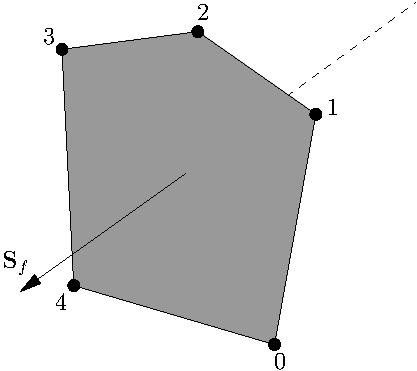
\includegraphics{fig-5-1}
 \caption{面における点の順序から決まる面領域ベクトル}
 \label{fig:5.1}
\end{figure}


面には2種類あります.
\begin{description}
 \item[内部の面]
            これらの面は必ず二つのセルに接続されており,
            その数が2を超えることはありません.
            また,内部の面において,その法線方向ベクトルが,
            より大きなラベルをもつセルに向くように,
            点のラベルの番号付けがなされます.
            つまり,セル2とセル5を接続している面だったら,
            その法線はセル5を向くわけです.
 \item[境界の面]
            これらは領域の境界にあるので,一つのセルにしか属しません.
            したがって,ある境界の面を参照するのは,
            一つのセルと境界パッチだけです.
            点ラベルの番号付けは,
            面の法線が計算領域の外側に向くように設定されます.
\end{description}

\subsubsection{セル}
\label{sssec:5.1.1.3}
セルは,面を任意の順序で並べたものです.セルは以下に示す性質が必ず必要です.
\begin{description}
 \item[切れ目なく連続である]
            セル群は計算領域全体を完全にカバーしており,
            かつ,お互いに重複してはなりません.
 \item[凸である]
            全てのセルは凸で,かつ,
            セル中心はセルの内側にある必要があります.
 \item[閉じている]
            全てのセルは幾何的にも位相的(トポロジ的)にも
            閉じていなければなりません.
            ここで,セルが幾何的に閉じているためには,
            全ての面領域ベクトルがセルの外側を向いているとして,
            それらのベクトル和が,正確にゼロ・ベクトルとなる必要があります.
            また,セルが位相的に閉じているためには,
            問題において,セル中の全ての辺が,
            二つの面により使用されている必要があります.
 \item[直交性がある]
            メッシュ内部の全ての面に対し,中心間ベクトルというのを,
            隣接する二つのセルの中心間を,
            小さいほうのラベルのセル中心から大きいほうのラベルの
            セル中心への向きで結んだベクトルとして定義することができます.
            直交性の制約というのは,内部の全ての面に対し,
            先に述べた面の面積ベクトルと中心間ベクトルのなす角が,
            常に$90\unit*{\degree}$未満であることをいいます.
\end{description}

\subsubsection{境界}
\label{sssec:5.1.1.4}
境界というのはパッチのリスト(集合)であり,
これら一つ一つは,ある境界条件が割り当てられています.
ここで,パッチというのは面のラベルのリストであり,
境界の面のみで形成され,内部の面を含みません.
この境界は閉じていることが条件であるので,
境界における全面領域ベクトルの和は,数値計算上ゼロ・ベクトルになります.


\subsection{\OFclass{polyMesh}の記述}
\label{ssec:5.1.2}
\OFpath{constant}ディレクトリのサブディレクトリである
\OFpath{polyMesh}には,
そのケースの
\index{polyMesh@\OFclass{polyMesh}!クラス}%
\index{クラス!polyMesh@\OFclass{polyMesh}}%
\OFclass{polyMesh}データが全て収められています.
このpolyMeshの記述は面ベースであり,既に述べましたように,
内部のセルは二つのセルと接続し,境界面はセルと境界のパッチを指定します.
各面には「保有」セルと「隣接」セルが割り当てられ,
面を通じた接続は,保有セルと隣接セルのラベルによって
簡潔に記述することができます.
境界の場合には,面に接続されたセルがその面の保有者であり,
隣接セルには$-1$のラベルが割り充てられます.
以上を踏まえた上で,以下のファイルで構成される入出力の詳細をご覧ください.
\begin{description}
 \item[\OFdictionary{points}]
\index{points@\OFdictionary{points}!ディクショナリ}%
\index{ディクショナリ!points@\OFdictionary{points}}%
            セルの頂点を記述するベクトルのリストです.
            ここで,リストにおける最初のベクトルは頂点$0$,
            次のベクトルの頂点$1$という風に番号付けします.
 \item[\OFdictionary{faces}]
\index{faces@\OFdictionary{faces}!ディクショナリ}%
\index{ディクショナリ!faces@\OFdictionary{faces}}%
            面のリストです.各面は点中の頂点の番号のリストで
            成り立ってます.ここで,先程と同様に,
            リスト中の最初の面の番号は$0$です.
 \item[\OFdictionary{owner}]
\index{owner@\OFdictionary{owner}!ディクショナリ}%
\index{ディクショナリ!owner@\OFdictionary{owner}}%
            保有セルのラベルのリストです.
            面のリストと同じ順番に並んでますので,
            リストの最初のラベルは$0$番の面の保有セルのラベル,
            次のラベルは$1$番の面の保有セルのラベルということになります.
 \item[\OFdictionary{neighbour}]
\index{neighbour@\OFdictionary{neighbour}!ディクショナリ}%
\index{ディクショナリ!neighbour@\OFdictionary{neighbour}}%
            隣接セルのラベルのリストです.
 \item[\OFdictionary{boundary}]
\index{boundary@\OFdictionary{boundary}!ディクショナリ}%
\index{ディクショナリ!boundary@\OFdictionary{boundary}}%
            パッチのリストです.以下のように,
            パッチ名の宣言で始まる各パッチに対するディクショナリで構成されます.
\begin{OFverbatim}[file]
movingWall
{
    type patch;
    nFaces 20;
    startFace 760;
}
\end{OFverbatim}
\index{startFace@\OFkeyword{startFace}!キーワード}%
\index{キーワード!startFace@\OFkeyword{startFace}}%
            \OFkeyword{startFace}はそのパッチにおける最初の面のラベル番号です.
            また
\index{nFaces@\OFkeyword{nFaces}!キーワード}%
\index{キーワード!nFaces@\OFkeyword{nFaces}}%
            \OFkeyword{nFaces}は,そのパッチ中の面数です.
\end{description}
備考:計算対象にいくつセルがあるか知りたい場合には,
\OFpath{owner}ファイルの\OFkeyword{FoamFile}ヘッダにおける
\OFkeyword{nCells}を見てください.


\subsection{\OFtool{cellShape}ツール}
\label{ssec:5.1.3}
別の標準的(でより単純)なメッシュ形式を,
OpenFOAMのライブラリで扱えるように変換する際に,
特に必要となるであろう\OFtool{cellShape}というツールについても説明しておきたいと思います.

多くのメッシュ・ジェネレータや後処理システムは,
実際にあり得る多面体セルの形状種類に対し,
その一部だけをサポートするものがほとんどです.
それらは,メッシュをセル形状セットといった,
3次元のセル幾何形状の限られた組み合わせで定義します.
OpenFOAMのライブラリには,
これらの一般的な形状集の定義がありますので,
上記のようなメッシュを先の節で述べたpolyMesh形式に変換することができます.

OpenFOAMによってサポートされるcellShapeモデルを
\autoref{tbl:5.1}に示します.
形状は,形状モデルにおける番号付けスキームに従って付けれらた
頂点ラベルの順序によって定義されます.
点や面,辺に対する番号付けスキームも\autoref{tbl:5.1}に書いてあります.
点の番号付けは,形状がねじれたり,
他の形状に変化することがないようにしなければならないので,
同じ点番号は複数回使用できないことになります.
さらに,重複した点はOpenFOAMでは使う必要はありません.
なぜなら,OpenFOAMで使用可能な形状は,六面体の変種を全てカバーしているからです.

セルの記述は,セルモデルの名前と,
ラベルの順序リストという二つの部分より行います.例えば,以下の点のリストを使うと,
\begin{OFverbatim}[file]
8
    (
        (0 0 0)
        (1 0 0)
        (1 1 0)
        (0 1 0)
        (0 0 0.5)
        (1 0 0.5)
        (1 1 0.5)
        (0 1 0.5)
    )
\end{OFverbatim}
六面体セルは以下のように書けます.
\begin{OFverbatim}[file]
(hex 8(0 1 2 3 4 5 6 7))
\end{OFverbatim}
ここで,六面体セルの形状は\OFkeyword{hex}というキーワードで記述しましたが,
他の形状については,\autoref{tbl:5.1}に示したキーワードを使って記述できます.


\begin{table}[p]
 %#! platex UserGuideJa
\begin{tabular}{llccc}
 セルタイプ & キーワード & 点の番号付け & 面の番号付け & 辺の番号付け \\
 \hline
 \tblstrut
 六面体 & \OFkeyword{hex}
     & 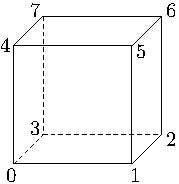
\includegraphics{tbl-5-1-1-v}
         & 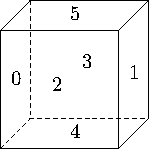
\includegraphics{tbl-5-1-1-f}
             & 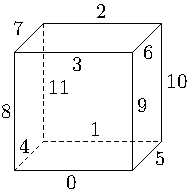
\includegraphics{tbl-5-1-1-e} \\
 くさび形 & \OFkeyword{wedge}
     & 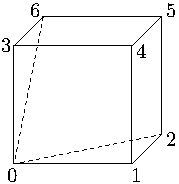
\includegraphics{tbl-5-1-2-v}
         & 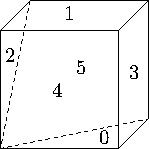
\includegraphics{tbl-5-1-2-f}
             & 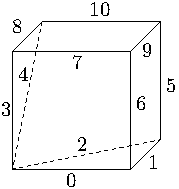
\includegraphics{tbl-5-1-2-e} \\
 三角柱 & \OFkeyword{prism}
     & 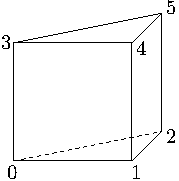
\includegraphics{tbl-5-1-3-v}
         & 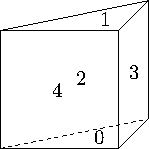
\includegraphics{tbl-5-1-3-f}
             & 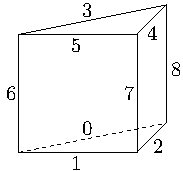
\includegraphics{tbl-5-1-3-e} \\
 四角錐 & \OFkeyword{pyr}
     & 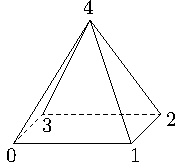
\includegraphics{tbl-5-1-4-v}
         & 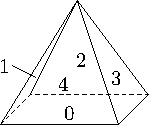
\includegraphics{tbl-5-1-4-f}
             & 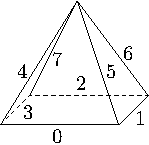
\includegraphics{tbl-5-1-4-e} \\
 四面体 & \OFkeyword{tet}
     & 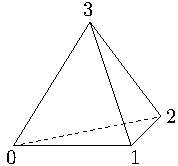
\includegraphics{tbl-5-1-5-v}
         & 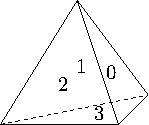
\includegraphics{tbl-5-1-5-f}
             & 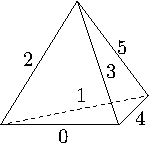
\includegraphics{tbl-5-1-5-e} \\
 くさび状四面体 & \OFkeyword{tetWedge}
     & 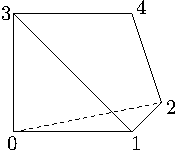
\includegraphics{tbl-5-1-6-v}
         & \includegraphics{tbl-5-1-6-f}
             & \includegraphics{tbl-5-1-6-e} \\
 \hline
\end{tabular}

 \caption{\OFtool{cellShapes}における頂点,面,辺の番号付け}
 \label{tbl:5.1}
\end{table}


\subsection{1次元や2次元,軸対称問題}
\label{ssec:5.1.4}
\index{1じげん@1次元!メッシュ}%
\index{メッシュ!1じげん@1次元}%
\index{2じげん@2次元!メッシュ}%
\index{メッシュ!2じげん@2次元}%
\index{1D!メッシュ}%
\index{メッシュ!1D}%
\index{2D!メッシュ}%
\index{メッシュ!2D}%
OpenFOAMは3次元の空間用に設計されており,
全てのメッシュもそのように定義します.
しかしながら,OpenFOAMでは,1次元や2次元
そして%
\index{じくたいしょう@軸対称!メッシュ}%
\index{メッシュ!じくたいしょう@軸対称}%
軸対称問題も解くことができ,
それには,法線方向が意図する方向であるパッチに対して,
特殊な境界条件を適用します.
具体的には,1次元や2次元問題では
\index{empty@\OFboundary{empty}!きょうかいじょうけん@境界条件}%
\index{きょうかいじょうけん@境界条件!empty@\OFboundary{empty}}%
\OFboundary{empty}のパッチタイプを使い,
軸対称問題では
\index{wedge@\OFboundary{wedge}!きょうかいじょうけん@境界条件}%
\index{きょうかいじょうけん@境界条件!wedge@\OFboundary{wedge}}%
\OFboundary{wedge}タイプを使います.
両者の使用法については\autoref{ssec:5.2.2}で触れ,
軸対称問題用の\OFkeyword{wedge}幾何形状の生成法については
\autoref{ssec:5.3.3}において述べます.



\section{境界}
\label{sec:5.2}
\index{きょうかい@境界}%
本節では境界について述べます.
境界はやや複雑です.なぜなら,形状の構成によって規定される
単純なものではなく,境界条件や境界間の接続を通して
解法を規定する不可欠の部分であるためです.
境界はメッシュ,物理量,離散化,計算法といった
多くの要素に関連しており,便宜上この章で扱います.

まず考えるべきことは,境界条件の適用のために,
境界はバラバラにされてパッチの組み合わせになるということです.
一つのパッチは一つ以上の境界面に閉じられた領域をもち,
それらが物理的に接続している必要はありません.

下に階層を示すように,パッチに関する性質は3種類あり,
\autoref{fig:5.2}では各レベルにおけるさまざまな
パッチの名前を挙げています.
下で示す階層はOpenFOAMライブラリの階層構造と類似しています.
\begin{description}
 \item[Base type(基底型)]
            形状や情報の伝達を規定
 \item[Primitive type (基本型)]
            物理量の境界条件を規定
 \item[Derived type(派生型)]
            Primitive typeから派生した,複雑な境界条件を規定
\end{description}
\OFrevision{【要検討】baseとprimitiveの訳しかた}


\begin{figure}[ht]
 \includegraphics{fig-5-2}
 \caption{境界タイプの階層}
 \label{fig:5.2}
\end{figure}


\subsection{パッチの形式の類型化}
\label{ssec:5.2.1}
パッチの種類はメッシュと物理量のファイルに規定されます.
もう少し正確にいえば,
\begin{itemize}
 \item 基底型は\OFpath{constant/polyMesh}ディレクトリにある
       \OFpath{boundary}ファイル内の各パッチに対応する
\index{type@\OFkeyword{type}!キーワード}%
\index{キーワード!type@\OFkeyword{type}}%
       \OFkeyword{type}キーワードに従って記述されます.
 \item 数値パッチ型は,基本型または派生型となり,
       フィールドファイルの各パッチに対応する
\index{type@\OFkeyword{type}!キーワード}%
\index{キーワード!type@\OFkeyword{type}}%
       \OFkeyword{type}キーワードに従って記述されます.
\end{itemize}
例として\OFtool{sonicFoam}のケースにおける\OFpath{boundary}ファイルと
\OFpath{p}ファイル(圧力物理量ファイル)を示します.
\begin{OFverbatim}[file, linenum=17]

6
(
    inlet
    {
        type            patch;
        nFaces          50;
        startFace       10325;
    }
    outlet
    {
        type            patch;
        nFaces          40;
        startFace       10375;
    }
    bottom
    {
        type            symmetryPlane;
        nFaces          25;
        startFace       10415;
    }
    top
    {
        type            symmetryPlane;
        nFaces          125;
        startFace       10440;
    }
    obstacle
    {
        type            patch;
        nFaces          110;
        startFace       10565;
    }
    defaultFaces
    {
        type            empty;
        nFaces          10500;
        startFace       10675;
    }
)

// ************************************************************************* //
\end{OFverbatim}
\begin{OFverbatim}[file, linenum=17]
dimensions      [1 -1 -2 0 0 0 0];

internalField   uniform 1;

boundaryField
{
    inlet
    {
        type            fixedValue;
        value           uniform 1;
    }

    outlet
    {
        type            waveTransmissive;
        field           p;
        phi             phi;
        rho             rho;
        psi             psi;
        gamma           1.4;
        fieldInf        1;
        lInf            3;
        value           uniform 1;
    }

    bottom
    {
        type            symmetryPlane;
    }

    top
    {
        type            symmetryPlane;
    }

    obstacle
    {
        type            zeroGradient;
    }

    defaultFaces
    {
        type            empty;
    }
}

// ************************************************************************* //
\end{OFverbatim}
\OFpath{boundary}ファイルにおける\OFkeyword{type}には,
\OFkeyword{symmetryPlane}や\OFkeyword{empty}といった
形態的制約を受けるパッチを除くすべてのパッチに対し
\OFkeyword{patch}と記述されています.
\OFpath{p}ファイルには\OFkeyword{inlet}や
\OFkeyword{bottom}といった面に適用される基本型と
\OFkeyword{outlet}に適用される複雑な派生型が記述されています.
二つのファイルを比較すると,単純な\OFkeyword{patch}ではなく,
\OFkeyword{symmetryPlane}や\OFkeyword{empty}である場合,
基底型及び数値型で一致していることがわかります.


\subsection{ 基底型}
\label{ssec:5.2.2}
以下に基底型の種類を挙げます.
これらを規定するキーワードは\autoref{tbl:5.2}にまとめてあります.


\begin{figure}[ht]
 \includegraphics{fig-5-3}
 \caption{\OFkeyword{wedge}パッチを利用した軸対象形状}
 \label{fig:5.3}
\end{figure}


\begin{table}[ht]
 %#! platex UserGuideJa
\begin{tabular}{ll}
 種類 & 意味 \\
 \hline
\index{patch@\OFkeyword{patch}!キーワードエントリ}%
\index{キーワードエントリ!patch@\OFkeyword{patch}}%
 \OFkeyword{patch} & 一般的なパッチ \\
\index{symmetryPlane@\OFkeyword{symmetryPlane}!キーワードエントリ}%
\index{キーワードエントリ!symmetryPlane@\OFkeyword{symmetryPlane}}%
 \OFkeyword{symmetryPlane} & 対称面 \\
\index{empty@\OFkeyword{empty}!キーワードエントリ}%
\index{キーワードエントリ!empty@\OFkeyword{empty}}%
 \OFkeyword{empty} & 2次元形状の前後の面 \\
\index{wedge@\OFkeyword{wedge}!キーワードエントリ}%
\index{キーワードエントリ!wedge@\OFkeyword{wedge}}%
 \OFkeyword{wedge} & 軸対称形状のための,くさび型の前後 \\
\index{cyclic@\OFkeyword{cyclic}!キーワードエントリ}%
\index{キーワードエントリ!cyclic@\OFkeyword{cyclic}}%
 \OFkeyword{cyclic} & 周期境界面 \\
\index{wall@\OFkeyword{wall}!キーワードエントリ}%
\index{キーワードエントリ!wall@\OFkeyword{wall}}%
 \OFkeyword{wall} & 壁面(乱流の壁関数に使用) \\
\index{processor@\OFkeyword{processor}!キーワードエントリ}%
\index{キーワードエントリ!processor@\OFkeyword{processor}}%
 \OFkeyword{processor} & 並列計算時のプロセッサ間の境界 \\
 \hline
\end{tabular}

 \caption{基底型の境界の種類}
 \label{tbl:5.2}
\end{table}


\begin{figure}[ht]
 \includegraphics{fig-5-4}
 \caption{\OFkeyword{cyclic}パッチを利用した周期境界の連続形状}
 \label{fig:5.4}
\end{figure}


\begin{description}
 \item[\OFboundary{patch}]
\index{patch@\OFboundary{patch}!きょうかいじょうけん@境界条件}%
\index{きょうかいじょうけん@境界条件!patch@\OFboundary{patch}}%
            メッシュに対する形状的,
            位相的情報をなにももたないパッチ条件のための
            基礎的なパッチ (\OFkeyword{wall}の場合を除く).
            流入口や流出口など.
 \item[\OFboundary{wall}]
\index{wall@\OFboundary{wall}!きょうかいじょうけん@境界条件}%
\index{きょうかいじょうけん@境界条件!wall@\OFboundary{wall}}%
            特に専門家が壁の境界を規定するときに,
            壁に適合するパッチが以下のように
            特定可能である必要がある場合があります.
            良い例としては,壁が\OFkeyword{wall}パッチの型で
            特定されなければならない壁乱流モデルがあり,
            壁に隣接するセルの中心からの距離がパッチの一部として格納されます.
 \item[\OFboundary{symmetryPlane}]
\index{symmetryPlane@\OFboundary{symmetryPlane}!きょうかいじょうけん@境界条件}%
\index{きょうかいじょうけん@境界条件!symmetryPlane@\OFboundary{symmetryPlane}}%
            対称面
 \item[\OFboundary{empty}]
\index{empty@\OFboundary{empty}!きょうかいじょうけん@境界条件}%
\index{きょうかいじょうけん@境界条件!empty@\OFboundary{empty}}%
            OpenFOAMが常に3次元で形状を生成する一方で,
            2次元(1次元)を解くことも可能です.
            そのためには,解が必要とされない3番目(2番目)の次元に
            法線が向いている各パッチに特別な\OFkeyword{empty}条件を当てはめます.
 \item[\OFboundary{wedge}]
\index{wedge@\OFboundary{wedge}!きょうかいじょうけん@境界条件}%
\index{きょうかいじょうけん@境界条件!wedge@\OFboundary{wedge}}%
            シリンダのような2次元の%
\index{じくたいしょう@軸対称!もんだい@問題}%
            軸対称問題では,
            \autoref{fig:5.3}で示すように,
            小さい角度 (例えば$< 5\unit*{\degree}$) のくさびで,
            座標面の一つにまたがる対称面に沿って伸びている
            一つのセルとして形状が記述されます.
            軸対称くさび面は\OFkeyword{wedge}型という独自のパッチである必要があります.
            \OFtool{blockMesh}を使ったくさびの形状の生成に関する詳細は
            \autoref{ssec:5.3.3}に述べられています.
 \item[\OFboundary{cyclic}]
\index{cyclic@\OFboundary{cyclic}!きょうかいじょうけん@境界条件}%
\index{きょうかいじょうけん@境界条件!cyclic@\OFboundary{cyclic}}%
            熱交換管のような繰り返しの多い形状では,
            二つのパッチをあたかも一つのように扱うことができるようにする場合があります.
            単一の\OFkeyword{cyclic}パッチは,
            \OFkeyword{faceList}において面を二つに分割します.
            そして\autoref{fig:5.4}に示すように,
            二つの面のセットを結び付けます.
            面の各組は同じ領域のものである必要がありますが,
            同じ方向のものである必要はありません.
 \item[\OFboundary{processor}]
\index{processor@\OFboundary{processor}!きょうかいじょうけん@境界条件}%
\index{きょうかいじょうけん@境界条件!processor@\OFboundary{processor}}%
            数多くの処理の中で,計算が平行して行われている場合は,
            だいたい同じ数の格子を各処理が計算するために,
            メッシュは分けられる必要があります.
            メッシュの中の異なる部分間の境界は\OFkeyword{processor}境界とよばれます.
\end{description}


\subsection{基本型}
\label{ssec:5.2.3}
\autoref{tbl:5.3}に基本型の種類を挙げます.


\begin{table}[ht]
 %#! platex UserGuideJa
\begin{tabularx}{\textwidth}{lXp{8zw}}
 種類 & 物理量$\phi$に対して与える条件 & Data to specify \\
 \hline
\index{fixedValue@\string\OFboundary{fixedValue}!きょうかいじょうけん@境界条件}%
\index{きょうかいじょうけん@境界条件!fixedValue@\string\OFboundary{fixedValue}}%
 \OFboundary{fixedValue} & $\phi$の値が一定 & \OFkeyword{value} \\
\index{fixedGradient@\string\OFboundary{fixedGradient}!きょうかいじょうけん@境界条件}%
\index{きょうかいじょうけん@境界条件!fixedGradient@\string\OFboundary{fixedGradient}}%
 \OFboundary{fixedGradient} & $\phi$の勾配が一定 & \OFkeyword{gradient} \\
\index{zeroGradient@\string\OFboundary{zeroGradient}!きょうかいじょうけん@境界条件}%
\index{きょうかいじょうけん@境界条件!zeroGradient@\string\OFboundary{zeroGradient}}%
 \OFboundary{zeroGradient} & $\phi$の勾配が$0$ & -- \\
\index{calculated@\string\OFboundary{calculated}!きょうかいじょうけん@境界条件}%
\index{きょうかいじょうけん@境界条件!calculated@\string\OFboundary{calculated}}%
 \OFboundary{calculated} & $\phi$の境界条件が他の物理量から決まる & -- \\
\index{mixed@\string\OFboundary{mixed}!きょうかいじょうけん@境界条件}%
\index{きょうかいじょうけん@境界条件!mixed@\string\OFboundary{mixed}}%
 \OFboundary{mixed} & \OFboundary{fixedValue}と\OFboundary{fixedGradient}の組み合わせ,
     \OFkeyword{valueFraction}に依存する条件 &
         \OFkeyword{refValue},\hfil\break
\index{refGradient@\string\OFkeyword{refGradient}!キーワード}%
\index{キーワード!refGradient@\string\OFkeyword{refGradient}}%
         \OFkeyword{refGradient},\hfil\break
\index{valueFraction@\string\OFkeyword{valueFraction}!キーワード}%
\index{キーワード!valueFraction@\string\OFkeyword{valueFraction}}%
         \OFkeyword{valueFraction},\hfil\break
\index{value@\string\OFkeyword{value}!キーワード}%
\index{キーワード!value@\string\OFkeyword{value}}%
         \OFkeyword{value} \\
\index{directionMixed@\string\OFboundary{directionMixed}!きょうかいじょうけん@境界条件}%
\index{きょうかいじょうけん@境界条件!directionMixed@\string\OFboundary{directionMixed}}%
 \OFboundary{directionMixed} &
     \OFrevision*{要再訳}%
     例えば法線方向と接線方向の異なるレベルでの組み合わせのような,
     テンソルの\OFkeyword{valueFraction}に対しては\OFkeyword{mixed}条件 &
         \OFkeyword{refValue},\hfil\break
         \OFkeyword{refGradient},\hfil\break
         \OFkeyword{valueFraction},\hfil\break
         \OFkeyword{value} \\
 \hline
\end{tabularx}

 \caption{基本型のパッチの種類}
 \label{tbl:5.3}
\end{table}


\subsection{派生型}
\label{ssec:5.2.4}
OpenFOAMには多数の派生型境界条件があり,ここには掲載しきれません.
かわりに,ごく一部を\autoref{tbl:5.4}に紹介します.
利用できる全てのモデルの一覧を得たければ,
OpenFOAMのソースコードを参照してください.
派生型境界条件のソースコードは以下のような場所に見つかります.
\begin{itemize}
 \item \OFpath{\$FOAM SRC/finiteVolume/fields/fvPatchFields/derived}の中
 \item 特定のモデルライブラリの中.
       これはターミナルで以下のようなコマンドを実行することで探せます.
\begin{OFverbatim}{terminal}
find $FOAM_SRC -name "*derivedFvPatch*"
\end{OFverbatim}%$
 \item 特定のソルバの中.
       これはターミナルで以下のようなコマンドを実行することで探せます.
\begin{OFverbatim}{terminal}
find $FOAM_SOLVERS -name "*fvPatch*"
\end{OFverbatim}%$
\end{itemize}



\begin{table}[p]
 \rotatebox{90}{%
 \small
 \begin{minipage}{\textheight}
  %#! platex UserGuideJa
\begin{tabularx}{\textheight}{lXp{9zw}}
 \OFboundary{fixedValue}から派生 & 意味 & 指定するデータ \\
 \hline
\index{movingWallVelocity@\string\OFboundary{movingWallVelocity}!きょうかいじょうけん@境界条件}%
\index{きょうかいじょうけん@境界条件!movingWallVelocity@\string\OFboundary{movingWallVelocity}}%
 \OFboundary{movingWallVelocity} &
     ノーマルパッチの値を置き換えるのでパッチのフラックスは$0$ & \OFkeyword{value} \\
\index{pressureInletVelocity@\string\OFboundary{pressureInletVelocity}!きょうかいじょうけん@境界条件}%
\index{きょうかいじょうけん@境界条件!pressureInletVelocity@\string\OFboundary{pressureInletVelocity}}%
 \OFboundary{pressureInletVelocity} &
     流入口の$p$が分かっているとき,$\bm{U}$は,フラックスから評価され,
     パッチはノーマル. & \OFkeyword{value} \\
\index{pressureDirectedInletVelocity@\string\OFboundary{pressureDirectedInletVelocity}!きょうかいじょうけん@境界条件}%
\index{きょうかいじょうけん@境界条件!pressureDirectedInletVelocity@\string\OFboundary{pressureDirectedInletVelocity}}%
 \OFboundary{pressureDirectedInletVelocity} &
     流入口の$p$が分かっているとき,$\bm{U}$は,
     \OFkeyword{inletDirection}のフラックスから計算される. &
         \OFkeyword{value},\OFkeyword{inletDirection} \\
\index{surfaceNormalFixedValue@\string\OFboundary{surfaceNormalFixedValue}!きょうかいじょうけん@境界条件}%
\index{きょうかいじょうけん@境界条件!surfaceNormalFixedValue@\string\OFboundary{surfaceNormalFixedValue}}%
 \OFboundary{surfaceNormalFixedValue} &
     大きさによって,ベクトル境界条件をノーマルパッチに指定します.
     ベクトルの+veはドメインを指す. & \OFkeyword{value} \\
\index{totalPressure@\string\OFboundary{totalPressure}!きょうかいじょうけん@境界条件}%
\index{きょうかいじょうけん@境界条件!totalPressure@\string\OFboundary{totalPressure}}%
 \OFboundary{totalPressure} &
     全圧$p_{0} = p + \frac{1}{2}\rho|\bm{U}|^{2}$は固定.
     $\bm{U}$が変わるとそれに従い$p$も調整される. & \OFkeyword{p0} \\
\index{turbulentInlet@\string\OFboundary{turbulentInlet}!きょうかいじょうけん@境界条件}%
\index{きょうかいじょうけん@境界条件!turbulentInlet@\string\OFboundary{turbulentInlet}}%
 \OFboundary{turbulentInlet} &
     平均値のスケールに基づく変動変数について計算する &
         \OFkeyword{referenceField}, \OFkeyword{fluctuationScale} \\
 \\
 \OFboundary{fixedGradient}/\OFboundary{zeroGradient}から派生 \\
 \hline
\index{fluxCorrectedVelocity@\string\OFboundary{fluxCorrectedVelocity}!きょうかいじょうけん@境界条件}%
\index{きょうかいじょうけん@境界条件!fluxCorrectedVelocity@\string\OFboundary{fluxCorrectedVelocity}}%
 \OFboundary{fluxCorrectedVelocity} &
     フラックスから流入口の$\bm{U}$の法線成分を計算する &
         \OFkeyword{value} \\
\index{wallBuoyantPressure@\string\OFboundary{wallBuoyantPressure}!きょうかいじょうけん@境界条件}%
\index{きょうかいじょうけん@境界条件!wallBuoyantPressure@\string\OFboundary{wallBuoyantPressure}}%
 \OFboundary{wallBuoyantPressure} &
     気圧勾配に基づく\OFboundary{fixedGradient}圧を設定する & --- \\
 \\
 \OFboundary{mixed}から派生 \\
 \hline
\index{inletOutlet@\string\OFboundary{inletOutlet}!きょうかいじょうけん@境界条件}%
\index{きょうかいじょうけん@境界条件!inletOutlet@\string\OFboundary{inletOutlet}}%
 \OFboundary{inletOutlet} &
     $\bm{U}$の向きによって\OFboundary{fixedValue}と
     \OFboundary{zeroGradient}の間で$\bm{U}$と$p$を切り替える &
         \OFkeyword{inletValue},\OFkeyword{value} \\
\index{outletInlet@\string\OFboundary{outletInlet}!きょうかいじょうけん@境界条件}%
\index{きょうかいじょうけん@境界条件!outletInlet@\string\OFboundary{outletInlet}}%
 \OFboundary{outletInlet} &
     $\bm{U}$の向きによって\OFboundary{fixedValue}と
     \OFboundary{zeroGradient}の間で$\bm{U}$と$p$を切り替える &
         \OFkeyword{outletValue},\OFkeyword{value} \\
 \OFboundary{pressureInletOutletVelocity} &
     \OFboundary{pressureInletVelocity}と
     \OFboundary{inletOutlet}の組み合わせ & \OFkeyword{value} \\
 \OFboundary{pressureDirectedInletOutletVelocity} &
     \OFboundary{pressureDirectedInletVelocity}と\OFboundary{inletOutlet}の組み合わせ &
         \OFkeyword{value},\OFkeyword{inletDirection} \\
\index{pressureTransmissive@\string\OFboundary{pressureTransmissive}!きょうかいじょうけん@境界条件}%
\index{きょうかいじょうけん@境界条件!pressureTransmissive@\string\OFboundary{pressureTransmissive}}%
 \OFboundary{pressureTransmissive} &
     周囲の圧力$p_{\infty}$に超音速圧縮波を伝える & \OFkeyword{pInf} \\
\index{supersonicFreeStream@\string\OFboundary{supersonicFreeStream}!きょうかいじょうけん@境界条件}%
\index{きょうかいじょうけん@境界条件!supersonicFreeStream@\string\OFboundary{supersonicFreeStream}}%
 \OFboundary{supersonicFreeStream} &
     斜めの衝撃を$p_{\infty}$,$T_{\infty}$,$U_{\infty}$の環境に伝える &
         \OFkeyword{pInf},\OFkeyword{TInf},\OFkeyword{UInf} \\
 その他 \\
 \hline
\index{slip@\string\OFboundary{slip}!きょうかいじょうけん@境界条件}%
\index{きょうかいじょうけん@境界条件!slip@\string\OFboundary{slip}}%
 \OFboundary{slip} & $\phi$がスカラなら\OFboundary{zeroGradient},
     $\phi$がベクトルなら法線成分は\OFboundary{fixedValue 0}で,
     接線成分は\OFboundary{zeroGradient} & --- \\
\index{partialSlip@\string\OFboundary{partialSlip}!きょうかいじょうけん@境界条件}%
\index{きょうかいじょうけん@境界条件!partialSlip@\string\OFboundary{partialSlip}}%
 \OFboundary{partialSlip} &
     混合\OFboundary{zeroGradient}/\OFboundary{slip}条件は
     \OFkeyword{valueFraction}による.\OFboundary{slip}ならば$1$. &
         \OFkeyword{valueFraction} \\
 \hline
\end{tabularx}

  Note: $p$は圧力, $\bm{U}$は速度
  \caption{派生型の種類}
  \label{tbl:5.4}
 \end{minipage}}
\end{table}



\section{\OFtool{blockMesh}ユーティリティを使ったメッシュ生成}
\label{sec:5.3}
\index{blockMesh@\OFtool{blockMesh}!ユーティリティ}%
\index{ユーティリティ!blockMesh@\OFtool{blockMesh}}%
\index{メッシュ!せいせい@生成}%
このセクションでは,OpenFOAMとともに供給される
メッシュ生成ユーティリティの\OFtool{blockMesh}について説明します.
\OFtool{blockMesh}ユーティリティは,
\index{メッシュ!こうばいづけ@勾配付け}%
勾配付けや曲がった辺を使ったパラメトリックなメッシュを作成します.

メッシュはケースの\OFpath{constant/polyMesh}ディレクトリに位置する
\index{blockMeshDict@\OFdictionary{blockMeshDict}!ディクショナリ}%
\index{ディクショナリ!blockMeshDict@\OFdictionary{blockMeshDict}}%
\OFdictionary{blockMeshDict}というディクショナリファイルから生成します.
\OFtool{blockMesh}はこのディクショナリを読み込んでメッシュを生成し,
同じディレクトリの
\index{points@\OFdictionary{points}!ディクショナリ}%
\index{ディクショナリ!points@\OFdictionary{points}}%
\OFdictionary{points},
\index{faces@\OFdictionary{faces}!ディクショナリ}%
\index{ディクショナリ!faces@\OFdictionary{faces}}%
\OFdictionary{faces},
\index{cells@\OFdictionary{cells}!ディクショナリ}%
\index{ディクショナリ!cells@\OFdictionary{cells}}%
\OFdictionary{cells}および
\index{boundary@\OFdictionary{boundary}!ディクショナリ}%
\index{ディクショナリ!boundary@\OFdictionary{boundary}}%
\OFdictionary{boundary}ファイルに
メッシュ・データを書き出します.

\OFtool{blockMesh}がよりどころとする原則は,
一つあるいは複数の3次元の六面体のブロックに領域を分割することです.
ブロックの辺は,直線,円弧またはスプラインであるかもしれません.
メッシュは,ブロックの各方向の多くのセルとして表面上指定され,
これは\OFtool{blockMesh}がメッシュ・データを生成するのに十分な情報です.

各ブロックの幾何形状は八つの頂点,
六面体の各隅のひとつによって定義されます.
頂点はラベルを使用することで各頂点にアクセスできるように
リストに書かれています. OpenFOAMは常にC++の慣習に従って,
リストの最初の要素をラベル `0' とします.
リストに従って,各頂点に番号付けがされているブロックの例を
\autoref{fig:5.5}に示します.
頂点1と5を接続する辺は,
\OFtool{blockMesh}で曲がった辺を指定できるのを
読者に思いおこさせるために曲がっています.

\autoref{ssec:5.3.3}で説明されるように,
1組以上の頂点をお互いの上で潰すことによって
八つ未満の頂点をもつブロックを生成することが可能です.

各ブロックは,
\index{ざひょうじく@座標軸!みぎてけい@右手系}
右手系である局所座標系$(x_{1}, x_{2}, x_{3})$をもちます.
右手系の軸群は,$Oz$軸を見下ろしたとき,
$Ox$軸上の点から$Oy$軸上への円弧が時計回りとなるように定義されます.
局所座標系は以下に従ってブロックの定義で提示された
頂点の順序に従って定義されます.
\begin{itemize}
 \label{p:U-130}
 \item 軸の原点はブロックの定義における最初の入力です.
       私たちの例では頂点0です.
 \item $x_{1}$の方向は,頂点0から頂点1まで動くことによって示されます.
 \item $x_{2}$の方向は,頂点1から頂点2まで動くことによって示されます.
 \item 頂点0,1,2,3は$x_{3} = 0$の平面を定義します.
 \item 頂点4は頂点0から$x_{3}$方向に動くことによって,見つけられます.
 \item 頂点5,6,および7は,頂点1,2,および3から
       それぞれ$x_{3}$の方向に動くことで,同様に見つけられます.
\end{itemize}


\begin{figure}[ht]
 \includegraphics{fig-5-5}
 \caption{ひとつのブロック}
 \label{fig:5.5}
\end{figure}


\begin{table}[ht]
 %#! platex UserGuideJa
\begin{tabularx}{\textwidth}{lXX}
 キーワード & 説明 & 指定するデータ \\
 \hline
\index{convertToMeters@\string\OFkeyword{convertToMeters}!キーワード}%
\index{キーワード!convertToMeters@\string\OFkeyword{convertToMeters}}%
 \OFkeyword{convertToMeters} &
     頂点座標の倍率 &
         \OFkeyword{0.001}とすれば$\unit*{mm}$ \\
\index{vertices@\string\OFkeyword{vertices}!キーワード}%
\index{キーワード!vertices@\string\OFkeyword{vertices}}%
 \OFkeyword{vertices} &
     頂点座標のリスト &
         \OFkeyword{(0 0 0)} \\
\index{edges@\string\OFkeyword{edges}!キーワード}%
\index{キーワード!edges@\string\OFkeyword{edges}}%
 \OFkeyword{edges} &
\index{arc@\string\OFkeyword{arc}!キーワード}%
\index{キーワード!arc@\string\OFkeyword{arc}}%
     \OFkeyword{arc}もしくは
\index{spline@\string\OFkeyword{spline}!キーワード}%
\index{キーワード!spline@\string\OFkeyword{spline}}%
     \OFkeyword{spline}の辺を書くために使用 &
         arc 1 4 (0.939 0.342 -0.5) \\
\index{block@\string\OFkeyword{block}!キーワード}%
\index{キーワード!block@\string\OFkeyword{block}}%
 \OFkeyword{block} &
     頂点ラベルとメッシュサイズの順序リスト &
         \OFkeyword{hex (0 1 2 3 4 5 6 7)}\par
         \OFkeyword{(10 10 1)}\par
         \mbox{\OFkeyword{simpleGrading (1.0 1.0 1.0)}} \\
\index{patches@\string\OFkeyword{patches}!キーワード}%
\index{キーワード!patches@\string\OFkeyword{patches}}%
 \OFkeyword{patches} &
     パッチのリスト &
         \OFkeyword{symmetryPlane base}\par
         \OFkeyword{( (0 1 2 3) )} \\
\index{mergePatchPairs@\string\OFkeyword{mergePatchPairs}!キーワード}%
\index{キーワード!mergePatchPairs@\string\OFkeyword{mergePatchPairs}}%
 \OFkeyword{mergePatchPairs} &
     マージするパッチのリスト &
         \autoref{ssec:5.3.2}参照 \\
 \hline
\end{tabularx}

 \caption{\OFdictionary{blockMeshDict}に使用するキーワード}
 \label{tbl:5.5}
\end{table}


\subsection{\OFdictionary{blockMeshDict}ファイルの記述}
\label{ssec:5.3.1}
\OFdictionary{blockMeshDict}ファイルは,
\autoref{tbl:5.5}で説明されている
キーワードを使用するディクショナリです.
\index{convertToMeters@\OFkeyword{convertToMeters}!キーワード}%
\index{キーワード!convertToMeters@\OFkeyword{convertToMeters}}%
\OFkeyword{convertToMeters}キーワードは,
メッシュ記述におけるすべての頂点の座標にかけられる
尺度因子を指定します.例えば,
\begin{OFverbatim}[file]
convertToMeters 0.001;
\end{OFverbatim}
は,すべての座標に$0.001$をかけることを意味します.
すなわち,\OFdictionary{blockMeshDict}ファイルで引用された値が$\unit*{mm}$になります.

\subsubsection{頂点}
\label{sssec:5.3.1.1}
メッシュのブロックの頂点は,
\OFkeyword{vertices}と名づけられた
標準のリストとして以下のように与えられます.
例えば\autoref{fig:5.5}での私たちの例のブロックに関しては,
頂点は以下のとおりです.
\begin{OFverbatim}[file]
vertices
(
    ( 0 0 0 ) // vertex number 0
    ( 1 0 0.1) // vertex number 1
    ( 1.1 1 0.1) // vertex number 2
    ( 0 1 0.1) // vertex number 3
    (-0.1 -0.1 1 ) // vertex number 4
    ( 1.3 0 1.2) // vertex number 5
    ( 1.4 1.1 1.3) // vertex number 6
    ( 0 1 1.1) // vertex number 7
);
\end{OFverbatim}

\subsubsection{辺}
\label{sssec:5.3.1.2}
2頂点をつなぐ辺のそれぞれは,
デフォルトでまっすぐであると仮定されています.
しかしながら,どんな辺も,
\OFkeyword{edges}と名づけられるリストにおける入力で
曲がるように指定されるかもしれません.
そのリストはオプションです.
幾何形状がどんな曲がった辺も含んでいないなら,
それは省略されるかもしれません.

曲がった辺のための各入力は,
\autoref{tbl:5.6}に挙げられているものから
カーブのタイプを指定するキーワードとともに始まります.


\begin{table}[ht]
 %#! platex UserGuideJa
\begin{tabular}{lll}
 キーワード選択 & 説明 & 追加するエントリ \\
 \hline
\index{arc@\OFkeyword{arc}!キーワードエントリ}%
\index{キーワードエントリ!arc@\OFkeyword{arc}}%
 \OFkeyword{arc} & 円弧 & 1点の補間点 \\
\index{simpleSpline@\OFkeyword{simpleSpline}!キーワードエントリ}%
\index{キーワードエントリ!simpleSpline@\OFkeyword{simpleSpline}}%
 \OFkeyword{simpleSpline} & スプライン曲線 & 補間点リスト \\
\index{polyLine@\OFkeyword{polyLine}!キーワードエントリ}%
\index{キーワードエントリ!polyLine@\OFkeyword{polyLine}}%
 \OFkeyword{polyLine} & 線群 & 補間点リスト \\
\index{polySpline@\OFkeyword{polySpline}!キーワードエントリ}%
\index{キーワードエントリ!polySpline@\OFkeyword{polySpline}}%
 \OFkeyword{polySpline} & スプライン群 & 補間点リスト \\
\index{line@\OFkeyword{line}!キーワードエントリ}%
\index{キーワードエントリ!line@\OFkeyword{line}}%
 \OFkeyword{line} & 直線 & --- \\
 \hline
\end{tabular}

 \caption{\OFdictionary{blockMeshDict}ディクショナリで使用可能なエッジタイプ}
 \label{tbl:5.6}
\end{table}


そして,キーワードの後には辺が接続する二つの頂点のラベルが続きます.
それに続いて,辺が通り過ぎる内挿点を指定しなければなりません.
\OFkeyword{arc}には,円弧が横切ることになる一つの内挿点が必要です.
\OFkeyword{simpleSpline},\OFkeyword{polyLine},
および\OFkeyword{polySpline}に関しては,内挿点のリストが必要です.
\OFkeyword{line}辺は,デフォルトとして実行されるオプションと
全く同等であり,内挿点を全く必要としません.
\OFkeyword{line}辺を使用する必要は全くありませんが,
それが完全性のために含まれていることに注意してください.
\autoref{fig:5.6}での私たちの例のブロックでは,
内挿点$(1.1, 0.0, 0.5)$を通して以下のように
頂点1と5をつなぐ\OFkeyword{arc}辺を指定します.
\begin{OFverbatim}[file]
edges
(
    arc 1 5 (1.1 0.0 0.5)
);
\end{OFverbatim}

\subsubsection{ブロック}
\label{sssec:5.3.1.3}
ブロックの定義は
\index{blocks@\OFkeyword{blocks}!キーワード}%
\index{キーワード!blocks@\OFkeyword{blocks}}%
\OFkeyword{blocks}と名づけられたリストに含まれています.
各ブロックの定義は,セクション\autoref{sec:5.3}で示された順序をもつ
頂点ラベルのリストからなる複合入力です.
ベクトルが各方向に必要なセルの数,タイプ,
および各方向のセル拡大比のリストを与えます.

そして,ブロックは以下のとおり定義されます.
\begin{OFverbatim}[file]
blocks
(
    hex (0 1 2 3 4 5 6 7) // vertex numbers
    (10 10 10) // numbers of cells in each direction
    simpleGrading (1 2 3) // cell expansion ratios
);
\end{OFverbatim}
それぞれのブロックの定義は以下のとおりです.
\begin{description}
 \item[Vertex numbering]
\index{blockMesh@\OFtool{blockMesh}!じっこうかのう@実行可能な頂点の番号付け}%
            \OFpath{OpenFOAM-1.7.1/cellModels}ファイルに
            定義されているように,最初の入力がブロックの
\index{けいじょう@形状}%
            形状識別子です.
            いつもブロックが六面体であるので,
            いつも形は\OFkeyword{hex}です.
            \pageref{p:U-130}ページで説明された方法で並べられた
            頂点番号のリストが従います.
 \item[Number of cells]
            2番目の入力はそのブロックの$x_{1}$,$x_{2}$,$x_{3}$と
            それぞれの方向のセルの数を与えます.
 \item[Cell expansion ratios]
\index{ブロック!かくだいりつ@拡大率}%
\index{セル!かくだいりつ@拡大率}%
            3番目の入力はブロックにおける各方向へのセルの拡大比を与えます.
            拡大比は,メッシュが指定された方向に段階的なものにするか,
            または精製されるのを可能にします.
            比率$\delta_{\mathrm{e}}$は\autoref{fig:5.6}に示すように,
            ブロックのひとつの辺に沿った終わりのセルの幅の,
            辺に沿った始めのセル幅$\delta_{\mathrm{s}}$への比です.
            以下のキーワードのそれぞれは\OFtool{blockMesh}で利用可能な
\index{メッシュ!こうばいづけ@勾配付け}%
            勾配付けの仕様の二つのタイプの一つを指定します.
            \begin{description}
             \item[simpleGrading]
\index{simpleGrading@\OFkeyword{simpleGrading}!キーワード}%
\index{キーワード!simpleGrading@\OFkeyword{simpleGrading}}%
                        簡単な記述で,局所的な$x_{1}$,$x_{2}$と$x_{3}$方向それぞれに一様な
                        拡大比を,三つの拡大比だけで指定します.例えば
\begin{OFverbatim}[file]
simpleGrading (1 2 3)
\end{OFverbatim}
             \item[edgeGrading]
\index{edgeGrading@\OFkeyword{edgeGrading}!キーワード}%
\index{キーワード!edgeGrading@\OFkeyword{edgeGrading}}%
                        完全なセルの拡大比の記述は,
                        \autoref{fig:5.5}に矢印で
                        「最初のセルから最後のセル」の方向を表した
                        スキームに従って番号付けられた
                        ブロックの各辺に比率を与えます.
                        例えば,このようなものです.
\begin{OFverbatim}[file]
edgeGrading (1 1 1 1 2 2 2 2 3 3 3 3)
\end{OFverbatim}
                        これは,辺$0$--$3$に沿ったセル幅の比率が$1$,
                        辺$4$--$7$に沿った比率が$2$であり,
                        辺$8$--$11$に沿った比率が$3$である
                        ということであることを意味しており,
                        上述した\OFkeyword{simpleGrading}の例に
                        まったく同等です.
            \end{description}
\end{description}


\begin{figure}[ht]
 \includegraphics{fig-5-6}
 \caption{ブロックの辺に沿って段階わけされたメッシュ}
 \label{fig:5.6}
\end{figure}


\subsubsection{パッチ}
\label{sssec:5.3.1.4}
\index{patches@\OFkeyword{patches}!キーワード}%
\index{キーワード!patches@\OFkeyword{patches}}%
\OFkeyword{patches}というリストで
メッシュのパッチを与えます.
リストにおける各パッチは以下を含む複合記入です.
\begin{itemize}
 \item パッチタイプ,いくつかの境界条件が適用されている一般的なパッチか,
       \autoref{tbl:5.1}にリストアップされていて
       セクション\autoref{ssec:5.2.2}で説明される特定の幾何的条件のどちらか.
 \item パッチを作るブロックの面のリスト,
       便利にパッチを特定できる名前が推奨されるものの,
       名前はユーザの選択に任されます.
       例えば\OFkeyword{quoteTextinlet},
       この名前は,境界条件をフィールドデータファイルに
       設定するための識別子として使用されます.
       \OFtool{blockMesh}は\OFkeyword{patches}リストから省かれる
       どんな境界パッチからも面を集め,
       それらに\OFkeyword{defaultFaces}とよばれる
       \OFkeyword{empty}タイプからなるデフォルトパッチを割り当てます.
       これは,2次元の幾何形状において,
       それらが必要に応じて\OFkeyword{empty}パッチに
       集められるのを知りながら,
       ユーザは2次元平面にあるブロック面を
       省略する選択ができることを意味します.
\end{itemize}
\autoref{fig:5.5}での例のブロックに戻って,
もし左面に流入があり,右面における流出があり,
他の四つの表面が壁であるならば,以下のとおりパッチは定義できるでしょう.
\begin{OFverbatim}[file]
patches // keyword
(
    patch // patch type for patch 0
    inlet // patch name
    (
        (0 4 7 3) // block face in this patch
    ) // end of 0th patch definition
    patch // patch type for patch 1
    outlet // arbitrary patch name
    (
        (1 2 6 5)
    )
    wall
    walls
    (
        (0 1 5 4)
        (0 3 2 1)
        (3 7 6 2)
        (4 5 6 7)
    )
);
\end{OFverbatim}
それぞれのブロック面は四つの頂点番号のリストによって定義されます.
頂点が与えられる順序は,ブロックの中から見て,
どの頂点からも始めても,他の頂点を定義するために
時計回りに面を回るようなものにならなければなりません.


\subsection{複数のブロック}
\label{ssec:5.3.2}
1ブロック以上を使用することでメッシュを作成できます.
そのような事情では,メッシュは前述のテキストで
説明されるように作成されます.
唯一の追加設定がブロック間の接続です.
そこに,二つの異なる可能性があります.
\begin{description}
 \item[face matching]
            あるブロックのパッチを包括する面の組が,
            別のブロックのパッチを包括する面の組と全く同じ位置にあるものです.
 \item[face merging]
            あるブロックのパッチからの面のグループは,
            二つのブロックをつなげながら新しい内部の面の組を作成するために,
            別のブロックのパッチからの面の別のグループに関連づけられます.
\end{description}
face matchingで2ブロックをつなげるためには,
接続を形成する二つのパッチが
\OFkeyword{patches}リストから単に無視されるべきです.
\OFtool{blockMesh}は,面が外部の境界を形成せず,
同じところに位置する各組を,2ブロックからのセルを接続する,
ひとつの内部面に結合するのを特定します.

もうひとつのface margingは,
併合されるブロックパッチがまず\OFkeyword{patches}リストで
定義されることを必要とします.面が併合されるパッチのそれぞれの組が,
\OFkeyword{mergePatchPairs}というオプションリストに含まなければなりません.
\OFkeyword{mergePatchPairs}の形式は以下のとおりです.
\begin{OFverbatim}[file]
mergePatchPairs
(
    ( <masterPatch> <slavePatch> ) // merge patch pair 0
    ( <masterPatch> <slavePatch> ) // merge patch pair 1
    ...
)
\end{OFverbatim}
パッチの組は,最初のパッチはマスタになり,
2番目はスレイブになると解釈されます.
併合するための規則は以下のとおりです
\begin{itemize}
 \item マスタパッチの面は元々定義されているままで,
       すべての頂点は元の位置にあります.
 \item スレイブパッチの面は,スレイブとは多少異なる
       マスタパッチに投影されます.
 \item スレイブ面のどんな頂点の位置も,
       面の最小許容値より短いあらゆる辺を除去するために,
       \OFtool{blockMesh}によって調整されるかもしれません.
 \item パッチが\autoref{fig:5.7}に示されるように重なるなら,
       併合しない各面が,境界条件を適用しなければならない,
       元のパッチの外部面として残ります.
 \item パッチのすべての面が併合されているなら,
       パッチ自体は表面を全く含まないので,除去されます.
\end{itemize}


\begin{figure}[ht]
 \includegraphics{fig-5-7}
 \caption{重なったパッチのマージ}
 \label{fig:5.7}
\end{figure}


結果的に,スレイブパッチのオリジナルの幾何形状が,
併合の間必ずしも,完全に保存されるというわけではないということです.
したがって,たとえば,円筒状のブロックが,
より大きいブロックにつなげられている場合では,
円筒状の形が正しく保存されるように,
マスタパッチを円筒状のブロックにするのが賢いでしょう.
併合手順を確実に成功させるためのいくつかの追加の推奨策があります.
\begin{itemize}
 \item 2次元の幾何学形状では,2次元平面の外での3次元目のセルサイズは,
       2次元平面でのセルの幅・高さと同様であるべきです.
 \item 二度パッチを併合すること,すなわち,
       \OFkeyword{mergePatchPairs}で二度それを含めるのは勧められません.
 \item 併合されるべきパッチが,他の併合されるパッチと共通の
       辺を共有するところでは,両方がマスタパッチとして宣言されるべきです.
\end{itemize}


\subsection{8頂点未満のブロックの作成}
\label{ssec:5.3.3}
八つ未満の頂点でブロックを作成するために,
1組以上の頂点をお互いの上で潰すことが可能です.
頂点を潰す最も一般的な例としては,
セクション\autoref{ssec:5.2.2}で説明した
\index{wedge@\OFboundary{wedge}!きょうかいじょうけん@境界条件}%
\index{きょうかいじょうけん@境界条件!wedge@\OFboundary{wedge}}%
\OFboundary{wedge}パッチタイプを使用する
2次元の%
\index{じくたいしょう@軸対称!もんだい@問題}%
軸対称問題のための6面のくさび型ブロックを作成するときがあります.
\autoref{fig:5.8}に示す私たちの例における,
ブロックの簡易型のバージョンを使用することで,
過程をわかりやすく例証します.
頂点7を頂点4に,頂点6を頂点5に置いて潰すことによって,
くさび型ブロックを作成したいということです.
これは,ブロック番号7を4で,6を5でそれぞれ交換することによって
簡単にできます.するとブロック番号はこのようになります.
\begin{OFverbatim}[file]
hex (0 1 2 3 4 5 5 4)
\end{OFverbatim}


\begin{figure}[ht]
 \includegraphics{fig-5-8}
 \caption{くさび形をしたブロックを六つの接点で作る}
 \label{fig:5.8}
\end{figure}


潰れている頂点を含むブロック面を考えることで,
同じことがパッチにも適用でき,以前\OFkeyword{(4 5 6 7)}だったものが,
\OFkeyword{(4 5 5 4)}になります.これは面積をもたないブロック面で,
\OFkeyword{polyMesh}で面のないパッチを生成します.
これは\OFpath{boundary}ファイルにおいて
同様の場合でも見ることができることと同じです.
パッチは\OFdictionary{blockMeshDict}で,
\OFkeyword{empty}として指定されるべきです.
そしてどんなフィールドの境界条件も結果的に\OFkeyword{empty}であるはずです.


\subsection{\OFtool{blockMesh}の実行}
\label{ssec:5.3.4}
\autoref{sec:3.3}で説明されたように,
\OFpath{<case>}ディレクトリのケースに対して
\OFtool{blockMesh}を実行するためには,
以下のようにすればコマンドラインで実行できます.
\begin{OFverbatim}[terminal]
blockMesh -case <case>
\end{OFverbatim}
\index{blockMeshDict@\OFdictionary{blockMeshDict}!ディクショナリ}%
\index{ディクショナリ!blockMeshDict@\OFdictionary{blockMeshDict}}%
\OFdictionary{blockMeshDict}ファイルは,
サブディレクトリ\OFpath{constant/polyMesh}に存在しなければなりません.



\section{\OFtool{snappyHexMesh}ユーティリティを使ったメッシュ生成}
\label{sec:5.4}
\index{snappyHexMesh@\OFtool{snappyHexMesh}!ユーティリティ}%
\index{ユーティリティ!snappyHexMesh@\OFtool{snappyHexMesh}}%
\index{メッシュ!せいせい@生成}%
OpenFOAMのメッシュ生成ユーティリティ
\OFtool{snappyHexMesh}について解説します.
\OFtool{snappyHexMesh}は
\index{Stereolithography (STL)}%
STL形式の三角の表面形状から
六面体と
\index{メッシュ!ぶんかつろくめんたい@分割六面体}%
分割六面体の3次元メッシュを自動的に生成します.
はじめのメッシュの細分化と,後に現れる分割の六進法のメッシュの
\index{ひょうめんメッシュ@表面メッシュ}%
表面形状への変形を繰り返して表面形状に近づいていきます.
オプションとして,現れたメッシュを縮小させ,
レイヤセルを挿入することができます.
メッシュの細分化のレベルは非常に柔軟性が高く,
表面の処理はあらかじめ定義したメッシュの水準に適合します.
\OFtool{snappyHexMesh}は毎回負荷を平均化して並列動作をします.


\begin{figure}[ht]
 \includegraphics{fig-5-9}
 \caption{\OFtool{snappyHexMesh}における2次元メッシュ問題の概略図}
 \label{fig:5.9}
\end{figure}


\subsection{\OFtool{snappyHexMesh}によるメッシュ生成の過程}
\label{ssec:5.4.1}
\autoref{fig:5.9}に示す概略図を用いて
メッシュを\OFtool{snappyHexMesh}によって生成する流れを説明します.
\index{メッシュ!Stereolithography (STL)}%
Stereolithography (STL) 形式の
\index{メッシュ!ひょうめん@表面}%
表面形状で描かれた対象を囲む長方形の部分
(図中のグレーの部分)にメッシュを作成することを目的とします.
これは外部の空気力学のシミュレーションにおいて典型的な手法です.
あくまでも\OFtool{snappyHexMesh}は3次元メッシュの生成ツールですが,
簡単のためここでは2次元の図を使用しています.

\OFtool{snappyHexMesh}を実行するには以下の準備が必要です.
\begin{itemize}
 \item 2進法またはASCIIで表されたSTL形式による表面形状データを
       ケースディレクトリの\OFpath{triSurface}サブディレクトリに置く.
 \item \autoref{ssec:5.4.2}で述べる\OFtool{blockMesh}を使用して,
       解析領域の範囲とメッシュ密度の基準を決めるために
       六角形の基礎メッシュを作成しておく.
 \item ケースの\OFpath{system}ディレクトリにある
\index{snappyHexMeshDict@\OFpath{snappyHexMeshDict}!ファイル}%
\index{ファイル!snappyHexMeshDict@\OFpath{snappyHexMeshDict}}%
       \OFpath{snappyHexMeshDict}ディクショナリに,適切な内容を入力する.
\end{itemize}
\OFpath{snappyHexMeshDict}ディクショナリには,
\index{snappyHexMesh@\OFtool{snappyHexMesh}!ユーティリティ!メッシュせいせいプロセス@メッシュ生成プロセス}%
メッシュ生成の様々な段階を管理する最上位での変更や,
各過程における個々のサブディレクトリがあります.
入力例を\autoref{tbl:5.7}に示します.


\begin{table}[ht]
 % #! platex UserGuideJa
\begin{tabularx}{\textwidth}{lXl}
 キーワード & 意味 & 例 \\
 \hline
\index{castellatedMesh@\string\OFkeyword{castellatedMesh}!キーワード}%
\index{キーワード!castellatedMesh@\string\OFkeyword{castellatedMesh}}%
 \OFkeyword{castellatedMesh} & 階段状のメッシュを作成するか & \OFkeyword{true} \\
\index{snap@\string\OFkeyword{snap}!キーワード}%
\index{キーワード!snap@\string\OFkeyword{snap}}%
 \OFkeyword{snap} & 表面への適合操作をするか & \OFkeyword{true} \\
\index{doLayers@\string\OFkeyword{doLayers}!キーワード}%
\index{キーワード!doLayers@\string\OFkeyword{doLayers}}%
 \OFkeyword{doLayers} & レイヤの追加をするか & \OFkeyword{true} \\
\index{mergeTolerance@\string\OFkeyword{mergeTolerance}!キーワード}%
\index{キーワード!mergeTolerance@\string\OFkeyword{mergeTolerance}}%
 \OFkeyword{mergeTolerance} &
 マージする許容値.初期メッシュのバウンディングボックスに対する比. &
 \OFkeyword{1e-06} \\
\index{debug@\string\OFkeyword{debug}!キーワード}%
\index{キーワード!debug@\string\OFkeyword{debug}}%
 \OFkeyword{debug} & 中間メッシュと画面出力の制御 \\
 & 最終メッシュのみ出力 & \OFkeyword{0} \\
 & 中間メッシュの出力 & \OFkeyword{1} \\
 & 後処理のため\OFkeyword{cellLevel}を付けた\OFkeyword{volScalarField}を出力 & \OFkeyword{2} \\
 & \OFpath{.obj}ファイルとして中間時の交線を出力 & \OFkeyword{4} \\
\index{geometry@\string\OFkeyword{geometry}!キーワード}%
\index{キーワード!geometry@\string\OFkeyword{geometry}}%
 \OFkeyword{geometry} & 使用する全表面形状のサブディクショナリ \\
\index{castellatedMeshControls@\string\OFkeyword{castellatedMeshControls}!キーワード}%
\index{キーワード!castellatedMeshControls@\string\OFkeyword{castellatedMeshControls}}%
 \OFkeyword{castellatedMeshControls} & 階段状メッシュ制御のサブディクショナリ \\
\index{snapControls@\string\OFkeyword{snapControls}!キーワード}%
\index{キーワード!snapControls@\string\OFkeyword{snapControls}}%
 \OFkeyword{snapControls} & 表面スナップ制御のサブディクショナリ \\
\index{addLayersControls@\string\OFkeyword{addLayersControls}!キーワード}%
\index{キーワード!addLayersControls@\string\OFkeyword{addLayersControls}}%
 \OFkeyword{addLayersControls} & レイヤ追加制御のサブディクショナリ \\
\index{meshQualityControls@\string\OFkeyword{meshQualityControls}!キーワード}%
\index{キーワード!meshQualityControls@\string\OFkeyword{meshQualityControls}}%
 \OFkeyword{meshQualityControls} & メッシュ品質制御のサブディクショナリ \\
 \hline
\end{tabularx}

 \caption{\OFtool{snappyHexMeshDict}の最上位のキーワード}
 \label{tbl:5.7}
\end{table}


\OFtool{snappyHexMesh}で読み込む形状は
\OFpath{snappyHexMeshDict}内の\OFkeyword{geometory}の部分に記述します.
形状はSTL形状またはOpenFOAMにおける幾何実体によって指定されます.
以下に例を示します.
\begin{OFverbatim}[file]
geometry
  {
      sphere.stl // STL filename
      {
          type triSurfaceMesh;
          regions
          {
              secondSolid             // Named region in the STL file
              {
                  name mySecondPatch; // User-defined patch name
              }                       // otherwise given sphere.stl_secondSolid
          }
      }

      box1x1x1  // User defined region name
      {
          type   searchableBox;       // region defined by bounding box
          min    (1.5 1 -0.5);
          max    (3.5 2 0.5);
      }

      sphere2  // User defined region name
      {
          type   searchableSphere;    // region defined by bounding sphere
          centre (1.5 1.5 1.5);
          radius 1.03;
      }
  };
\end{OFverbatim}


\subsection{六面体基礎メッシュの作成}
\label{ssec:5.4.2}
\OFtool{snappyHexMesh}を実行する前に\OFtool{blockMesh}を使用して
\autoref{fig:5.10}が示すように,
解析領域をカバーする六面体セルの
\index{snappyHexMesh@\OFtool{snappyHexMesh}!ユーティリティ!きそメッシュ@基礎メッシュ}%
基礎メッシュを作成します.
基礎メッシュの生成時は以下の点に注意しなければなりません.
\begin{itemize}
 \item メッシュは六面体のみで構成されていること
 \item セルのアスペクト比がほぼ$1$であること.
       少なくとも連続したスナップが行われる表面近傍で
       そうでなければスナップの収束に時間がかかり,不良の原因となる.
 \item STLの表面とセルのエッジが最低でも一箇所は交差すること.
       つまり,一つのセルだけのメッシュでは機能しない.
\end{itemize}


\begin{figure}[ht]
 \includegraphics{fig-5-10}
 \caption{\OFtool{snappyHexMesh}実行前の基礎メッシュの生成}
 \label{fig:5.10}
\end{figure}


\subsection{面と輪郭に合わせたセルの分割}
\label{ssec:5.4.3}
\index{snappyHexMesh@\OFtool{snappyHexMesh}!ユーティリティ!セルのぶんかつ@セルの分割}%
セルの分割は,\OFpath{snappyHexMeshDict}の
\index{castellatedMeshControls@\OFsubdictionary{castellatedMeshControls}!ディクショナリ}%
\index{ディクショナリ!castellatedMeshControls@\OFsubdictionary{castellatedMeshControls}}%
\OFsubdictionary{castellatedMeshControls}サブディクショナリにおいて設定して実行します.
\OFsubdictionary{castellatedMeshControls}の入力の例を\autoref{tbl:5.8}に示します.


\begin{table}[ht]
 %#! platex UserGuideJa
\begin{tabularx}{\textwidth}{lXl}
 キーワード & 意味 & 例 \\
 \hline
\index{locationInMesh@\string\OFkeyword{locationInMesh}!キーワード}%
\index{キーワード!locationInMesh@\string\OFkeyword{locationInMesh}}%
 \OFkeyword{locationInMesh} & メッシュが作成される領域内の位置ベクトル & \OFkeyword{(5 0 0)} \\
 & 位置ベクトルが細分化の前または最中にセルの面と一致してはいけない \\
\index{maxLocalCells@\string\OFkeyword{maxLocalCells}!キーワード}%
\index{キーワード!maxLocalCells@\string\OFkeyword{maxLocalCells}}%
 \OFkeyword{maxLocalCells} & 細分化中におけるプロセッサあたりのセルの数の最大値 & \OFkeyword{1e+06} \\
\index{maxGlobalCells@\string\OFkeyword{maxGlobalCells}!キーワード}%
\index{キーワード!maxGlobalCells@\string\OFkeyword{maxGlobalCells}}%
 \OFkeyword{maxGlobalCells} & 細分化中におけるセルの数の総数 (i.e. 除去の前) & \OFkeyword{2e+06} \\
\index{minRefinementCells@\string\OFkeyword{minRefinementCells}!キーワード}%
\index{キーワード!minRefinementCells@\string\OFkeyword{minRefinementCells}}%
 \OFkeyword{minRefinementCells} & 細分化すべきセルの数の最低値.この値以下だと停止 & \OFkeyword{0} \\
\index{nCellsBetweenLevels@\string\OFkeyword{nCellsBetweenLevels}!キーワード}%
\index{キーワード!nCellsBetweenLevels@\string\OFkeyword{nCellsBetweenLevels}}%
 \OFkeyword{nCellsBetweenLevels} & 異なる細分化レベル間のセルの緩衝レイヤーの数 & \OFkeyword{1} \\
\index{resolveFeatureAngle@\string\OFkeyword{resolveFeatureAngle}!キーワード}%
\index{キーワード!resolveFeatureAngle@\string\OFkeyword{resolveFeatureAngle}}%
 \OFkeyword{resolveFeatureAngle} & 角度がこの値を超えている交点をもつセルに最高レベルの細分化を行う & \OFkeyword{30} \\
\index{features@\string\OFkeyword{features}!キーワード}%
\index{キーワード!features@\string\OFkeyword{features}}%
 \OFkeyword{features} & 細分化する特徴辺のリスト \\
\index{refinementSurfaces@\string\OFkeyword{refinementSurfaces}!キーワード}%
\index{キーワード!refinementSurfaces@\string\OFkeyword{refinementSurfaces}}%
 \OFkeyword{refinementSurfaces} & 細分化する表面のディクショナリ \\
\index{refinementRegions@\string\OFkeyword{refinementRegions}!キーワード}%
\index{キーワード!refinementRegions@\string\OFkeyword{refinementRegions}}%
 \OFkeyword{refinementRegions} & 細分化する領域のディクショナリ \\
 \hline
\end{tabularx}

 \caption{\OFdictionary{snappyHexMeshDict}の
\index{castellatedMeshControls@\string\OFsubdictionary{castellatedMeshControls}!ディクショナリ}%
\index{ディクショナリ!castellatedMeshControls@\string\OFsubdictionary{castellatedMeshControls}}%
 \OFsubdictionary{castellatedMeshControls}サブディクショナリのキーワード}
 \label{tbl:5.8}
\end{table}


\autoref{fig:5.11}で示されたように,
最初に領域内で指定された輪郭に従って選択されたセルで分割が開始します.


\begin{figure}[ht]
 \includegraphics{fig-5-11}
 \caption{\OFtool{snappyHexMesh}の輪郭によるセルの分割}
 \label{fig:5.11}
\end{figure}


\OFkeyword{castellatedMeshControls}サブディクショナリの輪郭のリストにおいて
\OFpath{edgeMesh}ファイルの名前と細分化のレベルを記述します.
\begin{OFverbatim}[file]
features
  (
      {
          file "someLine.eMesh"; // file containing edge mesh
          level 2;               // level of refinement
      }
  );
\end{OFverbatim}

輪郭の細分化に続き,\autoref{fig:5.12}に示すように,
指定された表面における分割のためにセルが選択されます.


\begin{figure}[ht]
 \includegraphics{fig-5-12}
 \caption{\OFtool{snappyHexMesh}の表面によるセルの分割}
 \label{fig:5.12}
\end{figure}


\OFkeyword{castellatedMeshControls}の
\OFdictionary{refinementSurface}ディクショナリで,各STL表面のディクショナリ入力と,
型の最小,最大細分化のデフォルトレベルの指定を行います.
(\verb|<min> <max>|) 最小レベルは表面のいたるところに適用され,
最大レベルは
\index{resolveFeatureAngle@\OFkeyword{resolveFeatureAngle}!キーワード}%
\index{キーワード!resolveFeatureAngle@\OFkeyword{resolveFeatureAngle}}%
\OFkeyword{resolveFeatureAngle}に規定される
角度を超過する交点をもつセルに適用されます.

細分化はSTL表面の特定領域に対して複数回行うことができます.
領域の入力は\OFsubdictionary{regions}サブディクショナリに収められています.
各領域の入力に対するキーワードは領域の名前そのものであり,
細分化のレベルはさらにサブのディクショナリに含まれます.以下の入力例を参考にしてください.
\begin{OFverbatim}[file]
refinementSurfaces
  {
      sphere.stl
      {
          level (2 2); // default (min max) refinement for whole surface
          regions
          {
              secondSolid
              {
                  level (3 3); // optional refinement for secondSolid region
              }
          }
      }
  }
\end{OFverbatim}


\subsection{セルの除去}
\label{ssec:5.4.4}
\index{snappyHexMesh@\OFtool{snappyHexMesh}!ユーティリティ!セルのじょきょ@セルの除去}%
輪郭と表面の分割が完了するとセルの除去が始まります.
セルの除去には領域内の有界表面によって完全に囲まれる
一つ以上の範囲が必要です.
セルが保持される領域は,\OFkeyword{castellatedMeshControls}の
\index{locationInMesh@\OFkeyword{locationInMesh}!キーワード}%
\index{キーワード!locationInMesh@\OFkeyword{locationInMesh}}%
\OFkeyword{locationInMesh}キーワードに指定される
領域内の位置ベクトルによって特定されます.
セルの体積のほぼ$50\unit{\%}$以上が領域内に存在する場合保持されます.
残りのセルは\autoref{fig:5.13}に示すように除去されます.


\begin{figure}[ht]
 \includegraphics{fig-5-13}
 \caption{snappyHexMeshにおけるメッシュの除去}
 \label{fig:5.13}
\end{figure}


\subsection{特定領域内のセルの分割}
\label{ssec:5.4.5}
特定領域に含まれるセルはさらに細分化されます.
\autoref{fig:5.14}では長方形の濃いグレーの領域が該当します.
\index{castellatedMeshControls@\OFsubdictionary{castellatedMeshControls}!ディクショナリ}%
\index{ディクショナリ!castellatedMeshControls@\OFsubdictionary{castellatedMeshControls}}%
\OFsubdictionary{castellatedMeshControls}内の
\index{refinementRegions@\OFsubdictionary{refinementRegions}!キーワード}%
\index{キーワード!refinementRegions@\OFsubdictionary{refinementRegions}}%
\OFsubdictionary{refinementRegions}サブディクショナリでは,
\OFsubdictionary{geometry}サブディクショナリにおいて指定された
領域の細分化の入力を行います.細分化の
\index{mode@\OFkeyword{mode}!キーワード}%
\index{キーワード!mode@\OFkeyword{mode}}%
\OFkeyword{mode}と対象領域は以下のとおりです.
\begin{description}
 \item[\OFkeyword{inside}]
\index{inside@\OFkeyword{inside}!キーワードエントリ}%
\index{キーワードエントリ!inside@\OFkeyword{inside}}%
            領域の内部を細分化します.
 \item[\OFkeyword{outside}]
\index{outside@\OFkeyword{outside}!キーワードエントリ}%
\index{キーワードエントリ!outside@\OFkeyword{outside}}%
            領域の外部を細分化します.
 \item[\OFkeyword{distance}]
\index{distance@\OFkeyword{distance}!キーワードエントリ}%
\index{キーワードエントリ!distance@\OFkeyword{distance}}%
            表面からの距離にしたがって細分化します.
            レベルキーワードを用いることで複数の距離にある異なるレベルにも適用できます.
\end{description}
\index{refinementRegions@\OFkeyword{refinementRegions}!キーワード}%
\index{キーワード!refinementRegions@\OFkeyword{refinementRegions}}%
\OFkeyword{refinementRegions}では,細分化のレベルを
\index{levels@\OFkeyword{levels}!キーワード}%
\index{キーワード!levels@\OFkeyword{levels}}%
\OFkeyword{levels}入力リストによって
(\verb|<距離> <レベル>|) のように記述します.
\OFkeyword{inside}と\OFkeyword{outside}の細分化の場合,
\verb|<distance>|は不要で無視されますが,
指定する必要があります.以下に入力例を示します.
\begin{OFverbatim}[file]
refinementRegions
{
    box1x1x1
    {
        mode inside;
        levels ((1.0 4));         // refinement level 4 (1.0 entry ignored)
    }

    sphere.stl
    {                             // refinement level 5 within 1.0 m
        mode distance;            // refinement level 3 within 2.0 m
        levels ((1.0 5) (2.0 3)); // levels must be ordered nearest first
    }
}
\end{OFverbatim}


\begin{figure}[ht]
 \includegraphics{fig-5-14}
 \caption{\OFtool{snappyHexMesh}の領域によるセルの分割}
 \label{fig:5.14}
\end{figure}


\subsection{面へのスナップ}
\label{ssec:5.4.6}
\index{snappyHexMesh@\OFtool{snappyHexMesh}!ユーティリティ!めんへのスナップ@面へのスナップ}%
メッシュを生成する次の段階として,
メッシュを平滑化するためにセルの頂点を表面に移動します.
その手順は以下の通りです.
\begin{enumerate}
 \item\label{enm:5.4.6-1}
      ギザギザの境界面の頂点をSTL表面上に移動する
 \item\label{enm:5.4.6-2}
      最後に移動した境界の頂点を用いて内部メッシュの緩和を求める
 \item メッシュの水準に影響をもたらす頂点を探す
 \item 最初の数値 (\ref{enm:5.4.6-1}) での頂点の移動を減らし,
       \ref{enm:5.4.6-2}からメッシュの質が
       満足できるレベルに達するまで繰り返す.
\end{enumerate}
\autoref{tbl:5.9}に示す\OFpath{snappyHexMeshDict}の
\OFsubdictionary{snapControls}サブディクショナリにおいて設定をします.


\begin{table}[ht]
 %#! platex UserGuideJa
\begin{tabularx}{\textwidth}{lXl}
 キーワード & 意味 & 例 \\
 \hline
\index{nSmoothPatch@\string\OFkeyword{nSmoothPatch}!キーワード}%
\index{キーワード!nSmoothPatch@\string\OFkeyword{nSmoothPatch}}%
 \OFkeyword{nSmoothPatch} & 表面との一致に至る前に行うパッチの平滑化の回数 & 3 \\
\index{tolerance@\string\OFkeyword{tolerance}!キーワード}%
\index{キーワード!tolerance@\string\OFkeyword{tolerance}}%
 \OFkeyword{tolerance} & 局所的な輪郭の最大長さに対する点と表面の距離の比の許容範囲 & 4.0 \\
\index{nSolveIter@\string\OFkeyword{nSolveIter}!キーワード}%
\index{キーワード!nSolveIter@\string\OFkeyword{nSolveIter}}%
 \OFkeyword{nSolveIter} & メッシュの置き換え時の緩和計算の回数 & 30 \\
\index{nRelaxIter@\string\OFkeyword{nRelaxIter}!キーワード}%
\index{キーワード!nRelaxIter@\string\OFkeyword{nRelaxIter}}%
 \OFkeyword{nRelaxIter} & メッシュのスナップ時の緩和計算の最大回数 & 5 \\
 \hline
\end{tabularx}

 \caption{\OFkeyword{snapControls}のキーワード}
 \label{tbl:5.9}
\end{table}


\autoref{fig:5.15}に概略図に例を示します.
(メッシュの動きは多少現実と異なるように見えています.)


\begin{figure}[ht]
 \includegraphics{fig-5-15}
 \caption{\OFtool{snappyHexMesh}における表面のスナップ}
 \label{fig:5.15}
\end{figure}


\subsection{メッシュレイヤ}
\label{ssec:5.4.7}
\index{snappyHexMesh@\OFtool{snappyHexMesh}!ユーティリティ!メッシュレイヤ}%
境界面に沿った不規則なセルを作りもしますが,
スナップによるメッシュの生成は目的に合致するでしょう.
メッシュをかける過程にはさらにオプションがあり,
\autoref{fig:5.16}の暗く影のついた部分が示すように,
境界面に沿って並べられた六面体のセルのレイヤを追加します.


\begin{figure}[ht]
 \includegraphics{fig-5-16}
 \caption{レイヤの挿入}
 \label{fig:5.16}
\end{figure}


メッシュのレイヤの追加は,
以下の手順のように既存のメッシュを境界から縮小させ,
レイヤを挿入することで行われます.
\begin{enumerate}
 \item 表面に対して法線方向の厚み分だけメッシュを投影させる.
 \item\label{enm:5.4.7-2}
      最後に移動した境界面の頂点をもとに内部メッシュの緩和を計算する
 \item 有効性を確認し,満足されていない場合は投影された厚みを減らし,
       \ref{enm:5.4.7-2}からやり直す.
       いかなる厚みでも有効性が満足できない場合はレイヤを挿入しない.
 \item 有効性が確認できたらレイヤメッシュを挿入する.
 \item メッシュを再度チェックし,不良箇所が見られる場合は
       レイヤを除去し\ref{enm:5.4.7-2}に戻る.
\end{enumerate}

レイヤの追加の手順は\OFdictionary{snappyHexMeshDict}の
\OFsubdictionary{addLayersControls}サブディクショナリの設定によって行われます.
入力されるものは\autoref{tbl:5.10}に示すとおりです.


\begin{table}[ht]
 %#! platex UserGuideJa
\begin{tabularx}{\textwidth}{lXl}
 キーワード & 意味 & 例 \\
 \hline
\index{layers@\string\OFkeyword{layers}!キーワード}%
\index{キーワード!layers@\string\OFkeyword{layers}}%
 \OFkeyword{layers} &
     レイヤのディクショナリ &
          \\
\index{relativeSizes@\string\OFkeyword{relativeSizes}!キーワード}%
\index{キーワード!relativeSizes@\string\OFkeyword{relativeSizes}}%
 \OFkeyword{relativeSizes} &
     レイヤ厚さを,レイヤ外部の歪んでいないセルの大きさに対する相対値とするか,
     または絶対値とするか &
         \OFkeyword{true}/\OFkeyword{false} \\
\index{expansionRatio@\string\OFkeyword{expansionRatio}!キーワード}%
\index{キーワード!expansionRatio@\string\OFkeyword{expansionRatio}}%
 \OFkeyword{expansionRatio} &
     レイヤメッシュの拡大比率 &
         \OFkeyword{1.0} \\
\index{finalLayerRatio@\string\OFkeyword{finalLayerRatio}!キーワード}%
\index{キーワード!finalLayerRatio@\string\OFkeyword{finalLayerRatio}}%
 \OFkeyword{finalLayerRatio} &
     壁から最も遠い層の厚さ.
     \OFkeyword{relativeSizes}エントリにより相対値か絶対値かが決まる &
         \OFkeyword{0.3} \\
\index{minThickness@\string\OFkeyword{minThickness}!キーワード}%
\index{キーワード!minThickness@\string\OFkeyword{minThickness}}%
 \OFkeyword{minThickness} &
     セルのレイヤの最小の厚さ.
     相対値または絶対値(同上) &
         \OFkeyword{0.25} \\
\index{nGrow@\string\OFkeyword{nGrow}!キーワード}%
\index{キーワード!nGrow@\string\OFkeyword{nGrow}}%
 \OFkeyword{nGrow} &
     点を押し出さないと生成されない面に結合されたレイヤの数.
     輪郭に近いレイヤ追加の収束に役立つ. &
         \OFkeyword{1} \\
\index{featureAngle@\string\OFkeyword{featureAngle}!キーワード}%
\index{キーワード!featureAngle@\string\OFkeyword{featureAngle}}%
 \OFkeyword{featureAngle} &
     この角度以上では表面は押し出されない &
         \OFkeyword{60} \\
\index{nRelaxIter@\string\OFkeyword{nRelaxIter}!キーワード}%
\index{キーワード!nRelaxIter@\string\OFkeyword{nRelaxIter}}%
 \OFkeyword{nRelaxIter} &
     スナップの緩和反復の最大回数 &
         \OFkeyword{5} \\
\index{nSmoothSurfaceNormals@\string\OFkeyword{nSmoothSurfaceNormals}!キーワード}%
\index{キーワード!nSmoothSurfaceNormals@\string\OFkeyword{nSmoothSurfaceNormals}}%
 \OFkeyword{nSmoothSurfaceNormals} &
     表面法線のスムージング反復数 &
         \OFkeyword{1} \\
\index{nSmoothNormals@\string\OFkeyword{nSmoothNormals}!キーワード}%
\index{キーワード!nSmoothNormals@\string\OFkeyword{nSmoothNormals}}%
 \OFkeyword{nSmoothNormals} &
     内部メッシュの運動方向のスムージング反復数 &
         \OFkeyword{3} \\
\index{nSmoothThickness@\string\OFkeyword{nSmoothThickness}!キーワード}%
\index{キーワード!nSmoothThickness@\string\OFkeyword{nSmoothThickness}}%
 \OFkeyword{nSmoothThickness} &
     表面パッチ上の滑らかなレイヤの厚さ &
         \OFkeyword{10} \\
\index{maxFaceThicknessRatio@\string\OFkeyword{maxFaceThicknessRatio}!キーワード}%
\index{キーワード!maxFaceThicknessRatio@\string\OFkeyword{maxFaceThicknessRatio}}%
 \OFkeyword{maxFaceThicknessRatio} &
     極端にゆがんでいるセルでレイヤの生成を止める &
         \OFkeyword{0.5} \\
\index{maxThicknessToMedialRatio@\string\OFkeyword{maxThicknessToMedialRatio}!キーワード}%
\index{キーワード!maxThicknessToMedialRatio@\string\OFkeyword{maxThicknessToMedialRatio}}%
 \OFkeyword{maxThicknessToMedialRatio} &
     中間の距離と厚さの比が大きくなるとレイヤの生成を抑制する &
         \OFkeyword{0.3} \\
\index{minMedianAxisAngle@\string\OFkeyword{minMedianAxisAngle}!キーワード}%
\index{キーワード!minMedianAxisAngle@\string\OFkeyword{minMedianAxisAngle}}%
 \OFkeyword{minMedianAxisAngle} &
     中間の軸点選択に使う角度 &
         \OFkeyword{130} \\
\index{nBufferCellsNoExtrude@\string\OFkeyword{nBufferCellsNoExtrude}!キーワード}%
\index{キーワード!nBufferCellsNoExtrude@\string\OFkeyword{nBufferCellsNoExtrude}}%
 \OFkeyword{nBufferCellsNoExtrude} &
     新しいレイヤの末端のためのバッファ領域を作成 &
         \OFkeyword{0} \\
\index{nLayerIter@\string\OFkeyword{nLayerIter}!キーワード}%
\index{キーワード!nLayerIter@\string\OFkeyword{nLayerIter}}%
 \OFkeyword{nLayerIter} &
     レイヤを追加する反復計算全体の最大反復数 &
         \OFkeyword{50} \\
\index{nRelaxedIter@\string\OFkeyword{nRelaxedIter}!キーワード}%
\index{キーワード!nRelaxedIter@\string\OFkeyword{nRelaxedIter}}%
 \OFkeyword{nRelaxedIter} &
     この反復回数を超えた後は,\OFkeyword{meshQuality}の
     \OFsubdictionary{relaxed}サブディクショナリにおける制御値が使われる &
         \OFkeyword{20} \\
 \hline
\end{tabularx}

 \caption{\OFpath{snappyHexMeshDict}の\OFsubdictionary{addLayersControls}サブディクショナリのキーワード}
 \label{tbl:5.10}
\end{table}


レイヤのサブディクショナリはレイヤが適用される各パッチと
必要な表面レイヤの数の入力を含んでいます.
パッチ名は,レイヤ追加が表面幾何形状ではなく
既存メッシュに関連付けられるので使われ,
したがって,表面領域ではなく,パッチに適用されます.
レイヤの入力例は以下のとおりです.
\begin{OFverbatim}[file]
 layers
  {
      sphere.stl_firstSolid
      {
          nSurfaceLayers 1;
      }
      maxY
      {
          nSurfaceLayers 1;
      }
  }
\end{OFverbatim}


\begin{table}[ht]
 %#! platex UserGuideJa
\begin{tabularx}{\textwidth}{lXl}
 キーワード & 意味 & 例 \\
 \hline
\index{maxNonOrtho@\OFkeyword{maxNonOrtho}!キーワード}%
\index{キーワード!maxNonOrtho@\OFkeyword{maxNonOrtho}}%
 \OFkeyword{maxNonOrtho} &
     非直交性上限角.\OFkeyword{180}は不可 &
         \OFkeyword{65} \\
\index{maxBoundarySkewness@\OFkeyword{maxBoundarySkewness}!キーワード}%
\index{キーワード!maxBoundarySkewness@\OFkeyword{maxBoundarySkewness}}%
 \OFkeyword{maxBoundarySkewness} &
     境界面ひずみ上限値.${} < 0$は不可 &
         \OFkeyword{20} \\
\index{maxInternalSkewness@\OFkeyword{maxInternalSkewness}!キーワード}%
\index{キーワード!maxInternalSkewness@\OFkeyword{maxInternalSkewness}}%
 \OFkeyword{maxInternalSkewness} &
     内部面ひずみ上限値.${} < 0$は不可 &
         \OFkeyword{4} \\
\index{maxConcave@\OFkeyword{maxConcave}!キーワード}%
\index{キーワード!maxConcave@\OFkeyword{maxConcave}}%
 \OFkeyword{maxConcave} &
     凹み上限角.\OFkeyword{180}は不可 &
         \OFkeyword{80} \\
\index{minFlatness@\OFkeyword{minFlatness}!キーワード}%
\index{キーワード!minFlatness@\OFkeyword{minFlatness}}%
 \OFkeyword{minFlatness} &
     実際の領域に対する最小の投影面積比率.\OFkeyword{-1}は不可 &
         \OFkeyword{0.5} \\
\index{minVol@\OFkeyword{minVol}!キーワード}%
\index{キーワード!minVol@\OFkeyword{minVol}}%
 \OFkeyword{minVol} &
     最小のピラミッドボリューム.大きな絶対値の負の数(例えば\OFkeyword{-1e30})は不可 &
         \OFkeyword{1e-13} \\
\index{minArea@\OFkeyword{minArea}!キーワード}%
\index{キーワード!minArea@\OFkeyword{minArea}}%
 \OFkeyword{minArea} &
     最小面領域.${} < 0$は不可 &
         \OFkeyword{} \\
\index{minTwist@\OFkeyword{minTwist}!キーワード}%
\index{キーワード!minTwist@\OFkeyword{minTwist}}%
 \OFkeyword{minTwist} &
     最小面ねじれ.${} < -1$は不可 &
         \OFkeyword{0.05} \\
\index{minDeterminant@\OFkeyword{minDeterminant}!キーワード}%
\index{キーワード!minDeterminant@\OFkeyword{minDeterminant}}%
 \OFkeyword{minDeterminant} &
     最小正常セルの行列式.$\mbox{\OFkeyword{1}} = \mbox{\OFkeyword{hex}}$,${} \le 0$は不法なセル &
         \OFkeyword{0.001} \\
\index{minFaceWeight@\OFkeyword{minFaceWeight}!キーワード}%
\index{キーワード!minFaceWeight@\OFkeyword{minFaceWeight}}%
 \OFkeyword{minFaceWeight} &
     $\mbox{\OFkeyword{0}} \rightarrow \mbox{\OFkeyword{0.5}}$ &
         \OFkeyword{0.05} \\
\index{minVolRatio@\OFkeyword{minVolRatio}!キーワード}%
\index{キーワード!minVolRatio@\OFkeyword{minVolRatio}}%
 \OFkeyword{minVolRatio} &
     $\mbox{\OFkeyword{0}} \rightarrow \mbox{\OFkeyword{1.0}}$ &
         \OFkeyword{0.01} \\
\index{minTriangleTwist@\OFkeyword{minTriangleTwist}!キーワード}%
\index{キーワード!minTriangleTwist@\OFkeyword{minTriangleTwist}}%
 \OFkeyword{minTriangleTwist} &
     Fluent計算可能性では${} > 0$ & \\
\index{nSmoothScale@\OFkeyword{nSmoothScale}!キーワード}%
\index{キーワード!nSmoothScale@\OFkeyword{nSmoothScale}}%
 \OFkeyword{nSmoothScale} &
     エラー分布反復数 &
         \OFkeyword{4} \\
\index{errorReduction@\OFkeyword{errorReduction}!キーワード}%
\index{キーワード!errorReduction@\OFkeyword{errorReduction}}%
 \OFkeyword{errorReduction} &
     エラー点の置換のための減少量 &
         \OFkeyword{} \\
\index{relaxed@\OFkeyword{relaxed}!キーワード}%
\index{キーワード!relaxed@\OFkeyword{relaxed}}%
 \OFkeyword{relaxed} &
     上述の各キーワードエントリに対して,
     レイヤ追加プロセス中に反復回数が\OFkeyword{nRelaxedIter}を
     超えたときに使われる修正値を含んだサブディクショナリ
      &
         \parbox[t]{4em}{\ttfamily relaxed\par\{\par\ldots\par\}} \\
 \hline
\end{tabularx}

 \caption{\OFdictionary{snappyHexMeshDict}の
 \OFsubdictionary{meshQualityControls}サブディクショナリのキーワード}
 \label{tbl:5.11}
\end{table}


\subsection{メッシュの品質制御}
\label{ssec:5.4.8}
メッシュの品質は\OFdictionary{snappyHexMeshDict}の
\OFsubdictionary{meshQualityControls}サブディクショナリへ入力することで
制御できます.入力は\autoref{tbl:5.11}に示します.



\section{メッシュの変換}
\label{sec:5.5}
ユーザは,他のパッケージを使用してメッシュを生成し,
OpenFOAMが用いる形式にそれらを変換できます.
\autoref{tbl:3.6}に示したような
様々なメッシュ変換ユーティリティが用意されています.

よく使われるメッシュ変換ユーティリティのいくつかを以下に挙げ,
使い方を紹介します.
\begin{description}
 \item[\OFtool{fluentMeshToFoam}]
\index{fluentMeshToFoam@\OFtool{fluentMeshToFoam}!ユーティリティ}%
\index{ユーティリティ!fluentMeshToFoam@\OFtool{fluentMeshToFoam}}%
            \OFemph{Fluent}の\texttt{.msh}メッシュファイルを読み込みます.
            2次元,3次元両方に使えます.
 \item[\OFtool{starToFoam}]
\index{starToFoam@\OFtool{starToFoam}!ユーティリティ}%
\index{ユーティリティ!starToFoam@\OFtool{starToFoam}}%
            \OFemph{STAR-CD}/\OFemph{PROSTAR}のメッシュファイルを読み込みます.
 \item[\OFtool{gambitToFoam}]
\index{gambitToFoam@\OFtool{gambitToFoam}!ユーティリティ}%
\index{ユーティリティ!gambitToFoam@\OFtool{gambitToFoam}}%
            \OFemph{GAMBIT}の\texttt{.neu}ニュートラルファイルを読み込みます.
 \item[\OFtool{ideasToFoam}]
\index{ideasToFoam@\OFtool{ideasToFoam}!ユーティリティ}%
\index{ユーティリティ!ideasToFoam@\OFtool{ideasToFoam}}%
            \OFemph{ANSYS}の\texttt{.ans}形式で書かれた
            \OFemph{I-DEAS}メッシュを読み込みます.
 \item[\OFtool{cfx4ToFoam}]
\index{cfx4ToFoam@\OFtool{cfx4ToFoam}!ユーティリティ}%
\index{ユーティリティ!cfx4ToFoam@\OFtool{cfx4ToFoam}}%
            \texttt{.geo}形式で書かれた\OFemph{CFX}メッシュを読み込みます.
\end{description}


\subsection{\OFtool{fluentMeshToFoam}}
\label{ssec:5.5.1}
Fluentは,\texttt{.msh}拡張子をもつ単一のファイルに,
メッシュ・データを書き出します.
ASCII書式でファイルを書かなければなりませんが,
それは,Fluentのデフォルトの選択ではありません.
2次元の幾何形状を含んでいる単一の流れの
Fluentメッシュを変換することは可能です.
OpenFOAMでは,2次元幾何形状は,現在のところ,
3次元でメッシュを定義することで扱われます.
そこでは,前面と背面は\OFkeyword{empty}境界パッチタイプと定義されます.
2次元のFluentメッシュを読みこむときに,
コンバータは,自動的に3次元目の方向にメッシュを拡張し,
\OFkeyword{frontAndBackPlanes}と名づけ,空のパッチを加えます.

また,以下の特徴が見られます.
\begin{itemize}
 \item OpenFOAMコンバータは,
       Fluentの境界条件の定義をできるだけ把握しようと試みるでしょう.
       しかしながら,OpenFOAMとFluentの境界条件の間に明確で,
       直接的な対応は全くないので,
       ユーザはケースを実行する前に境界条件をチェックするべきです.
 \item 2次元メッシュから軸対称なメッシュを生成することは
       現在サポートされていませんが,ご要望があれば実装されるでしょう.
 \item 複数の媒質からなるメッシュは受入れられません.
       もし複数の流体媒質が存在していると,
       それらは単一のOpenFOAMメッシュに変換されるでしょう.
       もし固体領域が検出されると,
       コンバータは,それを排除しようと試みるでしょう.
 \item Fluentはメッシュの内部にパッチを定義することを
       ユーザに許しています.つまり,面の両側にセルが存在する場合です.
       そのようなパッチはOpenFOAMでは許容されていないので,
       コンバータはそれらを排除しようと試みるでしょう.
 \item 現在,埋め込まれたインタフェースと細分化の
       ツリーに関するサポートは全くありません.
\end{itemize}
Fluent \texttt{.msh}ファイルの変換は,
必要なディレクトリとファイルを作成することによって
まず新しいOpenFOAMケースを作ることで始まります.
ケースディレクトリは\OFpath{system}のサブディレクトリに
\OFdictionary{controlDict}ファイルを含みます.
そしてコマンド・プロンプトにおいて,ユーザは以下を実行することになります.
\begin{OFverbatim}[terminal]
fluentMeshToFoam <meshFile>
\end{OFverbatim}
ここで \texttt{<meshFile>} は絶対パスか相対パスによる
\texttt{.msh}ファイルの名前です.


\subsection{\OFtool{starToFoam}}
\label{ssec:5.5.2}
このセクションはSTAR-CDコードで生成されたメッシュを,
OpenFOAMのメッシュのクラスが読むことができる書式に変換する方法を説明します.
メッシュはSTAR-CDとともに供給されるどのパッケージでも生成できます.
例えばPROSTAR,SAMM,ProAMおよびそれらの派生物です.
コンバータは,統合された任意のカップルマッチングを含む
どんなただ一つの流れのメッシュも受け入れ,
すべてのセルタイプがサポートされます.
コンバータがサポートしない特徴は以下のとおりです.
\begin{itemize}
 \item 複数の流れのメッシュの仕様
 \item バッフル,すなわち,領域内に挿入された厚さなしの壁
 \item 部分境界,カップルマッチのうちの
       覆われていない部分は境界面であると考えられます.
 \item スライドするインターフェース
\end{itemize}
複数の流れのメッシュに関しては,
メッシュ変換は,別々のメッシュとして
それぞれの個々の流れを書くことによって実現され,
OpenFOAMでそれらを組み立て直すことができます.

OpenFOAMは,\autoref{sec:5.1}で指定された
かなり厳しい妥当性評価基準に整合しているメッシュの入力だけを
受け入れるという方針を採ります.
無効なメッシュを用いて実行されることはなく,
それ自体が無効なメッシュは変換できません.
以下のセクションは,STAR-CDとともに供給された
メッシュ生成パッケージを用いてメッシュを生成する際に,
OpenFOAM形式に変換できることを保証するために
取らなければならない方法を説明します.
これからのセクションにおいて重複を避けるために,
STAR-CDとともに供給されるメッシュ生成ツールは,
STAR-CDという総称によって参照されることにします.

\subsubsection{変換における一般的なアドバイス}
\label{sssec:5.5.2.1}
ユーザは\OFtool{starToFoam}の変換を試みる前に,
STAR-CDのメッシュをチェックするツールを動かすべきです.
そして,変換の後に,
\index{checkMesh@\OFtool{checkMesh}!ユーティリティ}%
\index{ユーティリティ!checkMesh@\OFtool{checkMesh}}%
\OFtool{checkMesh}ユーティリティは
新たに変換されたメッシュで実行されるべきです.
あるいはまた,\OFtool{starToFoam}はユーザが問題のあるセルを
より近くで見ることができるようにするための
\textsf{PROSTAR}コマンドを含む警告を発行するかもしれません.
問題の多いセルとマッチは,OpenFOAMを用いてメッシュを使おうとする前に,
チェックされ修正されるべきです.
無効なメッシュはOpenFOAMで動きませんが,
それが正当性評価基準を課さない別の環境では
動くかもしれないということを覚えていてください.

コンバータにおいて許容度を合わせることで,
許容度のマッチングに関するいくつかの問題を克服できます.
しかしながら,有効性への限界があり,
デフォルトレベルからマッチング許容度を増加させることが
明らかに必要であるということは,
オリジナルのメッシュが正確でないことを示します.

\subsubsection{不要なデータの消去}
\label{sssec:5.5.2.2}
メッシュ生成が終了したら,流体セルが作成されて,
他のすべてのセルが取り除かれると仮定して,
あらゆる不要な頂点を取り除き,
セル境界と頂点番号を圧縮してください.
これは以下の\textsf{PROSTAR}コマンドで実行されます.
\begin{OFverbatim}[terminal]
CSET NEWS FLUID
CSET INVE
\end{OFverbatim}
\texttt{CSET}は空であるべきです.これがそうでないなら,
\texttt{CSET}でセルを調べて,モデルを調整してください.
もしセルを本当に必要としていないなら,
\textsf{PROSTAR}コマンドを使用することでそれらを取り除くことができます.
\begin{OFverbatim}[terminal]
CDEL CSET
\end{OFverbatim}
同様に,頂点も取り除かれる必要があるでしょう.
\begin{OFverbatim}[terminal]
CSET NEWS FLUID
VSET NEWS CSET
VSET INVE
\end{OFverbatim}
これらの必要とされていない頂点を取り除く前に,
必要とされていない境界面は,除かれる前に,集められなければなりません.
\begin{OFverbatim}[terminal]
CSET NEWS FLUID
VSET NEWS CSET
BSET NEWS VSET ALL
BSET INVE
\end{OFverbatim}
\texttt{BSET}が空でないなら,必要とされていない境界面は
以下のコマンドを使用して削除することができます.
\begin{OFverbatim}[terminal]
BDEL BSET
\end{OFverbatim}
このとき,モデルは定義された境界面と同様に,
流体セルとそれを支持する頂点だけを含むべきです.
すべての境界面はセルの頂点によって完全に支えられるべきです.
もしそうでないなら,すべてが正常になるまで幾何学形状を正常化し続けます.

\subsubsection{デフォルトの境界条件の削除}
\label{sssec:5.5.2.3}
デフォルトで,STAR-CDは明示的に境界領域に関連づけられていない
どんな境界面に対して壁境界を適用します.
残っている境界面は,割り当てられた境界タイプ0として
\OFkeyword{default}境界領域に集められます.
OpenFOAMは,人為ミスを誘発するので,
意図的に未定義の界面のための\OFkeyword{default}境界条件の
概念をもっていません.
例えば,すべての関連付けられていない面に
デフォルト条件を意図して与えたかどうかをチェックする手段は全くありません.

したがって,メッシュが首尾よく変換されるために,
各OpenFOAMメッシュに対するすべての境界を指定しなければなりません.
default境界は,以下で説明された手順を用いることで
実体をもつものに変えられる必要があります.
\begin{enumerate}
 \item \OFkeyword{Wire Surface}オプションで幾何学形状をプロットしてください.
 \item \OFkeyword{default}領域0と同じパラメータで
       余分な境界領域を定義してください.
       そして,すべての見えている面を,
       境界ツールでゾーンオプションを選択して,
       モデルのスクリーンに描かれている全体の周りに多角形を描くことによって,
       10といった新しい領域に加えてください.
       \textsf{PROSTAR}の以下のコマンドを発行することによって,
       これができます.
\begin{OFverbatim}[terminal]
RDEF 10 WALL
BZON 10 ALL
\end{OFverbatim}
 \item 私たちはセットからすべての以前に定義された境界タイプを
       外すことになるでしょう.境界領域に行ってください.
\begin{OFverbatim}[terminal]
BSET NEWS REGI 1
BSET NEWS REGI 2
... 3, 4, ...
\end{OFverbatim}
       境界セットに関連している頂点を集め,
       次に頂点に関連している境界面を集めてください.
       それらは元のセットのように$2$倍あるでしょう.
\begin{OFverbatim}[terminal]
BSET NEWS REGI 1
VSET NEWS BSET
BSET NEWS VSET ALL
BSET DELE REGI 1
REPL
\end{OFverbatim}
       これは境界領域1の上で定義された境界領域10の面を与えるはずです.
       \verb|BDEL BSET|と共にそれらを削除してください.
       すべての領域にこれらを繰り返してください.
\end{enumerate}

\subsubsection{モデルの再番号付け}
\label{sssec:5.5.2.4}
コマンドを使用することでモデルの番号を付け替えて,チェックしてください.
\begin{OFverbatim}[terminal]
CSET NEW FLUID
CCOM CSET
VSET NEWS CSET
VSET INVE (Should be empty!)
VSET INVE
VCOM VSET
BSET NEWS VSET ALL
BSET INVE (Should be empty also!)
BSET INVE
BCOM BSET
CHECK ALL
GEOM
\end{OFverbatim}
内部の\textsf{PROSTAR}の照合は,最後の二つのコマンドで実行されます.
コマンドはいくつかの予見できない誤りを明らかにするかもしれません.
また,\textsf{PROSTAR}は幾何学形状にではなく,
STAR-CDのために因子を適用するだけであるので,
スケール因子に注意してください.因子が1でないなら,
OpenFOAMの
\index{scalePoints@\OFtool{scalePoints}!ユーティリティ}%
\index{ユーティリティ!scalePoints@\OFtool{scalePoints}}%
\OFtool{scalePoints}ユーティリティを使用してください.

\subsubsection{メッシュデータの出力}
\label{sssec:5.5.2.5}
メッシュがいったん完成されたら,
モデルのすべての統合されたマッチをカップルタイプ1に置いてください.
他のすべてのタイプが,任意のマッチを示すのに使用されるでしょう.
\begin{OFverbatim}[terminal]
CPSET NEWS TYPE INTEGRAL
CPMOD CPSET 1
\end{OFverbatim}
そして,計算格子の構成要素をそれら自身のファイルに書かなければなりません.
これはコマンドを発行し,境界に対して\textsf{PROSTAR}を用いることで行われます.
\begin{OFverbatim}[terminal]
BWRITE
\end{OFverbatim}
デフォルトでは,これは\texttt{.23}ファイル(3.0の前のバージョン)か
\texttt{.bnd}ファイル(バージョン3.0以降)に書きます.
セルに対しては,以下のコマンド,
\begin{OFverbatim}[terminal]
CWRITE
\end{OFverbatim}
がセルを\texttt{.14}か\texttt{.cel}ファイルに出力します.
頂点に対しては,以下のコマンド,
\begin{OFverbatim}[terminal]
VWRITE
\end{OFverbatim}
が\texttt{.15}か\texttt{.vrt}ファイルに出力します.
現在の既定の設定では,ASCII書式でファイルを書き出します.
カップルが存在しているなら,
拡張子\texttt{.cpl}をもつ追加カップルファイルが
以下のコマンドをタイプすることによって書きだされる必要があります.
\begin{OFverbatim}[terminal]
CPWRITE
\end{OFverbatim}
三つのファイルに出力した後に,\textsf{PROSTAR}を終了するか,
ファイルを閉じてください.
パネルに目を通して,すべてのSTAR-CDのサブモデル,
材料,および流体の特性に注目してください.
材料の特性と数学的モデルは,OpenFOAMディクショナリファイルを作成し,
編集することで設定される必要があるでしょう.

\textsf{PROSTAR}ファイルを変換する手順は最初に,
必要なディレクトリを作成することで新しいOpenFOAMのケースを作ることです.
同じディレクトリの中に\textsf{PROSTAR}ファイルを格納しなければなりません.
そして,ユーザはファイル拡張子を変えなければなりません.
\texttt{.23}と\texttt{.14}と\texttt{.15} (STAR-CDバージョン3.0以前) か,
\texttt{.pcs}と\texttt{.cls}と\texttt{.vtx} (STAR-CDバージョン3.0以降) から,
それぞれ\texttt{.bnd},\texttt{.cel},および\texttt{.vrt}に変えます.

\subsubsection{\texttt{.vrt}ファイルの問題}
\label{sssec:5.5.2.6}
\texttt{.vrt}ファイルは,フリー・フォーマットというよりむしろ
指定された幅に関するデータ列で書かれています.
座標値が続く頂点番号を与えるデータの典型的な行は,
以下のとおりであるかもしれません.
\begin{OFverbatim}[file]
19422 -0.105988957 -0.413711881E-02 0.000000000E+00
\end{OFverbatim}
縦座標が科学表記法で書かれていて,
負であるなら,値の間には,スペースが全くないかもしれません.
例えば以下のような状況です.
\begin{OFverbatim}[file]
19423 -0.953953117E-01-0.338810333E-02 0.000000000E+00
\end{OFverbatim}
\OFtool{starToFoam}コンバータは,
縦座標の値を区切るためにスペースを区切り文字としてデータを読むので,
前の例を読むとき,問題になります.
したがって,OpenFOAMは必要なところで値の間にスペースを挿入するための
簡単なスクリプト,
\index{foamCorrectVrt@\OFtool{foamCorrectVrt}!スクリプト/エイリアス}%
\index{スクリプト/エイリアス!foamCorrectVrt@\OFtool{foamCorrectVrt}}%
\OFtool{foamCorrectVrt}を含んでいます.
すると,それが前の例を以下のように変換するでしょう.
\begin{OFverbatim}[file]
19423 -0.953953117E-01 -0.338810333E-02 0.000000000E+00
\end{OFverbatim}
したがって,必要ならば\OFtool{starToFoam}コンバータを動かす前に,
以下のようにタイプすることで\OFtool{foamCorrectVrt}スクリプトを実行するべきです.
\begin{OFverbatim}[terminal]
foamCorrectVrt <file>.vrt
\end{OFverbatim}

\subsubsection{OpenFOAMのフォーマットへのメッシュの変換}
\label{sssec:5.5.2.7}
ここで,OpenFOAMの実行に必要な境界,セル,
およびポイントファイルを作成するために,
変換ユーティリティ\OFtool{starToFoam}を実行できます.
\begin{OFverbatim}[terminal]
starToFoam <meshFilePrefix>
\end{OFverbatim}
\texttt{<meshFilePrefix>} は,メッシュファイルの絶対か相対パスを
含んでいる接頭語の名前です.
ユーティリティの実行後に,OpenFOAM境界タイプは
\OFkeyword{boundary}ファイルを手で編集することによって指定されるべきです.


\subsection{\OFtool{gambitToFoam}}
\label{ssec:5.5.3}
GAMBITは\texttt{.neu}拡張子をもつ単一のファイルに
メッシュ・データを書き出します.
GAMBITの\texttt{.neu}ファイルを変換する手順は,
最初に新しいOpenFOAMケースを作成し,
そしてユーザがコマンド・プロンプトで以下のコマンドを実行します.
\begin{OFverbatim}[terminal]
gambitToFoam <meshFile>
\end{OFverbatim}
ここで \texttt{<meshFile>} は絶対か相対パスによる\texttt{.neu}ファイルの名前です.

GAMBITファイル形式は例えば,壁,対称面,周期境界といったような
境界パッチの種類に関する情報を提供しません.
したがって,すべてのパッチがタイプパッチとして作成されます.
メッシュ変換の後に必要に応じてリセットしてください.


\subsection{\OFtool{ideasToFoam}}
\label{ssec:5.5.4}
OpenFOAMはI-DEASによって生成されたメッシュを変換できますが,
\texttt{.ans}ファイルとしてANSYS形式で書きだされます.
\texttt{.ans}ファイルを変換する手順は最初に新しいOpenFOAMケースを作成し,
そしてユーザがコマンド・プロンプトから以下のように実行します.
\begin{OFverbatim}[terminal]
ideasToFoam <meshFile>
\end{OFverbatim}
ここで \texttt{<meshFile>} は絶対か相対パスによる\texttt{.ans}ファイルの名前です.


\subsection{\OFtool{cfx4ToFoam}}
\label{ssec:5.5.5}
CFXは\texttt{.geo}拡張子をもつ単一のファイルにメッシュ・データを書き出します.
CFXのメッシュ形式は,ブロック構造です.
すなわち,メッシュは相互の関係と頂点の位置の情報をもつブロックの組として指定されます.
OpenFOAMはメッシュを変換して,できるだけよくCFX境界条件を得ようと試みるでしょう.
単一のOpenFOAMメッシュに変換される全ての領域とともに,
多孔質や固体領域などに関する情報を含むCFXの3次元の「パッチ」定義は無視されます.
CFXは「デフォルト」パッチの概念をサポートし,
そこでは,境界条件が定義されていない外部の面のそれぞれが壁として扱われます.
これらの面はコンバータで集められ,
OpenFOAMメッシュの\OFkeyword{defaultFaces}パッチに入れられ,
タイプ\OFkeyword{wall}が与えられます.
もちろん,それに続けてパッチタイプを変えることができます.

CFXでのOpenFOAMの2次元幾何形状は,一つのセルの厚さ [**] の
3次元メッシュとして作成されます.
もしユーザがCFXによって作成されたメッシュで2次元のケースを動かしたいなら,
前後の面に関する境界条件は\OFkeyword{empty}として設定されるべきです.
ユーザは,計算面の他のすべての面に関する境界条件が
正しく設定されていることを確かめるべきです.
現在,2次元のCFXメッシュから軸対称の幾何形状を作成するための機能はありません.

CFXの\texttt{.geo}ファイルを変換する手順は
最初に新しいOpenFOAMケースを作成し,
そしてユーザがコマンド・プロンプトから以下のように実行します.
\begin{OFverbatim}[terminal]
cfx4ToFoam <meshFile>
\end{OFverbatim}
ここで \texttt{<meshFile>} は絶対か相対パスによる\texttt{.geo}ファイルの名前です.



\section{異なるジオメトリ間のフィールドマッピング}
\label{sec:5.6}
\index{マッピング!フィールド}%
\index{フィールド!マッピング}%
\OFtool{mapFields}ユーティリティは,
別のジオメトリに対応するフィールドに与えられたジオメトリに関連する
一つ以上のフィールドをマップします.
フィールドが関連するジオメトリの間のどんな類似性も必要とされないほど
完全に一般化されています.
しかしながら,ジオメトリが一貫している場合は,
マッピングの過程を簡素化する特別なオプションを用いて\OFtool{mapFields}を実行できます.

\OFtool{mapFields}について述べるために,
いくつかの用語を定義する必要があります.
まず,データがソースからターゲットまでマップされるといいます.
ソースとターゲットフィールドの両方の幾何形状と境界タイプ,
あるいは条件がまったく同じであるなら,フィールドは一貫していると考えられます.
\OFtool{mapFields}がマップするフィールド・データは,
ターゲットとなるケースの
\index{controlDict@\OFdictionary{controlDict}!ディクショナリ}%
\index{ディクショナリ!controlDict@\OFdictionary{controlDict}}%
\OFdictionary{controlDict}の
\OFsubdictionary{startFrom/startTime}によって指定された
時間ディレクトリの中のフィールドです.
データは,ソースとなるケースの同等な時間ディレクトリから読み込まれて,
ターゲットとなるケースの同等な時間ディレクトリに写像されます.


\subsection{一貫したフィールドのマッピング}
\label{ssec:5.6.1}
一貫したフィールドのマッピングは,
以下の \texttt{-consistent}コマンドラインオプションを使用しながら,
\index{mapFields@\OFtool{mapFields}!ユーティリティ}%
\index{ユーティリティ!mapFields@\OFtool{mapFields}}%
\OFtool{mapFields}を(ターゲット)ケース上で実行することによって,
簡単に実行されます.
\begin{OFverbatim}[terminal]
mapFields <source dir> -consistent
\end{OFverbatim}

\subsection{一貫しないフィールドのマッピング}
\label{ssec:5.6.2}
フィールドが\autoref{fig:5.17}のように一貫していないとき,
\OFtool{mapFields}はターゲットとなるケースの
\OFpath{system}ディレクトリに\OFpath{mapFieldsDict}ディクショナリを必要とします.
以下の規則がマッピングに適用されます.
\begin{itemize}
 \item フィールド・データはどこでも,可能である限り,
       ソースからターゲットにマップされます.
       すなわち,私たちの例では,
       代替されないままで残っている網掛け領域を除いて,
       ターゲットとなる幾何形状に含まれるすべてのフィールド・データが
       ソースからマップされます.
 \item 別の方法で\OFpath{mapFieldsDict}ディクショナリで指定されない限り,
       パッチフィールド・データは代替されないままです.
\end{itemize}
\OFpath{mapFieldsDict}ディクショナリは,
パッチデータに関するマッピングを指定する二つのリストを含んでいます.
最初のリストは,\autoref{fig:5.17}のように幾何形状が一致するソースと
ターゲットとなるパッチの組の間のデータのマッピングを指定する
\index{patchMap@\OFkeyword{patchMap}!キーワード}%
\index{キーワード!patchMap@\OFkeyword{patchMap}}%
\OFkeyword{patchMap}です.
リストは,ソースとターゲットとなるパッチの名前のそれぞれの組を含んでいます.
2番目のリストは,ターゲットとなるパッチの名前を含む
\OFkeyword{cuttingPatches}です.そのターゲットのパッチの値は,
ターゲットとなるパッチが切断するソースの内部のフィールドからマップされます.
私たちの例における左下のターゲットとなるパッチにように,
ターゲットとなるパッチがソースの内部の
フィールドの一部を切断するだけの状況では,
内部のフィールドに含まれるそれらの値はマップされ,
外部にある値は変わりません.
\OFpath{mapFieldsDict}ディクショナリの例は以下に示します.


\begin{figure}[ht]
 \includegraphics{fig-5-17}
 \caption{一貫しないフィールドをマップする}
 \label{fig:5.17}
\end{figure}

\begin{OFverbatim}[file, linenum=17]

patchMap        ( lid movingWall );

cuttingPatches  ( fixedWalls );


// ************************************************************************* //
\end{OFverbatim}

\begin{OFverbatim}[terminal]
mapFields <source dir>
\end{OFverbatim}


\subsection{並列なケースのマッピング}
\label{ssec:5.6.3}
\OFtool{mapFields}を実行するとき,
並列計算のためにソースとターゲットとなるケースの
どちらかもしくは両方を分解するなら,追加オプションが必要になります.
\begin{description}
 \item[\texttt{-parallelSource}] ソースケースが並列計算のために分解される場合
 \item[\texttt{-parallelTarget}] ターゲットケースが並列計算のために分解される場合
\end{description}

%#! platex UserGuideJa
\chapter{後処理}
\label{chap:6}
\index{あとしょり@後処理}%
本章では,OpenFOAMでの後処理のオプションについて述べます.
OpenFOAMにはオープンソースの可視化アプリケーションである
\OFthirdparty{ParaView}を用いた後処理のユーティリティである
\OFtool{paraFoam}が提供されており,
これについては\autoref{sec:6.1}で述べています.
後処理の別の方法としては,
EnSightやFieldview等のサードパーティから供給されている製品を
使う方法やFluentの後処理を使う方法があります.



\section{\OFtool{paraFoam}}
\label{sec:6.1}
\index{paraFoam@\OFtool{paraFoam}}%
\index{あとしょり@後処理!paraFoam@\OFtool{paraFoam}}%
%%%
\OFrevision{要再訳}
\index{PVFoamReader@\OFclass{PVFoamReader}!ライブラリ}%
\index{ライブラリ!PVFoamReader@\OFclass{PVFoamReader}}%
\index{vtkFoam@\OFclass{vtkFoam}!ライブラリ}%
\index{ライブラリ!vtkFoam@\OFclass{vtkFoam}}%
%%%
OpenFOAMで提供されているメインの後処理用のツールは,
オープンソースの可視化アプリケーション\OFthirdparty{ParaView}から
OpenFOAMのデータを読み込めるようにするモジュールです.
このモジュールは,OpenFOAMにより提供されている\OFthirdparty{ParaView}の
バージョン3.10.1を用いている二つのライブラリである
\index{PV3FoamReader@\OFclass{PV3FoamReader}!ライブラリ}%
\index{ライブラリ!PV3FoamReader@\OFclass{PV3FoamReader}}%
\OFclass{PV3FoamReader}と
\index{vtkPV3Foam@\OFclass{vtkPV3Foam}!ライブラリ}%
\index{ライブラリ!vtkPV3Foam@\OFclass{vtkPV3Foam}}%
\OFclass{vtkPV3Foam}にコンパイルされています (バージョン
2.xの\OFthirdparty{ParaView}に対しては
\OFclass{PVFoamReader}および\OFclass{vtkFoam}です).
最新のバイナリでリリースされているソフトウエアについても適切に走るはずですが,
このバージョンの\OFthirdparty{ParaView}をお使いになることを推奨します.
\OFthirdparty{ParaView}に関する詳細な内容およびドキュメントについては
\url{http://www.paraview.org}や
\url{http://www.kitware.com/products/paraviewguide.html}の
サイトから入手することができます.

\OFthirdparty{ParaView}はそのデータ処理とレンダリングのエンジンに
Visualization Toolkit (\OFthirdparty{VTK}) を使っているため,
\OFthirdparty{VTK}フォーマットであれば,どのようなデータでも読み込むことができます.
OpenFOAMには\OFtool{foamToVTK}ユーティリティがあり,
ネイティブな書式のデータを\OFthirdparty{VTK}の書式に変換することができ,
このことは,VTKベースの画像ツールであれば,OpenFOAMのcaseの
後処理として使えることを意味しています.
このことは,OpenFOAMで\OFthirdparty{ParaView}を使うことの代替法を提供しています.
ユーザには高度な使い方,並列処理における可視化を経験してほしいことから,
フリーのVisItを推奨します.
これは,\url{http://llnl.gov/visit/}から入手できます.

要約すると,OpenFoamの後処理用のツールとしては,
\OFthirdparty{ParaView}の読み込みモジュールを推奨します.
代わりの方法としては,OpenFOAMのデータを\OFthirdparty{ParaView}に読み込ませるために
\OFthirdparty{VTK}フォーマットに変換する方法と,
VTKベースのグラフィックツールを用いる方法があります.


\subsection{\OFtool{paraFoam}の概要}
\label{ssec:6.1.1}
\OFtool{paraFoam}は,
OpenFOAMで提供されている読み込みモジュールを用いて,
\OFthirdparty{ParaView}を立ち上げる厳密なスクリプトです.
他のOpenFOAMのユーティリティ同様に,
ルートディレクトリのパスまたは \texttt{-case}オプションと,
引数としてのケース名を入力して実行されます
\begin{OFverbatim}[terminal]
paraFoam -case <caseDir>
\end{OFverbatim}
\OFthirdparty{ParaView}が立ち上がり,オープンすると\autoref{fig:6.1}のようになります.
ケースは左側のパネルでコントロールされますが,
それには次のような項目があります
\begin{description}
 \item[\PVwindow{Pipeline Browser}]
\index{Pipeline Browser@\PVwindow{Pipeline Browser}!ウィンドウ}%
\index{ウィンドウ!Pipeline Browser@\PVwindow{Pipeline Browser}}%
            は,\OFthirdparty{ParaView}の中でオープンしているモジュールをリストアップしており,
            選択されたモジュールは青くハイライトされ,
            このモジュールに関するグラフィックスは,
            脇の目のボタンをクリックすることにより,
            有効・無効の切り替えができます.
 \item[\PVpanel{Properties}パネル]
\index{Properties@\PVpanel{Properties}!ウィンドウパネル}%
\index{ウィンドウパネル!Properties@\PVpanel{Properties}}%
            には,時間や領域,およびフィールドなどのケースに関する
            入力条件の選択項目があります.
 \item[\PVpanel{Display}パネル]
\index{Display@\PVpanel{Display}!ウィンドウパネル}%
\index{ウィンドウパネル!Display@\PVpanel{Display}}%
            は,色など,選択されたモジュールの可視化の表現をコントロールします.
 \item[\PVpanel{Information}パネル]
\index{Information@\PVpanel{Information}!ウィンドウパネル}%
\index{ウィンドウパネル!Information@\PVpanel{Information}}%
            はメッシュのジオメトリとサイズのようなケースの統計値を表示します.
\end{description}


\begin{figure}[ht]
 \includegraphics{fig-6-1}
 \caption{\OFtool{paraFoam}の画面}
 \label{fig:6.1}
\end{figure}


\OFthirdparty{ParaView}はツリー構成に基づいた構造で操作するようになっており,
その中で,トップレベルのケースのモジュールからサブモジュールのケースを
作成するフィルタをかけることができます.
例えば,圧力のコンタのプロットは,すべての圧力データをもつ
ケースモジュールのサブモジュールとすることができます.
\OFthirdparty{ParaView}の長所は,ユーザが数多くのサブモジュールを作ることができることと,
画像やアニメーションのどちらでも作ることができるという点にあります.
例えば,ソリッドのジオメトリ,メッシュおよび速度ベクトル,
圧力のコンタのプロットなどが追加できますし,
これらアイテムについては必要に応じてオン・オフすることができます.

基本的な操作方法は,まず必要な項目の選択を行い,
それから\PVpanel{Properties}パネルで緑色の
\index{Apply@\PVbutton{Apply}!ボタン}%
\index{ボタン!Apply@\PVbutton{Apply}}%
をクリックします.
そのほかのボタンとしては,
必要に応じてGUIをリセットできる
\index{Reset@\PVbutton{Reset}!ボタン}%
\index{ボタン!Reset@\PVbutton{Reset}}%
\PVbutton{Reset}ボタン,
アクティブになっているモジュールを削除する
\index{Delete@\PVbutton{Delete}!ボタン}%
\index{ボタン!Delete@\PVbutton{Delete}}%
\PVbutton{Delete}ボタンがあります.


\subsection{\PVpanel{Properties}パネル}
\label{ssec:6.1.2}
ケースモジュールの\PVpanel{Properties}パネルにはタイムステップや領域,
およびフィールドの設定の機能があります.
コントロール方法については,\autoref{fig:6.2}に説明を記載しています.
現在の読み込みモジュールにおいて,
ディレクトリ内のデータを\OFthirdparty{ParaView}に書き込むことは,特に価値はありません.
\autoref{ssec:6.1.4}節に書いてあるように,
現在の読み込みモジュールにおいて,
\index{Current Time Controls@\PVmenu{Current Time Controls}!メニュー}%
\index{メニュー!Current Time Controls@\PVmenu{Current Time Controls}}%
\PVmenu{Current Time Controls}あるいは
\index{VCR Controls@\PVmenu{VCR Controls}!メニュー}%
\index{メニュー!VCR Controls@\PVmenu{VCR Controls}}%
\PVmenu{VCR Controls}ツールバー内のボタンで,
表示のための時間データを選択することができます.
paraFoamの操作においては,
何らかの変更を行ったときには\PVbutton{Apply}をクリックする必要があります.
この\PVbutton{Apply}ボタンは,ユーザが変更するつもりがなかった場合を考慮して,
警告を与えるために緑色にハイライトされます.
この操作方法は,承諾する前に多くの選択ができるという長所をもっており,
特に,大きなケースでは,データ処理が最小限で行えるという便利さがあります.
しばしばファイルのケースデータが変更され,
(たとえばフィールドデータが新しい時間ディレクトリに書き込まれたりしたために)
\OFthirdparty{ParaView}を書き換える必要がある場合があります.
変更を書き込む際には,Propertiesパネル一番上の
\index{Update GUI@\PVbutton{Update GUI}!ボタン}%
\index{ボタン!Update GUI@\PVbutton{Update GUI}}%
\PVbutton{Update GUI}ボタンを
チェックすることによって変更します.


\begin{figure}[ht]
 \includegraphics{fig-6-2}
 \caption{ケースモジュールのプロパティパネル}
 \label{fig:6.2}
\end{figure}


\subsection{\PVpanel{Display}パネル}
\label{ssec:6.1.3}
\index{Display@\PVpanel{Display}!ウィンドウパネル}%
\index{ウィンドウパネル!Display@\PVpanel{Display}}%
\PVpanel{Display}パネルには,与えられたケースモジュールのデータの
可視化に関する機能があります.


\begin{figure}[ht]
 \includegraphics{fig-6-3}
 \caption{Displayパネル}
 \label{fig:6.3}
\end{figure}


以下が特に重要な点です.
\begin{itemize}
 \item データのレンジは,フィールドの最大値・最小値に対して
       自動的に更新はされませんので,
       特に,初期のケースモジュールをロードしたときには,
       適切なインターバルをRescale to Data Rangeで
       選択するように注意する必要があります.
 \item
\index{Edit Color Map@\PVbutton{Edit Color Map}!ボタン}%
\index{ボタン!Edit Color Map@\PVbutton{Edit Color Map}}%
      \PVbutton{Edit Color Map}ボタンでは,二つのパネルによるウィンドウが開きます.
       \begin{enumerate}
        \item
\index{Color Scale@\PVpanel{Color Scale}!ウィンドウパネル}%
\index{ウィンドウパネル!Color Scale@\PVpanel{Color Scale}}%
             \PVpanel{Color Scale}パネルではスケールの色を選択することができます.
              標準の青〜赤のCFDスケールを選択するには,
\index{Choose Preset@\PVbutton{Choose Preset}!ボタン}%
\index{ボタン!Choose Preset@\PVbutton{Choose Preset}}%
              \PVbutton{Choose Preset}をクリックし,Blue to Red Rainbox HSVを選択します.
        \item
\index{Color Legend@\PVpanel{Color Legend}!ウィンドウパネル}%
\index{ウィンドウパネル!Color Legend@\PVpanel{Color Legend}}%
             \PVpanel{Color Legend}パネルではカラーバーの凡例の色を切り替えたり,
              フォントのような凡例のレイアウトを決定します.
       \end{enumerate}
 \item 基本となるメッシュは
\index{Style@\PVpanel{Style}!ウィンドウパネル}%
\index{ウィンドウパネル!Style@\PVpanel{Style}}%
       \PVpanel{Style}パネルにある\PVmenu{Representation}メニューの
\index{Wrireframe@\PVmenu{Wrireframe}!メニューエントリ}%
\index{メニューエントリ!Wrireframe@\PVmenu{Wrireframe}}%
       \PVmenu{Wrireframe}を選択することにより表示されます.
 \item \PVmenu{Wrireframe}が選択されている場合のメッシュのようなジオメトリは
\index{Color By@\PVmenu{Color By}!メニュー}%
\index{メニュー!Color By@\PVmenu{Color By}}%
       \PVmenu{Color By}メニューから
\index{Solid Color@\PVmenu{Solid Color}!メニューエントリ}%
\index{メニューエントリ!Solid Color@\PVmenu{Solid Color}}%
       \PVmenu{Solid Color}を選択し,
\index{Set Ambient Color@\PVbutton{Set Ambient Color}!ボタン}%
\index{ボタン!Set Ambient Color@\PVbutton{Set Ambient Color}}%
       \PVbutton{Set Ambient Color}ウィンドウで色を指定することにより可視化することができます.
 \item イメージは
\index{Opacity@\PVpanel{Opacity}!テキストボックス}%
\index{テキストボックス!Opacity@\PVpanel{Opacity}}%
       \PVpanel{Opacity}の値 ($1 = \mbox{solid}$,$0 = \mbox{invisible}$) を
       修正することにより半透明にすることができます.
\end{itemize}


\subsection{ボタンツールバー}
\label{ssec:6.1.4}
\OFthirdparty{ParaView}の各機能はメインウインドウ上部の
メニューバーのプルダウンメニューだけでなく,
その下にあるボタンツールバーから選択することもできます.
表示するツールバーは
\index{View@\PVmenu{View}!メニュー}%
\index{メニュー!View@\PVmenu{View}}%
\PVmenu{View}メニューの
\index{Toolbars@\PVmenu{Toolbars}!メニューエントリ}%
\index{メニューエントリ!Toolbars@\PVmenu{Toolbars}}%
\PVmenu{Toolbars}から選択することができます.
各ツールバーの初期設定の配置は\autoref{fig:6.4}のようになっており,
それぞれどのプルダウンメニューの項目に対応するかを示しています.
多くのボタンの機能はアイコンから明快ですし,
\index{Help@\PVmenu{Help}!メニュー}%
\index{メニュー!Help@\PVmenu{Help}}%
\PVmenu{Help}メニューのtooltipsにチェックがされていれば
ポインタを上に置いたときに簡潔な注を表示させることができます.


\begin{figure}[ht]
 \includegraphics{fig-6-4}
 \caption{\OFthirdparty{ParaView}のツールバー}
 \label{fig:6.4}
\end{figure}


\subsection{表示の操作}
\label{ssec:6.1.5}
本節では,\OFtool{paraFoam}におけるオブジェクトの
表示の設定と取り扱いに関する操作について説明します.

\subsubsection{表示の設定}
\label{sssec:6.1.5.1}
\index{View Settings@\PVmenu{View Settings}!メニューエントリ}%
\index{メニューエントリ!View Settings@\PVmenu{View Settings}}%
\PVmenu{View Settings}を
\index{Edit@\PVmenu{Edit}!メニュー}%
\index{メニュー!Edit@\PVmenu{Edit}}%
\PVmenu{Edit}メニューから選択すると,
\index{General@\PVpanel{General}!ウィンドウパネル}%
\index{ウィンドウパネル!General@\PVpanel{General}}%
\PVpanel{General},
\index{Lights@\PVpanel{Lights}!ウィンドウパネル}%
\index{ウィンドウパネル!Lights@\PVpanel{Lights}}%
\PVpanel{Lights},
\index{Annotation@\PVpanel{Annotation}!ウィンドウパネル}%
\index{ウィンドウパネル!Annotation@\PVpanel{Annotation}}%
\PVpanel{Annotation}の3項目からなる
\index{View Settings (Render View)@\PVwindow{View Settings (Render View)}!ウィンドウ}%
\index{ウィンドウ!View Settings (Render View)@\PVwindow{View Settings (Render View)}}%
\PVwindow{View Settings (Render View)}ウインドウが表示されます.
\PVpanel{General}には以下のような項目がありますので,
開始時に設定するとよいでしょう.
\begin{itemize}
 \item 背景色としては,印刷物には白が望ましいでしょう.
       そのためには\PVbutton{Choose Color}ボタンの横の下向き矢印から
       \PVbutton{background}を選択した後で,
       \PVbutton{Choose Color}ボタンをクリックして色を選択します.
 \item CFD,特に2次元のケースでは
\index{Use Parallel Projection@\PVbutton{Use Parallel Projection}!ボタン}%
\index{ボタン!Use Parallel Projection@\PVbutton{Use Parallel Projection}}%
       \PVbutton{Use Parallel Projection}(平行投影)がよく用いられます.
\end{itemize}

\PVpanel{Lights}パネルに含まれる\PVpanel{Light Kit}パネルでは光源の詳細設定ができます.
\PVpanel{Headlight}パネルでは直接光をコントロールします.
\PVbutton{Headlight}ボタンを白色光の強度1にすれば,
等値面などの鮮明な色の画像を得られるでしょう.

\PVpanel{Annotation}では,表示ウィンドウにおける
軸や原点などの注釈の表示の有無を設定します.
\index{Orientation Axes@\PVbutton{Orientation Axes}!ボタン}%
\index{ボタン!Orientation Axes@\PVbutton{Orientation Axes}}%
\PVbutton{Orientation Axes}で$x$,$y$,$z$軸の色など,軸の表示設定をします.

\subsubsection{一般的な設定}
\label{sssec:6.1.5.2}
\index{Settings@\PVmenu{Settings}!メニューエントリ}%
\index{メニューエントリ!Settings@\PVmenu{Settings}}%
\PVmenu{Settings}を\PVmenu{Edit}メニューから選択すると
\PVpanel{General},\PVpanel{Colors},\PVpanel{Animations},\PVpanel{Charts},
および
\index{Render View@\PVpanel{Render View}!ウィンドウパネル}%
\index{ウィンドウパネル!Render View@\PVpanel{Render View}}%
\PVpanel{Render View}の項目からなる
\index{Options@\PVwindow{Options}!ウィンドウ}%
\index{ウィンドウ!Options@\PVwindow{Options}}%
\PVwindow{Options}ウインドウが表示されます.

\PVpanel{General}パネルでは\OFthirdparty{ParaView}の挙動の初期値を設定します.
特に,
\index{Auto Accept@\PVbutton{Auto Accept}!ボタン}%
\index{ボタン!Auto Accept@\PVbutton{Auto Accept}}%
\PVbutton{Auto Accept}をチェックすると
Propertiesウインドウで行った変更が
\index{Apply@\PVbutton{Apply}!ボタン}%
\index{ボタン!Apply@\PVbutton{Apply}}%
\PVbutton{Apply}ボタンをクリックすることなく
自動で表示に反映されるようになります.
大きな解析ケースではこのオプションは使わない方がよいでしょう.
というのもいくつもの変更を行う際にそのつど再描画されるのは煩わしく,
一度で反映させた方がよいと思われるからです.

\index{Render View@\PVpanel{Render View}!ウィンドウパネル}%
\index{ウィンドウパネル!Render View@\PVpanel{Render View}}%
\PVpanel{Render View}パネルには\PVpanel{General},
\PVpanel{Camera},\PVpanel{Server}の三つの項目があります.
\PVpanel{General}パネルではlevel of detail (LOD) で回転や平行移動,
サイズ変更といった操作時のレンダリングの精度を設定できます.
レベルを下げることで多数のセルからなるケースにおいても
視点操作時の再描画速度を早くすることができます.

\PVpanel{Camera}パネルでは3Dまたは2Dにおける視点の移動を設定します.
回転,平行移動,ズームといった操作は,マウスとshiftキー,
controlキーを組み合わせて行うことができますが,
割当ては任意に設定することができます.


\subsection{コンタのプロット}
\label{ssec:6.1.6}
コンタのプロットは,上部のメニューバーの\PVmenu{Filter}メニューから
\PVfilter{Contour}を選択することにより作成することができます.
フィルタはあたえられたモジュール上で役割を果たすことから,
モジュール自体が3Dのケースの場合には,コンタは一定の値を表す
2D表示(同値面:アイソサーフェス)に設定されます.
コンタに関する\PVpanel{Properties}にはユーザが編集できる\PVpanel{Isosurfaces}のリストがあり,
\PVwindow{New Range}ウィンドウにより使いやすくなっています.
スカラフィールドはプルダウンメニューにより選択することができます.

\subsubsection{断面の使い方}
\label{sssec:6.1.6.1}
同一面でのコンタの作成でなく,
断面のコンタを作成したい場合がよくあります.
このためには,最初に\PVfilter{Slice}フィルタを用いて,
コンタをプロットしたい切断面を作成する必要があります.
この\PVfilter{Slice}フィルタでは,
ユーザは\PVkeyword{Slice Type}メニューで
\PVkeyword{Plane},\PVkeyword{Box}または\PVkeyword{Sphere}という
切断方法を指定することができます.
\OFrevision{古いキーワード?}%
それぞれ\PVentry{center}および\PVentry{normal}または\PVentry{radius}の指定が必要です.
マウスを使っても同じように切断面の操作を行うことができます.
そして\PVfilter{Contour}フィルタを実行すれば,
指定した切断面でコンタラインが作成されます.

\subsection{ベクトルのプロット}
\label{ssec:6.1.7}
ベクトルのプロットは\PVfilter{Glyph}フィルタを用いて作成します.
このフィルタは\PVentry{Vectors}で選択されたフィールドを読み込み,
いくつかの\PVentry{Glyph Types}が用意されていますが,
\PVentry{Arrow}によりクリアなベクトル画像が得られます.
それぞれのグリフには,
パネル上でユーザが操作して最も良い視覚効果を得るための,
描画をコントロールする選択肢が備わっています.

\PVpanel{Properties}パネルの残りの部分にある主要なものは
グリフの\PVentry{Scale Mode}メニューです.
その中でも最もよく使うオプションは,
グリフの長さがベクトルの大きさに比例する\PVentry{Vector},
全てのグリフを同じ長さにする\PVentry{Off}です.
また,\PVentry{Set Scale Factor}はグリフの基本的な長さをコントロールします.

\subsubsection{セルの中心でのプロット}
\label{sssec:6.1.7.1}
ベクトルは,デフォルトではセルの頂点上に作成されますが,
セルの中心にプロットデータを作成したい場合もあります.
このためには,まずそのケースモジュールに対して\PVfilter{Cell Centers}フィルタを適用し,
それから得られたセル中心データに対して\PVfilter{Glyph}フィルタを適用します.

\subsection{流線}
\label{ssec:6.1.8}
流線は,\PVfilter{Stream Tracer}フィルタを用いて作成された
トレーサラインを用いて作成されます.
トレーサの
\index{Seed@\PVpanel{Seed}!ウィンドウパネル}%
\index{ウィンドウパネル!Seed@\PVpanel{Seed}}%
\PVpanel{Seed}パネルで,\PVentry{Line Source}あるいは\PVentry{Point Cloud}全般の
トレーサポイントの配分を指定します.
ユーザは線のようなトレーサソースを見ることができますが,
白で表示させている場合は背景を変更しなければなりません.
トレーサの軌跡の間隔とトレーサのステップの長さは
\PVpanel{Stream Tracer}パネルの下にあるテキストボックスで指定します.
望み通りのトレーサのラインを作成するプロセスは大部分が試行錯誤であり,
ステップの長さを減少させることによりと同じように
円滑にはっきりと表示することができますが,反面計算時間が長くなります.
トレーサのラインが作成できた後は,
より高品質な画像を作り出すために\PVpanel{Tubes}フィルタを
\PVmodule{Tracer}モジュールに適用することができます.
このTubesは各々のトレーサのラインをたどっており,
厳密な円筒型にはなっていませんが,
固定された側面と半径の数値を持っています.
上述のように側面の数値が10に設定されたとき,
\PVfilter{Tubes}は円筒型として表示されますが,
やはり,これにも計算コストがかかります.


\subsection{画像の出力}
\label{ssec:6.1.9}
\OFthirdparty{ParaView}から画像を出力する最も簡単な方法は
\PVmenu{File}メニューから
\index{Save Screeshot@\PVmenu{Save Screeshot}!メニューエントリ}%
\index{メニューエントリ!Save Screeshot@\PVmenu{Save Screeshot}}%
\PVmenu{Save Screeshot}を選択することです.
選択すると,保存する画像の解像度を指定するウインドウが現れます.
自動的に解像度が設定されるよう,
アスペクト比を固定するボタンがあります.
ピクセル解像度を設定すると画像が保存されます.
より高画質で保存するには,
$x$方向の解像度を1000以上にするとよいでしょう.
PDF文書などに挿入する際に,A4あるいはUSレターサイズなどの
書面に合うようにスケーリングすれば,
シャープな仕上がりになります.


\subsection{アニメーション出力}
\label{ssec:6.1.10}
アニメーションを作成するには,
まず\PVmenu{File}メニューから
\index{Save Animation@\PVmenu{Save Animation}!メニューエントリ}%
\index{メニューエントリ!Save Animation@\PVmenu{Save Animation}}%
\PVmenu{Save Animation}を選択します.
解像度などいくつかの項目を設定するダイアログウインドウが
表示されるので,必要な解像度を指定します.
それ以外では,タイムステップごとのフレーム数が重要です.
これは直感的には1と設定するでしょうが,
アニメーションのフレーム数を多くするために
より大きな値にしてもかまいません.
この方法は,特に\texttt{mpeg}など,動画プレイヤの再生速度に制限がある場合に,
アニメーションの速度を遅くしたいときに有効です.

\PVbutton{Save Animation}ボタンを押すと,
ファイル名やファイル形式を設定する別のウインドウが現れます.
OKを押すと,``\verb|<ファイル名>_<画像番号>.<拡張子>|'' という名前で
一群の画像ファイルが保存されます.
例えば,ファイル名を ``\verb|animation|'' として
\texttt{jpg}形式で保存した場合の3番目の画像は,
``\verb|animation_0002.jpg|'' となります.
(\verb|<画像番号>| は0000から始まります)

一連の画像が保存されると,
適当なソフトを使って動画に変換することができます.
ImageMagickパッケージに含まれる変換ユーティリティは,
以下のようにコマンドラインから実行できます.
\begin{OFverbatim}[terminal]
convert animation*jpg movie.mpg
\end{OFverbatim}
mpg動画を作成する際に初期設定の \verb|-quality 90%|から
動画のクオリティを上げるといいでしょう.
これによって粒状ノイズを削減することができます.



\section{\OFthirdparty{Fluent}による後処理}
\label{sec:6.2}
\OFthirdparty{Fluent}を,OpenFOAMで実行したケースに,
ポストプロセッサとして適用することも可能です.
その目的のために,二つの変換器が提供されています.
\index{foamMeshToFluent@\OFtool{foamMeshToFluent}!ユーティリティ}%
\index{ユーティリティ!foamMeshToFluent@\OFtool{foamMeshToFluent}}%
\OFtool{foamMeshToFluent}は,
OpenFOAMのメッシュを\OFthirdparty{Fluent}フォーマットに変換し,
それを\texttt{.msh}ファイルとして書き出します.
そして,
\index{foamDataToFluent@\OFtool{foamDataToFluent}!ユーティリティ}%
\index{ユーティリティ!foamDataToFluent@\OFtool{foamDataToFluent}}%
\OFtool{foamDataToFluent}は,OpenFOAMの結果のデータを,
\OFthirdparty{Fluent}が読むことができる\texttt{.dat}ファイルに変換します.
\OFtool{foamMeshToFluent}は,普通の方法で実行することができます.
その結果のメッシュは,そのケースディレクトリの
\index{fluentInterface@\OFpath{fluentInterface}!ディレクトリ}%
\index{ディレクトリ!fluentInterface@\OFpath{fluentInterface}}%
\OFpath{fluentInterface}サブディレクトリに書き出されます.
すなわち,\OFpath{<caseName>/fluentInterface/<caseName>.msh}です.

\OFtool{foamDataToFluent}は,OpenFOAMのデータの結果を,
\OFthirdparty{Fluent}フォーマットに変換します.
変換は,二つのファイルで制御します.
まず\OFdictionary{controlDict}ディクショナリに指定した\OFkeyword{startTime}が,
変換される計算結果の時刻となります.
最新の結果を変換したいならば
\OFkeyword{startFrom}を\OFkeyword{latestTime}と設定すればよいでしょう.
二つめは翻訳方法を指定する\OFpath{foamDataToFluentDict}ディクショナリです.
これは\OFpath{constant}ディレクトリ内に配置します.
この\OFpath{foamDataToFluentDict}ディクショナリの例を以下に示します.
\begin{OFverbatim}[file, linenum]
/*--------------------------------*- C++ -*----------------------------------*\
| =========                 |                                                 |
| \\      /  F ield         | OpenFOAM: The Open Source CFD Toolbox           |
|  \\    /   O peration     | Version:  2.1.0                                 |
|   \\  /    A nd           | Web:      www.OpenFOAM.org                      |
|    \\/     M anipulation  |                                                 |
\*---------------------------------------------------------------------------*/
FoamFile
{
    version    2.0;
    format     ascii;
    class      dictionary;
    location   "system";
    object     foamDataToFluentDict;
}
// * * * * * * * * * * * * * * * * * * * * * * * * * * * * * * * * * * * * * //

p               1;

U               2;

T               3;

h               4;

k               5;

epsilon         6;

gamma           150;


// ************************************************************************* //
\end{OFverbatim}
ディクショナリは,次の形式のエントリを含んでいます.
\begin{OFverbatim}[file]
<fieldName> <fluentUnitNumber>
\end{OFverbatim}
\verb|<fluentUnitNumber>|は,\OFthirdparty{Fluent}ポストプロセッサが使うラベルです.
\OFthirdparty{Fluent}は,ある決まったセットのフィールドしか認識しません.
\verb|<fluentUnitNumber>|の数の基本的なセットは,
\autoref{tbl:6.1}に引用されています.


\begin{table}[ht]
 %#! platex UserGuideJa
\begin{tabular}{lcc}
  Fluent名 & ユニット番号 & OpenFOAMでの一般名 \\
 \hline
 PRESSURE & 1 & \OFkeyword{p} \\
 MOMENTUM & 2 & \OFkeyword{U} \\
 TEMPERATURE & 3 & \OFkeyword{T} \\
 ENTHALPY & 4 & \OFkeyword{h} \\
 TKE & 5 & \OFkeyword{k} \\
 TED & 6 & \OFkeyword{epsilon} \\
 SPECIES & 7 & --- \\
 G & 8 & --- \\
 XF RF DATA VOF & 150 & \OFkeyword{gamma} \\
 TOTAL PRESSURE & 192 & --- \\
 TOTAL TEMPERATURE & 193 & --- \\
 \hline
\end{tabular}

 \caption{ポストプロセッサのための\OFthirdparty{Fluent}のユニット番号}
 \label{tbl:6.1}
\end{table}


ディクショナリは,ユーザがポストプロセスに必要とする,
全てのエントリを含まなければなりません.
たとえば,我々の例では,圧力\OFkeyword{p}と速度\OFkeyword{U}のためのエントリをいれています.
デフォルトエントリのリストは,\autoref{tbl:6.1}に記述されています.
ユーザは,他のユーティリティのように,
\OFtool{foamDataToFluent}を実行することができます.

\OFthirdparty{Fluent}でその結果を見るためには,
ケースのディレクトリの\OFpath{fluentInterface}サブディレクトリに移動して,
3次元のバージョンの\OFthirdparty{Fluent}を次のようにして開始します.
\begin{OFverbatim}[terminal]
fluent 3d
\end{OFverbatim}
メッシュとデータファイルは,ロードされ,その結果が可視化されます.
メッシュは,FileメニューのRead Caseを選択することで読むことができます.
あるデータタイプを読むためには,サポートアイテムを選択するべきです.
例えば,\OFkeyword{k}と\OFkeyword{epsilon}の乱流データを読むには,ユーザは,
\texttt{Define -> Models -> Viscous}メニューから
\texttt{k-epsilon}を選択することになります.
次に,データファイルは,\texttt{File}メニューの\texttt{Read Data}を選択することで,
読むことができます.

注意すべき点:ユーザは,OpenFOAM形式への変換に使われた
オリジナルの\OFthirdparty{Fluent}メッシュファイルを,
OpenFOAMの解を\OFthirdparty{Fluent}フォーマットに変換したものと
合わせて使ってはなりません.
なぜなら,ゾーンの番号付けの順序が保証できないからです.



\section{Fieldviewによる後処理}
\label{sec:6.3}
OpenFOAMは,OpenFOAMのケースを
Fieldviewでポストプロセスするための機能を提供しています.
後処理ユーティリティの\OFtool{foamToFieldview}を使って,
OpenFOAMのケースデータをFieldview \texttt{.uns}ファイルの形式に
変換することができます.

\OFtool{foamToFieldview}は,
他のOpenFOAMのユーティリティと同じように実行することができます.
\OFtool{foamToFieldview}は\OFpath{Fieldview}というディレクトリを
ケースディレクトリの中に作成します.
すでに\OFpath{Fieldview}ディレクトリが存在していた場合は削除されます.

デフォルトでは,\OFtool{foamToFieldview}は全ての
\OFpath{time}ディレクトリのデータを読み込んで,\break
\OFpath{<case>\_nn.uns}のようなファイルのセットに出力します.
\OFpath{nn}は連番で,最初の\OFpath{time}ディレクトリの
時刻歴データでは1から始まり,その後2,3,4と続きます.

ユーザーは,オプション \verb|-time <time>| を使用して,
特定の\OFpath{time}ディレクトリのデータだけを変換することもできます.
\verb|<time>| は,一般的,科学的,または固定の形式です.

Fieldviewの一部の機能は,境界条件に関する情報を必要とします.
たとえば流線を計算するとき,境界面についての情報を使用します.
\OFtool{foamToFieldview}はデフォルトで境界面の情報を含むように試みます.
ユーザは,コマンドオプション \verb|-noWall|を使って,
境界面情報を含まないように変換することもできます.

Fieldviewのunsファイルの拡張子は\texttt{.uns}です.
変換元となったOpenFOAMのケース名にドット \texttt{.} を含んでいる場合,
Fieldviewは一連のデータを時系列データと解釈することができず,
単一のデータ(定常データ)とみなすかもしれません.



\section{EnSightによる後処理}
\label{sec:6.4}
\OFtool{foamToEnsight}を使ってOpenFOAMのデータを
EnSightの形式に変換するか,\break
\OFtool{ensight74FoamExec}モジュールを使って
直接EnSightから読み込むことによって
EnSightで後処理を行うことができます.


\subsection{EnSightの形式への変換}
\label{ssec:6.4.1}
\OFtool{foamToEnSight}はOpenFOAMのデータをEnSightの形式に変換します.
\OFtool{foamToEnSight}は普通のアプリケーションと同様に実行できます.
\OFtool{foamToEnsight}はケースディレクトリ内に
\OFpath{Ensight}というディレクトリを作成します.
この際,既存の\OFpath{Ensight}ディレクトリは削除されます.
各時刻のディレクトリを読み込み,
ケースファイルとデータファイルのまとまりとして書き込みます.
ケースファイルは\OFpath{EnSight\_Case}という名前で
データファイルの詳細が含まれます.
各データファイルは\OFpath{EnSight\_nn.ext}という名前で,
\OFpath{nn}は最初の時間ディレクトリの時刻を\OFpath{1}として通し番号が入ります.
\OFpath{ext}は物理量に応じた拡張子です.
たとえば,\OFpath{T}は温度で,\OFpath{mesh}はメッシュです.
変換が完了するとEnSightで通常の方法で読み込むことができます.
\begin{itemize}
 \item EnSightのGUIにおいて,\texttt{File -> Data (Reader)} を選択する.
 \item ファイルボックス内で適切な\OFpath{EnSight\_Case}ファイルを強調表示させる.
 \item Formatの選択肢は,EnSightのデフォルトのCaseです.
 \item Caseをクリックし,Okayを選択する.
\end{itemize}


\subsection{\OFtool{ensight74FoamExec} readerモジュール}
\label{ssec:6.4.2}
\index{ensight74FoamExec@\OFtool{ensight74FoamExec}!ユーティリティ}%
\index{ユーティリティ!ensight74FoamExec@\OFtool{ensight74FoamExec}}%
EnSightではユーザ定義のモジュールを用いて他の形式のファイルを
EnSightに変換することが可能です.
OpneFOAMには\OFtool{ensight74FoamExec}というモジュールが
libuserd-foamライブラリにコンパイルされています.
EnSightに必要なのはこのライブラリで,
次節で述べるファイルシステムに置かれる必要があります.

\subsubsection{EnSightの読込モジュールの設定}
\label{sssec:6.4.2.1}
EnSightリーダの実行には,環境変数が適切である必要があります.
\OFpath{\$WM\_PROJECT\_\allowbreak DIR/\allowbreak etc/apps/\allowbreak ensightFoam}内の
\OFpath{bashrc}または\OFpath{cshrc}ファイルで設定を行います.
EnSightに関する環境変数は\autoref{tbl:6.2}の\verb|$CEI_|や\verb|$ENSIGHT7_|です.
EnSightの通常インストール時のパス設定では,
\verb|$CEI_HOME|のみ手動で設定すればよいはずです.%$


\begin{table}[ht]
 %#! platex UserGuideJa
\begin{tabularx}{\textwidth}{lX}
 環境変数 & 説明とオプション \\
 \hline
\index{CEI HOME@\OFenv{CEI\_HOME}!かんきょうへんすう@環境変数}%
\index{かんきょうへんすう@環境変数!CEI HOME@\OFenv{CEI\_HOME}}%
 \OFenv{\$CEI\_HOME} &
     EnSightがインストールされるパス(例:\OFpath{/usr/local/ensight})はデフォルトでシステムパスに加わる \\
\index{CEI ARCH@\OFenv{CEI\_ARCH}!かんきょうへんすう@環境変数}%
\index{かんきょうへんすう@環境変数!CEI ARCH@\OFenv{CEI\_ARCH}}%
 \OFenv{\$CEI\_ARCH} &
     \OFpath{\$CEI\_HOME/ensight74/machines}の
     マシンディレクトリ名に対応する名前から選択したマシン構造.
     デフォルト設定では\verb|linux_2.4|と\verb|sgi_6.5_n32|を含む \\
\index{ENSIGHT7 READER@\OFenv{ENSIGHT7\_READER}!かんきょうへんすう@環境変数}%
\index{かんきょうへんすう@環境変数!ENSIGHT7 READER@\OFenv{ENSIGHT7\_READER}}%
 \OFenv{\$ENSIGHT7\_READER} &
     EnSightがユーザの定義したlibuserd-foam読込みライブラリを探すパス,
     デフォルトでは\OFenv{\$FOAM\_LIBBIN}に設定 \\
\index{ENSIGHT7 INPUT@\OFenv{ENSIGHT7\_INPUT}!かんきょうへんすう@環境変数}%
\index{かんきょうへんすう@環境変数!ENSIGHT7 INPUT@\OFenv{ENSIGHT7\_INPUT}}%
 \OFenv{\$ENSIGHT7\_INPUT} &
     デフォルトでは\texttt{dummy}に設定 \\
 \hline
\end{tabularx}

 \caption{EnSightで用いる環境変数の設定}
 \label{tbl:6.2}
\end{table}


\subsubsection{読込モジュールの利用}
\label{sssec:6.4.2.2}
EnSight readerを使う際の主要な問題は,
解析ケースをOpenFOAMではディレクトリで定義するのに対し,
EnSightでは特定のファイルによって定義されている必要があるということです.
EnSightはディレクトリ名の選択ができないので,
以下の手順で,特にケースの詳細を選択する際に注意しながら
読込モジュールを使います.
\begin{enumerate}
 \item EnSightのGUIにおいて,\texttt{File -> Data (Reader)} を選択します.
 \item FormatメニューからOpenFOAMの選択ができるはずです.
       できない場合は,環境変数の設定に問題があります.
 \item File Selectionウインドウからケースディレクトリを探し,
       Directories欄の \verb|/.| または \verb|/..| で終わる,
       上二つのうち一つを強調表示させ,
       (Set) Geometryを選択します.
 \item パスフィールドには解析ケースが入っています.
       (Set) Geometryの欄には/が含まれるはずです.
 \item OkayをクリックするとEnSightがデータを読み込み始めます.
 \item データが読込まれると,新しくData Part Loaderウインドウが現れ,
       どの部分を読込むか尋ねられるので,Load allを選択します.
 \item Data Part Loaderのウインドウが表示されていると
       いくつかの機能が動かないので,
       メッシュがEnSightのウインドウに表示されたら閉じます.
\end{enumerate}



\section{データのサンプリング}
\label{sec:6.5}
OpenFOAMはフィールドデータの任意の位置における
値を取得するユーティリティ,
\index{sample@\OFtool{sample}!ユーティリティ}%
\index{ユーティリティ!sample@\OFtool{sample}}%
\OFtool{sample}を提供しています.
グラフ上にプロットするために1次元の線上,
または等値面画像を表示するために2次元平面上のデータが取得されます.
データ取得位置は,ケースの\OFpath{system}ディレクトリにある,
\OFpath{sampleDict}で指定します.
データは良く知られているグラフパッケージ,
Grace/xmgr,gnuplot,jPlotのような様々な形式で書き出すことができます.

\OFpath{sampleDict}ディクショナリは,
\OFpath{\$FOAM\_UTILITIES/postProcessing/sampling/sample}の
\OFpath{sample}ソースコードディレクトリにある
\/\OFpath{sampleDict}の例をコピーすることで作成できます.
\/\OFpath{\$FOAM\_\allowbreak TUTORIALS/\allowbreak solidDisplacementFoam}の
\OFpath{plateHole}チュートリアルのケースにも
1D線型データ取得のための記述例があります.
\begin{OFverbatim}[file, linenum=17]

interpolationScheme cellPoint;

setFormat       raw;

sets
(
    leftPatch
    {
        type    uniform;
        axis    y;
        start   ( 0 0.5 0.25 );
        end     ( 0 2 0.25 );
        nPoints 100;
    }
);

fields          ( sigmaxx );


// ************************************************************************* //
\end{OFverbatim}


\begin{table}[ht]
 %#! platex UserGuideJa
\begin{tabularx}{\textwidth}{llX}
 キーワード & オプション & 説明 \\
 \hline
\index{interpolationScheme@\OFkeyword{interpolationScheme}!キーワード}%
\index{キーワード!interpolationScheme@\OFkeyword{interpolationScheme}}%
 \OFkeyword{interpolationScheme} &
\index{cell@\OFkeyword{cell}!キーワードエントリ}%
\index{キーワードエントリ!cell@\OFkeyword{cell}}%
     \OFkeyword{cell} &
         セル中心の値でセル全体が一定とみなす \\
 &
\index{cellPoint@\OFkeyword{cellPoint}!キーワードエントリ}%
\index{キーワードエントリ!cellPoint@\OFkeyword{cellPoint}}%
     \OFkeyword{cellPoint} &
         セルの値から線型重み付け補間 \\
 &
\index{cellPointFace@\OFkeyword{cellPointFace}!キーワードエントリ}%
\index{キーワードエントリ!cellPointFace@\OFkeyword{cellPointFace}}%
     \OFkeyword{cellPointFace} &
         線型重み付けまたはセル表面から補間 \\
\index{setFormat@\OFkeyword{setFormat}!キーワード}%
\index{キーワード!setFormat@\OFkeyword{setFormat}}%
 \OFkeyword{setFormat} &
\index{raw@\OFkeyword{raw}!キーワードエントリ}%
\index{キーワードエントリ!raw@\OFkeyword{raw}}%
     \OFkeyword{raw} &
         ASCII生データ \\
 &
\index{gnuplot@\OFkeyword{gnuplot}!キーワードエントリ}%
\index{キーワードエントリ!gnuplot@\OFkeyword{gnuplot}}%
     \OFkeyword{gnuplot} &
         gnuplot形式データ \\
 &
\index{xmgr@\OFkeyword{xmgr}!キーワードエントリ}%
\index{キーワードエントリ!xmgr@\OFkeyword{xmgr}}%
     \OFkeyword{xmgr} &
         Grace/xmgr形式データ \\
 &
\index{jplot@\OFkeyword{jplot}!キーワードエントリ}%
\index{キーワードエントリ!jplot@\OFkeyword{jplot}}%
     \OFkeyword{jplot} &
         jPlot形式データ \\
\index{surfaceFormat@\OFkeyword{surfaceFormat}!キーワード}%
\index{キーワード!surfaceFormat@\OFkeyword{surfaceFormat}}%
 \OFkeyword{surfaceFormat} &
\index{null@\OFkeyword{null}!キーワードエントリ}%
\index{キーワードエントリ!null@\OFkeyword{null}}%
     \OFkeyword{null} &
         出力しない \\
 &
\index{foamFile@\OFkeyword{foamFile}!キーワードエントリ}%
\index{キーワードエントリ!foamFile@\OFkeyword{foamFile}}%
     \OFkeyword{foamFile} &
         点,面,値のファイル \\
 &
\index{dx@\OFkeyword{dx}!キーワードエントリ}%
\index{キーワードエントリ!dx@\OFkeyword{dx}}%
     \OFkeyword{dx} &
         DXスカラまたはベクトル形式 \\
 &
\index{vtk@\OFkeyword{vtk}!キーワードエントリ}%
\index{キーワードエントリ!vtk@\OFkeyword{vtk}}%
     \OFkeyword{vtk} &
         VTK ASCII形式 \\
 &
\index{raw@\OFkeyword{raw}!キーワードエントリ}%
\index{キーワードエントリ!raw@\OFkeyword{raw}}%
     \OFkeyword{raw} &
         $xyz$座標と値.gnuplotの\texttt{splot}などで使われる \\
 &
\index{stl@\OFkeyword{stl}!キーワードエントリ}%
\index{キーワードエントリ!stl@\OFkeyword{stl}}%
     \OFkeyword{stl} &
         ASCII STL.表面のみ,値なし \\
 \\
\index{fields@\OFkeyword{fields}!キーワード}%
\index{キーワード!fields@\OFkeyword{fields}}%
 \OFkeyword{fields} &
     \multicolumn{2}{l}{サンプルするフィールドのリスト,
     たとえば速度\OFkeyword{U}の場合,} \\
 &
     \OFkeyword{U} &
         $\bm{U}$の全成分を出力 \\
 \\
\index{sets@\OFkeyword{sets}!キーワード}%
\index{キーワード!sets@\OFkeyword{sets}}%
 \OFkeyword{sets} &
     \multicolumn{2}{l}{1次元のsetsサブディクショナリのリスト.\autoref{tbl:6.4}を参照} \\
\index{surfaces@\OFkeyword{surfaces}!キーワード}%
\index{キーワード!surfaces@\OFkeyword{surfaces}}%
 \OFkeyword{surfaces} &
     \multicolumn{2}{l}{2次元のsurfacesサブディクショナリリスト.
     \autoref{tbl:6.5}および\autoref{tbl:6.6}を参照} \\
 \hline
\end{tabularx}

 \caption{\OFpath{sampleDict}におけるキーワード指定}
 \label{tbl:6.3}
\end{table}


このファイルには,次の入力項目があります.
\begin{description}
 \item[interpolationScheme] データ内挿のスキーム
 \item[sets] フィールドが線型サンプルされる (1D) 解析領域の中の位置
 \item[surfaces] フィールドが面型サンプルされる (2D) 解析領域の中の位置
 \item[setFormat] 線データ出力のフォーマット
 \item[surfaceFormat] 面データ出力のフォーマット
 \item[fields] サンプルされるフィールド
\end{description}

\OFkeyword{interpolationScheme}には,多面体の各セルを四面体に分割し,
サンプルされる値が四面体頂点の値から補間される
\OFkeyword{cellPoint}と\OFkeyword{cellPointFace}オプションがあります.
\OFkeyword{cellPoint}では,四面体の頂点は,多面体のセルの中心と,
面の頂点三つからなります.セルの中心と一致する頂点は,
セル中心のフィールド値を継承し,
他の頂点はセルの中心の値から内挿した値をとります.
\OFkeyword{cellPointFace}では,四面体頂点の内の一つが,
面の中心とも一致します.
面が交差するセルの中心での値による内挿スキームによって,
フィールド値を継承します.

ラインサンプリングのための\OFkeyword{setFormat}エントリは,
生データフォーマットと,グラフ描画パッケージのためのgnuplot,
Grace/xmgr,jPlotフォーマットがあります.
データは,ケースディレクトリの\OFpath{sets}ディレクトリに書き出されます.
そのディレクトリは,一連の時刻ディレクトリに分割され,
データファイルは,その中に格納されます.
各々のデータファイルは,フィールド名,サンプルセット名,
そして出力フォーマットに関係した拡張子をもつ名前が付けられます.
拡張子は,生データでは\texttt{.xy},Grace/xmgr用には\texttt{.agr},
jPlotには\texttt{.dat}となります.
gnuplotのフォーマットは,生の形式のデータと,
それに加えてコマンドファイルを含んでいます.
このコマンドファイルは,\texttt{.gplt}という拡張子をもち,
グラフを生成するためのものです.
\OFtool{sample}が実行されるときは,
既存の\OFpath{sets}ディレクトリが削除されるので注意してください.

サーフェスサンプリングのための\OFkeyword{surfaceFormat}エントリは,
生データフォーマットとグラフ描画パッケージのためのgnuplot,
Grace/xmgr,jPlotフォーマットがあります.
データは,ケースディレクトリの,
\OFpath{surfaces}ディレクトリに書き出されます.
そのディレクトリは時間ディレクトリに分割され,
データファイルは\OFpath{sets}と同様にその中に格納されます.

\OFkeyword{fields}リストは,
データを取得したいフィールドが記述されます.
\OFtool{sample}ユーティリティは,次の限定された関数を,
ベクトルやテンソルフィールドを修正することができるように,
解析することができます.例えば,\OFkeyword{U}のためには,
\begin{description}
 \item[\texttt{U.component($n$)}] これは,
            ベクトル(テンソル)の$n$番目の要素を書く.
            $n = 0, 1, \ldots$
 \item[\texttt{mag(U)}] これは,
            ベクトル(テンソル)の大きさを書く
\end{description}
\OFkeyword{sets}リストは,サンプルされるべきデータの位置の,
サブディクショナリで構成されます.
各サブディクショナリは,そのセットの名前に従って名前が付けられ,
\autoref{tbl:6.4}にも示すようにデータ取得位置に関する記述がなされます.

例えば,\OFkeyword{uniform}サンプリングは,
\OFkeyword{start}と\OFkeyword{end}ポイントで指定した直線上に,
均等に分割した$n$点でデータを取得します.
全ての\OFkeyword{sets}には,
\OFkeyword{type}とグラフ用の縦軸の長さを指定する
\OFkeyword{axis}キーワードを与えます.


\begin{table}[ht]
 %#! platex UserGuideJa
\begin{tabular}{ll*{6}c}
 & & \multicolumn{6}{c}{必要項目} \\
 サンプル型 & データ取得位置 &
         \rotatebox{90}{\OFkeyword{name}} &
         \rotatebox{90}{\OFkeyword{axis}} &
         \rotatebox{90}{\OFkeyword{start}} &
         \rotatebox{90}{\OFkeyword{end}} &
         \rotatebox{90}{\OFkeyword{nPoints}} &
         \rotatebox{90}{\OFkeyword{points}} \\
 \hline
\index{uniform@\OFkeyword{uniform}!キーワード}%
\index{キーワード!uniform@\OFkeyword{uniform}}%
 \OFkeyword{uniform} & 線上に一様配分 &
         \textbullet & \textbullet & \textbullet & \textbullet & \textbullet \\
\index{face@\OFkeyword{face}!キーワード}%
\index{キーワード!face@\OFkeyword{face}}%
 \OFkeyword{face} & 指定された線とセル表面の交点 &
         \textbullet & \textbullet & \textbullet & \textbullet \\
\index{midPoint@\OFkeyword{midPoint}!キーワード}%
\index{キーワード!midPoint@\OFkeyword{midPoint}}%
 \OFkeyword{midPoint} & 線・面の交点と交点の中点 &
         \textbullet & \textbullet & \textbullet & \textbullet \\
\index{midPointAndFace@\OFkeyword{midPointAndFace}!キーワード}%
\index{キーワード!midPointAndFace@\OFkeyword{midPointAndFace}}%
 \OFkeyword{midPointAndFace} & 中点および面 &
         \textbullet & \textbullet & \textbullet & \textbullet \\
\index{curve@\OFkeyword{curve}!キーワード}%
\index{キーワード!curve@\OFkeyword{curve}}%
 \OFkeyword{curve} & 曲線に沿った指定された点 &
         \textbullet & \textbullet & & & & \textbullet \\
\index{cloud@\OFkeyword{cloud}!キーワード}%
\index{キーワード!cloud@\OFkeyword{cloud}}%
 \OFkeyword{cloud} & 指定された点 &
         \textbullet & \textbullet & & & & \textbullet \\
 \hline
\end{tabular}

\begin{tabular}{llll} \\
 入力項目 & 説明 & \multicolumn{2}{l}{オプション} \\
 \hline
 \OFkeyword{type} & データ取得の型 & \multicolumn{2}{l}{上の一覧参照} \\
 \OFkeyword{axis} & Output of sample location &
\index{x@\OFkeyword{x}!キーワードエントリ}%
\index{キーワードエントリ!x@\OFkeyword{x}}%
         \OFkeyword{x} & $x$軸 \\
 & &
\index{y@\OFkeyword{y}!キーワードエントリ}%
\index{キーワードエントリ!y@\OFkeyword{y}}%
         \OFkeyword{y} & $y$軸 \\
 & &
\index{z@\OFkeyword{z}!キーワードエントリ}%
\index{キーワードエントリ!z@\OFkeyword{z}}%
         \OFkeyword{z} & $z$軸 \\
 & &
\index{xyz@\OFkeyword{xyz}!キーワードエントリ}%
\index{キーワードエントリ!xyz@\OFkeyword{xyz}}%
         \OFkeyword{xyz} & $xyz$軸 \\
 & &
\index{distance@\OFkeyword{distance}!キーワードエントリ}%
\index{キーワードエントリ!distance@\OFkeyword{distance}}%
         \OFkeyword{distance} & 点0からの距離 \\
 \OFkeyword{start} & データ取得線の始点 & \multicolumn{2}{l}{e.g. \OFkeyword{(0.0 0.0 0.0)}} \\
 \OFkeyword{end} & データ取得線の終点 & \multicolumn{2}{l}{e.g. \OFkeyword{(0.0 2.0 0.0)}} \\
 \OFkeyword{nPoints} & データ取得点の数 & \multicolumn{2}{l}{e.g. \OFkeyword{200}} \\
 \OFkeyword{points} & データ取得点一覧 \\
 \hline
\end{tabular}

 \caption{\OFsubdictionary{sets}サブディクショナリにおけるエントリ}
 \label{tbl:6.4}
\end{table}


\begin{table}[ht]
 %#! platex UserGuideJa
\begin{tabular}{lll}
 キーワード & 説明 & オプション \\
 \hline
 \OFkeyword{basePoint} & 平面上の点 & e.g. \OFkeyword{(0 0 0)} \\
 \OFkeyword{normalVector} & 平面の法線ベクトル & e.g. \OFkeyword{(1 0 0)} \\
 \OFkeyword{interpolate} & 補間の有無 & \OFkeyword{true}/\OFkeyword{false} \\
 \OFkeyword{triangulate} & 三角形で分割するか(オプション) & \OFkeyword{true}/\OFkeyword{false} \\
 \hline
\end{tabular}

 \caption{\OFsubdictionary{surfaces}サブディクショナリにおける
 \OFkeyword{surfaces用}のエントリ}
 \label{tbl:6.5}
\end{table}


\begin{table}[ht]
 %#! platex UserGuideJa
\begin{tabular}{lll}
 キーワード & 説明 & オプション \\
 \hline
 \OFkeyword{patchName} & パッチ名 & e.g. \OFkeyword{movingWall} \\
 \OFkeyword{interpolate} & データ補間の有無 & \OFkeyword{true}/\OFkeyword{false} \\
 \OFkeyword{triangulate} & 三角形で分割するか(オプション) & \OFkeyword{true}/\OFkeyword{false} \\
 \hline
\end{tabular}

 \caption{\OFsubdictionary{surfaces}サブディクショナリにおける
\index{patch@\string\OFkeyword{patch}!キーワードエントリ}%
\index{キーワードエントリ!patch@\string\OFkeyword{patch}}%
 \OFkeyword{patch}用のエントリ}
 \label{tbl:6.6}
\end{table}


\OFkeyword{surfaces}リストは,
データ取得位置のサブディクショナリのリストによって構成されます.
各サブディクショナリは,表面の名前に従った名前が付けられ,
\OFkeyword{type}で始まる一連の記述で構成されます.
平面上の点と法線ベクトルで定義され,
\autoref{tbl:6.5}に示される項目の記述がなされる
\OFkeyword{plane}か,
または,既存の境界パッチと一致し,
\autoref{tbl:6.6}に示される項目の記述がなされる
\OFkeyword{patch}のいずれかです.



\section{ジョブのモニタと管理}
\label{sec:6.6}
本節では,まず正しく実行されたOpenFOAMのジョブについて言及し,
\autoref{sec:3.3}節で説明したソルバの基本的な実行についてまで述べます.
\OFpath{\$WM\_PROJECT\_DIR/etc/controlDict}ファイルの
\OFsubdictionary{DebugSwitches}の,
\OFkeyword{level}デバッグスイッチが\OFkeyword{1}または\OFkeyword{2}(デフォルト)であったなら,
ソルバの実行時に方程式の解の状態を標準出力,
例えばスクリーンに出力します.
以下では\OFpath{cavity}チュートリアルを解く際の出力の
冒頭部分を例として挙げています.
ここから解かれる各々の方程式について,レポート行に,ソルバ名,
解かれる変数,その初期と最終の残差,
そして反復回数が書かれていることが読み取れます.
\begin{OFverbatim}[baselinestretch=1, leftskip=1em, weight=\scriptsize]
    Starting time loop

Time = 0.005

Max Courant Number = 0
BICCG: Solving for Ux, Initial residual = 1, Final residual = 2.96338e-06, No Iterations 8
ICCG: Solving for p, Initial residual = 1, Final residual = 4.9336e-07, No Iterations 35
time step continuity errors : sum local = 3.29376e-09, global = -6.41065e-20, cumulative = -6.41065e-20
ICCG: Solving for p, Initial residual = 0.47484, Final residual = 5.41068e-07, No Iterations 34
time step continuity errors : sum local = 6.60947e-09, global = -6.22619e-19, cumulative = -6.86725e-19
ExecutionTime = 0.14 s

Time = 0.01

Max Courant Number = 0.585722
BICCG: Solving for Ux, Initial residual = 0.148584, Final residual = 7.15711e-06, No Iterations 6
BICCG: Solving for Uy, Initial residual = 0.256618, Final residual = 8.94127e-06, No Iterations 6
ICCG: Solving for p, Initial residual = 0.37146, Final residual = 6.67464e-07, No Iterations 33
time step continuity errors : sum local = 6.34431e-09, global = 1.20603e-19, cumulative = -5.66122e-19
ICCG: Solving for p, Initial residual = 0.271556, Final residual = 3.69316e-07, No Iterations 33
time step continuity errors : sum local = 3.96176e-09, global = 6.9814e-20, cumulative = -4.96308e-19
ExecutionTime = 0.16 s

Time = 0.015

Max Courant Number = 0.758267
BICCG: Solving for Ux, Initial residual = 0.0448679, Final residual = 2.42301e-06, No Iterations 6
BICCG: Solving for Uy, Initial residual = 0.0782042, Final residual = 1.47009e-06, No Iterations 7
ICCG: Solving for p, Initial residual = 0.107474, Final residual = 4.8362e-07, No Iterations 32
time step continuity errors : sum local = 3.99028e-09, global = -5.69762e-19, cumulative = -1.06607e-18
ICCG: Solving for p, Initial residual = 0.0806771, Final residual = 9.47171e-07, No Iterations 31
time step continuity errors : sum local = 7.92176e-09, global = 1.07533e-19, cumulative = -9.58537e-19
ExecutionTime = 0.19 s
\end{OFverbatim}


\subsection{計算実行用の\OFtool{foamJob}スクリプト}
\label{ssec:6.6.1}
\index{foamJob@\OFtool{foamJob}!スクリプト/エイリアス}%
\index{スクリプト/エイリアス!foamJob@\OFtool{foamJob}}%
ユーザは,残差や反復回数,クーラン数などが,レポートデータとして
スクリーンを流れるのを確認すれば十分かもしれません.
その代わりに,レポートをログファイルにリダイレクトすることで
計算速度を向上させることもできます.
このために\OFtool{foamJob}スクリプトは,
便利なオプションを提供しています.
\verb|<solver>|を指定して実行することで,
計算がバックグラウンドで実行され,
出力を\OFpath{log}という名前のファイルに記録します.
\begin{OFverbatim}[terminal]
foamJob <solver>
\end{OFverbatim}
その他のオプションは,\verb|foamJob -help|を実行することで見ることができます.
\OFpath{log}ファイルは,\OFthirdparty{UNIX} \OFthirdparty{tail}コマンドを用いることで
見たいときに見ることができます.
一般的には,followを意味する\verb|-f|オプションを
一緒に用いることで\OFpath{log}ファイルに新しいデータが
記録されるのを捉えることができます.
\begin{OFverbatim}[terminal]
tail -f log
\end{OFverbatim}


\subsection{計算モニタ用の\OFtool{foamLog}スクリプト}
\label{ssec:6.6.2}
\index{foamLog@\OFtool{foamLog}!スクリプト/エイリアス}%
\index{スクリプト/エイリアス!foamLog@\OFtool{foamLog}}%
\OFpath{log}ファイルを読むことで,
ジョブをモニタするには,限界があります.
特に,長い期間にわたって,傾向を抽出するのは困難です.
したがって,\OFtool{foamLog}スクリプトによって残差や反復回数,
クーラン数のデータを抽出し,グラフにプロットできるように
一連のファイルとして出力することができます.
スクリプトは次のように実行します.
\begin{OFverbatim}[terminal]
foamLog <logFile>
\end{OFverbatim}
ファイルは,ケースディレクトリの\OFpath{logs}という名前の
サブディレクトリの中に保存されます.
各々のファイルは,\OFpath{<var>\_<subIter>}という名前が付けられます.
ここで,\texttt{<var>} は,ログファイルの中で指定される変数の名前で,
\texttt{<subIter>} は,そのタイムステップにおける繰り返し回数です.
解かれた変数に対して,初期残差はその変数名\texttt{<var>}をとり,
最終残差は\OFpath{<var>FinalRes}という名前をとります.
デフォルトでは,ファイルは,時刻と抽出された値という2列のフォーマットで表されます.

例として,\OFpath{cavity}チュートリアルでは,
解が定常状態に収束するのかを見るために,
観察したいのは$U_{x}$方程式の初期残差です.
この場合,\OFpath{logs/Ux\_0}ファイルからデータを取り出し,
\autoref{fig:6.5}のようにプロットします.
ここでは,残差は単調に収束許容値まで減少しているのが読み取れます.

\OFtool{foamLog}は,\OFpath{log}ファイルから,
うまくそれができるようにファイルを作成します.
\OFpath{cavity}チュートリアルの例では次のファイルがあります.
\begin{itemize}
 \item クーラン数,\OFpath{Courant\_0}
 \item $U_{x}$方程式の初期と最終の残差である,
       \OFpath{Ux\_0}と\OFpath{UxFinalRes\_0},そして反復回数の
       \OFpath{UxIters\_0} (そしてこれと同等の$U_{y}$データ)
 \item 累積,全体そしてローカルの連続誤差.
       これは,$p$方程式ごとに出す.
       \OFpath{contCumulative\_0},\OFpath{contGlobal\_0},\OFpath{contLocal\_0},
       \OFpath{contCumulative\_1},\OFpath{contGlobal\_1},\OFpath{contLocal\_1}
 \item $p$方程式から,残差と反復回数\OFpath{p\_0}, \OFpath{pFinalRes\_0},
       \OFpath{pIters\_0},\OFpath{p\_1},\OFpath{pFinalRes\_1},\OFpath{pIters\_1}
 \item 実行時間,\OFpath{executionTime}
\end{itemize}


\begin{figure}[ht]
 \includegraphics{fig-6-5}
 \caption{\OFpath{cavity}チュートリアルにおける$U_{x}$の初期残差}
 \label{fig:6.5}
\end{figure}

%#! platex UserGuideJa
\chapter{モデルと物性値}
\label{chap:7}
OpenFOAMは特定のクラスの問題に対し,
各々に対応した幅広い範囲のソルバを内蔵しています.
ユーザは,特定のケースに対してモデリングを行う際に
最初にソルバの選択ができるように,
その方程式とアルゴリズムは一つ一つが異なったものとなっています.
ソルバーは,一般的には\autoref{sec:3.5}に,
ケースに対して適切なソルバが見つけやすいように記述してありますので,
この中から選択して下さい.各々のケースを定義するためには,
最終的にはパラメータと物理的特性が必要となりますが,
いくつかのモデリングのオプションはケースの
\index{constant@\OFpath{constant}!ディレクトリ}%
\index{ディレクトリ!constant@\OFpath{constant}}%
\OFpath{constant}ディレクトリの中のディクショナリに
登録されている中から実行時に指定することができます.
本章では,一般的なモデルと,実行時に指定される
関連したプロパティについて詳しく説明します.



\section{熱物理モデル}
\label{sec:7.1}
熱物性モデルは,エネルギ,熱および物理的な特性が関与しています.

\index{thermophysicalProperties@\OFdictionary{thermophysicalProperties}!ディクショナリ}%
\index{ディクショナリ!thermophysicalProperties@\OFdictionary{thermophysicalProperties}}%
\OFdictionary{thermophysicalProperties}ディレクトリは,
\index{thermophysical@\OFemph{thermophysical}!ライブラリ}%
\index{ライブラリ!thermophysical@\OFemph{thermophysical}}%
\OFemph{thermophysical}モデルのライブラリを使用する
すべてのソルバにより読み込まれます.
熱物性モデルは,OpenFOAMの中では,
その他のプロパティについても計算される
圧力温度 ($p$--$T$) システムとして構築されます.
これは,シミュレーションの中で使用される完全な熱物性モデルを指定する
\index{thermoType@\OFkeyword{thermoType}!キーワード}%
\index{キーワード!thermoType@\OFkeyword{thermoType}}%
\OFkeyword{thermoType}と呼ばれる必須のディクショナリ登録です.
熱物性のモデリングは,状態の基礎方程式を定義している
レイヤからスタートし,
前のレイヤからプロパティを読込んだモデリングのレイヤを追加します.
\OFkeyword{thermoType}の名称は,
\autoref{tbl:7.1}にリストアップしている
モデリングのマルチレイヤを意味しています.


\vskip\floatsep
\begingroup
 \small
% \begin{table}[ht]
 \LTXtable{\textwidth}{tbl/tbl-7-1}
 \addtocounter{table}{-1}%
 \tblcaption{熱物性モデリングの階層}
 \label{tbl:7.1}
% \end{table}
\endgroup
\vskip\floatsep


\OFkeyword{thermoType}のエントリは,次の形式をとる.
\begin{OFfile}
\begin{verbatim}
thermoModel<mixture<transport<specieThermo<thermo<equationOfState>>>>>
\end{verbatim}
\end{OFfile}
それで,次に示すのは,\OFkeyword{thermoType}のエントリの例である.
\begin{OFfile}
\begin{verbatim}
hThermo<pureMixture<constTransport<specieThermo<hConstThermo<perfectGas>>>>>
\end{verbatim}
\end{OFfile}


\subsection{熱物性データ}
\label{ssec:7.1.1}
基本的な熱物理の性質は,入力データから,
各々の種 (species) のために指定される.
そのデータは,種のために,
次に示す形式の複合的なエントリを使って指定される.
この複合的なエントリは,キーワード\OFkeyword{mixture}が使われる.
\begin{OFfile}
\begin{verbatim}
mixture <specieCoeffs> <thermoCoeffs> <transportCoeffs>
\end{verbatim}
\end{OFfile}
物性係数 \verb|<specieCoeffs>| は,
\autoref{tbl:7.2}にリストされるエントリを含み,
その順番は入力で指定される順番となる.


\begin{table}[ht]
 %#! platex UserGuideJa
\begin{tabular}{ll}
 説明 & 入力 \\
 \hline
 文字列名 & e.g. \OFkeyword{mixture} \\
 この種のモル数 & $n_{\mathrm{moles}}$ \\
 分子量 & $W \unit{(kg/kmol)}$ \\
 \hline
\end{tabular}

 \caption{物性係数}
 \label{tbl:7.2}
\end{table}


熱物理の係数 \verb|<thermoCoeffs>| は,見かけ上,
他の性質がそれから導出される,比熱容量を評価することに関連している.
現在の\OFkeyword{thermo}モデルは,以下に示す通りである.
\begin{description}
 \item[hConstThermo]
            一定の$c_{p}$と融解熱$H_{\mathrm{f}}$を仮定する.
            これらは,単純に \verb|<specieCoeffs>| の後に
            二つの値$c_{p}$と$H_{\mathrm{f}}$を続けて指定する.
 \item[janafThermo]
            $c_{p}$を温度の関数として計算する.
            このとき,一連の係数は,熱力学のJANA表のものを用いる.
            順序づけられた係数のリストを,
            \autoref{tbl:7.3}に示した.
            関数は,温度の下限$T_{\mathrm{l}}$と上限$T_{\mathrm{h}}$の間で妥当性が確認されている.
            係数のセットが二つ指定される.
            最初のセットは常温$T_{\mathrm{c}}$以上の温度についてのものである.
            (そして,$T_{\mathrm{h}}$以下である.
            二つめのセットは$T_{\mathrm{c}}$より低く$T_{\mathrm{l}}$より高い範囲についてのもの).
            $c_{p}$を温度の関数として表すと,
\begin{align}
 \label{eq:7.1}
 c_{p} = R((((a_{4}T + a_{3})T + a_{2})T + a_{1})T + a_{0})
\end{align}
            加えて,$a_{5}$,$a_{6}$という積分定数がある.
            これらは,それぞれ,$h$と$s$を評価するために使われ,
            高温と低温の両方で同じ定数が用いられる.
\end{description}


\begin{table}[ht]
 %#! platex UserGuideJa
\begin{tabular}{lll}
 説明 & 入力 & キーワード \\
 \hline
 下限温度 & $T_{\mathrm{l}} \unit{(K)}$ & \OFkeyword{Tlow} \\
 上限温度 & $T_{\mathrm{h}} \unit{(K)}$ & \OFkeyword{Thigh} \\
 常温 & $T_{\mathrm{c}} \unit{(K)}$ & \OFkeyword{Tcommon} \\
 高温度係数 & $a_{0}$\ldots $a_{4}$ & \OFkeyword{highCpCoeffs (a0 a1 a2 a3 a4...} \\
 高温度エンタルピ補正 & $a_{5}$ & \OFkeyword{a5...} \\
 高温度エントロピ補正 & $a_{6}$ & \OFkeyword{a6)} \\
 低温度係数 & $a_{0}$\ldots $a_{4}$ & \OFkeyword{lowCpCoeffs (a0 a1 a2 a3 a4...} \\
 低温度エンタルピ補正 & $a_{5}$ & \OFkeyword{a5...} \\
 低温度エントロピ補正 & $a_{6}$ & \OFkeyword{a6)} \\
 \hline
\end{tabular}

 \caption{JANAF熱力学的係数}
 \label{tbl:7.3}
\end{table}


移動係数 \verb|<transportCoeffs>| は,
動的粘性率,熱伝導度,層流熱伝導度(エンタルピ方程式のため)を
評価するために使われる.
現在のtransportモデルは,以下に説明する通りである.
\begin{description}
 \item[constTransport]
            $\mu$とプラントル数$\nPr = c_{p}\mu/\kappa$が一定であると仮定する.
            ここでは,\verb|<thermoCoeffs>| の後に$\mu$と$\nPr$の二つの値を続けて指定する.
 \item[sutherlandTransport]
            $\mu$を温度$T$の関数として計算する.
            これには,サザーランド係数$A_{\mathrm{s}}$とサザーランド温度$T_{\mathrm{s}}$を用いる.
            この二つの数は,\verb|<thermoCoeffs>| の後に続けて指定する.
            $\mu$は,次のように計算される.
\begin{align}
 \label{eq:7.2}
 \mu = \frac{A_{\mathrm{s}}\sqrt{T}}{1 + T_{\mathrm{s}}/T}
\end{align}
\end{description}
次は,\OFkeyword{fuel}という名前の種についてのエントリの例である.
これは,\OFtool{sutherlandTransport}と\OFtool{janafThermo}を使ってモデルされている.
また,エントリの説明のためにコメントが入っている.
\begin{OFfile}
\begin{verbatim}
fuel                                          // keyword
fuel 1 44.0962                                // specie
200 5000 1000                                 // -- janafThermo --
7.53414 0.0188722 -6.27185e-06 9.14756e-10 -4.78381e-14
-16467.5 -17.8923
0.933554 0.0264246 6.10597e-06 -2.19775e-08 9.51493e-12
-13958.5 19.2017                              // -----------------
1.67212e-06 170.672;                          // sutherlandTransport
\end{verbatim}
\end{OFfile}
次に示すのは,\OFkeyword{air}という名前の種についての,エントリの例である.
これは,\OFtool{constTransport}と\OFtool{hConstThermo}でモデルされている.
エントリの説明のためにコメントが入っている.
\begin{OFfile}
\begin{verbatim}
mixture        // keyword
air 1 28.9     // specie
1000 2.544e+06 // hConstThermo
1.8e-05 0.7;   // constTransport
\end{verbatim}
\end{OFfile}



\section{乱流モデル}
\label{sec:7.2}
\index{RASProperties@\OFdictionary{RASProperties}!ディクショナリ}%
\index{ディクショナリ!RASProperties@\OFdictionary{RASProperties}}%
\OFdictionary{RASProperties}ディクショナリは,
乱流モデルとしてReynolds-averaged stress (RAS) モデルを使っている
ソルバが読み込みます.
\index{LESProperties@\OFdictionary{LESProperties}!ディクショナリ}%
\index{ディクショナリ!LESProperties@\OFdictionary{LESProperties}}%
\OFdictionary{LESProperties}ディクショナリは,
乱流モデルとしてlarge-eddy simulation (LES) モデルを使っている
ソルバが読み込みます.
\OFkeyword{RASProperties}に必要なエントリは,
\autoref{tbl:7.4}に示します.
また,\OFdictionary{LESProperties}ディクショナリのエントリは,
\autoref{tbl:7.5}に示します.


\begin{table}[ht]
 %#! platex UserGuideJa
\begin{tabular}{ll}
 \hline
\index{RASModel@\OFkeyword{RASModel}!キーワード}%
\index{キーワード!RASModel@\OFkeyword{RASModel}}%
 \OFkeyword{RASModel} & RASモデルの名前 \\
\index{turbulence@\OFkeyword{turbulence}!キーワード}%
\index{キーワード!turbulence@\OFkeyword{turbulence}}%
 \OFkeyword{turbulence} & 乱流モデルのon/offスイッチ \\
\index{<RASmodel>Coeffs@\OFkeyword{<RASmodel>Coeffs}!キーワード}%
\index{キーワード!<RASmodel>Coeffs@\OFkeyword{<RASmodel>Coeffs}}%
 \OFkeyword{<RASModel>Coeffs} & 各RASModelにおける係数のディクショナリ(省略可能) \\
 \hline
\end{tabular}

 \caption{\OFdictionary{RASProperties}ディクショナリにおけるキーワードエントリ}
 \label{tbl:7.4}
\end{table}


\begin{table}[ht]
 %#! platex UserGuideJa
\begin{tabular}{ll}
 \hline
\index{LESModel@\OFkeyword{LESModel}!キーワード}%
\index{キーワード!LESModel@\OFkeyword{LESModel}}%
 \OFkeyword{LESModel} & LESモデルの名前 \\
\index{delta@\OFkeyword{delta}!キーワード}%
\index{キーワード!delta@\OFkeyword{delta}}%
 \OFkeyword{delta} & デルタモデルの名前 \\
\index{<LESModel>Coeffs@\OFkeyword{<LESModel>Coeffs}!キーワード}%
\index{キーワード!<LESModel>Coeffs@\OFkeyword{<LESModel>Coeffs}}%
 \OFkeyword{<LESModel>Coeffs} & 対応するLESモデルにおける係数のディクショナリ \\
\index{<delta>Coeffs@\OFkeyword{<delta>Coeffs}!キーワード}%
\index{キーワード!<delta>Coeffs@\OFkeyword{<delta>Coeffs}}%
 \OFkeyword{<delta>Coeffs} & 各デルタモデルにおける係数ディクショナリ \\
\end{tabular}

 \caption{\OFdictionary{LESProperties}ディクショナリにおけるキーワードエントリ}
 \label{tbl:7.5}
\end{table}


非圧縮性および圧縮性のRAS乱流モデル,等容変化および非等容変化LESモデル,
そしてデルタモデルは,\autoref{tbl:3.9}に示しています.
関連するケースの\OFdictionary{turbulenceProperties}ディクショナリを見て,
各々のモデルのために必要とされる
係数のリストとデフォルト値を参考にしてください.
必要とされる係数は,RASモデルが非圧縮性か圧縮性かにより,
あるいはLESモデルが等容変化か非等容変化かによって異なります.
参考として,それらのモデルはそれぞれ,
\OFpath{\$FOAM\_TUTORIALS}の中にある以下の例題ケースの
\OFkeyword{RASProperties}か
\OFdictionary{LESProperties}ディクショナリに示しています.
\begin{description}
 \item[\OFpath{turbFoam/cavity}] 非圧縮性RASモデル
 \item[\OFpath{sonicTurbFoam/prism}] 圧縮性RASモデル
 \item[\OFpath{oodles/pitzDaily}] 等容LESモデル
 \item[\OFpath{Xoodles/pitzDaily}] 非等容LESモデル
\end{description}


\backmatter
\makeatletter
\def\@linkcolor{blue}%
\makeatother
\printindex

\end{document}
